% -------------------------------------------
% linux
% FileHistories: 109829 
% ProjectVersions: 997486 
% FileVersions: 2335535 
% First Version: 
% 	 hash: 1da177e4c3f41524e886b7f1b8a0c1fc7321cac2 
% 	 date: Sun Apr 17 00:20:36 CEST 2005 
% Last Version: 
% 	 hash: 705191b03d507744c7e097f78d583621c14988ac 
% 	 date: Tue Apr 19 19:19:02 CEST 2022 
% Diff: {DAYS=6, HOURS=18, MINUTES=58, SECONDS=26, MILLISECONDS=0, MICROSECONDS=0, NANOSECONDS=0, YEARS=17}
% -------------------------------------------
% elastic
% FileHistories: 41043 
% ProjectVersions: 34842 
% FileVersions: 326543 
% First Version: 
% 	 hash: 222b36344f0939f12cf54358e7047239cd398463 
% 	 date: Fri Jun 28 09:22:10 CEST 2013 
% Last Version: 
% 	 hash: 2cdffdce2ab35416bd5b1b7ea889cd0dede5b6c8 
% 	 date: Thu Apr 14 14:36:03 CEST 2022 
% Diff: {DAYS=292, HOURS=5, MINUTES=13, SECONDS=53, MILLISECONDS=0, MICROSECONDS=0, NANOSECONDS=0, YEARS=8}
% -------------------------------------------
% libreoffice
% FileHistories: 213791 
% ProjectVersions: 367996 
% FileVersions: 1924183 
% First Version: 
% 	 hash: 5acbb755f3f8dedf51904b711ff78f5e1aa498cf 
% 	 date: Thu Mar 07 16:45:23 CET 2002 
% Last Version: 
% 	 hash: 634f13a722dc68b7a2df7518880ce4f9d5d89f19 
% 	 date: Sat Jun 18 16:10:53 CEST 2022 
% Diff: {DAYS=107, HOURS=22, MINUTES=25, SECONDS=30, MILLISECONDS=0, MICROSECONDS=0, NANOSECONDS=0, YEARS=20}
% -------------------------------------------
% JetUML
% FileHistories: 795 
% ProjectVersions: 2013 
% FileVersions: 10176 
% First Version: 
% 	 hash: f232d9e7386cb9a6cca62600137cd10730a6a388 
% 	 date: Wed Jan 07 19:59:09 CET 2015 
% Last Version: 
% 	 hash: e47976ca608b40521a5410b0b697d5aae620858d 
% 	 date: Thu May 12 19:32:31 CEST 2022 
% Diff: {DAYS=126, HOURS=22, MINUTES=33, SECONDS=22, MILLISECONDS=0, MICROSECONDS=0, NANOSECONDS=0, YEARS=7}
% -------------------------------------------
% argouml
% FileHistories: 11129 
% ProjectVersions: 16672 
% FileVersions: 91667 
% First Version: 
% 	 hash: 6ef818a48b453627fd282971f3f9a28e28f54390 
% 	 date: Mon Jan 26 23:19:17 CET 1998 
% Last Version: 
% 	 hash: 3ddc7f94d83c4e2f439ca6fc0fe787616a1900a9 
% 	 date: Sat May 29 23:18:44 CEST 2021 
% Diff: {DAYS=128, HOURS=22, MINUTES=59, SECONDS=27, MILLISECONDS=0, MICROSECONDS=0, NANOSECONDS=0, YEARS=23}



\chapter[Case studies]{Case studies}
\graphicspath{ {images/casestudies} }

As a preliminary source of evaluation, this chapter presents case studies of SYN applied to open-source software systems. 
We analyze the evolution of JetUML, ArgoUML, Elasticsearch, LibreOffice, and Linux. 
\autoref{tab:casestudies} describes the characteristics of these systems.

\begin{table}[ht]
	\small
    \centering
    \begin{tabular}{lrrrr} 
        \hline
        {\bf Name} & {\bf First Analyzed Commit} & {\bf Last Analyzed Commit} & {\bf \# Of Commits Considered} & {\bf \# Of Files}\\ 
        \hline
        JetUML & 07 Jan 2015 & 12 May 2022 & 2,152 & 795\\ 
        ArgoUML & 26 Jan 1998 & 29 May 2021 & 16,672 & 11,129 \\
        Elasticsearch & 28 Jun 2013 & 14 Apr 2022 & 34,842 & 41,043 \\
        LibreOffice & 07 Mar 2002 & 18 Jun 2022 & 367,996 & 213,791 \\
        Linux & 17 Apr 2005 & 19 Apr 2022 & 997,486 & 109,829
    \end{tabular}
    \caption{List of analyzed projects}
    \label{tab:casestudies}
\end{table}


%There are many possible combinations to create a view specification; we explored them on all the projects. 
%Each visualization has its purpose. For example, we can create a visualization to see the evolution of only Java files or to see how the system evolved every day. 
%However, not all the combinations might have sense. For example, if we chose a timestamp grouping strategy, a comprehensive time window might hide some exciting aspects of the analysis. In contrast, a short time window could cause a massive number of AnimationFrames, undermining the understandability of the view. 

For all the visualizations in this Chapter, we decided to hide deleted entities, adopt a mapper with a LinearBucketValueStrategy with a maximum height of 20, and display files that do not have the selected metric on the visualization. 
These properties are set as follows:
\begin{itemize}
    \item \texttt{showUnmappedEntities}: true.
    \item \texttt{mapperStrategy}: LinearBucketValueStrategy.
    \item \texttt{mapperStrategyOptions}: max height of 20.
    \item \texttt{showDeletedEntities}: false.
\end{itemize}
We made this choice because, during the development process, we have seen that the \texttt{LinearBucketValueStrategy} works better than other strategies. Of course, it needs a maximum height because otherwise, the gap between entities is too broad. Therefore we set this value to 20. Moreover, we believe that hiding the deleted entities is more intuitive for the user. On the other hand, hiding the unmapped entities might be misleading in some visualizations because the user might think that these entities were deleted. For this reason, we preferred to keep them. 


% -------------------------------------------
% JetUML
% FileHistories: 795 
% ProjectVersions: 2013 
% FileVersions: 10176 
% First Version: 
% 	 hash: f232d9e7386cb9a6cca62600137cd10730a6a388 
% 	 date: Wed Jan 07 19:59:09 CET 2015 
% Last Version: 
% 	 hash: e47976ca608b40521a5410b0b697d5aae620858d 
% 	 date: Thu May 12 19:32:31 CEST 2022 
% Diff: {DAYS=126, HOURS=22, MINUTES=33, SECONDS=22, MILLISECONDS=0, MICROSECONDS=0, NANOSECONDS=0, YEARS=7}
% ------------------------------------------- 

\section{JetUML – Evolution Overview}
This section analyzes JetUML, an open-source desktop application to work with UML diagrams. It is hosted on GitHub. \footnote{\url{https://github.com/prmr/JetUML}} Data collected in our analysis shows that the repository's history starts on January 7, 2015, and ends 2,013 commits later on May 12, 2022. The system's lifetime spans over seven years of activity. We detected 795 FileHistories and 10K FileVersions throughout these years.

%\subsection{View 1}
\begin{figure}[t]
    \begin{subfigure}{0.42\textwidth}
        
\includegraphics[width=\linewidth]{JetUML_V0E0.png}
        \caption{Commit that involved few entities} \label{fig:JetUML_V0E0}
    \end{subfigure}
    \hspace*{\fill}
    \begin{subfigure}{0.42\textwidth}
        
\includegraphics[width=\linewidth]{JetUML_V0E1.png}
        \caption{Commit that involved numerous entities} \label{fig:JetUML_V0E1}
    \end{subfigure}
    \caption{Comparison of commits with a low and an high activity} 
    \label{fig:JetUML_V0E}
\end{figure}
\bigbreak
\textbf{Visualization goal:} Visualize the entire repository commit by commit to see how the repository evolved and understand commits with high activity. 
To highlight them, we use a one-commit aging strategy, maximum age of two. In other words, files modified by the displayed commit have an age equal to zero, whereas others have an age equal to one.
Consequently, all the files excluded in the depicted commit are painted with the base color (gray by default). 

Figure \ref{fig:JetUML_V0E} shows the graphical difference between a commit that modified only a few entities, and another that changed numerous entities. To identify highly active commits, we focused on commits that involved a considerable percentage of files.

The view specification of this visualization is the following:
\begin{itemize}
    \item \texttt{versionGroupingStrategy}: commit.
    \item \texttt{versionGroupingChunkSize}: 1. 
    \item \texttt{colorPalette}: default.
    \item \texttt{agingGroupingStrategy}: commit.
    \item \texttt{agingStepSize}: 1.
    \item \texttt{agingSteps}: 2 steps. 
    \item \texttt{mapperMetricName}: SIZE. 
    \item \texttt{fileTypeShape}: all boxes.
    \item \texttt{fileTypeOpacity}: all 1. 
\end{itemize}

\textbf{Results:}

\begin{figure}[ht]
    
\includegraphics[width=\linewidth]{JetUML_V0S1_1.png}
    \caption{First commit seen from a mid angle} 
    \label{fig:JetUML_V0S1_1}
    \caption{First commit of JetUML was made on Jan 7, 2015, 18:59. Three entities have been added (depicted in green). The entity in the middle represents the license file, the biggest (thus tallest) file that time.} 
    \label{fig:JetUML_V0S1}
\end{figure}

Here we present some results that we found looking at the graphical evolution of JetUML. 
We report only a subset of the most active commits. 

The repository's history starts on January 7, 2015, when Martin Robillard made the first commit. 
This commit added three files: README, a license, and a gitingore. 
Figure \ref{fig:JetUML_V0S1} represents it with three entities. They have the same shape because we did not adopt different shapes in the specification, but the height is different. The license file is taller than other entities because of its bigger size. 

Fifteen minutes later, he pushed the initial codebase of a project named Violet, composed of 83 files and an updated version of the gitignore file. This commit is represented in \autoref{fig:JetUML_V0S2}, where 83 green entities represent added files, one yellow entity represents the updated gitignore files, and two gray entities, the README and the license files added before, that were not touched.

Forty minutes later, Martin Robillard made the first big refactoring of the system. His goal was to move the position of some fields in each class. This refactoring involved 49 files, and as shown in \autoref{fig:JetUML_V0S3} they are marked in yellow. 

Three days later, after a series of delicate development tasks had been continuously made, he moved some classes from the Violet folder to a new one named Violetta. As we can notice from \autoref{fig:JetUML_V0S4} moved classes are represented in light blue. 

Twenty-six commits later, on January 22, 2015, they moved classes from Violet and Violetta under the JetUML package. 
This commit (see \autoref{fig:JetUML_V0S5}) denotes the birth of JetUML as the first when this name was officially used.

After this first implementation, the system grew gradually, doubling its size in less than two years. 
During this time, they made only small commits to solve open issues. However, some exceptions were displayed in \autoref{fig:JetUML_V0S6} and \autoref{fig:JetUML_V0S7} where many files were modified because they had to update classes' copyright comments. 

In November 2017, they removed \quotes{stg} from the path of all the Java classes. This commit is depicted in \autoref{fig:JetUML_V0S8}, where we can observe 162 light blue entities. They represent classes moved from the \quotes{../ca/mcgill/cs/stg/jetuml/...} path to the 
\quotes{../ca/mcgill/cs/jetuml/...} path. This commit also had 15 modified fields, and one added. 

One last huge refactoring was done in July 2020, two years later, to change the copyright on every class. It is represented in \autoref{fig:JetUML_V0S9}. In this figure, we can notice many blank spots in the middle. This means that entities added in the early stages of the project have been removed and are no longer part of the system. At that time, the system had 316 entities, and 241 were affected by this commit. 

The last version of the system, created on Thu, May 12, 2022, counts 456 entities. 
\bigbreak
\textbf{Conclusion:}
We manually inspected 2,153 frames depicting the evolution of JetUML using the autoplay feature of the Visual Inspector.
Occasionally the authors of JetUML needed to make huge commits involving most files on their repository. Nonetheless, they were spotted easily, thanks to the adopted visualization settings. 
Most of the commits involved few entities; this means that features were implemented. 
With this grouping strategy, it was hard to understand the regularity and the speed of the development process. This is normal when we traverse history by commit rather than traverse it by time. 

\begin{figure}[ht]
    \begin{subfigure}{0.32\textwidth}
        
\includegraphics[width=\linewidth]{JetUML_V0S1.png}
        \caption{07 Jan 2015, 18:59 \linebreak Initial commit} 
        \label{fig:JetUML_V0S1_3}
    \end{subfigure}
    \hspace*{\fill}
    \begin{subfigure}{0.32\textwidth}
        
\includegraphics[width=\linewidth]{JetUML_V0S2.png}
        \caption{07 Jan 2015, 19:14 \linebreak  Initial Revision} 
        \label{fig:JetUML_V0S2}
    \end{subfigure}
    \hspace*{\fill}
    \begin{subfigure}{0.32\textwidth}
        
\includegraphics[width=\linewidth]{JetUML_V0S3.png}
        \caption{07 Jan 2015, 19:57 \linebreak  \#1 Move all fields} 
        \label{fig:JetUML_V0S3}
    \end{subfigure}
    \hspace*{\fill}
    \medskip
    \begin{subfigure}{0.32\textwidth}
        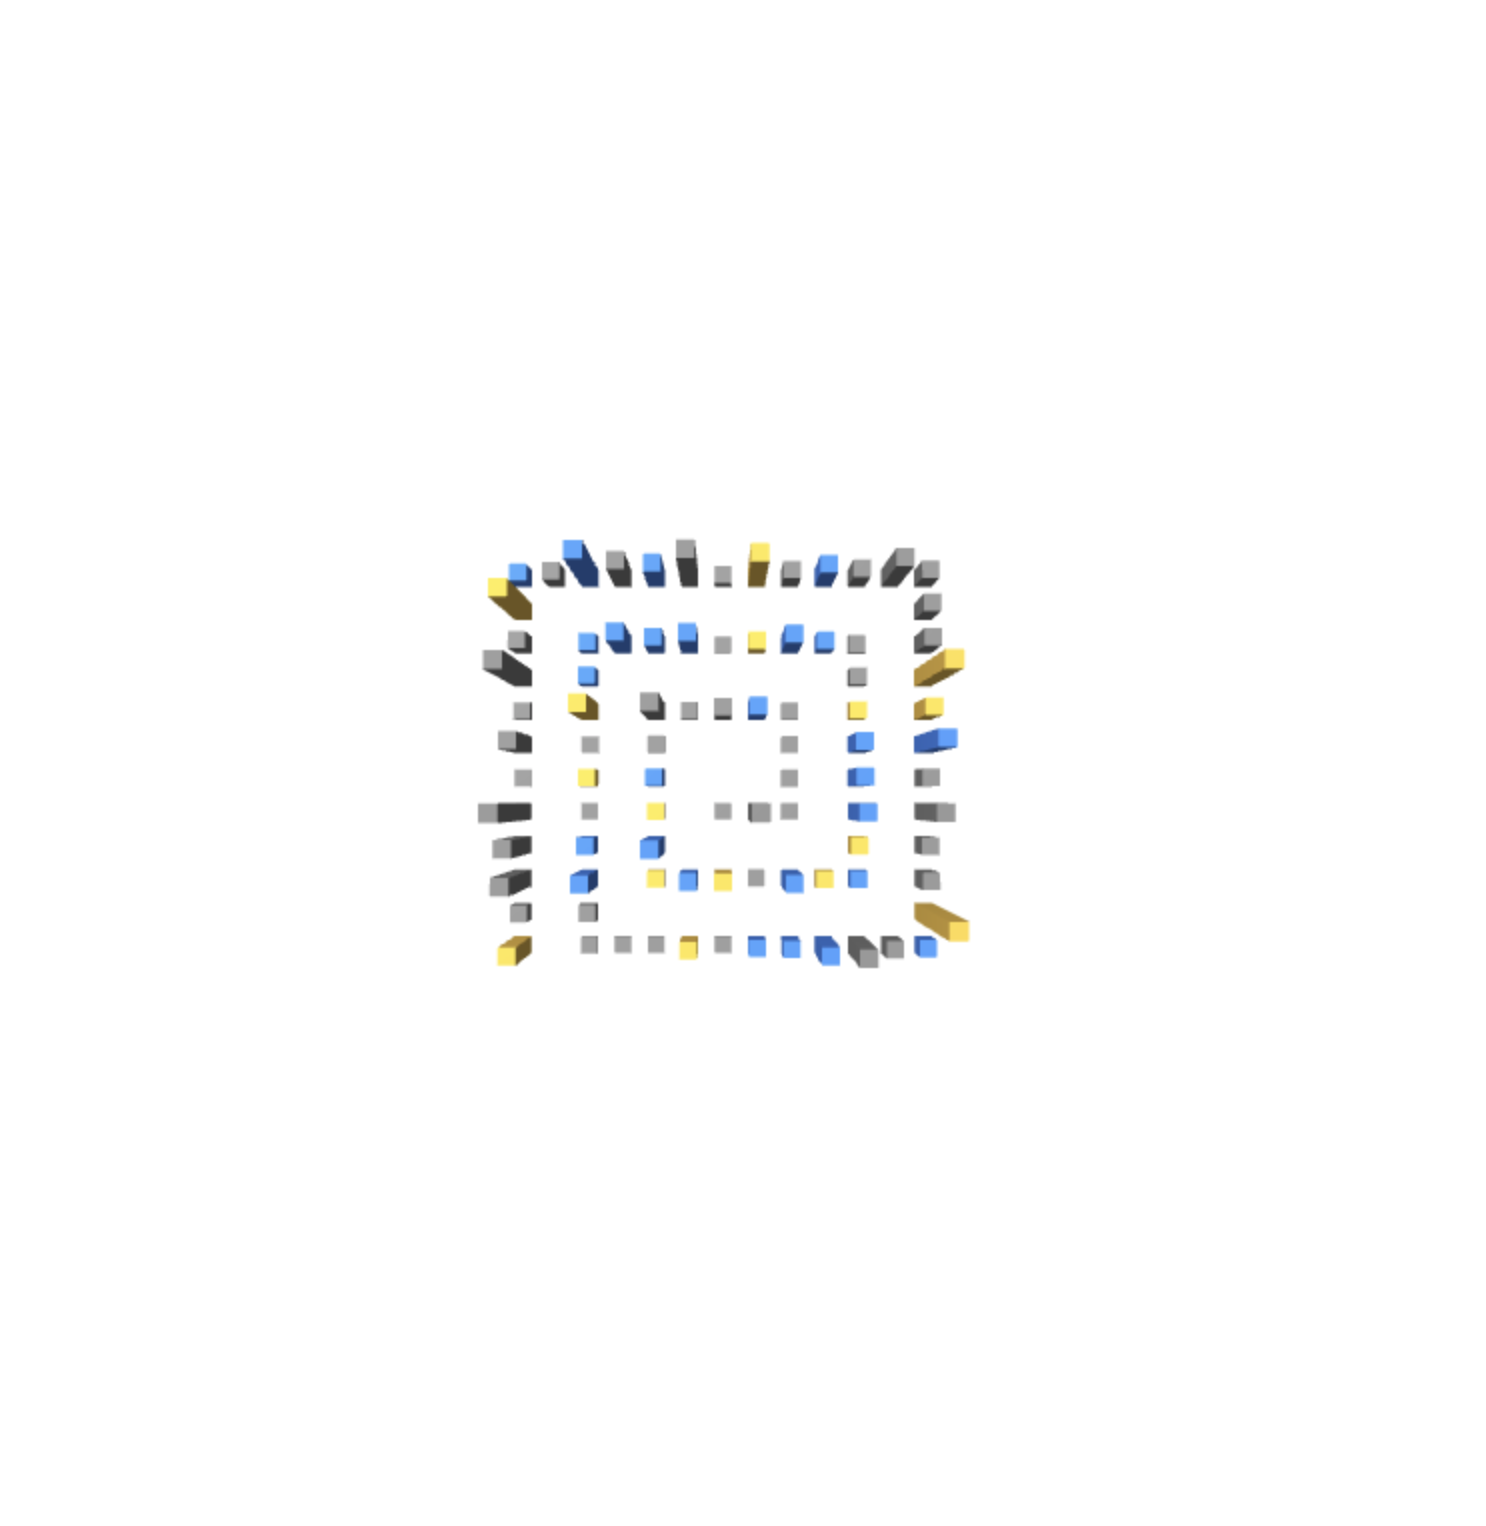
\includegraphics[width=\linewidth]{JetUML_V0S4.png}
        \caption{10 Jan 2015 \linebreak  \#8 Moved to a dedicated ...} 
        \label{fig:JetUML_V0S4}
    \end{subfigure}
    \hspace*{\fill}
    \begin{subfigure}{0.32\textwidth}
        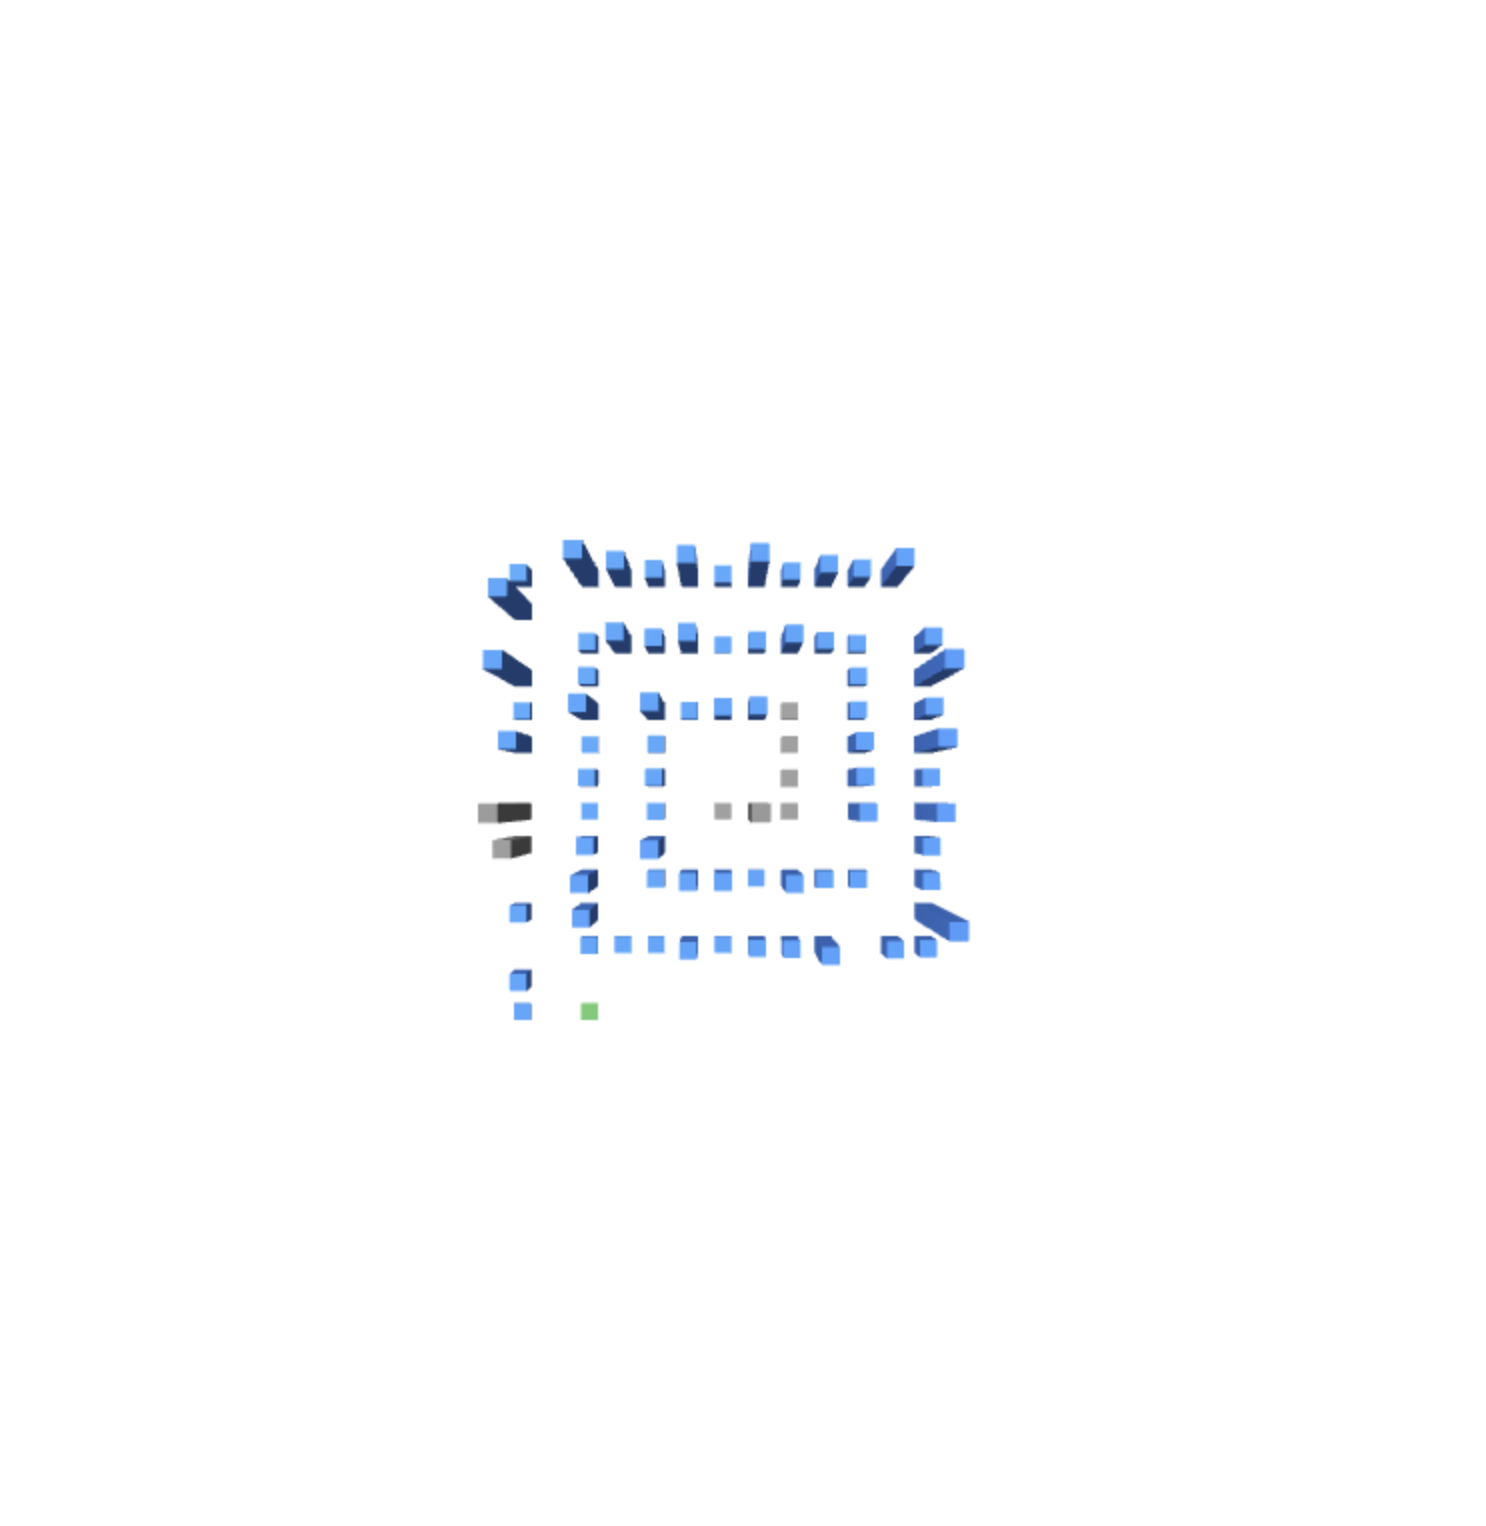
\includegraphics[width=\linewidth]{JetUML_V0S5.png}
        \caption{22 Jan 2015 \linebreak  \#27 Renamed the packages} 
        \label{fig:JetUML_V0S5}
    \end{subfigure}
    \hspace*{\fill}
    \begin{subfigure}{0.32\textwidth}
        
\includegraphics[width=\linewidth]{JetUML_V0S6.png}
        \caption{16 Oct 2015 \linebreak  \#3 New copyright block on ...} 
        \label{fig:JetUML_V0S6}
    \end{subfigure}
    \hspace*{\fill}
    \medskip
    \begin{subfigure}{0.32\textwidth}
        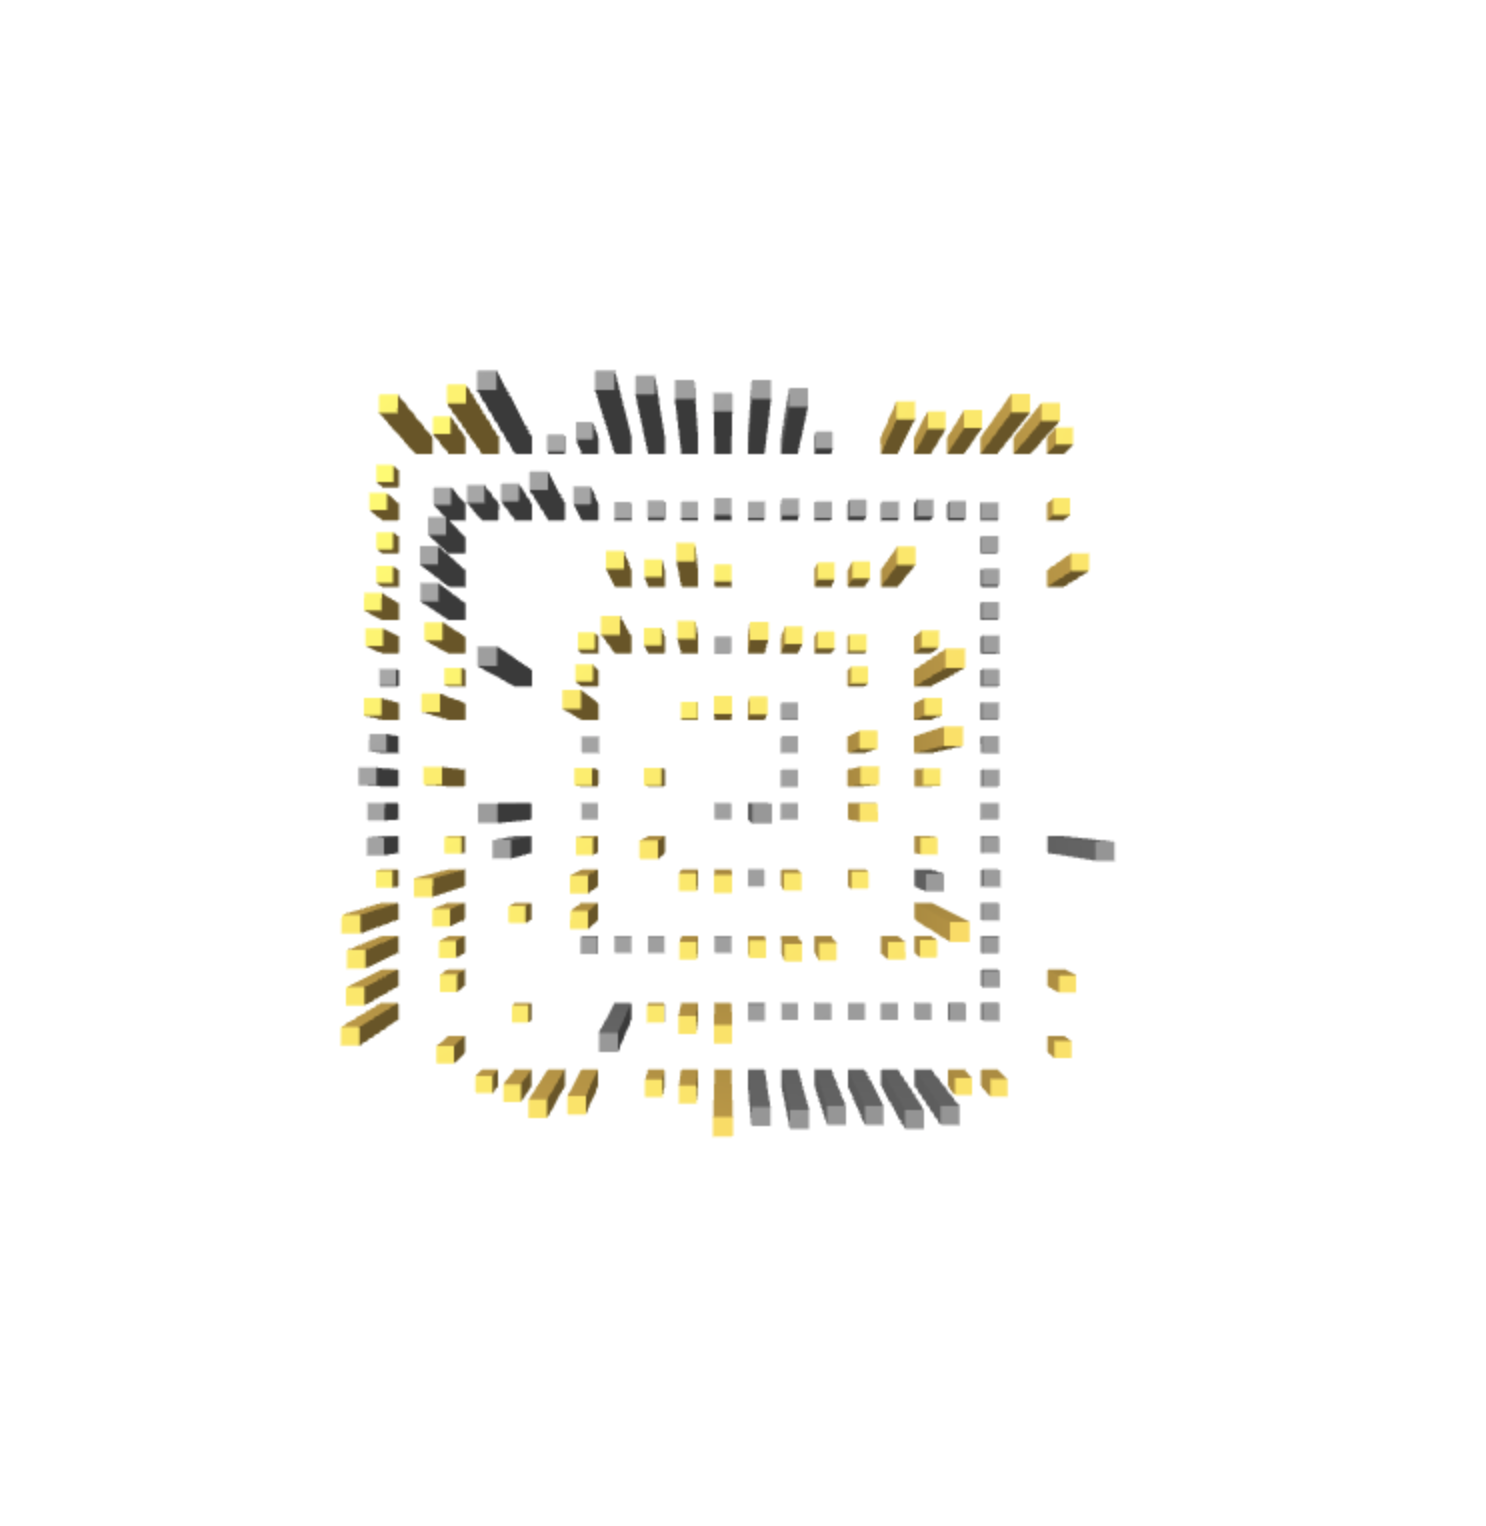
\includegraphics[width=\linewidth]{JetUML_V0S7.png}
        \caption{17 Jan 2016 \linebreak  \#146 Updated the copyright ...}
         \label{fig:JetUML_V0S7}
    \end{subfigure}
    \hspace*{\fill}
    \begin{subfigure}{0.32\textwidth}
        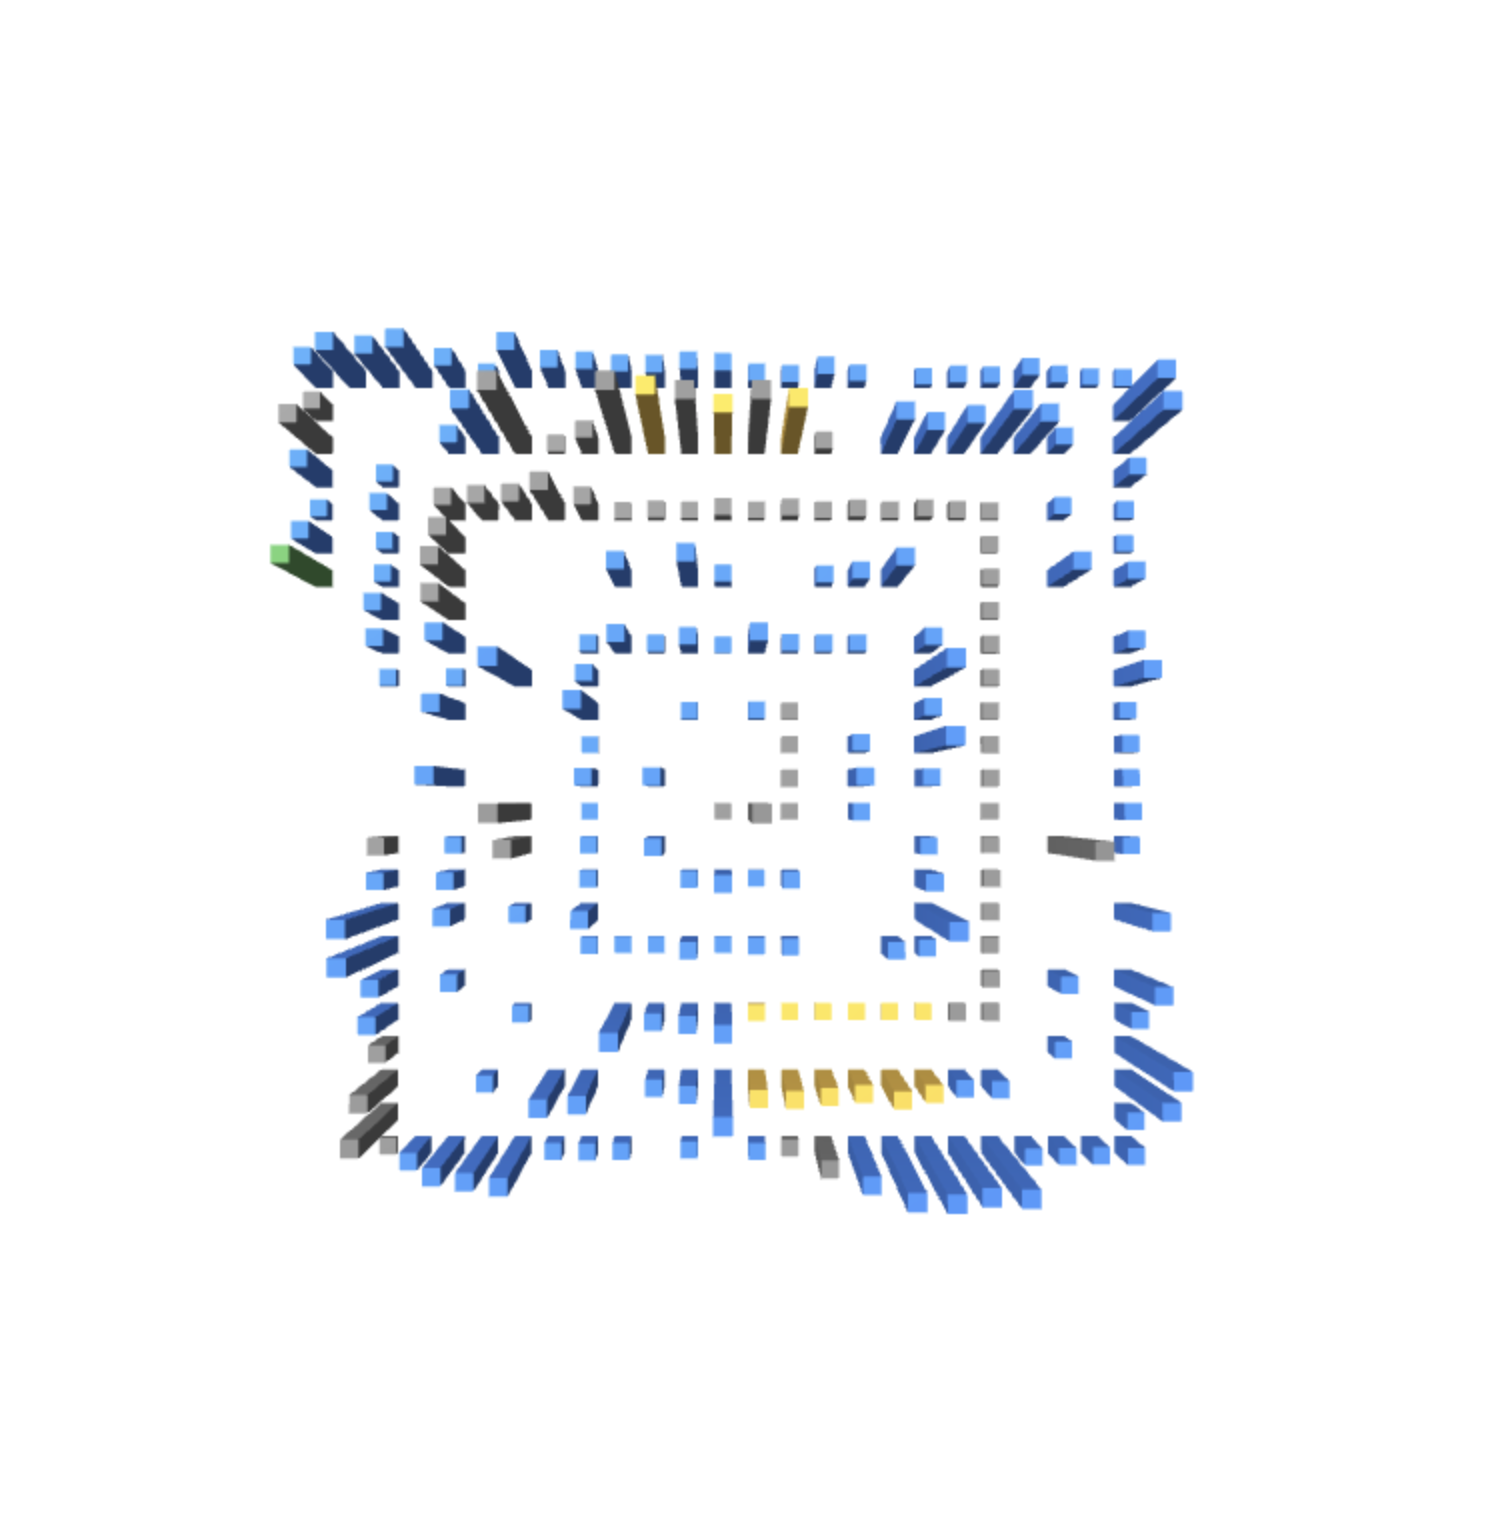
\includegraphics[width=\linewidth]{JetUML_V0S8.png}
        \caption{26 Nov 2017 \linebreak  \#212 Remove stg from name} 
        \label{fig:JetUML_V0S8}
    \end{subfigure}
    \hspace*{\fill}
    \begin{subfigure}{0.32\textwidth}
        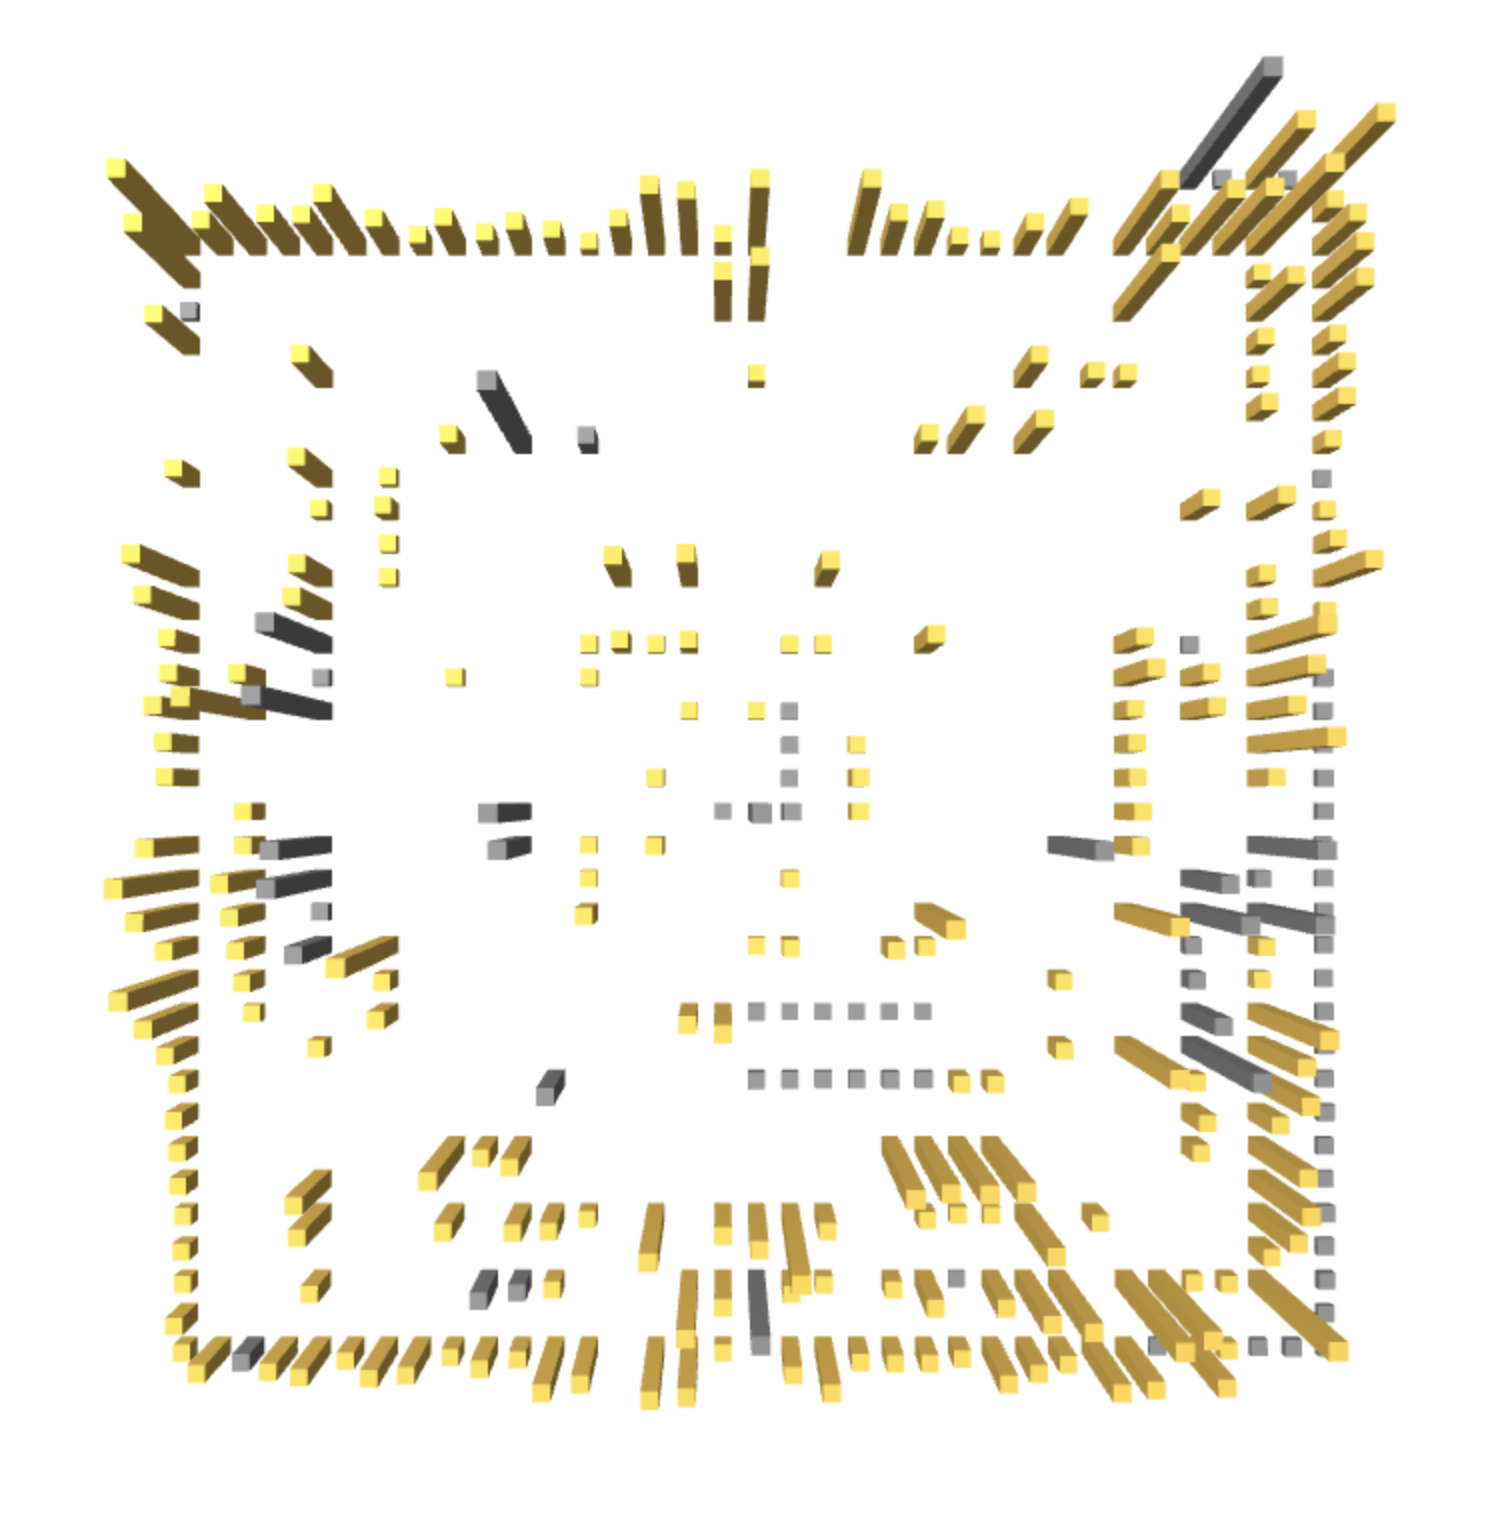
\includegraphics[width=\linewidth]{JetUML_V0S9.png}
        \caption{22 Jul 2020 \linebreak  \#374 Fix copyrights} 
        \label{fig:JetUML_V0S9}
    \end{subfigure}
    \hspace*{\fill}
    \medskip
    \caption{
        Subset of the most significant commits in JetUML. \autoref{fig:JetUML_V0S1_3} presents the first commit. In \autoref{fig:JetUML_V0S2} they pushed the code of Violetta. \autoref{fig:JetUML_V0S3} depicts their first refactoring. In \autoref{fig:JetUML_V0S4} they moved some classes from Violet to Violetta. In \autoref{fig:JetUML_V0S5} they moved most of them under JetUML. In \autoref{fig:JetUML_V0S6}, \autoref{fig:JetUML_V0S7} and \autoref{fig:JetUML_V0S9} present three refactoring activities to fix copyrights. In \autoref{fig:JetUML_V0S8} most entities are painted blue because they changed their path.} 
    \label{fig:JetUML_V0}
\end{figure}

\clearpage
\section{JetUML – The Beginnings}
\textbf{Visualization goal:}
With this visualization, we present how the repository evolved through its first six months. 
The authors of JetUML made seven pre-releases of the system during this interval of time.
We want to demonstrate the effectiveness of aging by showing what a strategy of one month with ten steps looks like. 


View specification adopted: 
\begin{itemize}
    \item \texttt{versionGroupingStrategy}: timestamp.
    \item \texttt{versionGroupingChunkSize}: 2,629,743 (1 month). 
    \item \texttt{colorPalette}: default.
    \item \texttt{agingGroupingStrategy}: timestamp.
    \item \texttt{agingStepSize}: 2,629,743 (1 month).
    \item \texttt{agingSteps}: 10 steps.
    \item \texttt{mapperMetricName}: SIZE. 
    \item \texttt{fileTypeShape}: all BOX. 
    \item \texttt{fileTypeOpacity}: all 1. 
\end{itemize}

\textbf{Results:}
\autoref{fig:JetUML_V1} shows the evolution of JetUML in each month of its first half-year development. \autoref{fig:JetUML_V1S1} shows the state of the repository after the first month. All entities are painted with the color representing the last action of the file. All the colors are bright because the age of all files is set to 0 since the time elapsed between their previous action and the last commit of the visualization is a maximum of one month. Furthermore, most of the moved files have the extension \texttt{.properties}, and they were involved in a refactoring activity since their path changed from \quotes{src/ca/mcgill/cs/stg/jetuml/...} to \quotes{src/ca/mcgill/cs/stg/jetuml/diagrams/...}.  At the end of their first month of activity, they made 127 commits and they worked with 135 files. The second month is depicted in \autoref{fig:JetUML_V1S2}. Here we can easily spot older entities as they are darker than others. This means that some files had not been touched since the first month at the end of the second month. In the third and the fourth month, more or less the same amount of files were updated. However, in the fifth month, only three entities were modified; consequently, all the others are darker because they are older. 
At the end of the sixth month, two entities were added and modified. However, most of the entities were still getting older. 

\bigbreak
\textbf{Conclusion:}
We have seen how different is the timestamp strategy compared to what we saw \autoref{fig:JetUML_V0}. Here, the number of frames does not depend on the number of commits but on the number of months of history. 
The choice of the aging strategy played a crucial role in this visualization. It highlighted the updated entities without hiding the last action made on the others. Looking at \autoref{fig:JetUML_V1S6}, we can see that many files were added and never touched because their color looks dark green. This inactivity on the files may be related to the file type. Java files might be more prone to be updated rather than configuration files such as YAML files. Nonetheless, the choice of representing all the entities with the same shape (BOX) limits our visualization because we cannot infer their type in any way. 

% With this visualization, we want to see how all JetUML files evolved through time. 
% JetUML does not seem to have a fixed release cycle.
% Since its history spans eight years of activity; we initially chose a timestamp grouping strategy of one month. 
% As a consequence, we have 89 AnimationFrames. 
% In this first visualization, we do not care about the FileType of entities; we are interested in all of them. 
% Grouping commits monthly; we applied the same strategy to the aging to see how many months had passed since an entity was modified. 
% To summarize, the view specification of this visualization is the following:

% Figure \ref{fig:JetUML_V1} shows the first 6 month of evolution of JetUML. 
% We can infer many things by looking at these figures. In figure \ref{fig:JetUML_V1S1} 7 entities have been moved. 
% Most of them are files with the extension \texttt{.properties}, and perhaps they were involved in a refactoring activity since their path changed from
% \texttt{src/ca/mcgill/cs/stg/jetuml/...} to \texttt{src/ca/mcgill/cs/stg/jetuml/diagrams/...}. 
% At the end of their first month of activity, they had 135 files and made 127 commits. 
% We can see many files are still green. This means that they were added but never touched after. 
% An issue with this visualization is that we cannot distinguish Java files from others. 
% These added files are images. Therefore it is not a surprise that once added; they are never modified in the future. 
% In figure \ref{fig:JetUML_V1S2} where the second month is represented, we can see that some entities have a darker color. 
% This means that during the second month, they were not touched. 
% Comparing all the figures until figure \ref{fig:JetUML_V1S6} we can notice that many entities have the same behavior. 
% They were added and updated in the first month of activity (this is why they are yellow), and then they were never touched, becoming darker and darker each month. 

\begin{figure}[ht]
    \begin{subfigure}{0.48\textwidth}
    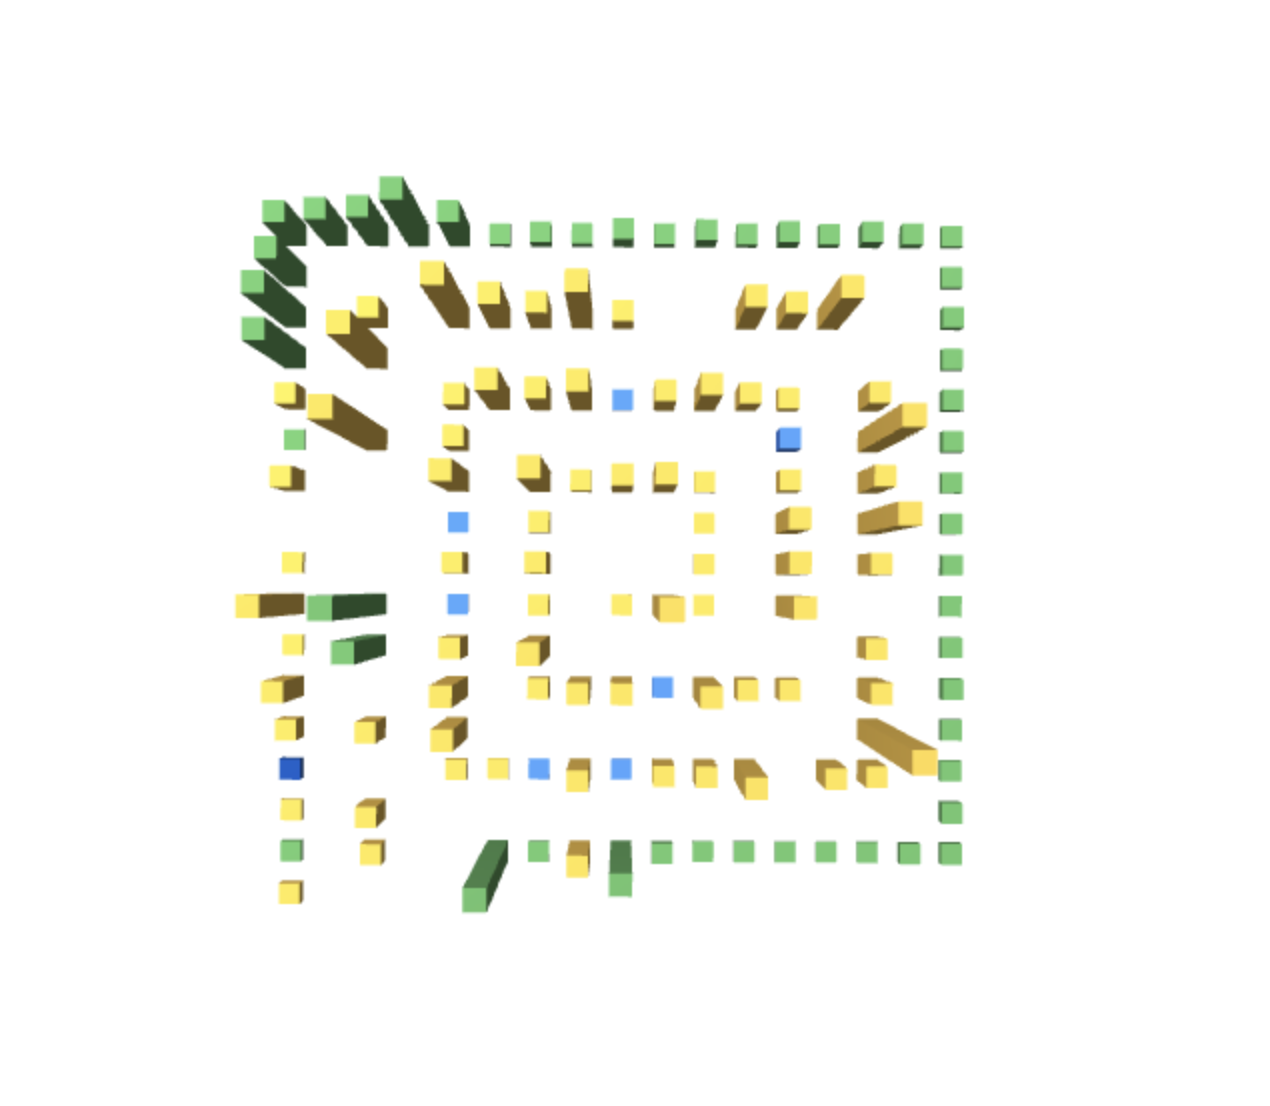
\includegraphics[width=\linewidth]{JetUML_V1S1.png}
    \caption{Month 1 - Feb 07, 2015 } \label{fig:JetUML_V1S1}
    \end{subfigure}\hspace*{\fill}
    \begin{subfigure}{0.48\textwidth}
        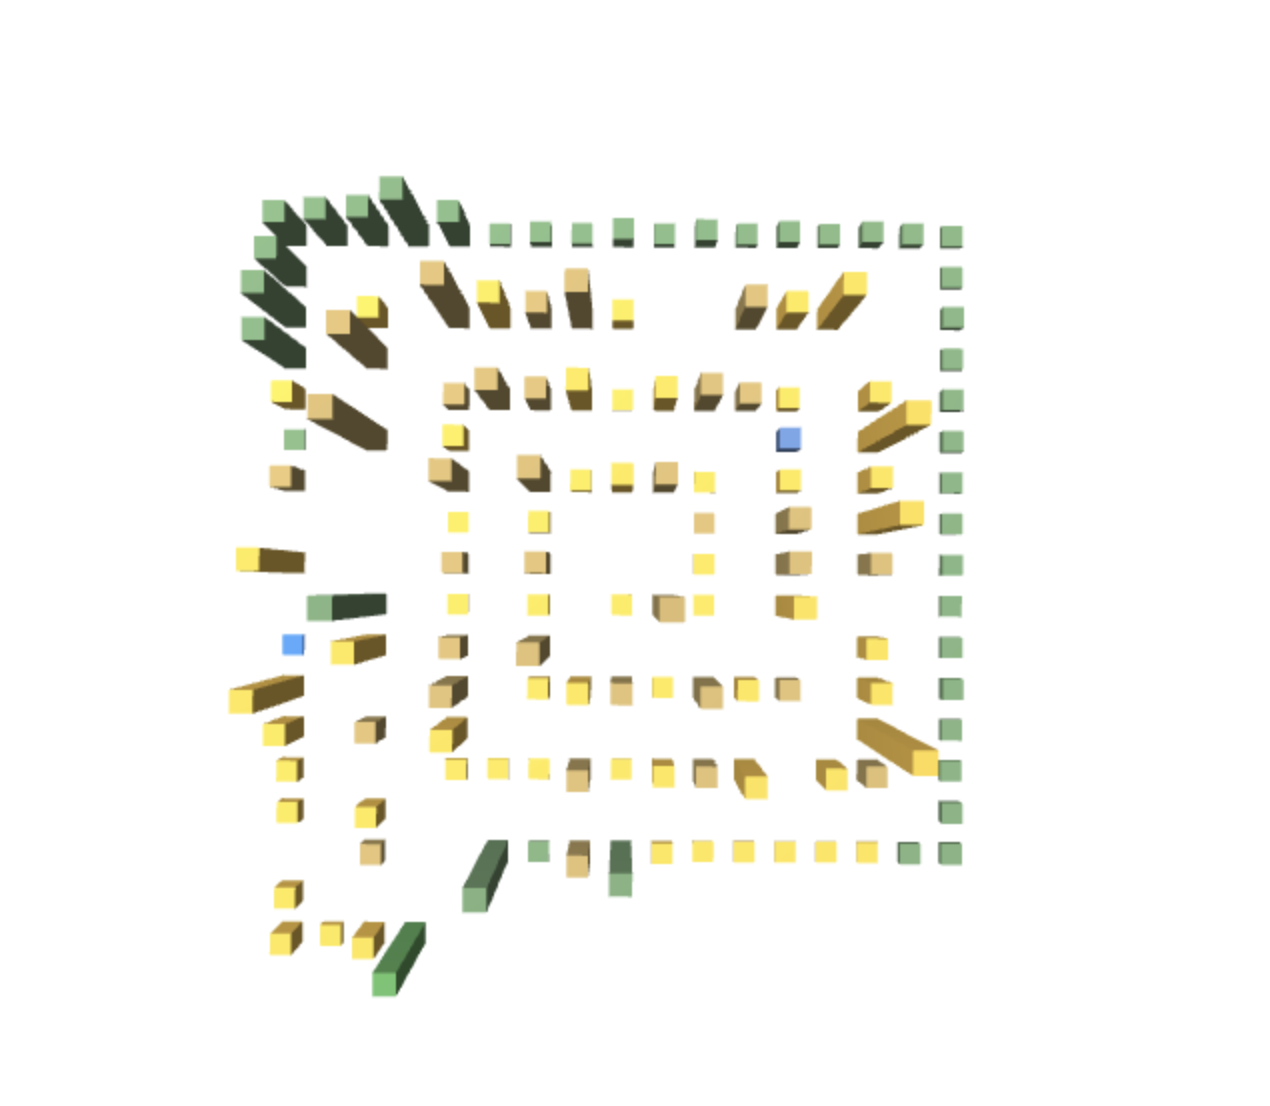
\includegraphics[width=\linewidth]{JetUML_V1S2.png}
        \caption{Month 2 - Mar 07, 2015} \label{fig:JetUML_V1S2}
    \end{subfigure}
    
    \medskip
    \begin{subfigure}{0.48\textwidth}
        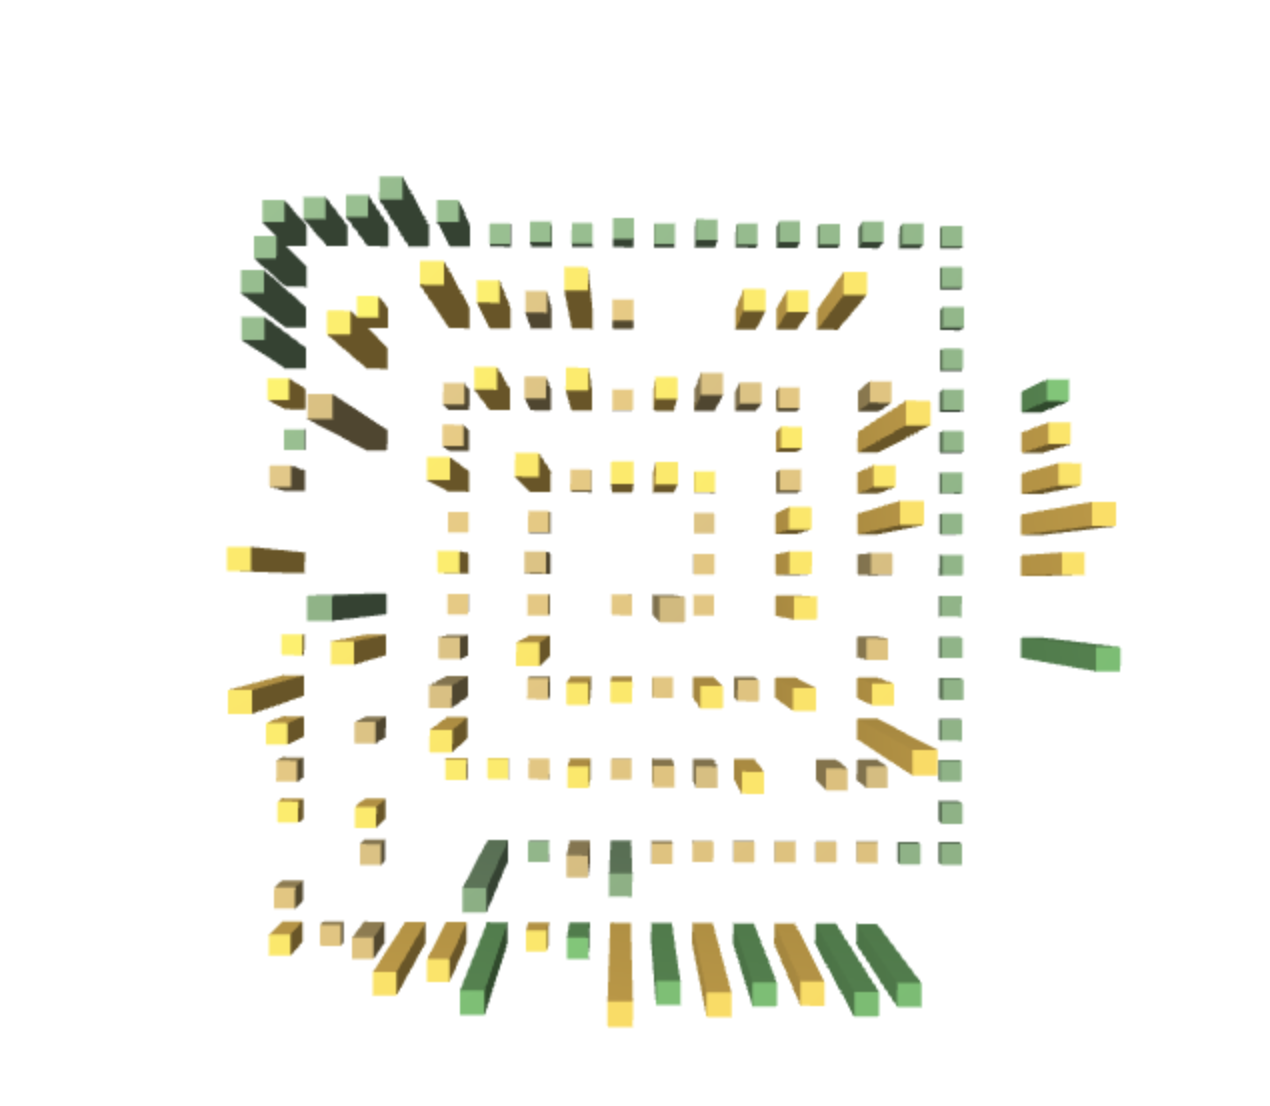
\includegraphics[width=\linewidth]{JetUML_V1S3.png}
        \caption{Month 3 - Apr 07, 2015} \label{fig:JetUML_V1S3}
    \end{subfigure}\hspace*{\fill}
    \begin{subfigure}{0.48\textwidth}
    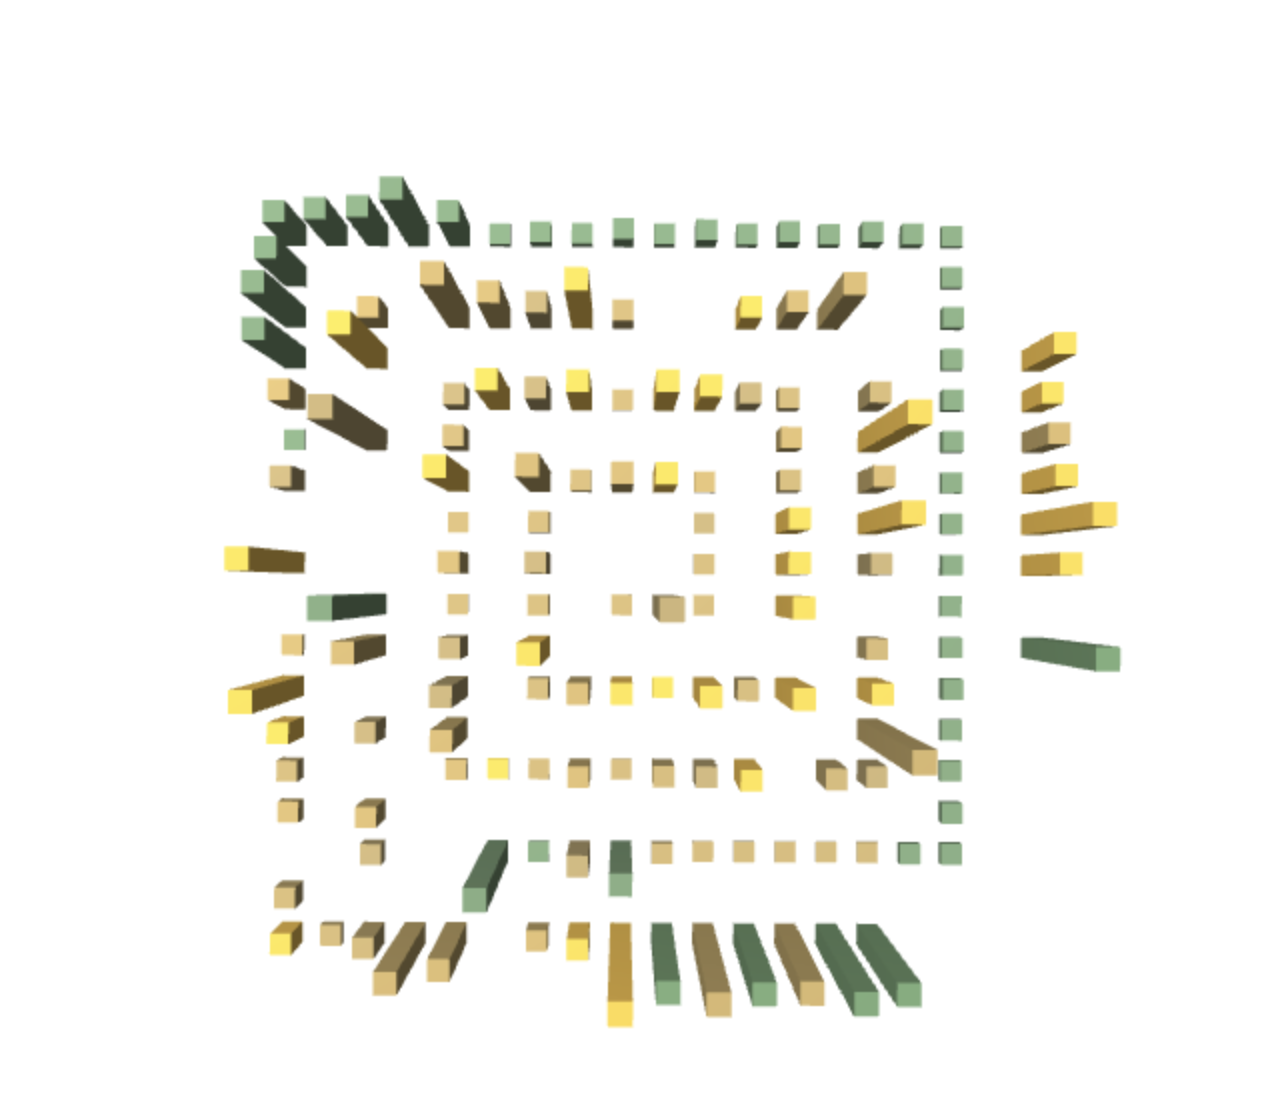
\includegraphics[width=\linewidth]{JetUML_V1S4.png}
    \caption{Month 4 - May 07, 2015} \label{fig:JetUML_V1S4}
    \end{subfigure}
    
    \medskip
    \begin{subfigure}{0.48\textwidth}
        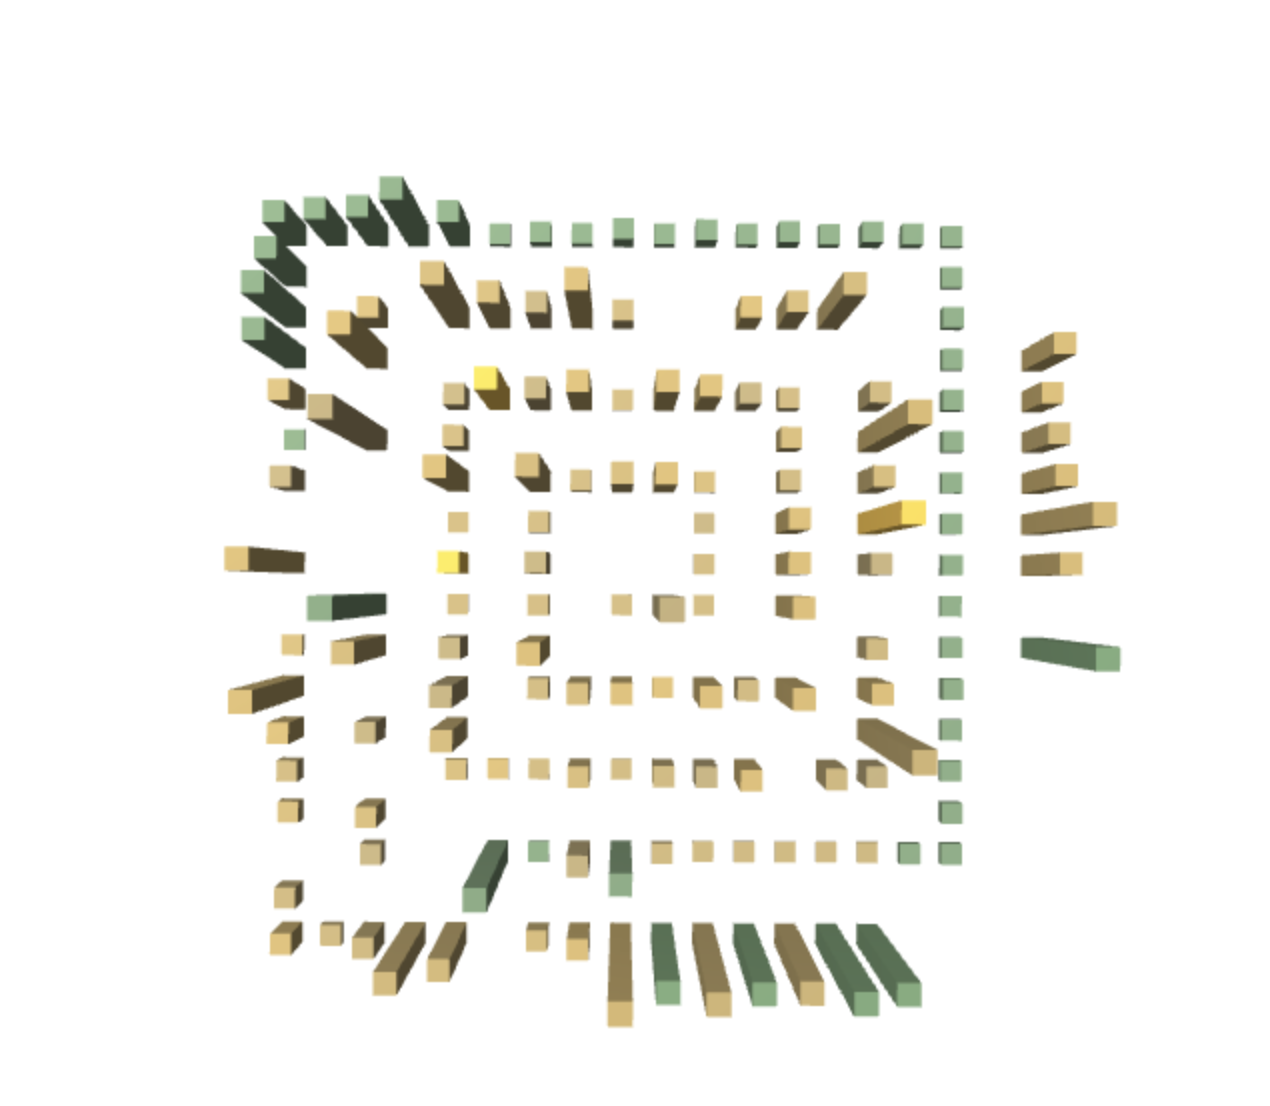
\includegraphics[width=\linewidth]{JetUML_V1S5.png}
        \caption{Month 5 - Jun 07, 2015} \label{fig:JetUML_V1S5}
    \end{subfigure}\hspace*{\fill}
    \begin{subfigure}{0.48\textwidth}
        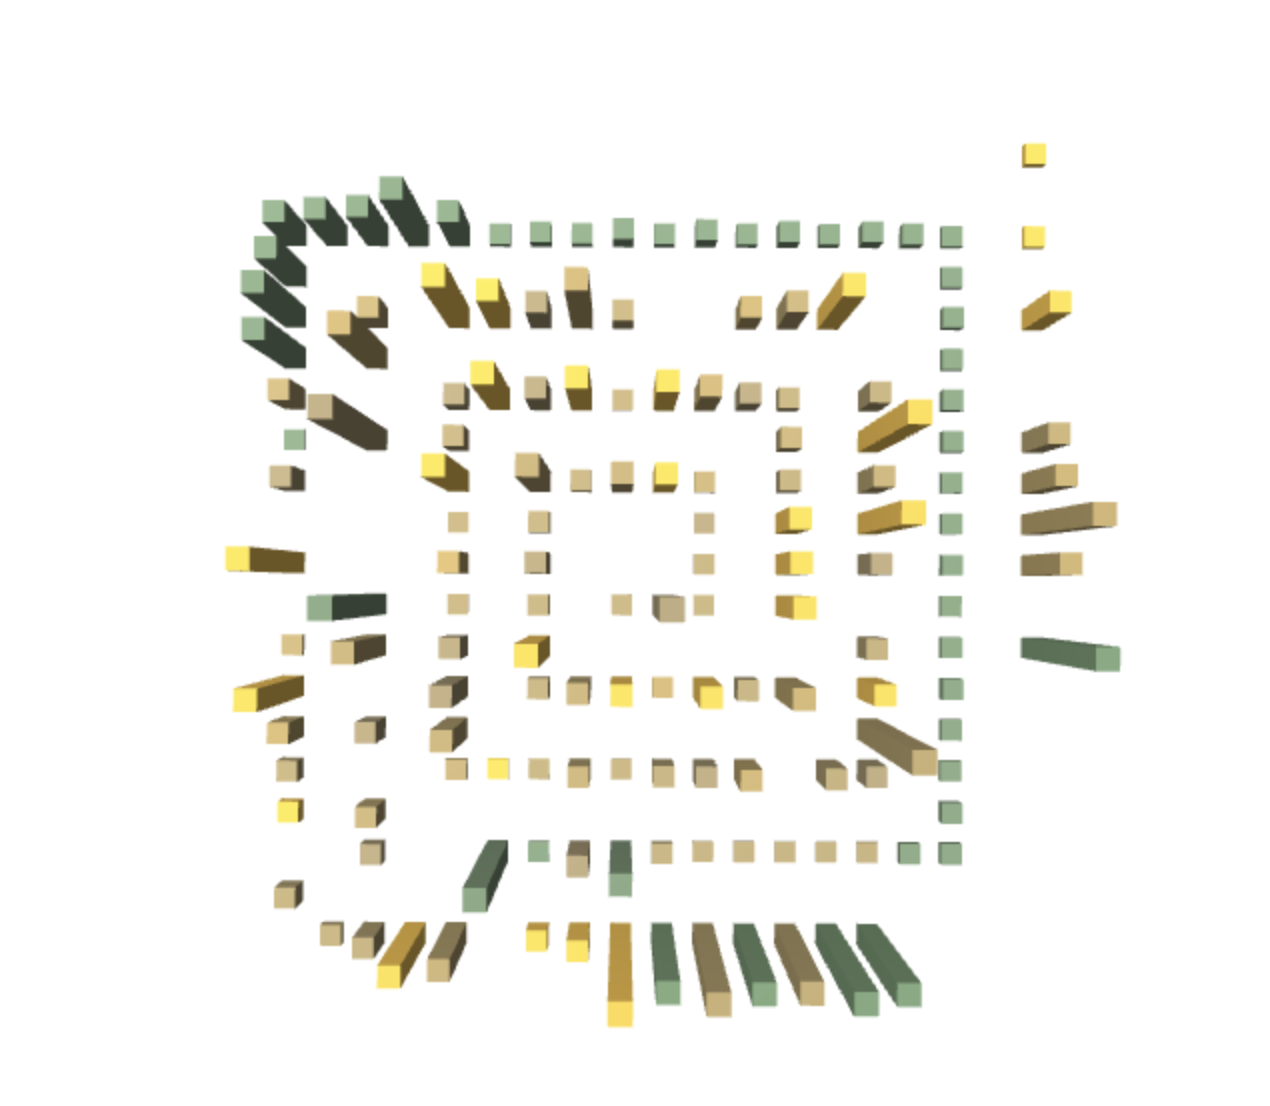
\includegraphics[width=\linewidth]{JetUML_V1S6.png}
        \caption{Month 6 - Jul 07, 2015} \label{fig:JetUML_V1S6}
    \end{subfigure}
    
    \caption{First six months of JetUML's evolution.} 
    \label{fig:JetUML_V1}
\end{figure}
\clearpage
\section{JetUML – Year by Year}
\textbf{Visualization goal:}
In this third and last visualization of JetUML, we study the entire evolution of the system, with a focus on Java files. 
We use the shape and opacity property of a ViewFigure to distinguish Java files from others.
We adopt a timestamp grouping strategy with one year to display the evolution. We also use a timestamp strategy for the aging, with ten steps and one month time window. This means that grey entities represent files that have not been updated in the last 10 months from the time of the displayed AnimationFrame. 
\begin{itemize}
    \item \texttt{versionGroupingStrategy}: timestamp.
    \item \texttt{versionGroupingChunkSize}: 31,556,926 (1 year). 
    \item \texttt{colorPalette}: default.
    \item \texttt{agingGroupingStrategy}: timestamp.
    \item \texttt{agingStepSize}: 2,629,743 (1 month).
    \item \texttt{agingSteps}: 10 steps. 
    \item \texttt{mapperMetricName}: SLOC. 
    \item \texttt{fileTypeShape}: Java -> BOX, OTHERS -> SPHERE. 
    \item \texttt{fileTypeOpacity}: Java -> max, OTHERS -> low. 
\end{itemize}

\textbf{Results:}
The whole evolution of JetUML is depicted in \autoref{fig:JetUML_V3}. As we notice, it is straightforward to distinguish Java files from others because they have different shapes (cuboids vs. hemispheres)  and other files are less opaque. After the first year of development, the state of the repository is shown in \autoref{fig:JetUML_V3S1}. We notice that the Java files have more or less the same age. This means that all of them were updated after the second month otherwise, they would be grey. The system grew at the end of the second year, as shown in \autoref{fig:JetUML_V3S2}, and now we can see some grey entities. Most of them are in the middle, meaning that the "core" files, or the oldest files, were not touched after the fourteenth month.  \autoref{fig:JetUML_V3S3} shows the state of the repository at the end of the third year. The system grew, and all the Java files were updated recently. Considering what we have seen in the first visualization, they had to change the path from all the Java files (\autoref{fig:JetUML_V0S8}). Perhaps this can be why all the entities were updated, and some ViewFigures are painted blue. 
The fourth year of development, shown in  \autoref{fig:JetUML_V3S4}, recorded a growth in the first month; therefore, almost all the entities have a different color.
However, they are dark, meaning they are old. 
\autoref{fig:JetUML_V3S5},  \autoref{fig:JetUML_V3S6} and  \autoref{fig:JetUML_V3S7} shows how the system evolved through the fifth, sixth, and seventh years. The fifth-year recorded an intense activity compared to what we saw in the fourth year. Lots of files were added, and most of the classes of the system were modified. Furthermore, the system's center is slowly disappearing, meaning old Java files have been replaced. In the sixth and seventh years, non-Java files were added, and some Java classes were updated outside the system's core. Finally, the last year, represented by \autoref{fig:JetUML_V3S8}, did not record such a huge activity on the system. It became inactive as almost all the entities are grey, meaning that they were not touched in the last ten months of evolution. However, in this frame, the two tallest entities of the system appeared. Two Java files were added (they were not present the year before) and rapidly became the biggest files in the repository.  
\bigbreak
\textbf{Conclusion:}
With this visualization, we have seen JetUML from another point of view. The year visualization works very well with systems like JetUML with a large history. In fact, with just eight AnimationFrames, we depicted the evolution of the last 9 years. In addition, we identified moments in the past when the development process was more intense. 
\bigbreak

\begin{figure}[ht]
    \begin{subfigure}{0.50\textwidth}
        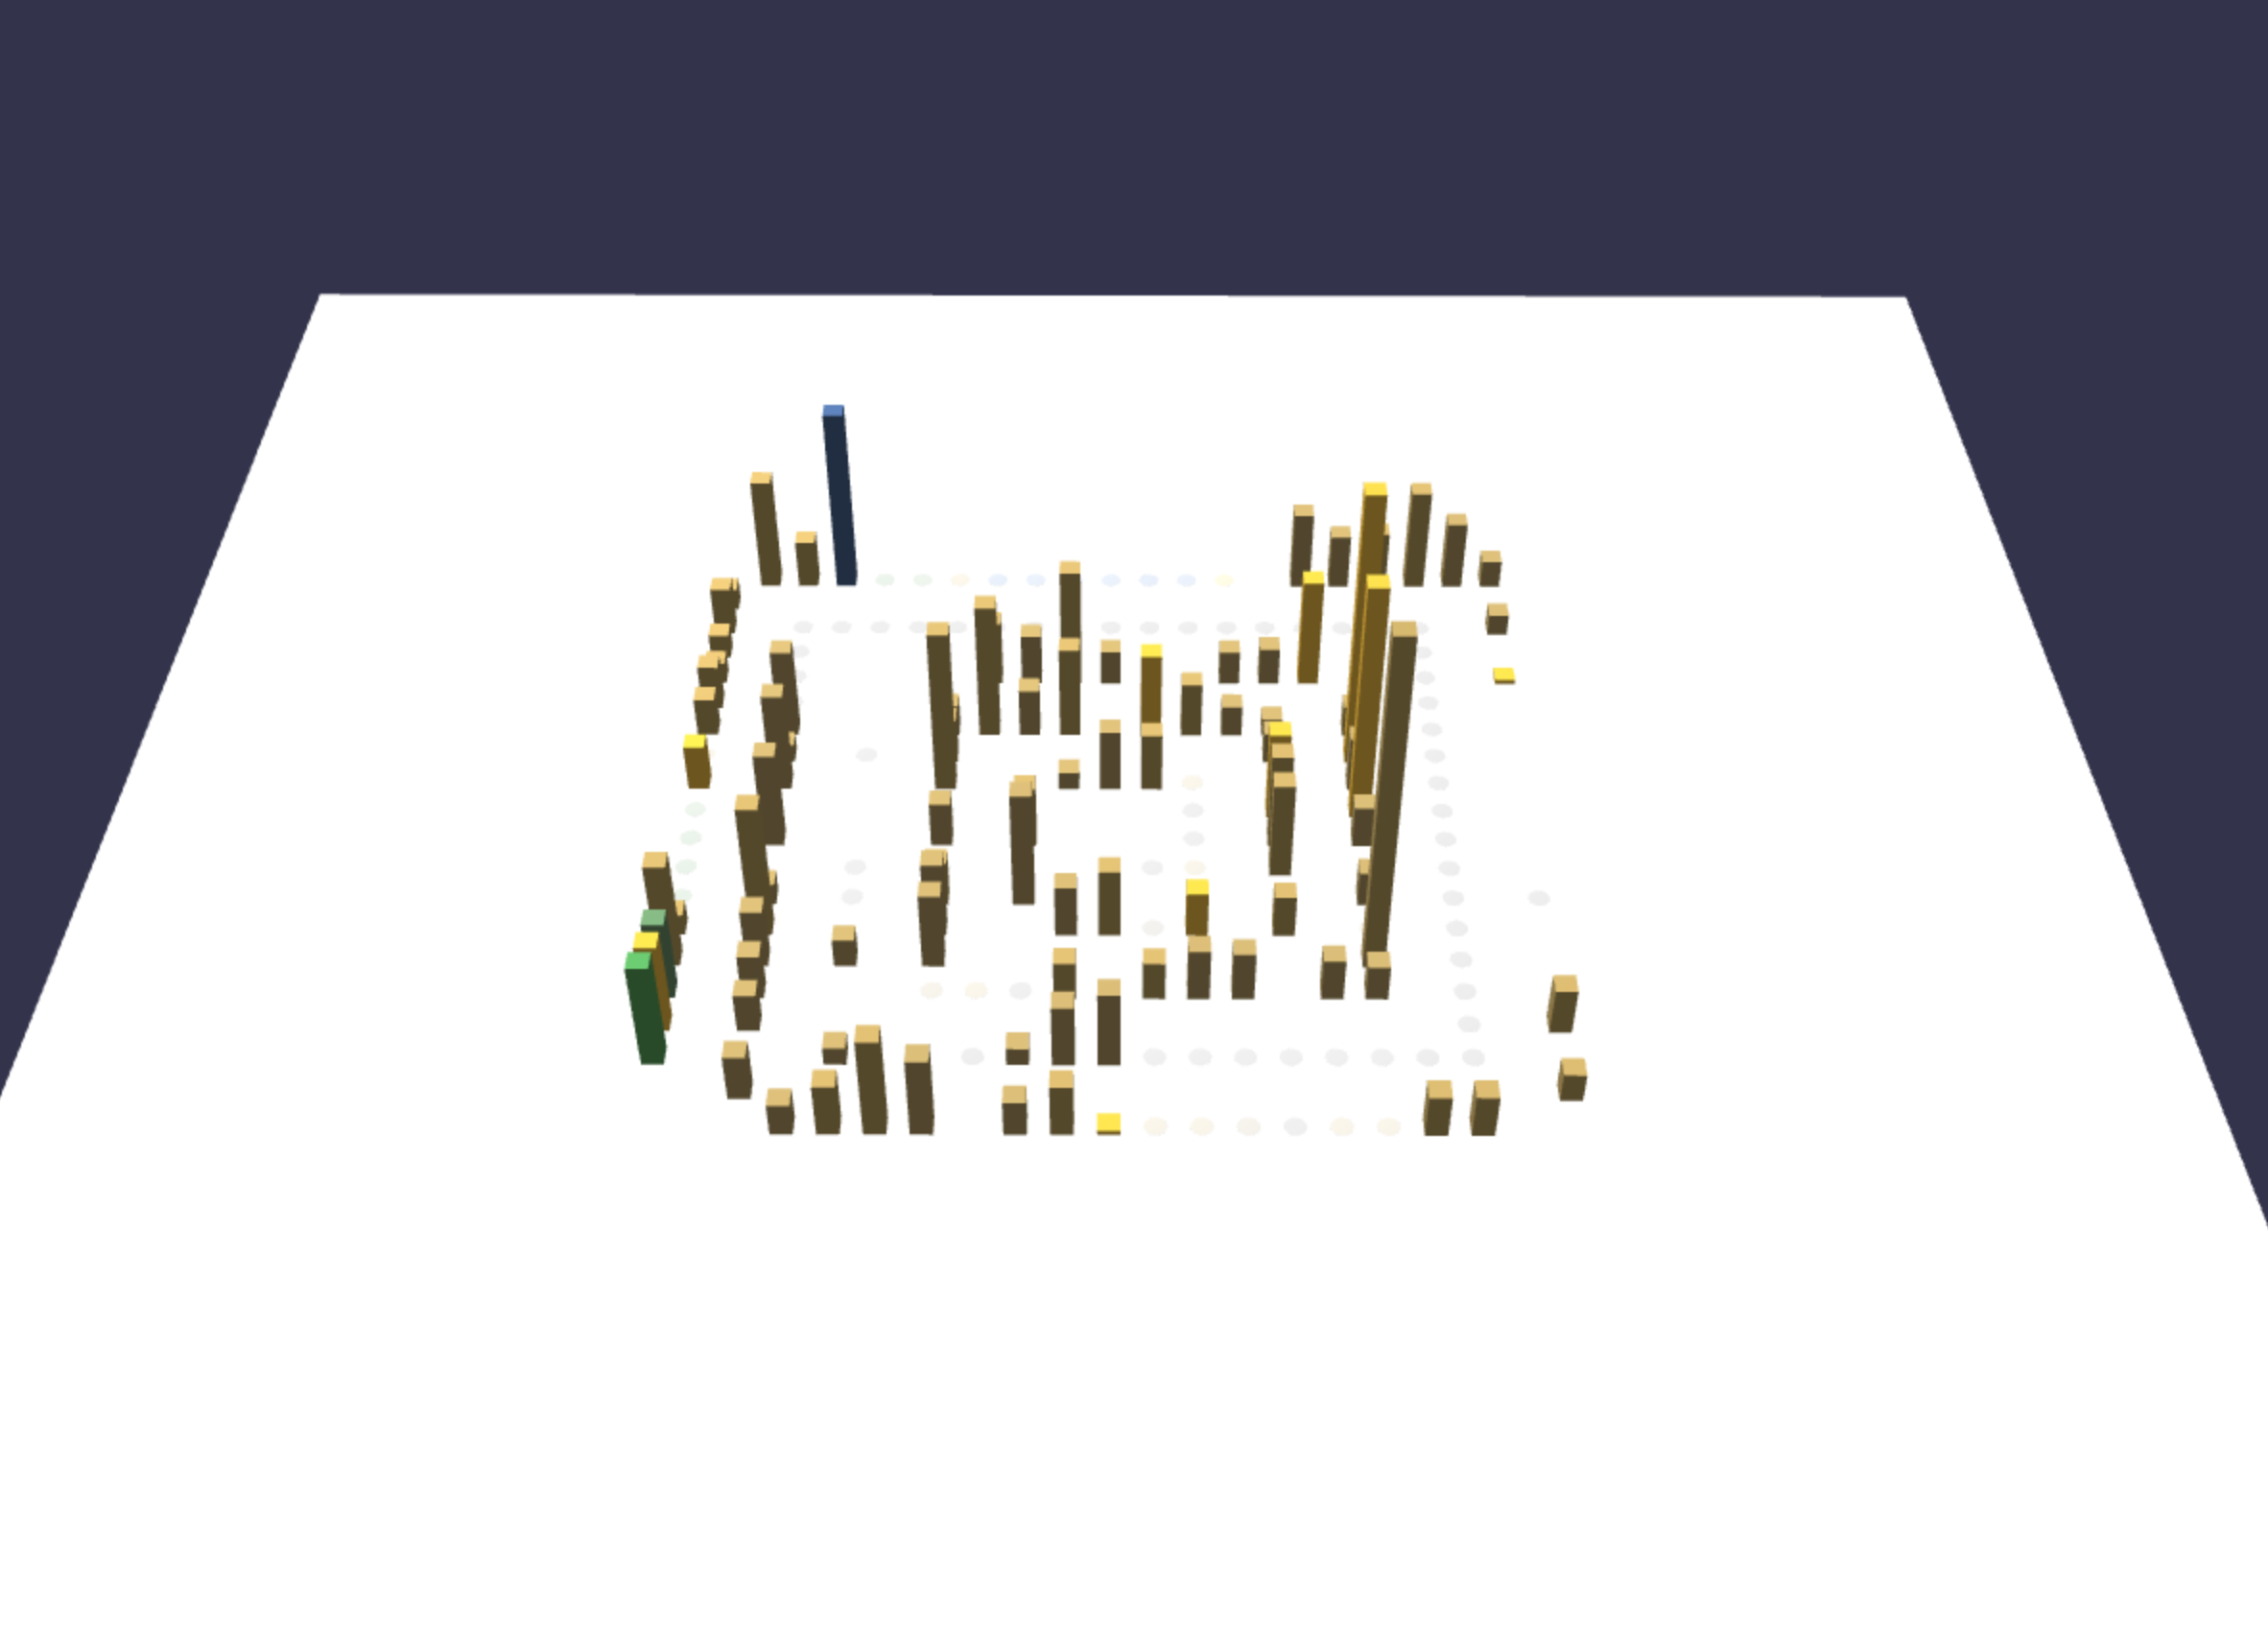
\includegraphics[width=\linewidth]{JetUML_V3S1.png}
        \caption{Year 1} 
        \label{fig:JetUML_V3S1}
    \end{subfigure}\hspace*{\fill}
    \begin{subfigure}{0.50\textwidth}
        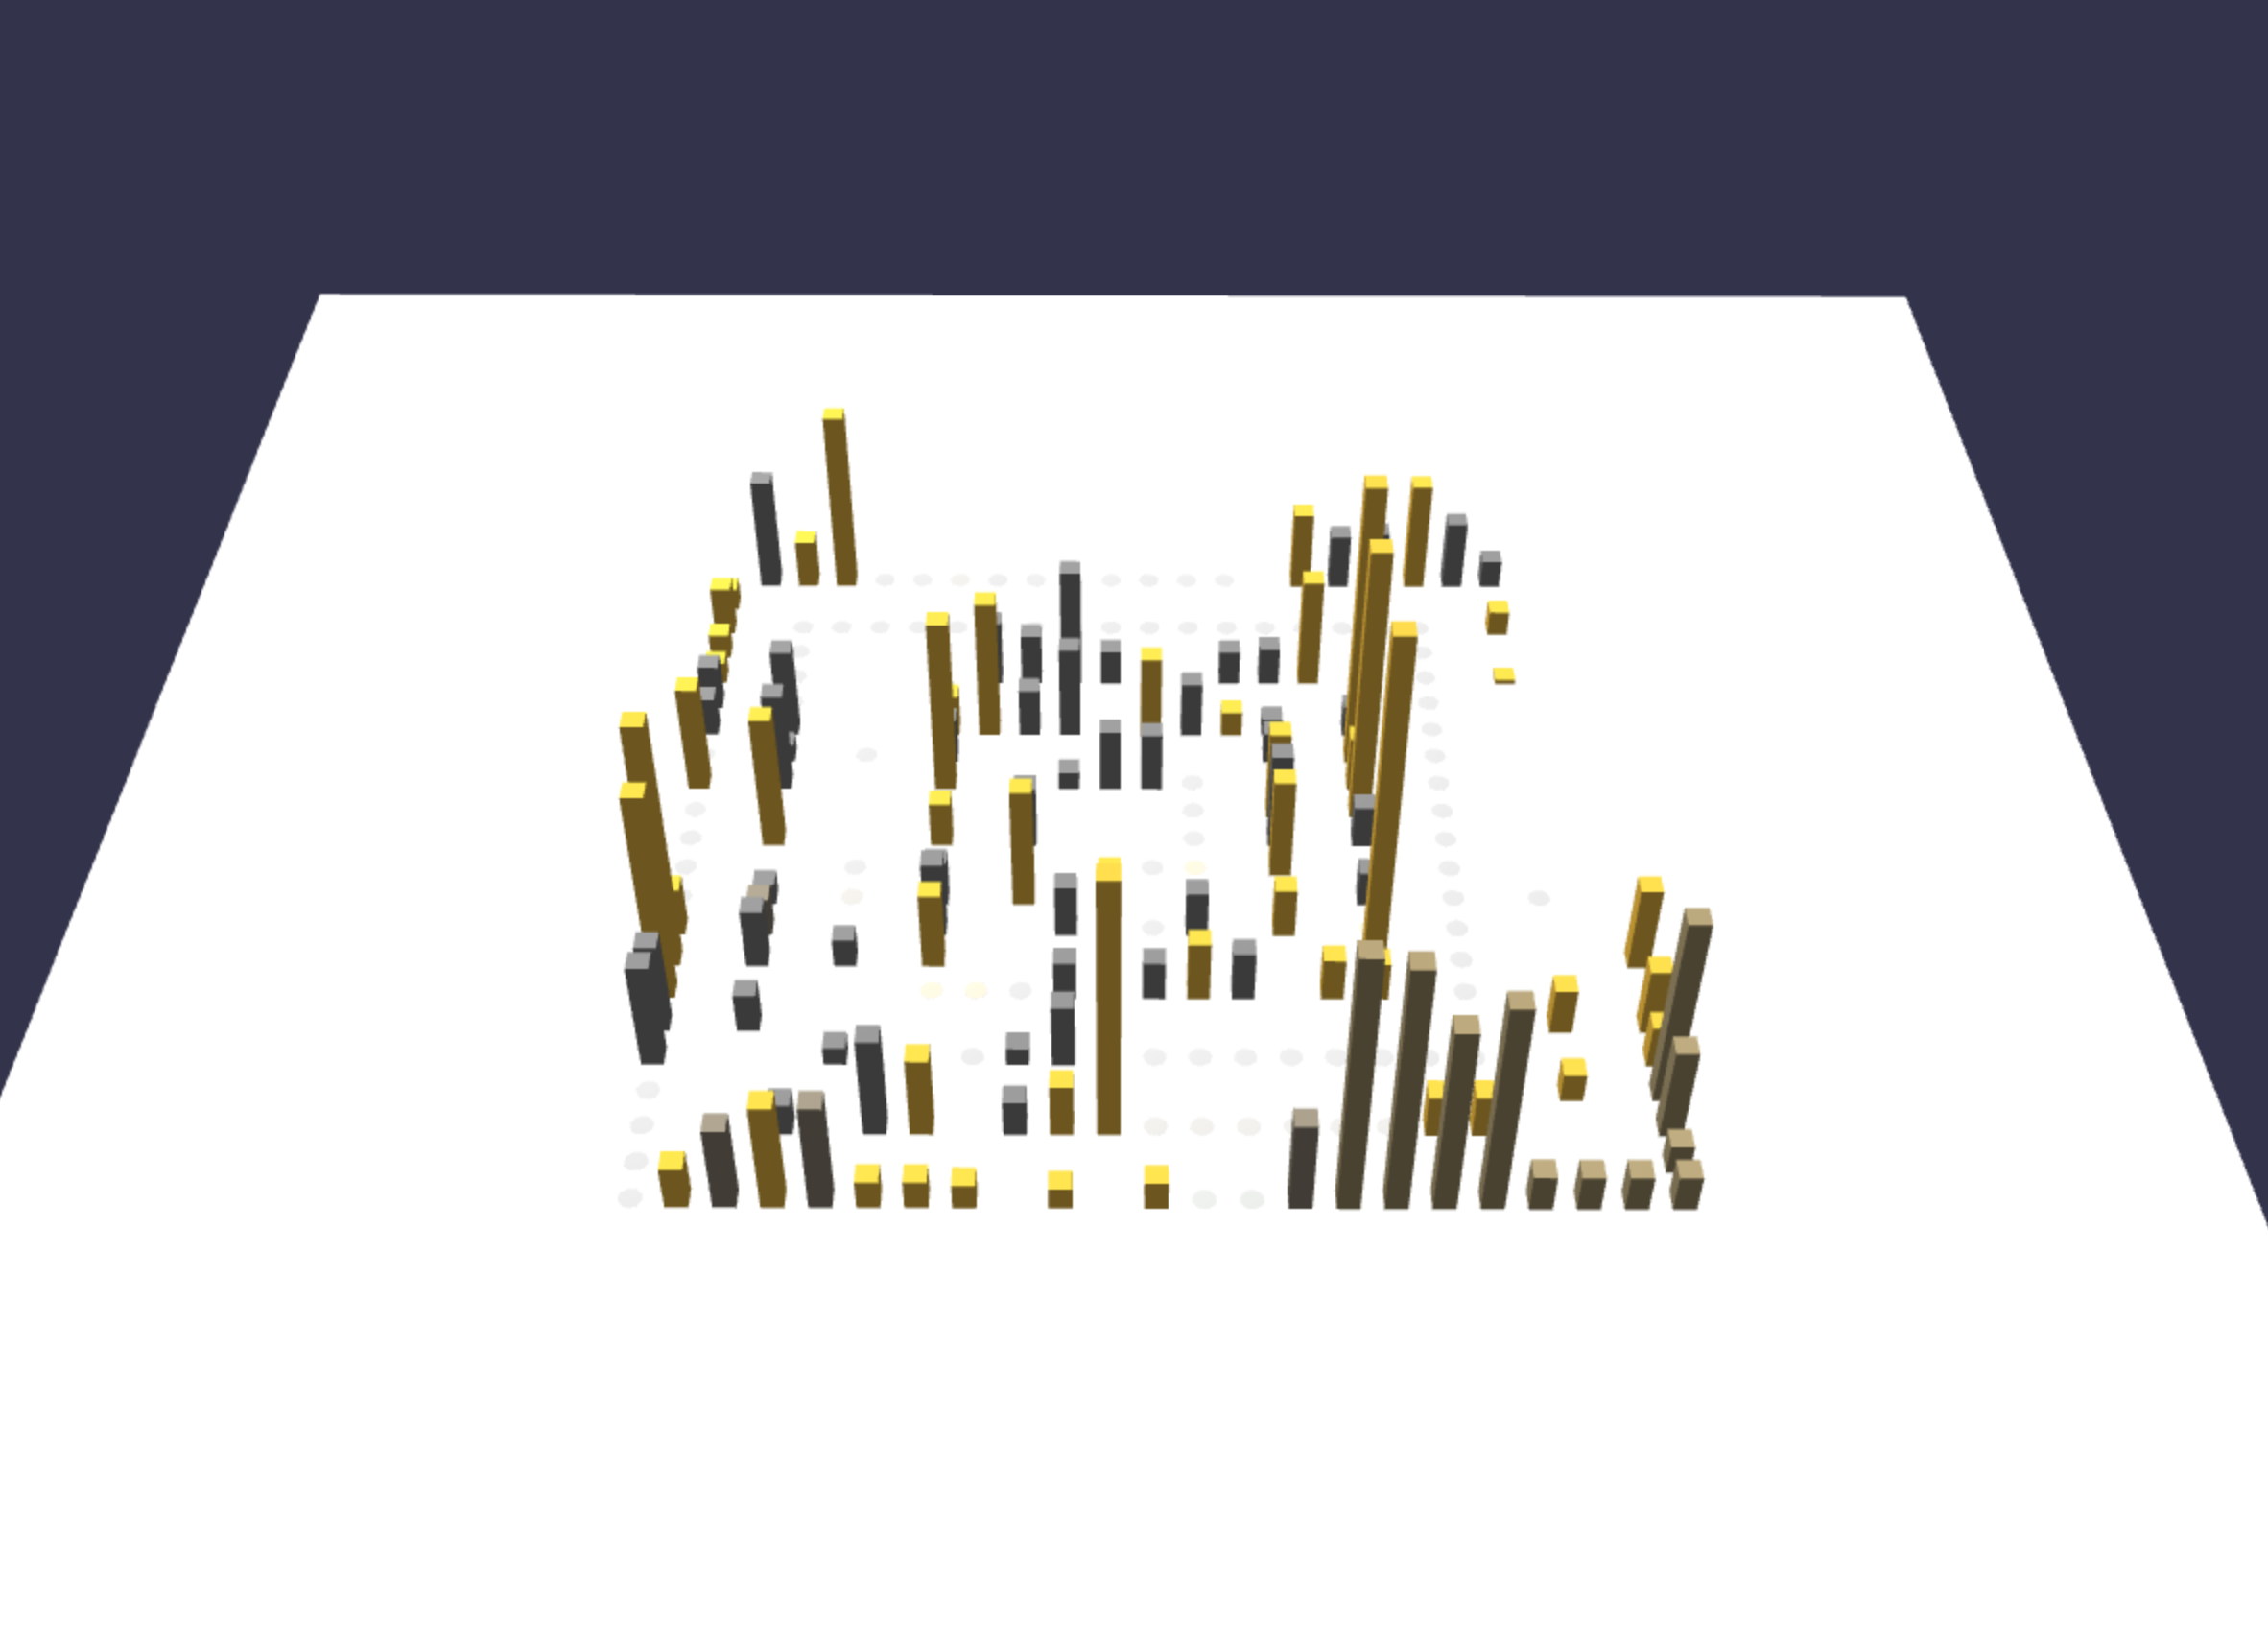
\includegraphics[width=\linewidth]{JetUML_V3S2.png}
        \caption{Year 2} 
        \label{fig:JetUML_V3S2}
    \end{subfigure}
    
    \medskip
    \begin{subfigure}{0.48\textwidth}
        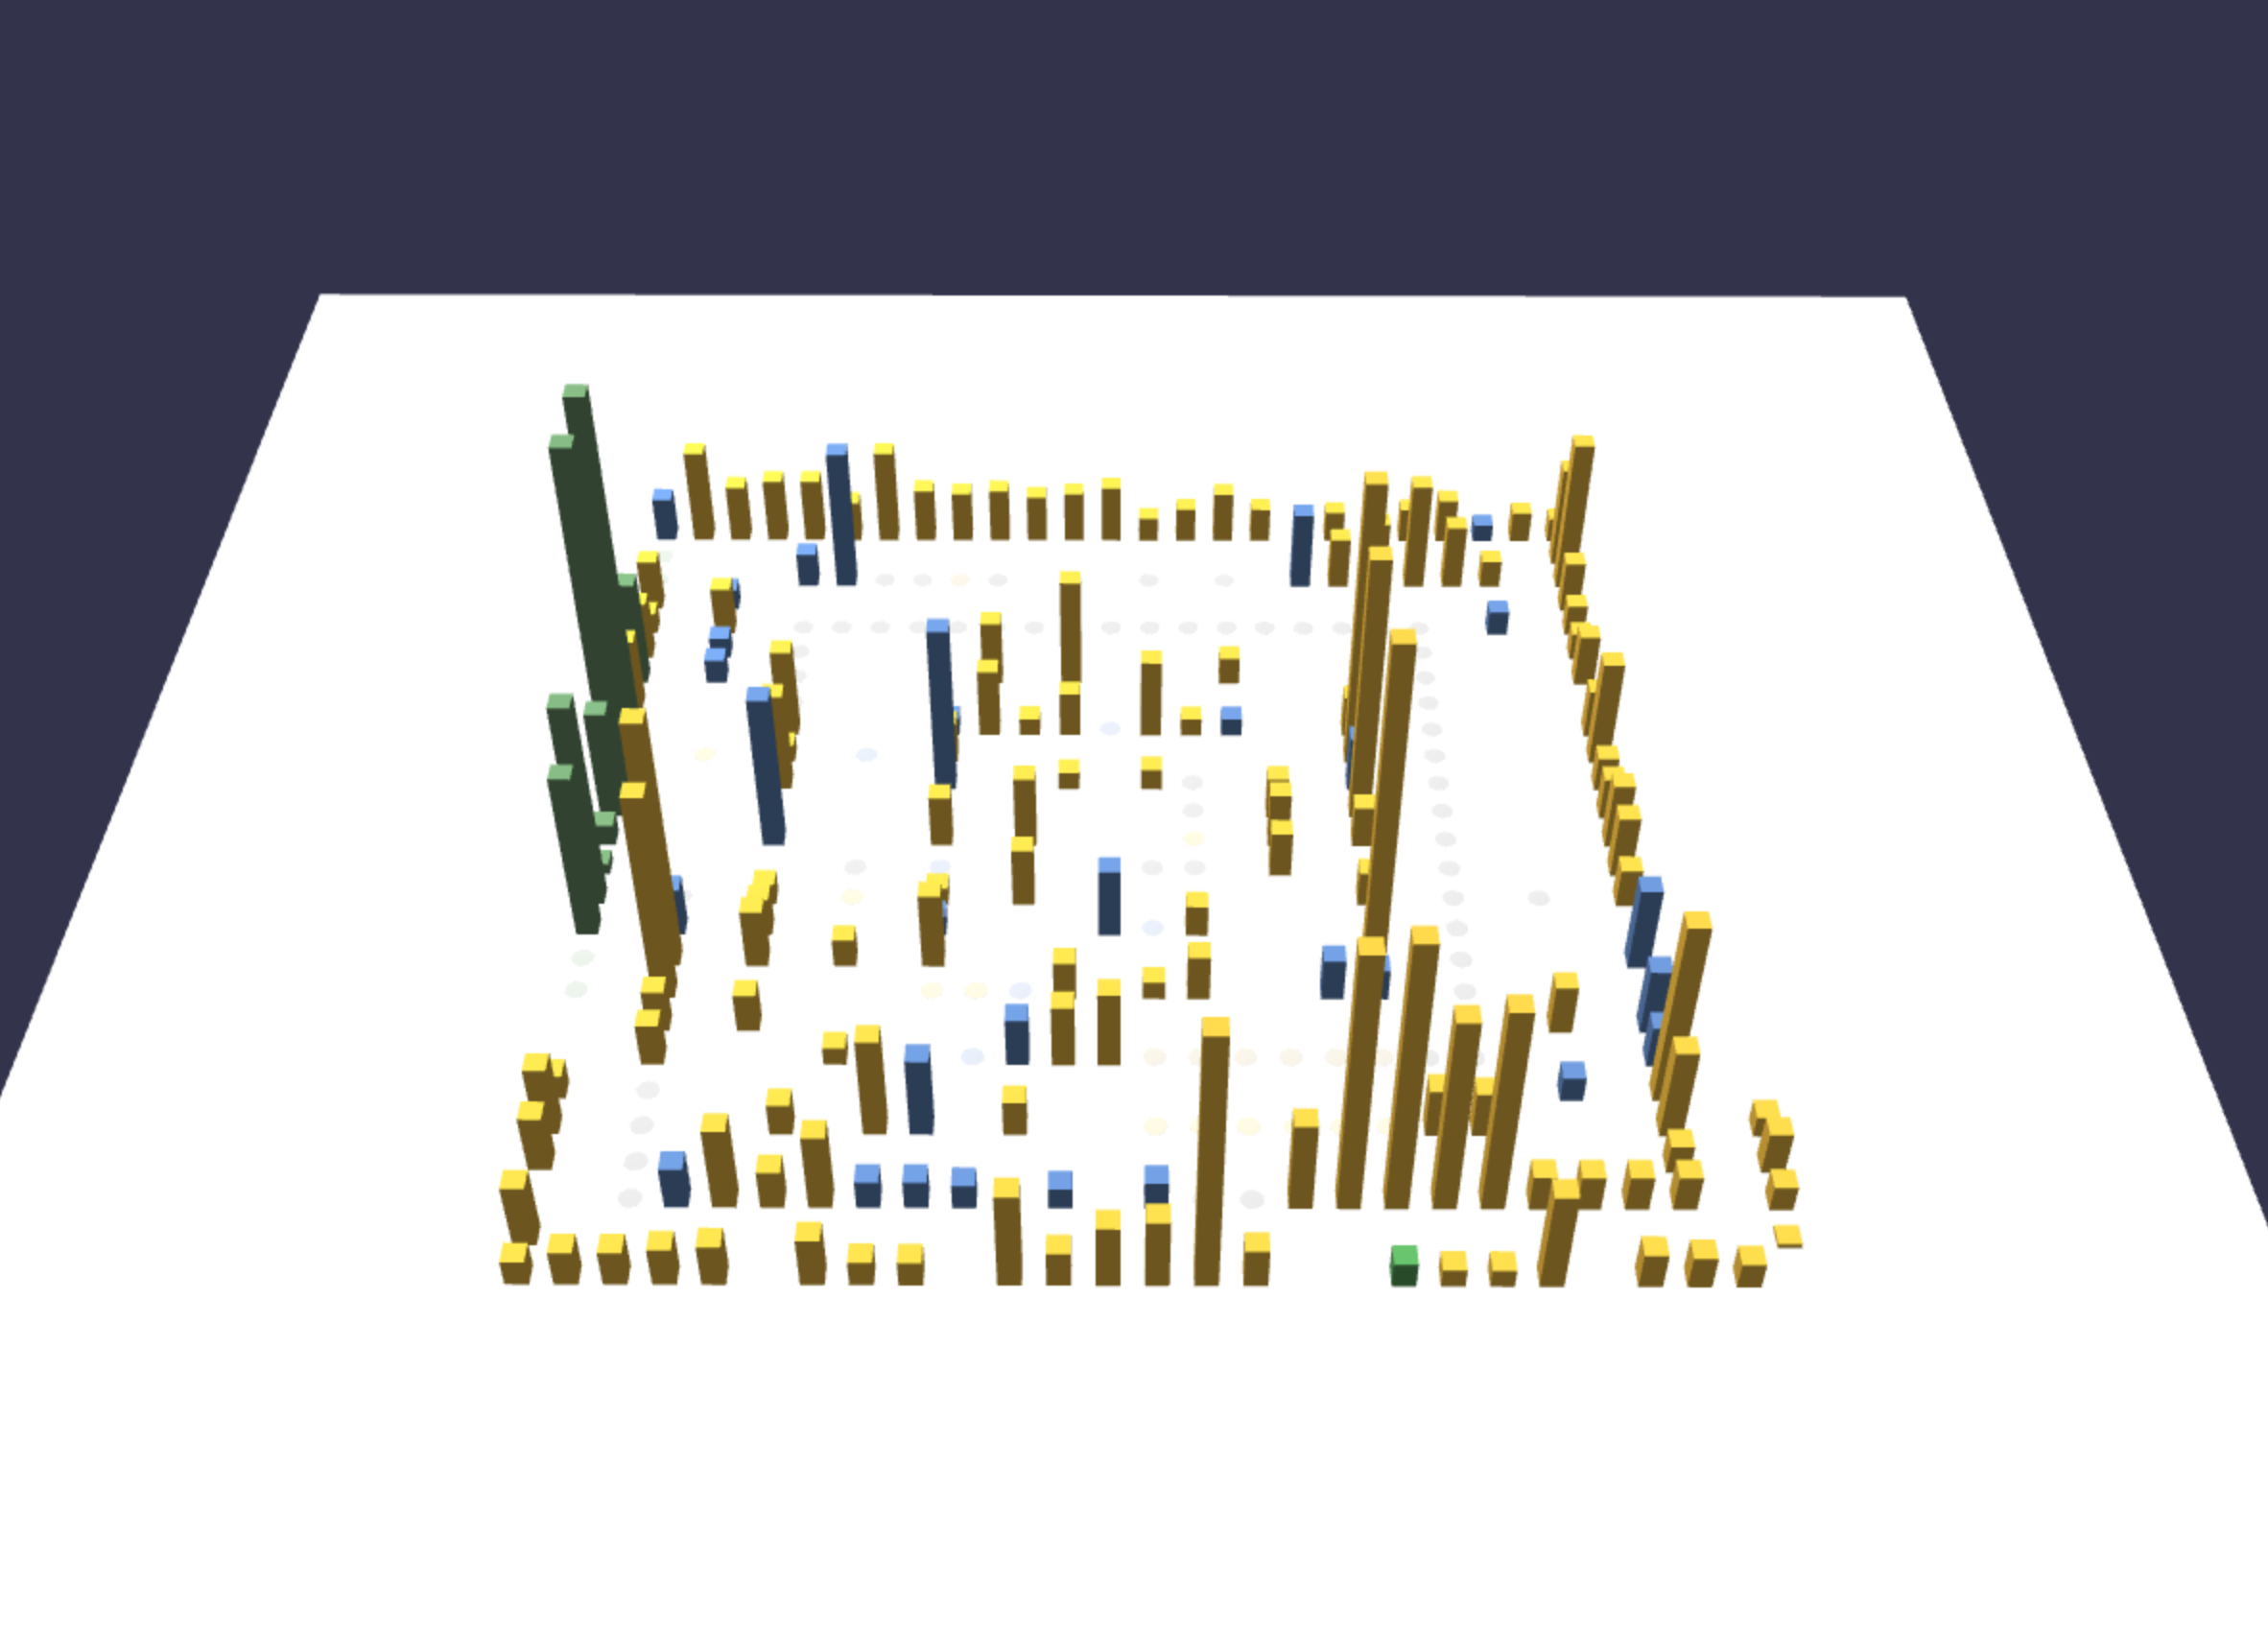
\includegraphics[width=\linewidth]{JetUML_V3S3.png}
        \caption{Year 3} 
        \label{fig:JetUML_V3S3}
    \end{subfigure}\hspace*{\fill}
    \begin{subfigure}{0.48\textwidth}
        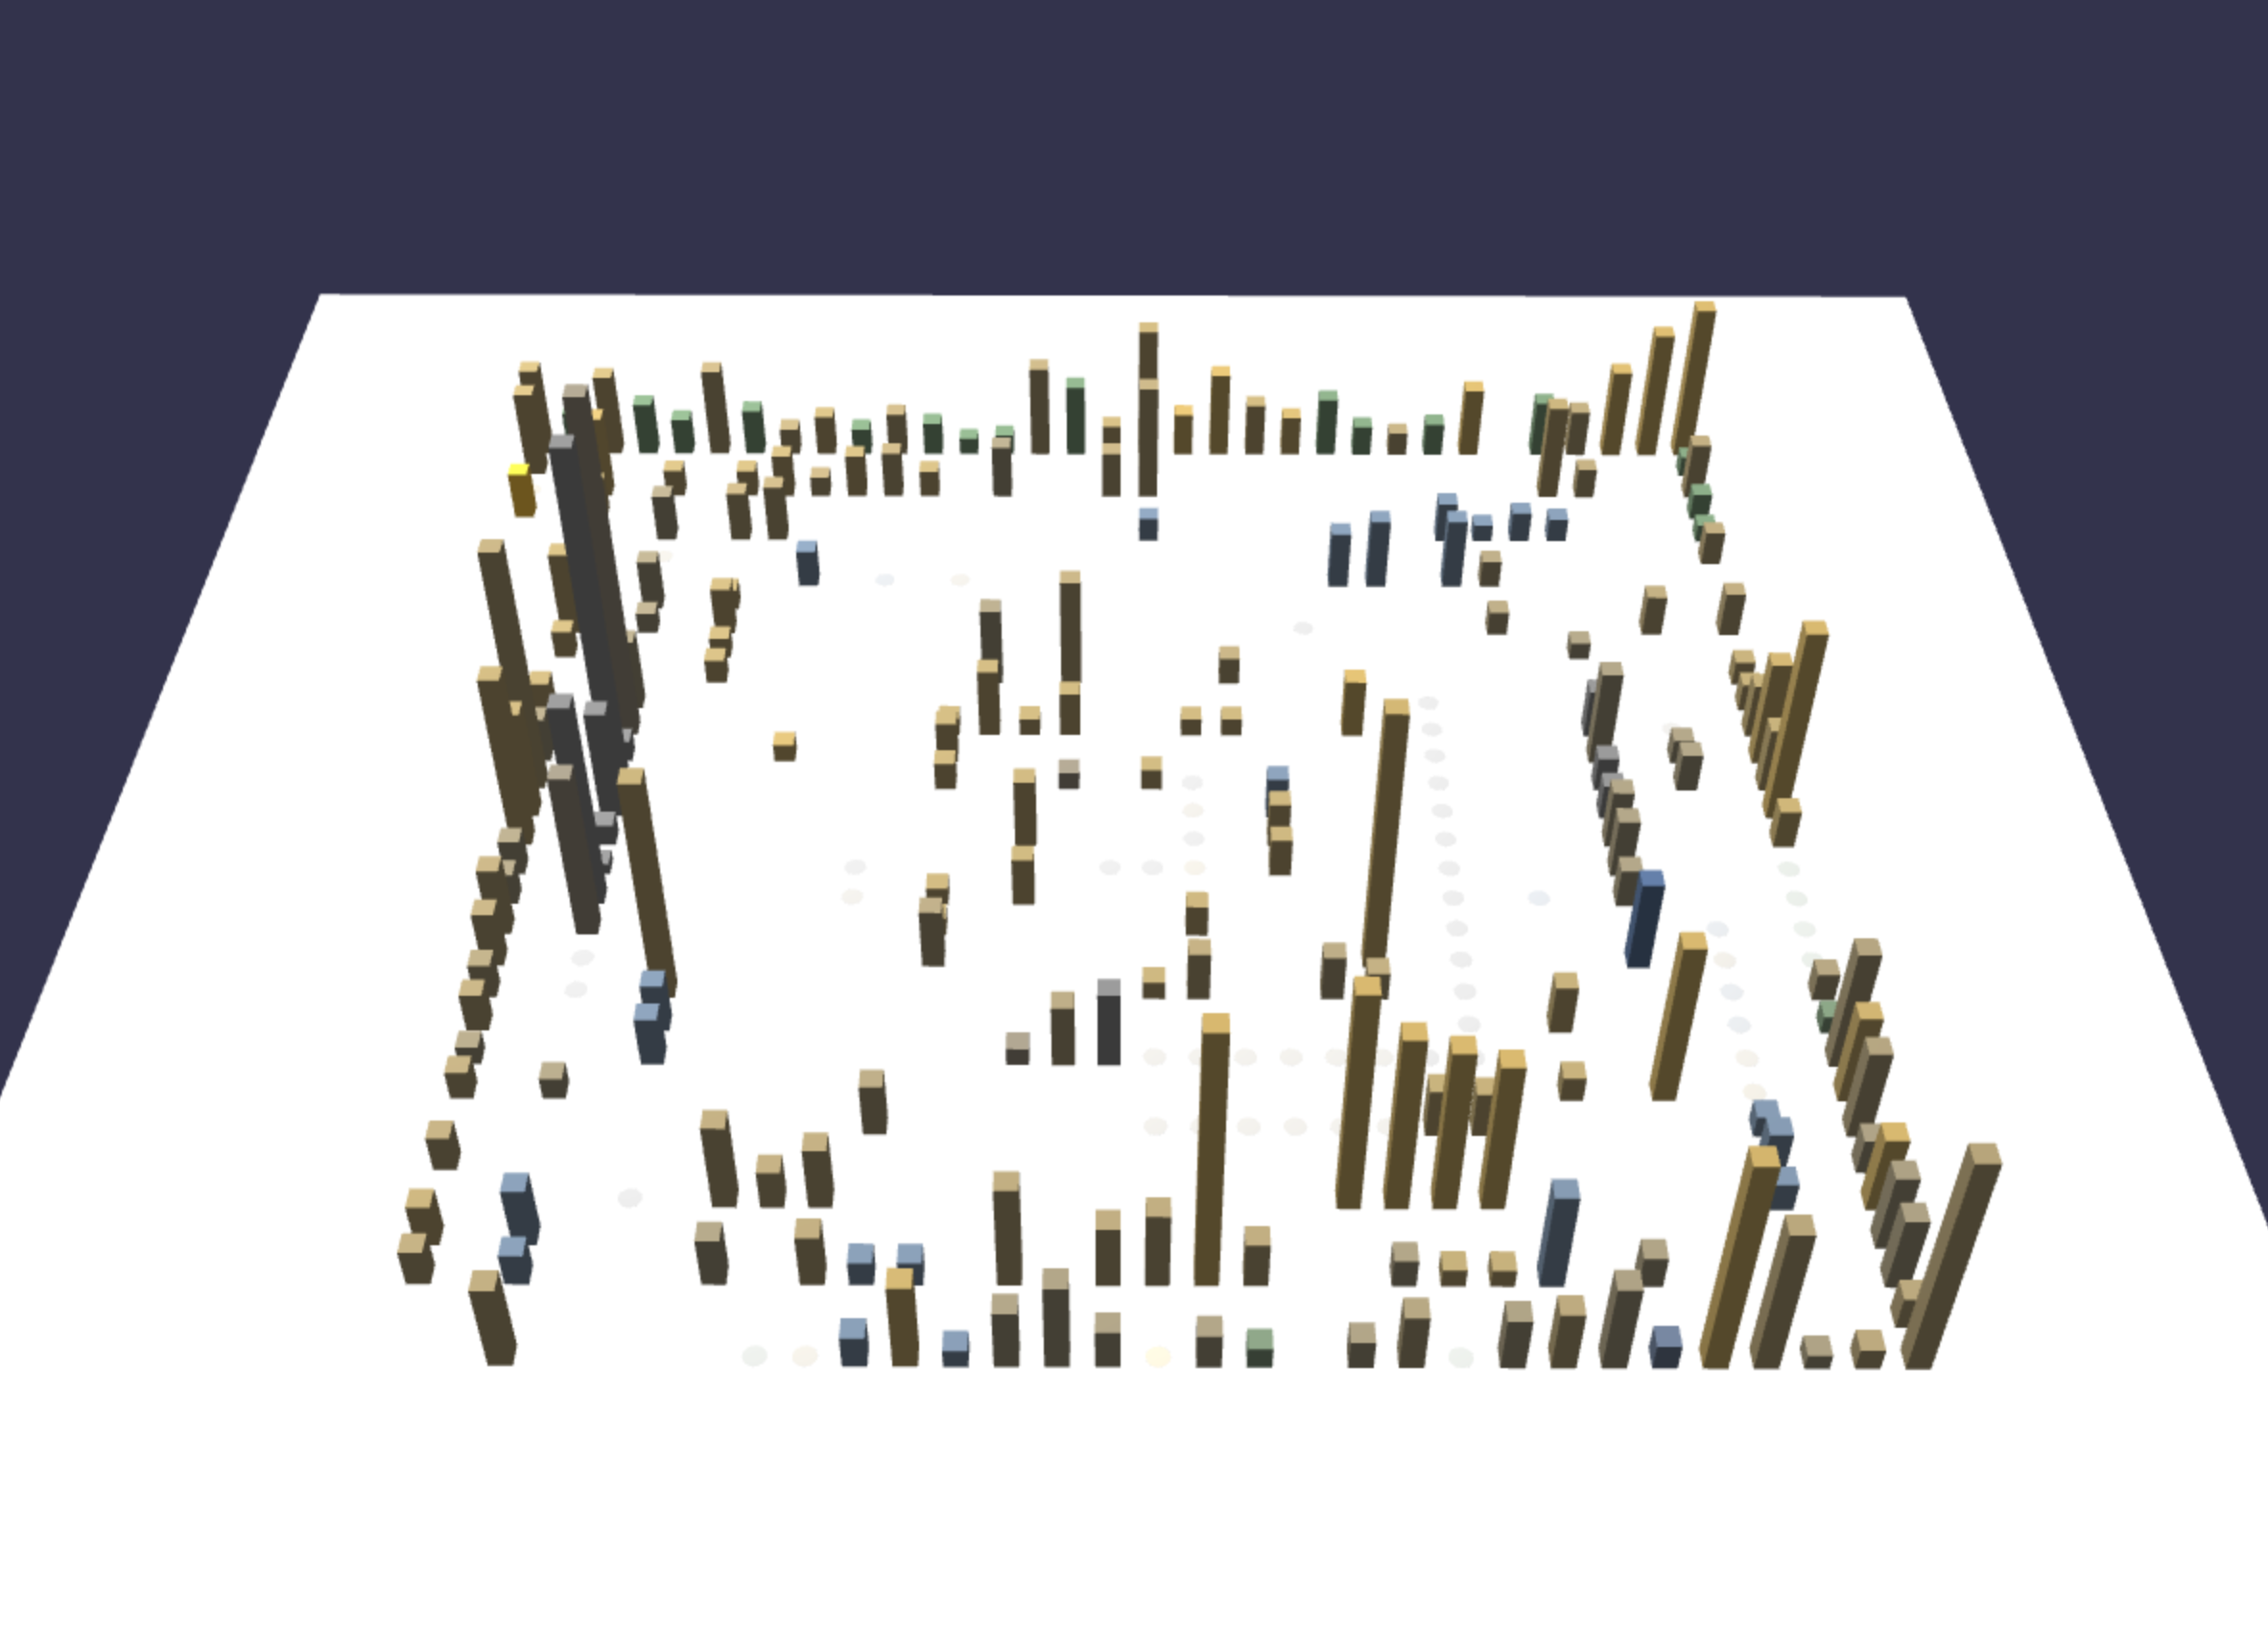
\includegraphics[width=\linewidth]{JetUML_V3S4.png}
        \caption{Year 4} 
        \label{fig:JetUML_V3S4}
    \end{subfigure}
        
    \caption{Evolution of JetUML} 
    \label{fig:JetUML_V3}
\end{figure}

\begin{figure}[ht]    \ContinuedFloat
    \begin{subfigure}{0.48\textwidth}
        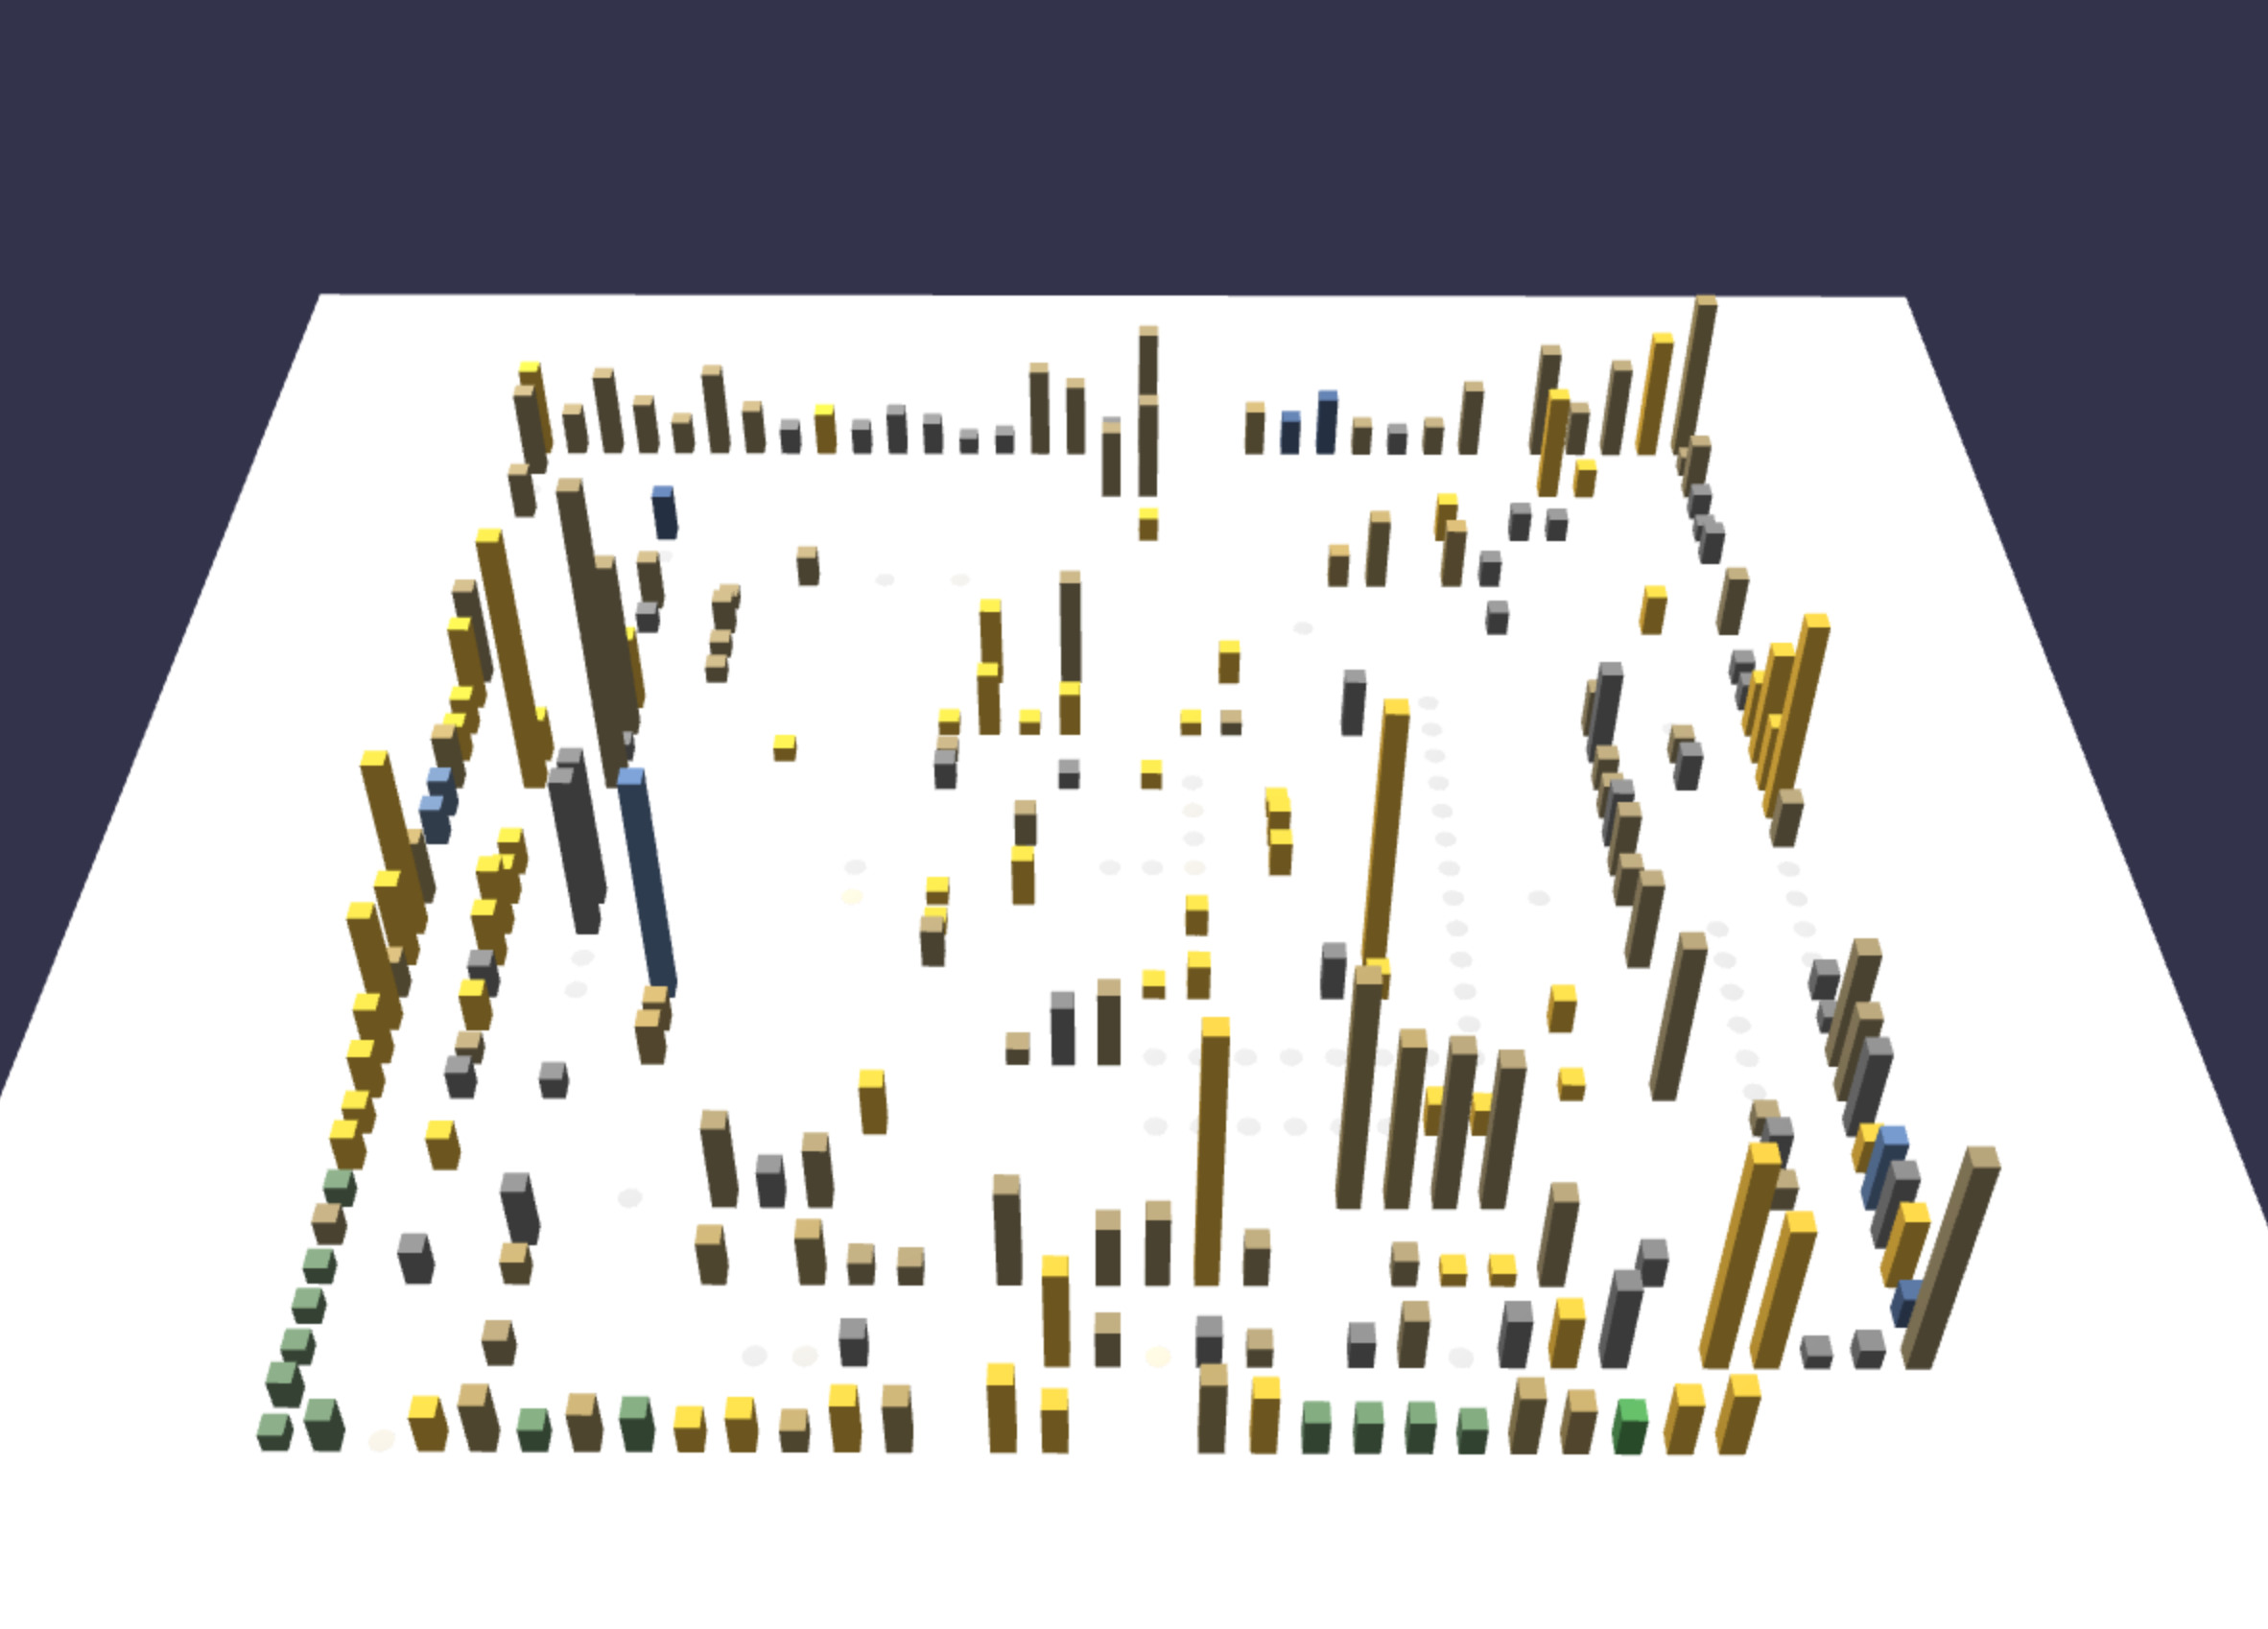
\includegraphics[width=\linewidth]{JetUML_V3S5.png}
        \caption{Year 5} 
        \label{fig:JetUML_V3S5}
    \end{subfigure}\hspace*{\fill}
    \begin{subfigure}{0.48\textwidth}
        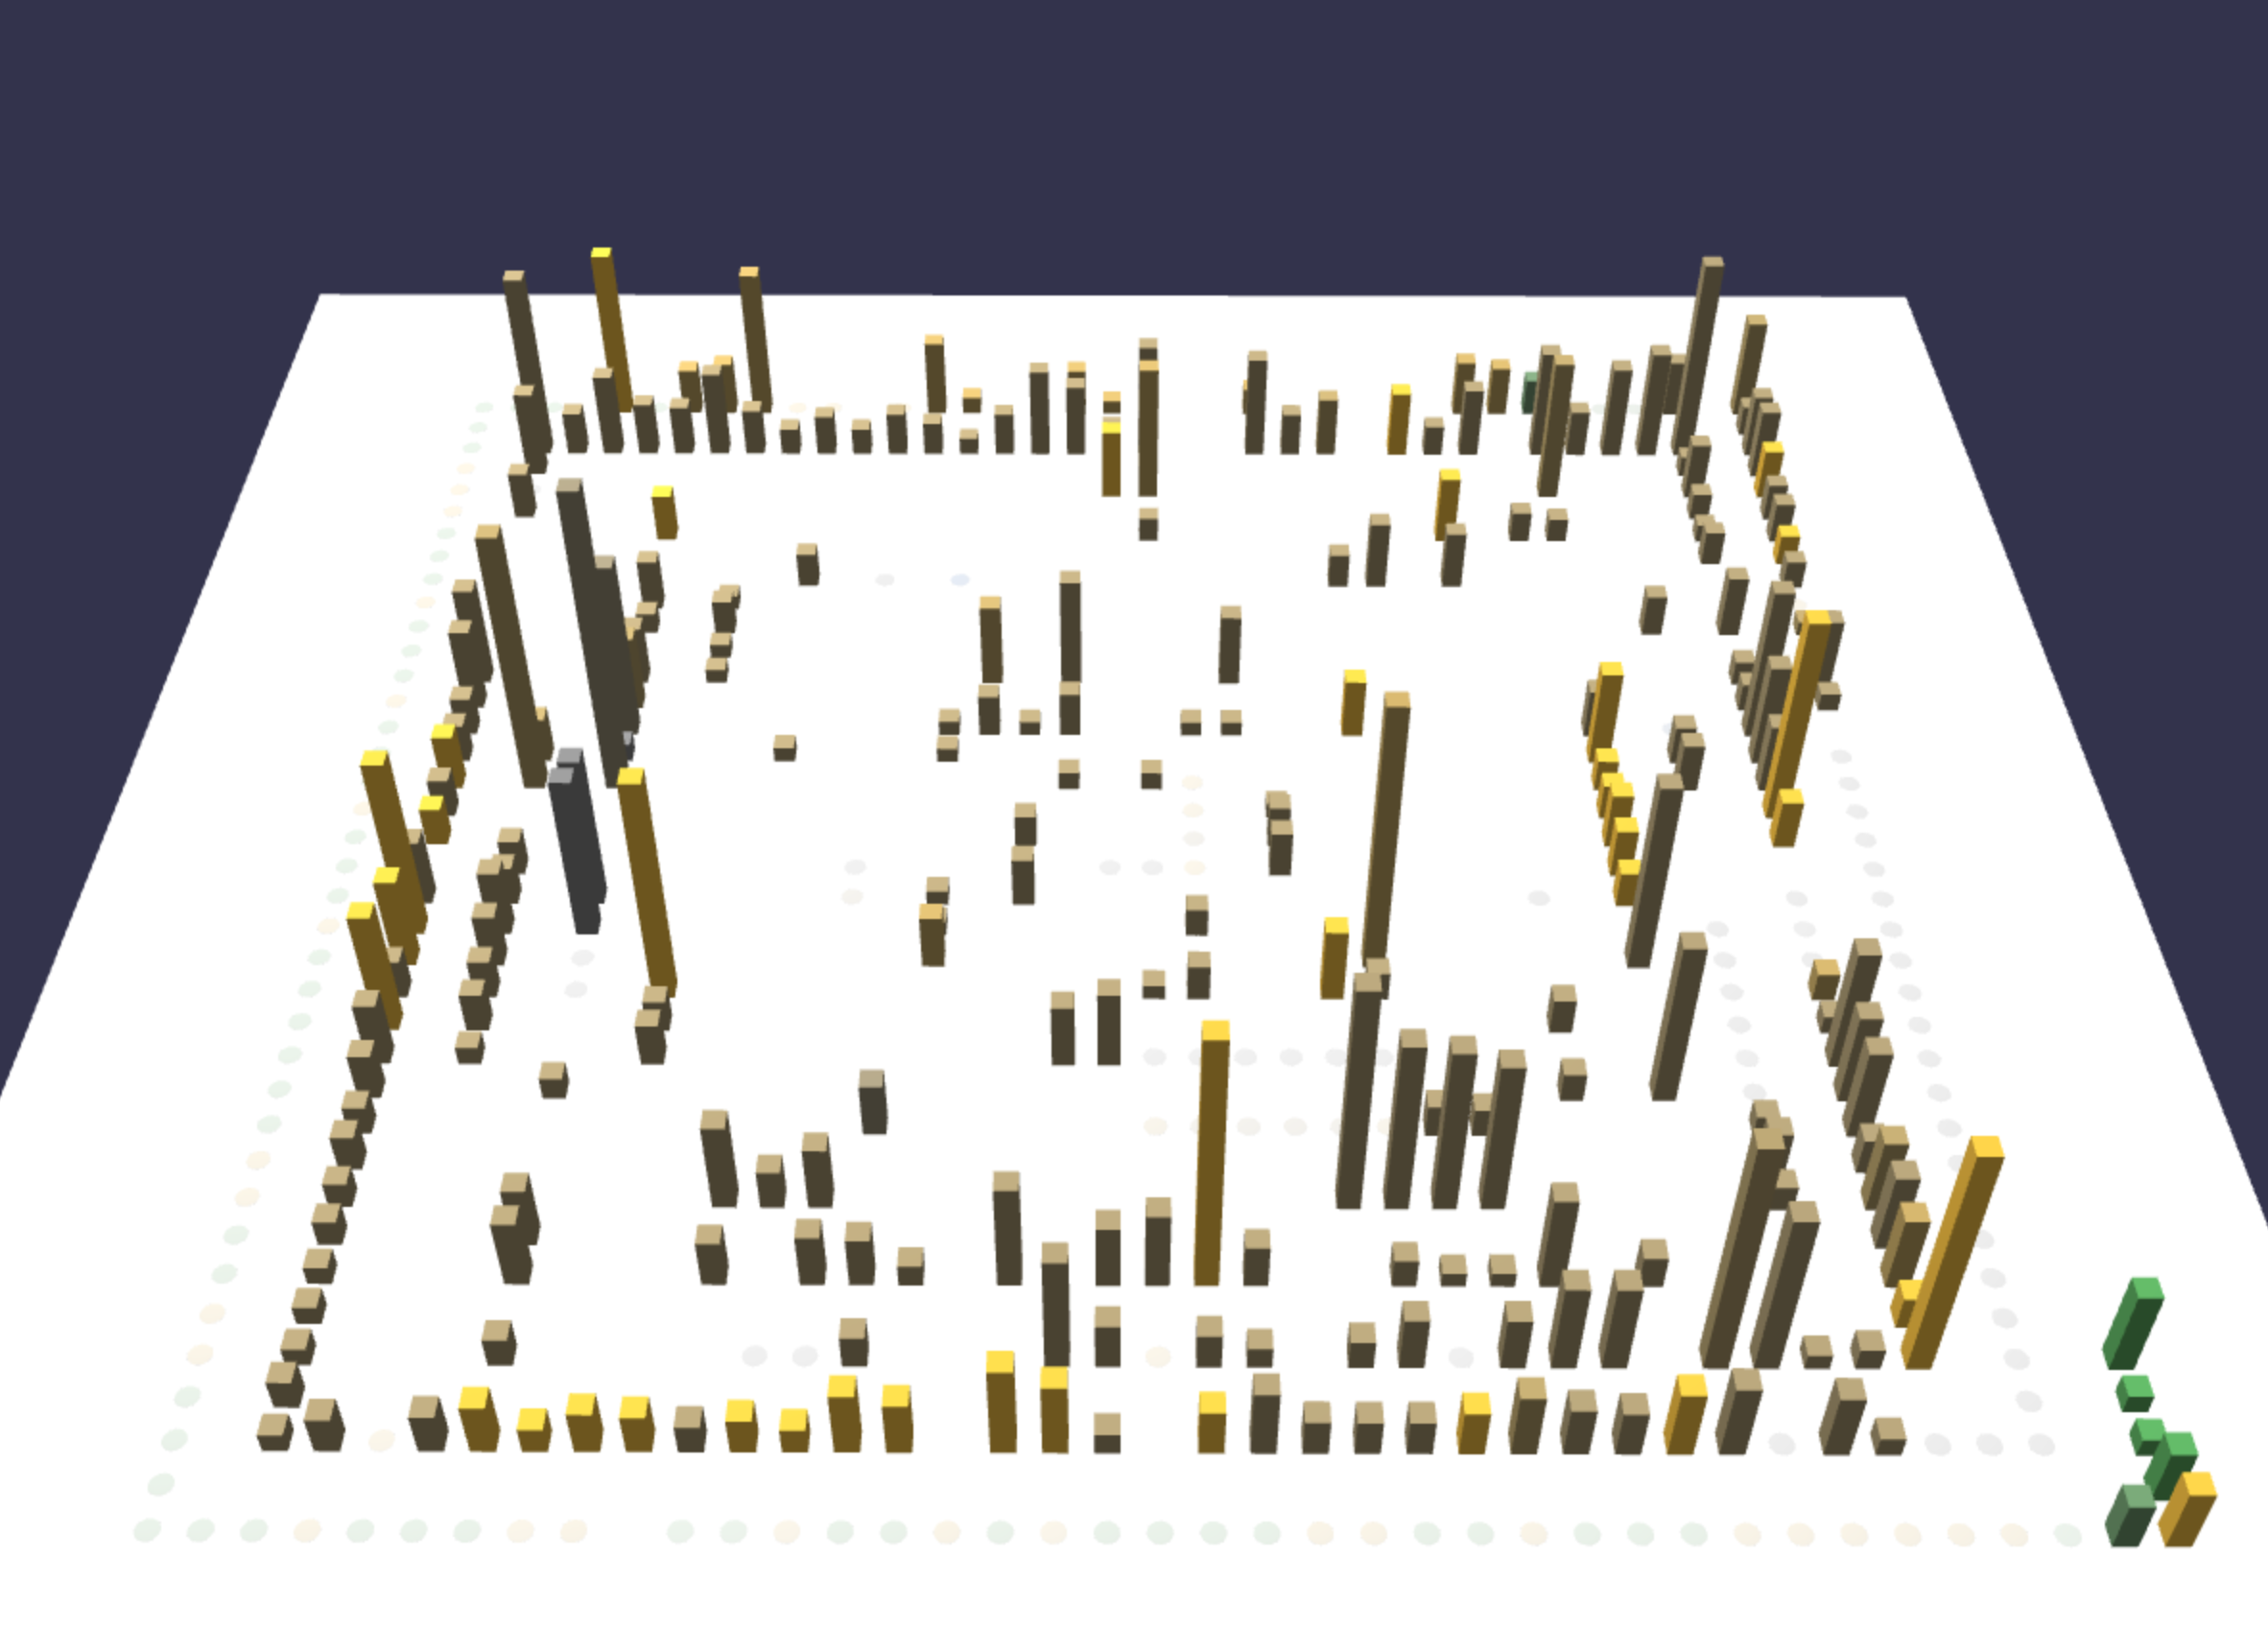
\includegraphics[width=\linewidth]{JetUML_V3S6.png}
        \caption{Year 6} 
        \label{fig:JetUML_V3S6}
    \end{subfigure}

    \medskip
    \begin{subfigure}{0.48\textwidth}
        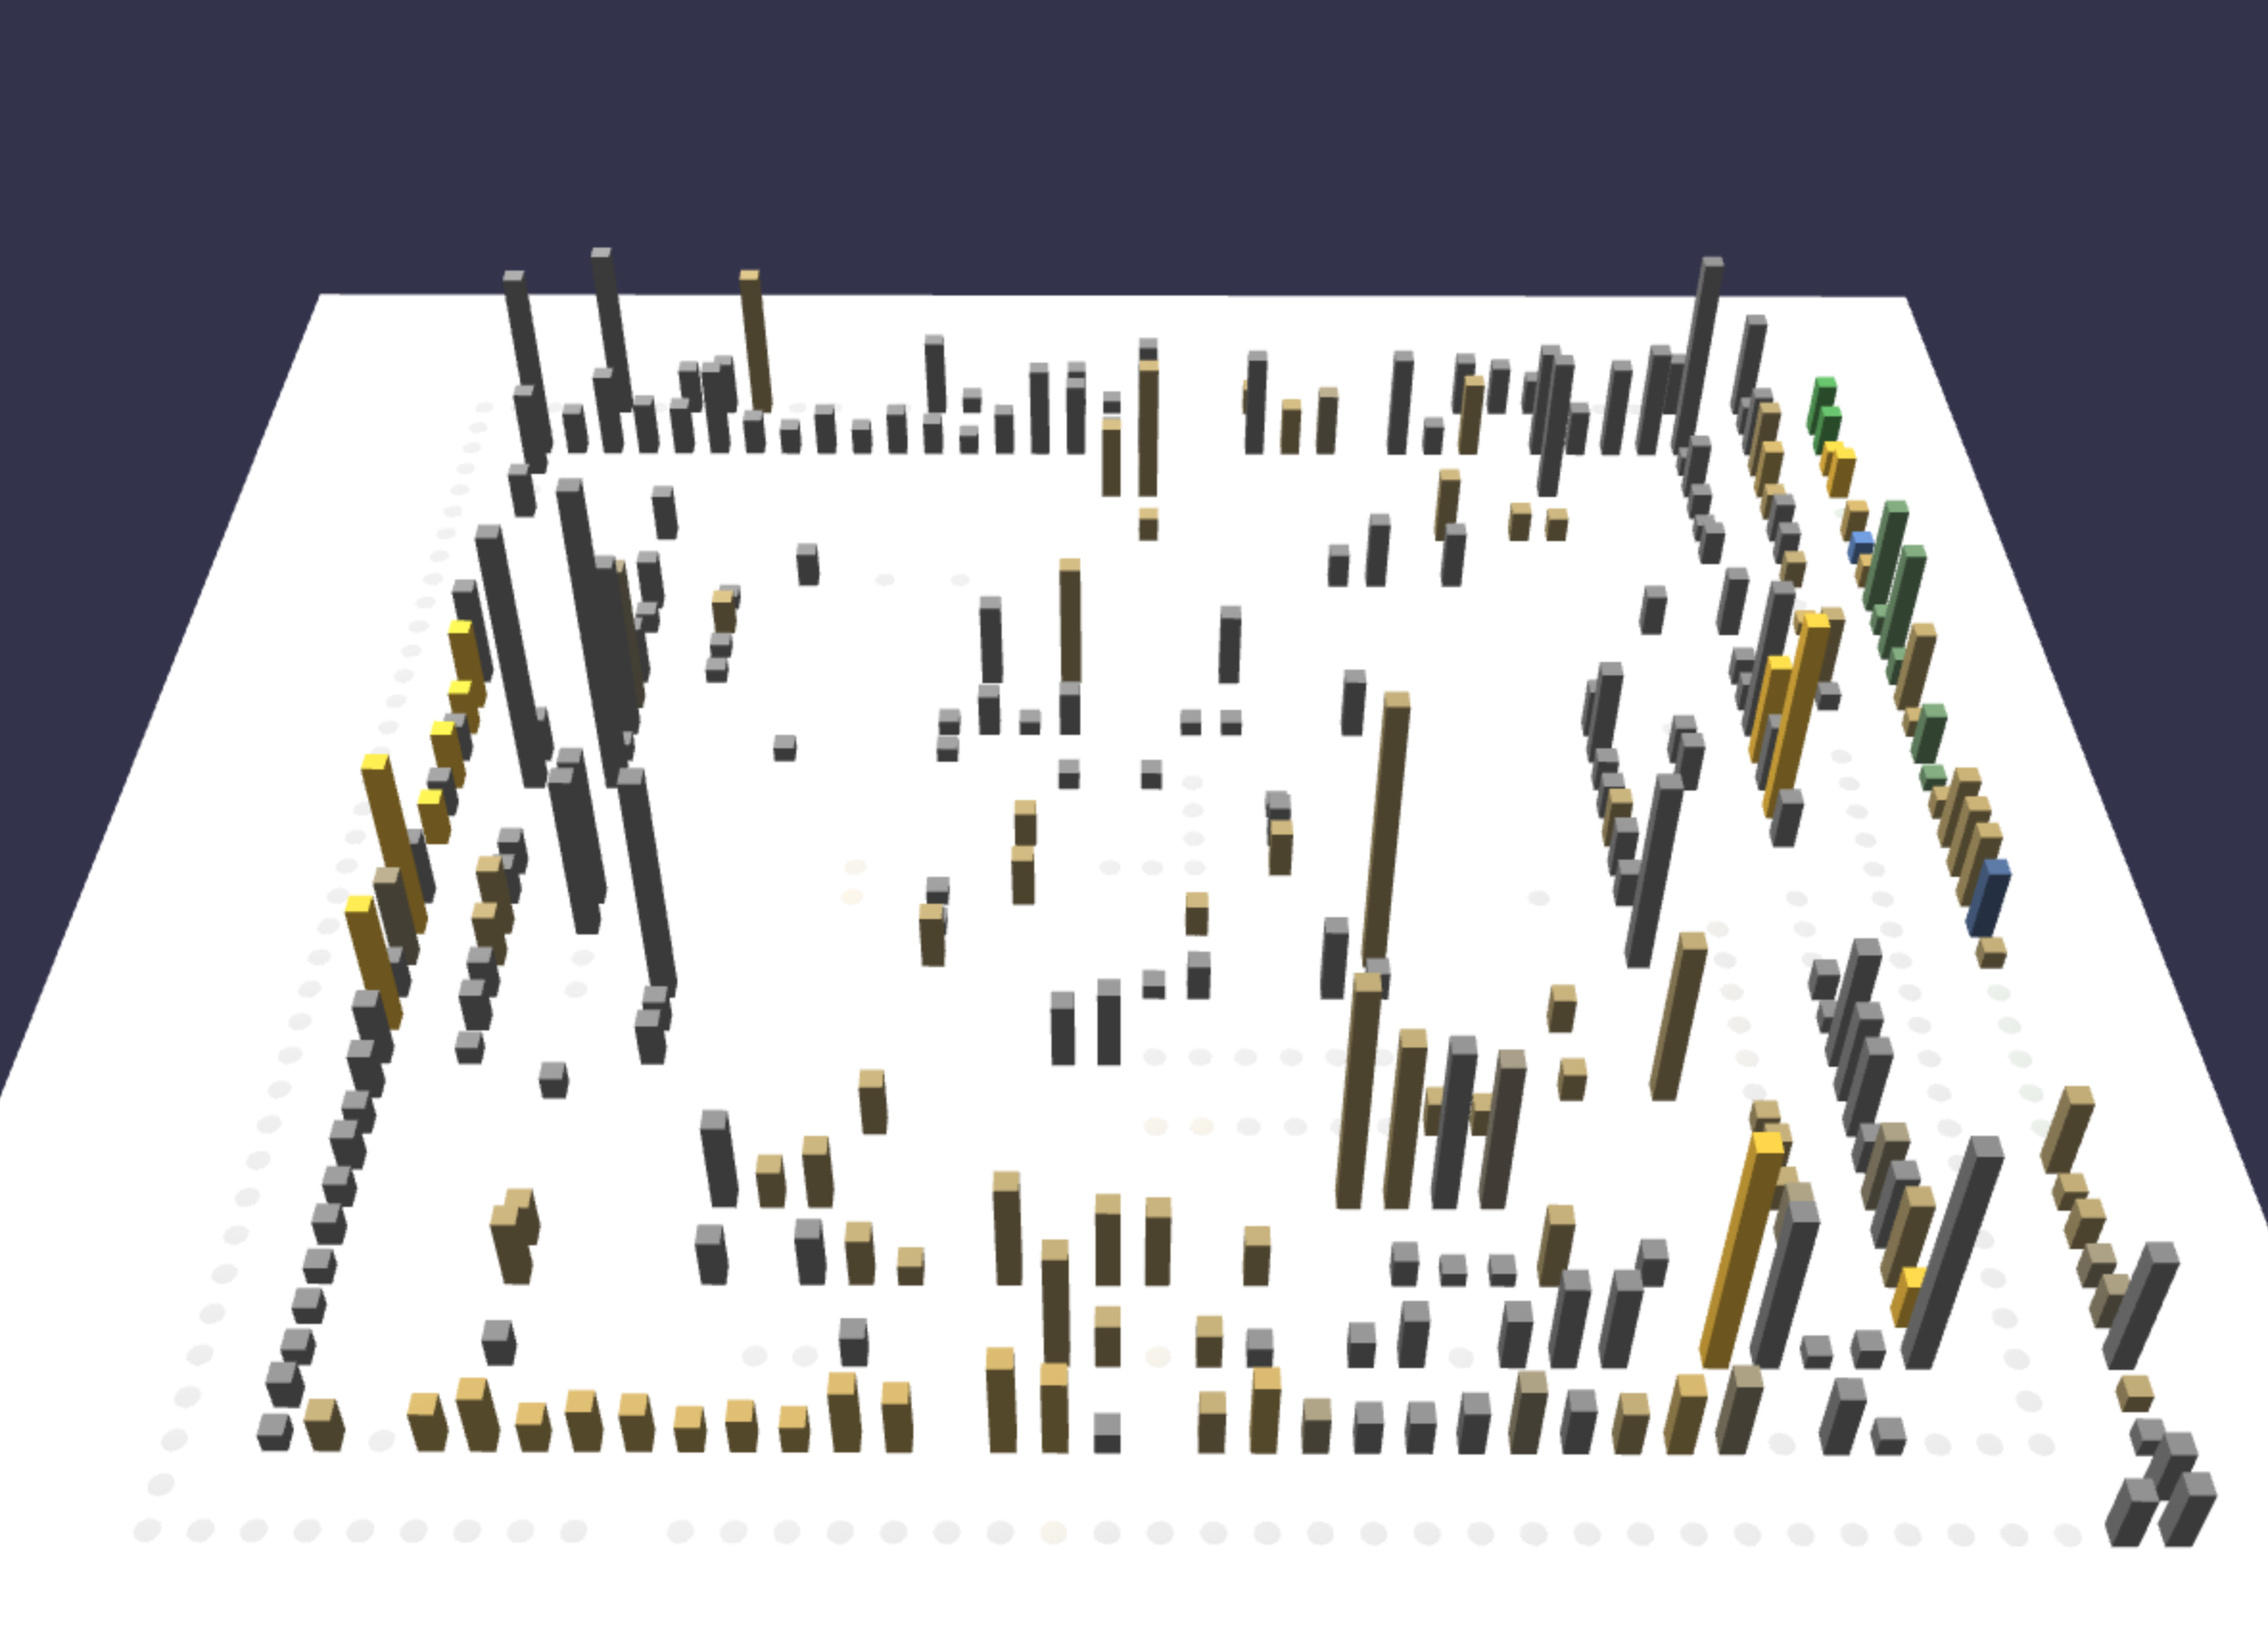
\includegraphics[width=\linewidth]{JetUML_V3S7.png}
        \caption{Year 7} 
        \label{fig:JetUML_V3S7}
    \end{subfigure}\hspace*{\fill}
    \begin{subfigure}{0.48\textwidth}
        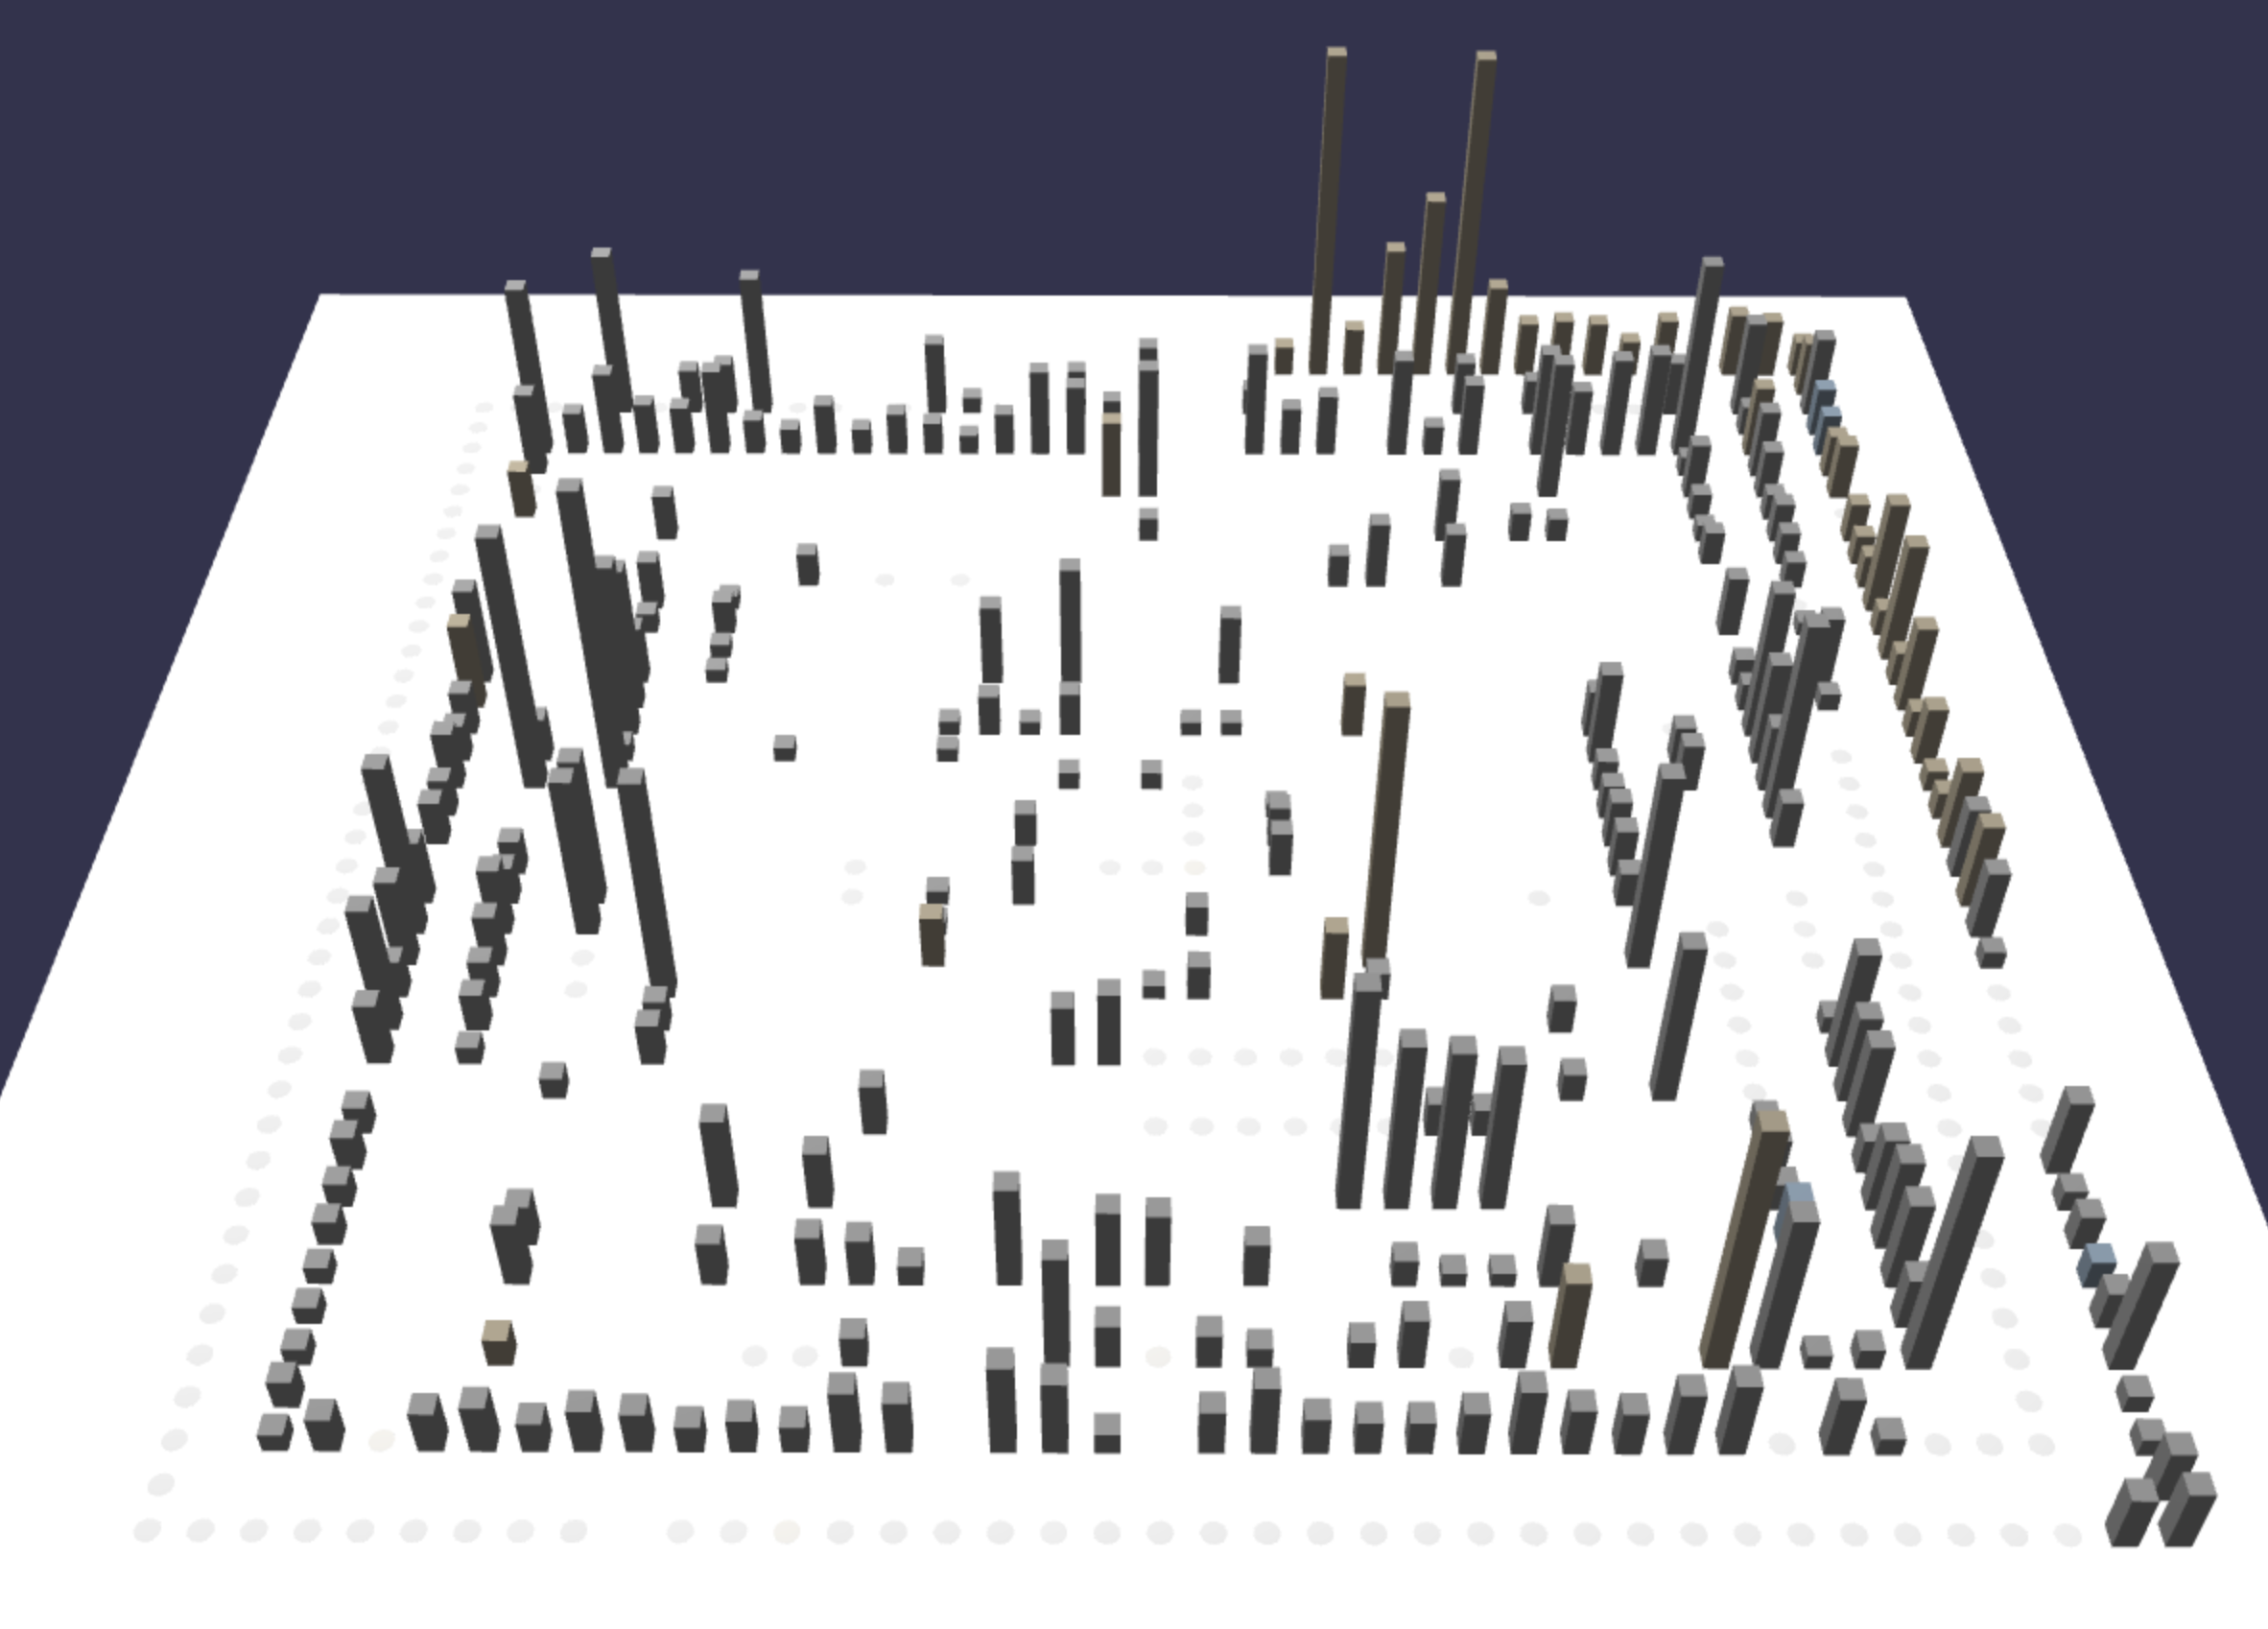
\includegraphics[width=\linewidth]{JetUML_V3S8.png}
        \caption{Year 8 (last)} 
        \label{fig:JetUML_V3S8}
    \end{subfigure}
    
    \caption{Evolution of JetUML} 
    \label{fig:JetUML_V3_F1}
\end{figure}

% -------------------------------------------
% argouml
% FileHistories: 11129 
% ProjectVersions: 16672 
% FileVersions: 91667 
% First Version: 
% 	 hash: 6ef818a48b453627fd282971f3f9a28e28f54390 
% 	 date: Mon Jan 26 23:19:17 CET 1998 
% Last Version: 
% 	 hash: 3ddc7f94d83c4e2f439ca6fc0fe787616a1900a9 
% 	 date: Sat May 29 23:18:44 CEST 2021 
% Diff: {DAYS=128, HOURS=22, MINUTES=59, SECONDS=27, MILLISECONDS=0, MICROSECONDS=0, NANOSECONDS=0, YEARS=23}
% -------------------------------------------
\clearpage
\section{ArgoUML – 23 Years of History}
This section analyzes ArgoUML, a leading open source UML modeling tool. 
It is hosted on GitHub.\footnote{\url{https://github.com/argouml-tigris-org/argouml}}
This repository was created in January 1998, converted from CVS to Subversion in 2006, and finally moved to git in 2019.
It has more than 23 years of history. 
Our analysis considered 16,672 commits, 11,129 FileHistories, and more than 90K FileVersions. 

\bigbreak
%\subsection{View 4}
\label{subsec:view4}
\textbf{Visualization goal:}
This visualization aims to understand how the repository evolved through these 23 years. Therefore we adopt a commit grouping strategy based on a time window of one year and an aging strategy of one month with a total of 12 steps. Hence, grey entities represent files that have not been updated for more than 12 months. 


View specification adopted: 
\begin{itemize}
    \item \texttt{versionGroupingStrategy}: timestamp.
    \item \texttt{versionGroupingChunkSize}: 31,556,926 (1 year). 
    \item \texttt{colorPalette}: default.
    \item \texttt{agingGroupingStrategy}: timestamp.
    \item \texttt{agingStepSize}: 2,629,743 (1 month).
    \item \texttt{agingSteps}: 12 steps.
    \item \texttt{mapperMetricName}: SIZE. 
    \item \texttt{fileTypeShape}: all BOX. 
    \item \texttt{fileTypeOpacity}: all 1. 
\end{itemize}

\textbf{Results:}
Here we present an interesting summary of ArgoUML's evolution. The full evolution is depicted in  \autoref{app:ArgoUML_Evolution}. \autoref{fig:JetUML_V3} shows the hotspots during the system's evolution. \autoref{fig:ArgoUML_V3_S1} shows the system's state after the first year of development. As we can notice, almost all the entities have a color different than gray. This means they were updated between April 1998 and January 1999 otherwise they should be darker or gray. The size of the system was constantly increasing in 2003. As \autoref{fig:ArgoUML_V3_S2} shows, the system's core was entirely rewritten. Three years later it had another important refactoring. As shown in \autoref{fig:ArgoUML_V3_S3} there are empty rings around the center and a bigger size than the previous year. Our interpretation is that an entire set of consequently added files was removed and maybe later added. It is important to underline that these files were deleted, not moved, or renamed because otherwise, SYN would treat them as the same logical entity. The same event happened four years later, when the system became ten years old. 2010 was the last truly active year for the repository as depicted in \autoref{fig:ArgoUML_V3_S5}. Almost all the repository files were modified and we can notice taller entities, meaning that the overall size of the files increased. The system did not grow anymore after that year. Sometimes some files were updated until 2014 when they became almost inactive. In 2019 they made a commit that removed lots of files.\footnote{\url{https://github.com/argouml-tigris-org/argouml/commit/62d5393eeaf08b749b17107faef255a22da55ce5}} As a result, in January 2020, as represented in \autoref{fig:ArgoUML_V3_S6}, the visualization has more blank spots. Since there was no activity, except for a few files, almost all the entities are painted gray. In June 2022, the system is nearly identical to its version in 2020. 

\bigbreak
\textbf{Conclusion:}
The visualization shows the composition of JetUML and its development pace. Thanks to the spiral layout, where entities are added based on their timestamp, we can see that many older files were removed in the final version. They had to be rewritten elsewhere because the system would have fewer features than before. Moreover, thanks to the aging strategy, we observed breaks in the development of the repository. Nonetheless, some of them are not shown in \autoref{fig:ArgoUML_V3}, they can be found in \autoref{app:ArgoUML_Evolution}. The system became almost inactive in 2014. Since that year, most files were never updated. 



\begin{figure}[ht]
    \begin{subfigure}{0.48\textwidth}
        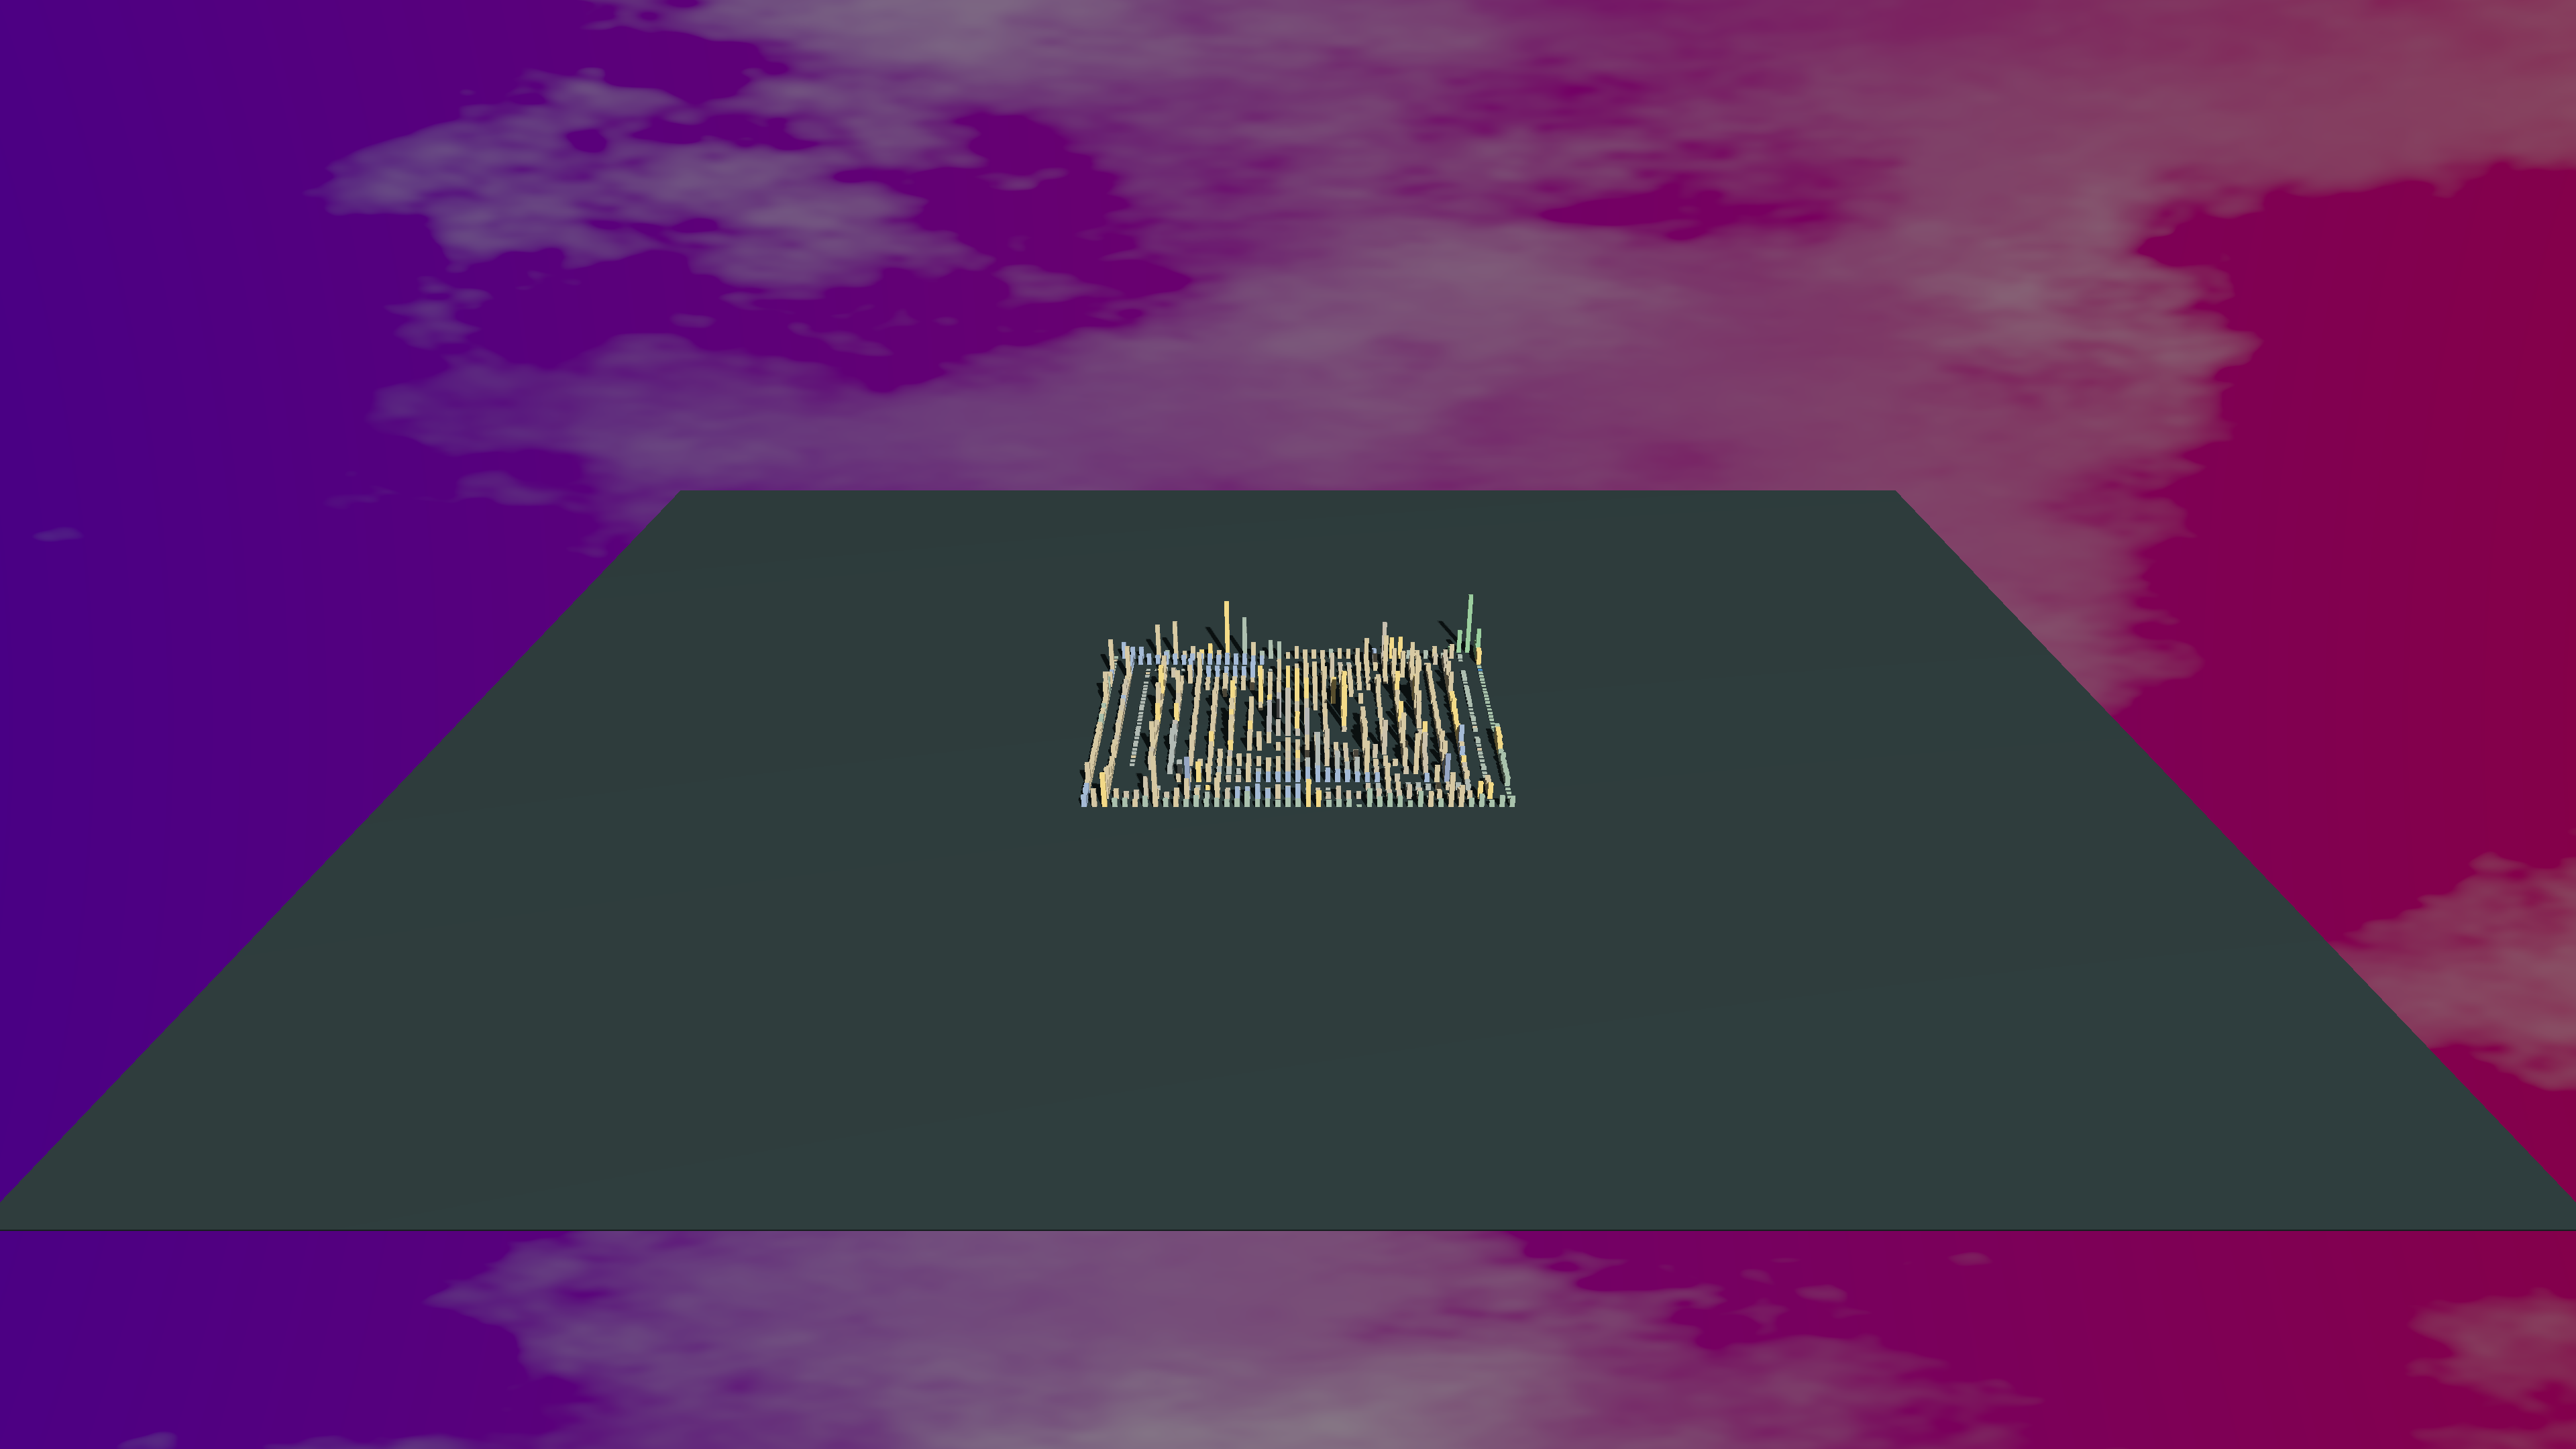
\includegraphics[width=\linewidth]{ArgoUML/Animation001.png}
        \caption{ArgoUML in January 1999 (1 year)} 
        \label{fig:ArgoUML_V3_S1}
    \end{subfigure}\hspace*{\fill}
    \begin{subfigure}{0.48\textwidth}
        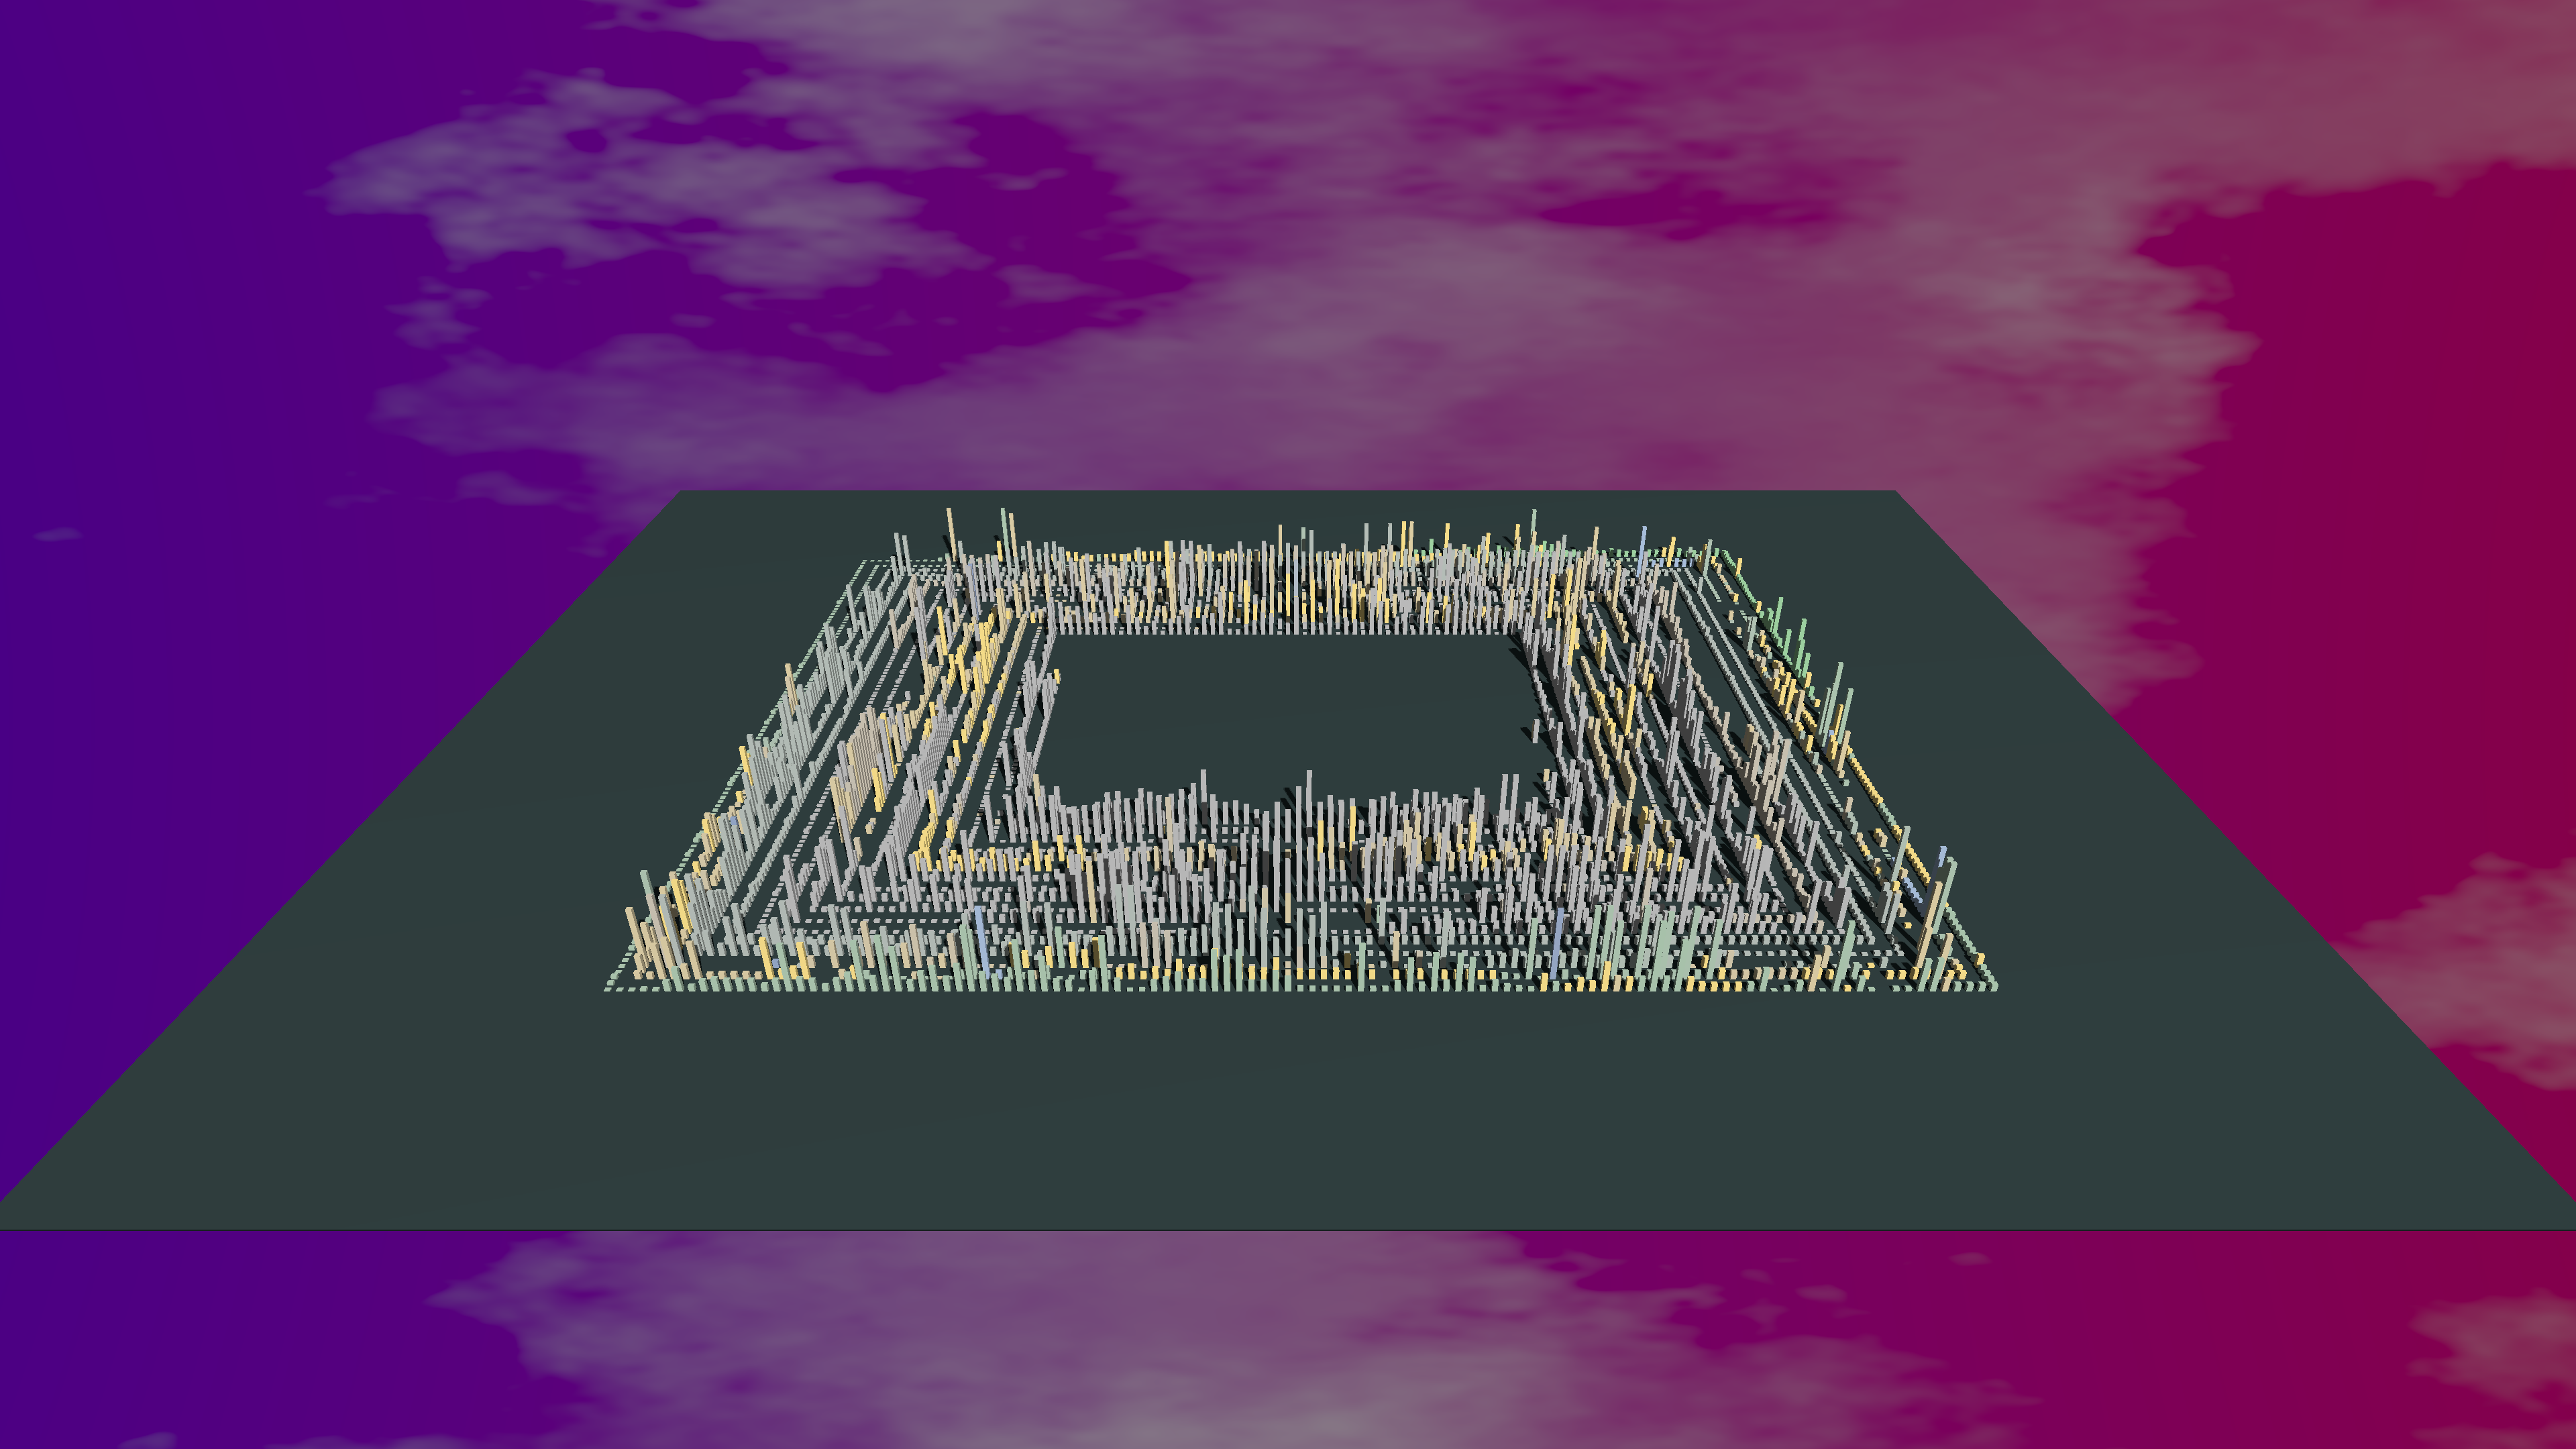
\includegraphics[width=\linewidth]{ArgoUML/Animation005.png}
        \caption{ArgoUML in January 2003 (5 years)} 
        \label{fig:ArgoUML_V3_S2}
    \end{subfigure}
    \medskip
    \begin{subfigure}{0.48\textwidth}
        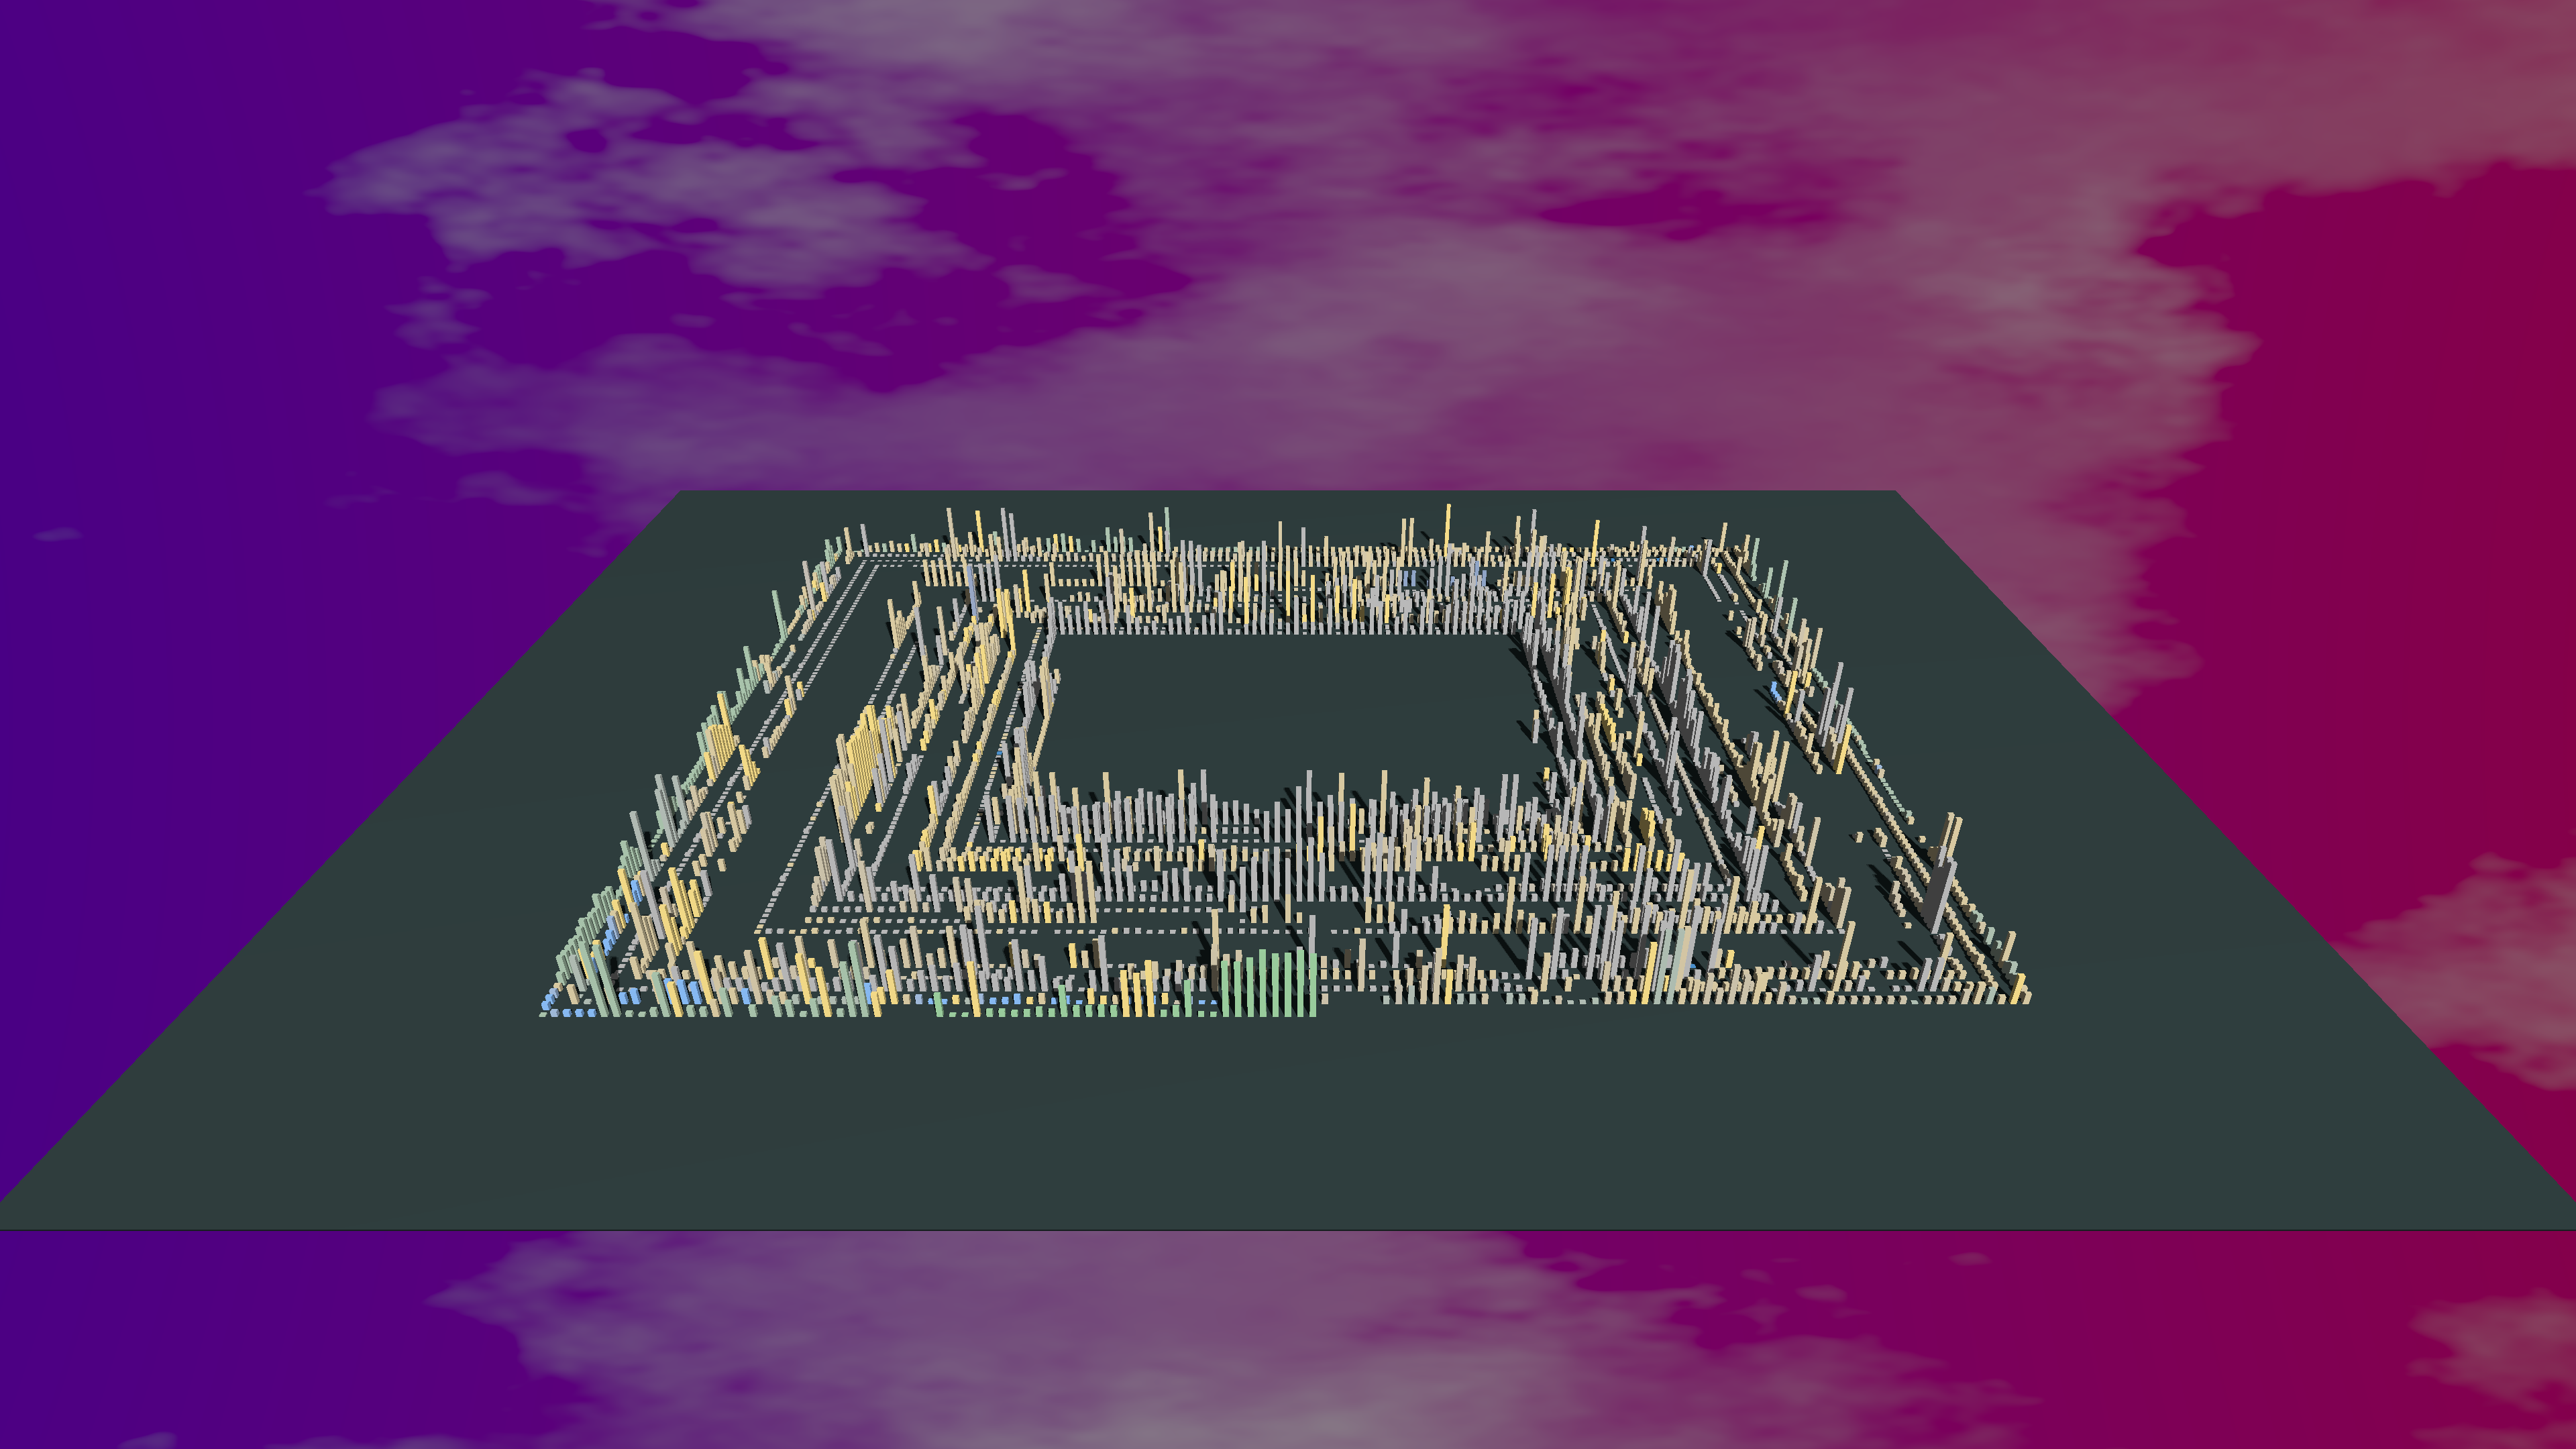
\includegraphics[width=\linewidth]{ArgoUML/Animation006.png}
        \caption{ArgoUML in January 2006 (6 years)} 
        \label{fig:ArgoUML_V3_S3}
    \end{subfigure}\hspace*{\fill}
    \begin{subfigure}{0.48\textwidth}
        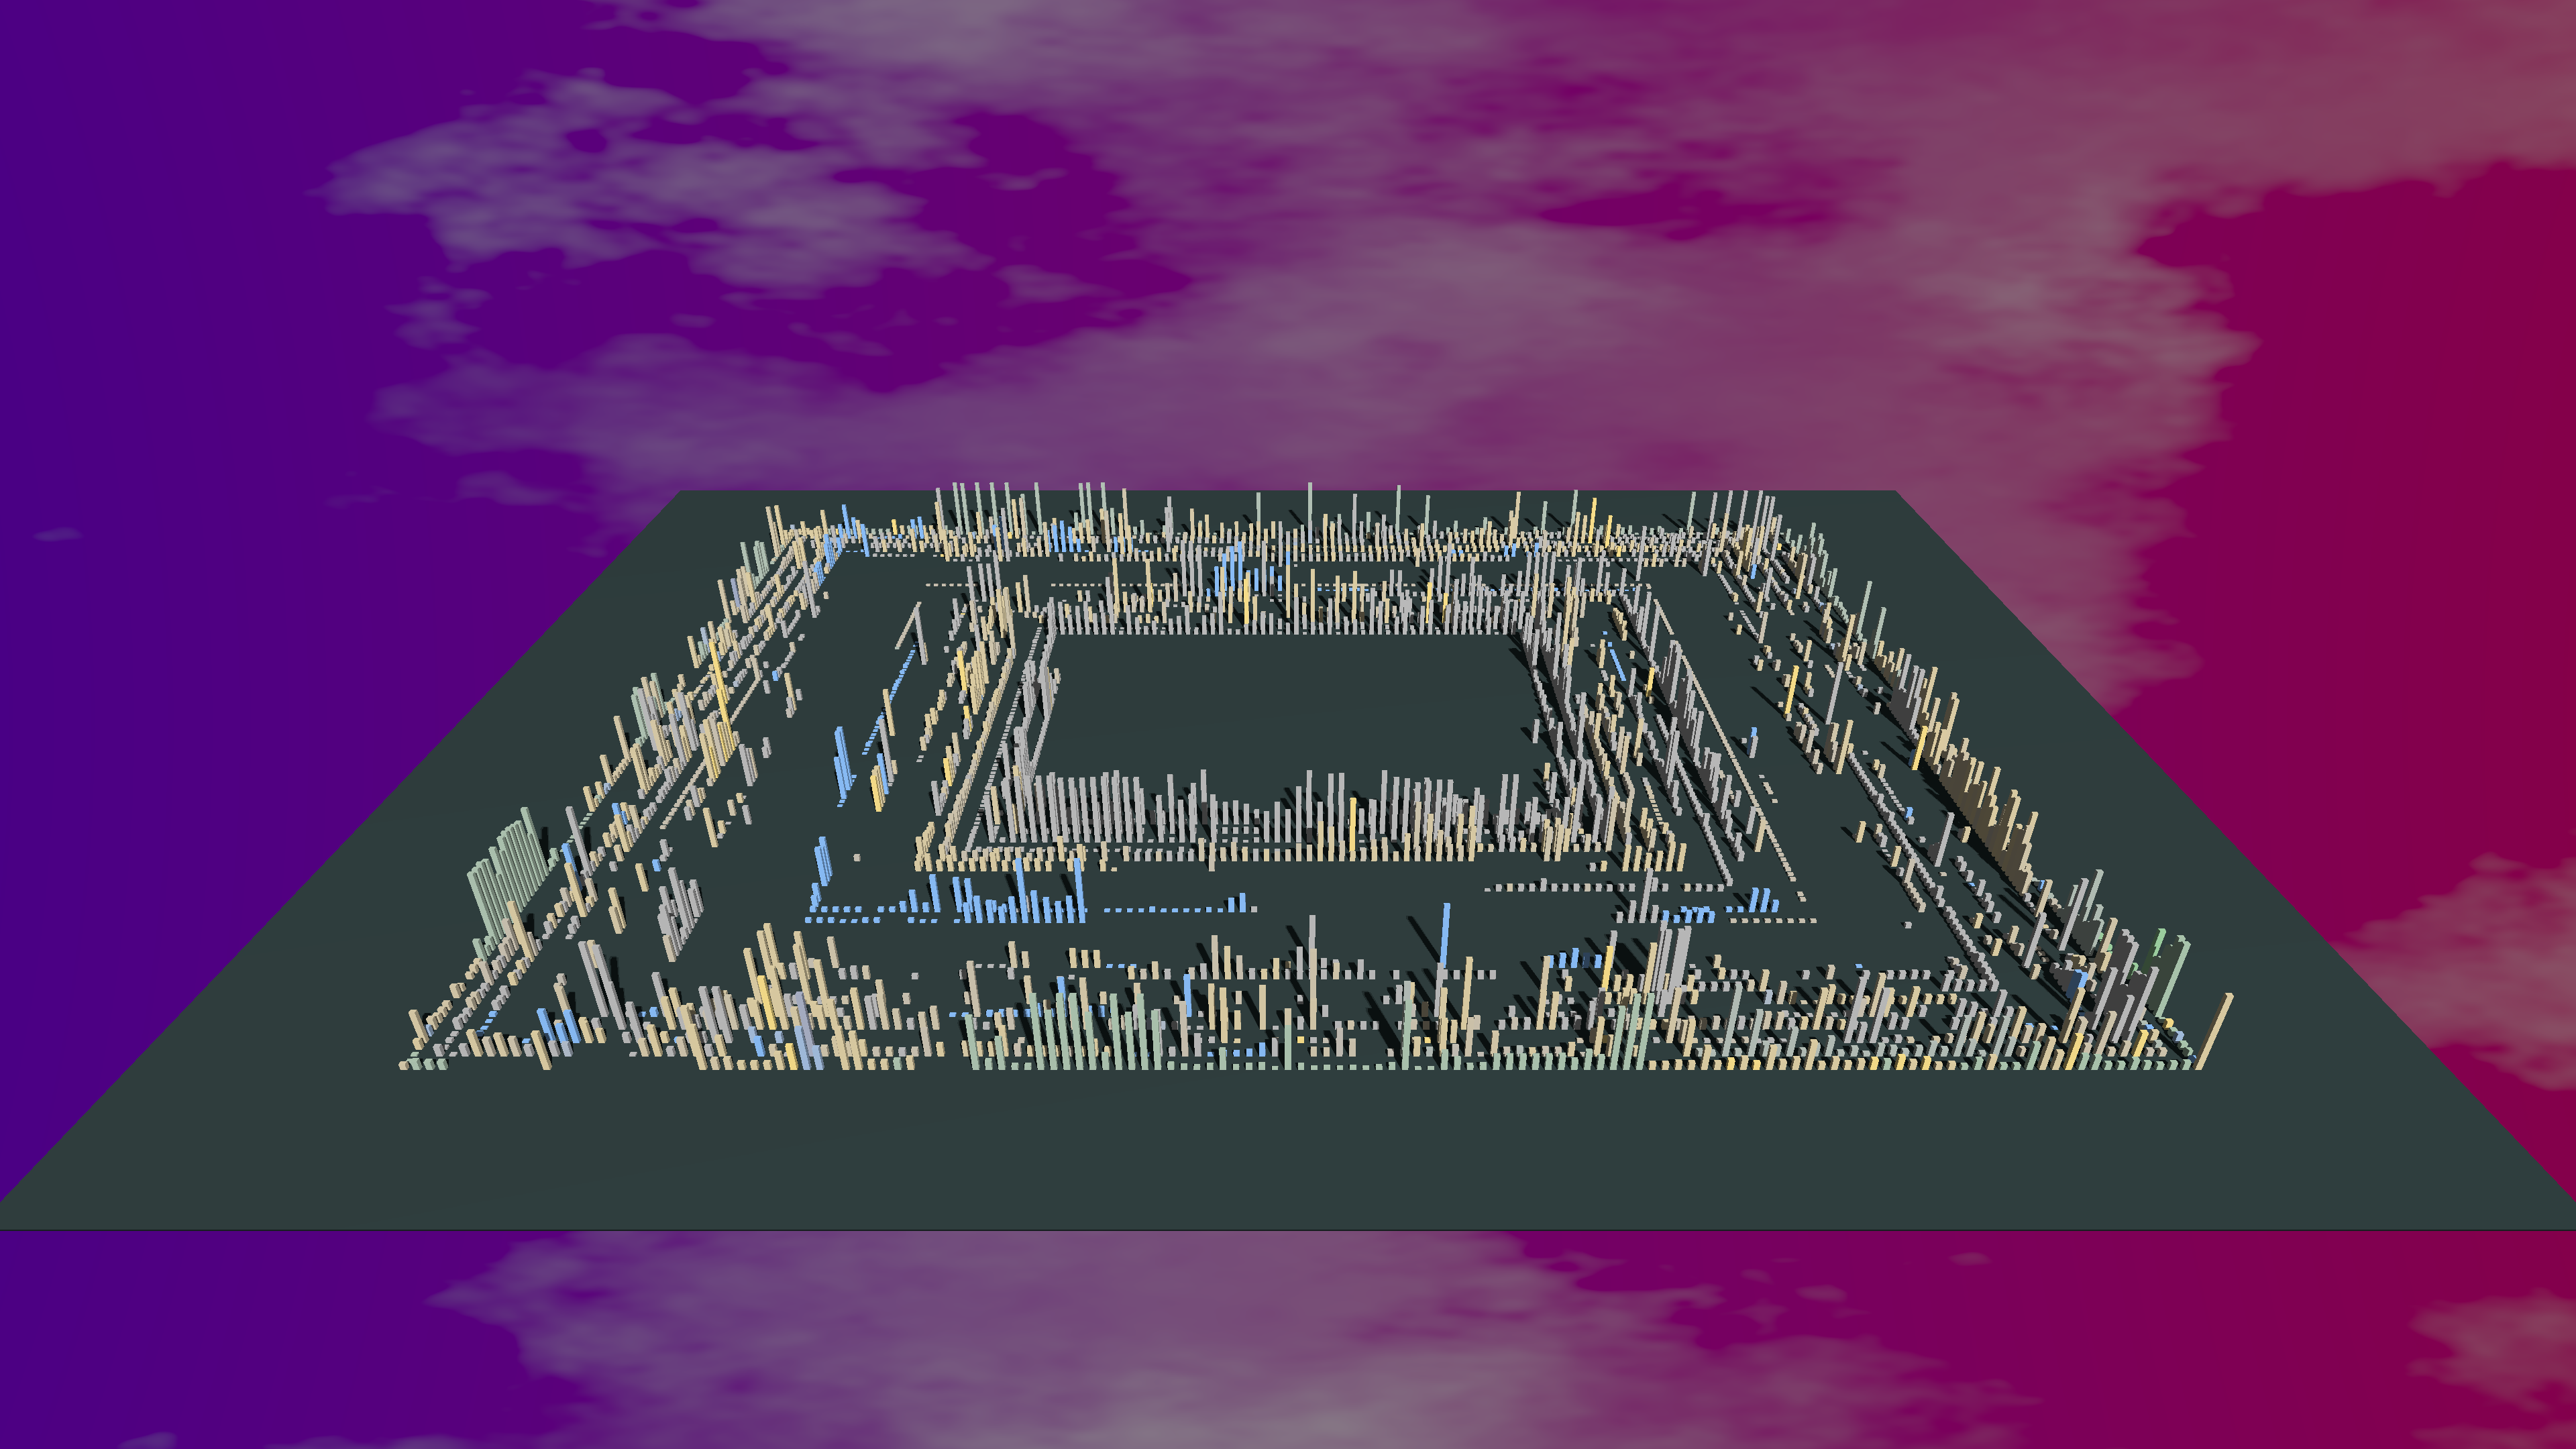
\includegraphics[width=\linewidth]{ArgoUML/Animation010.png}
        \caption{ArgoUML in January 2008 (10 years)} 
        \label{fig:ArgoUML_V3_S4}
    \end{subfigure}
    \medskip
    \begin{subfigure}{0.48\textwidth}
        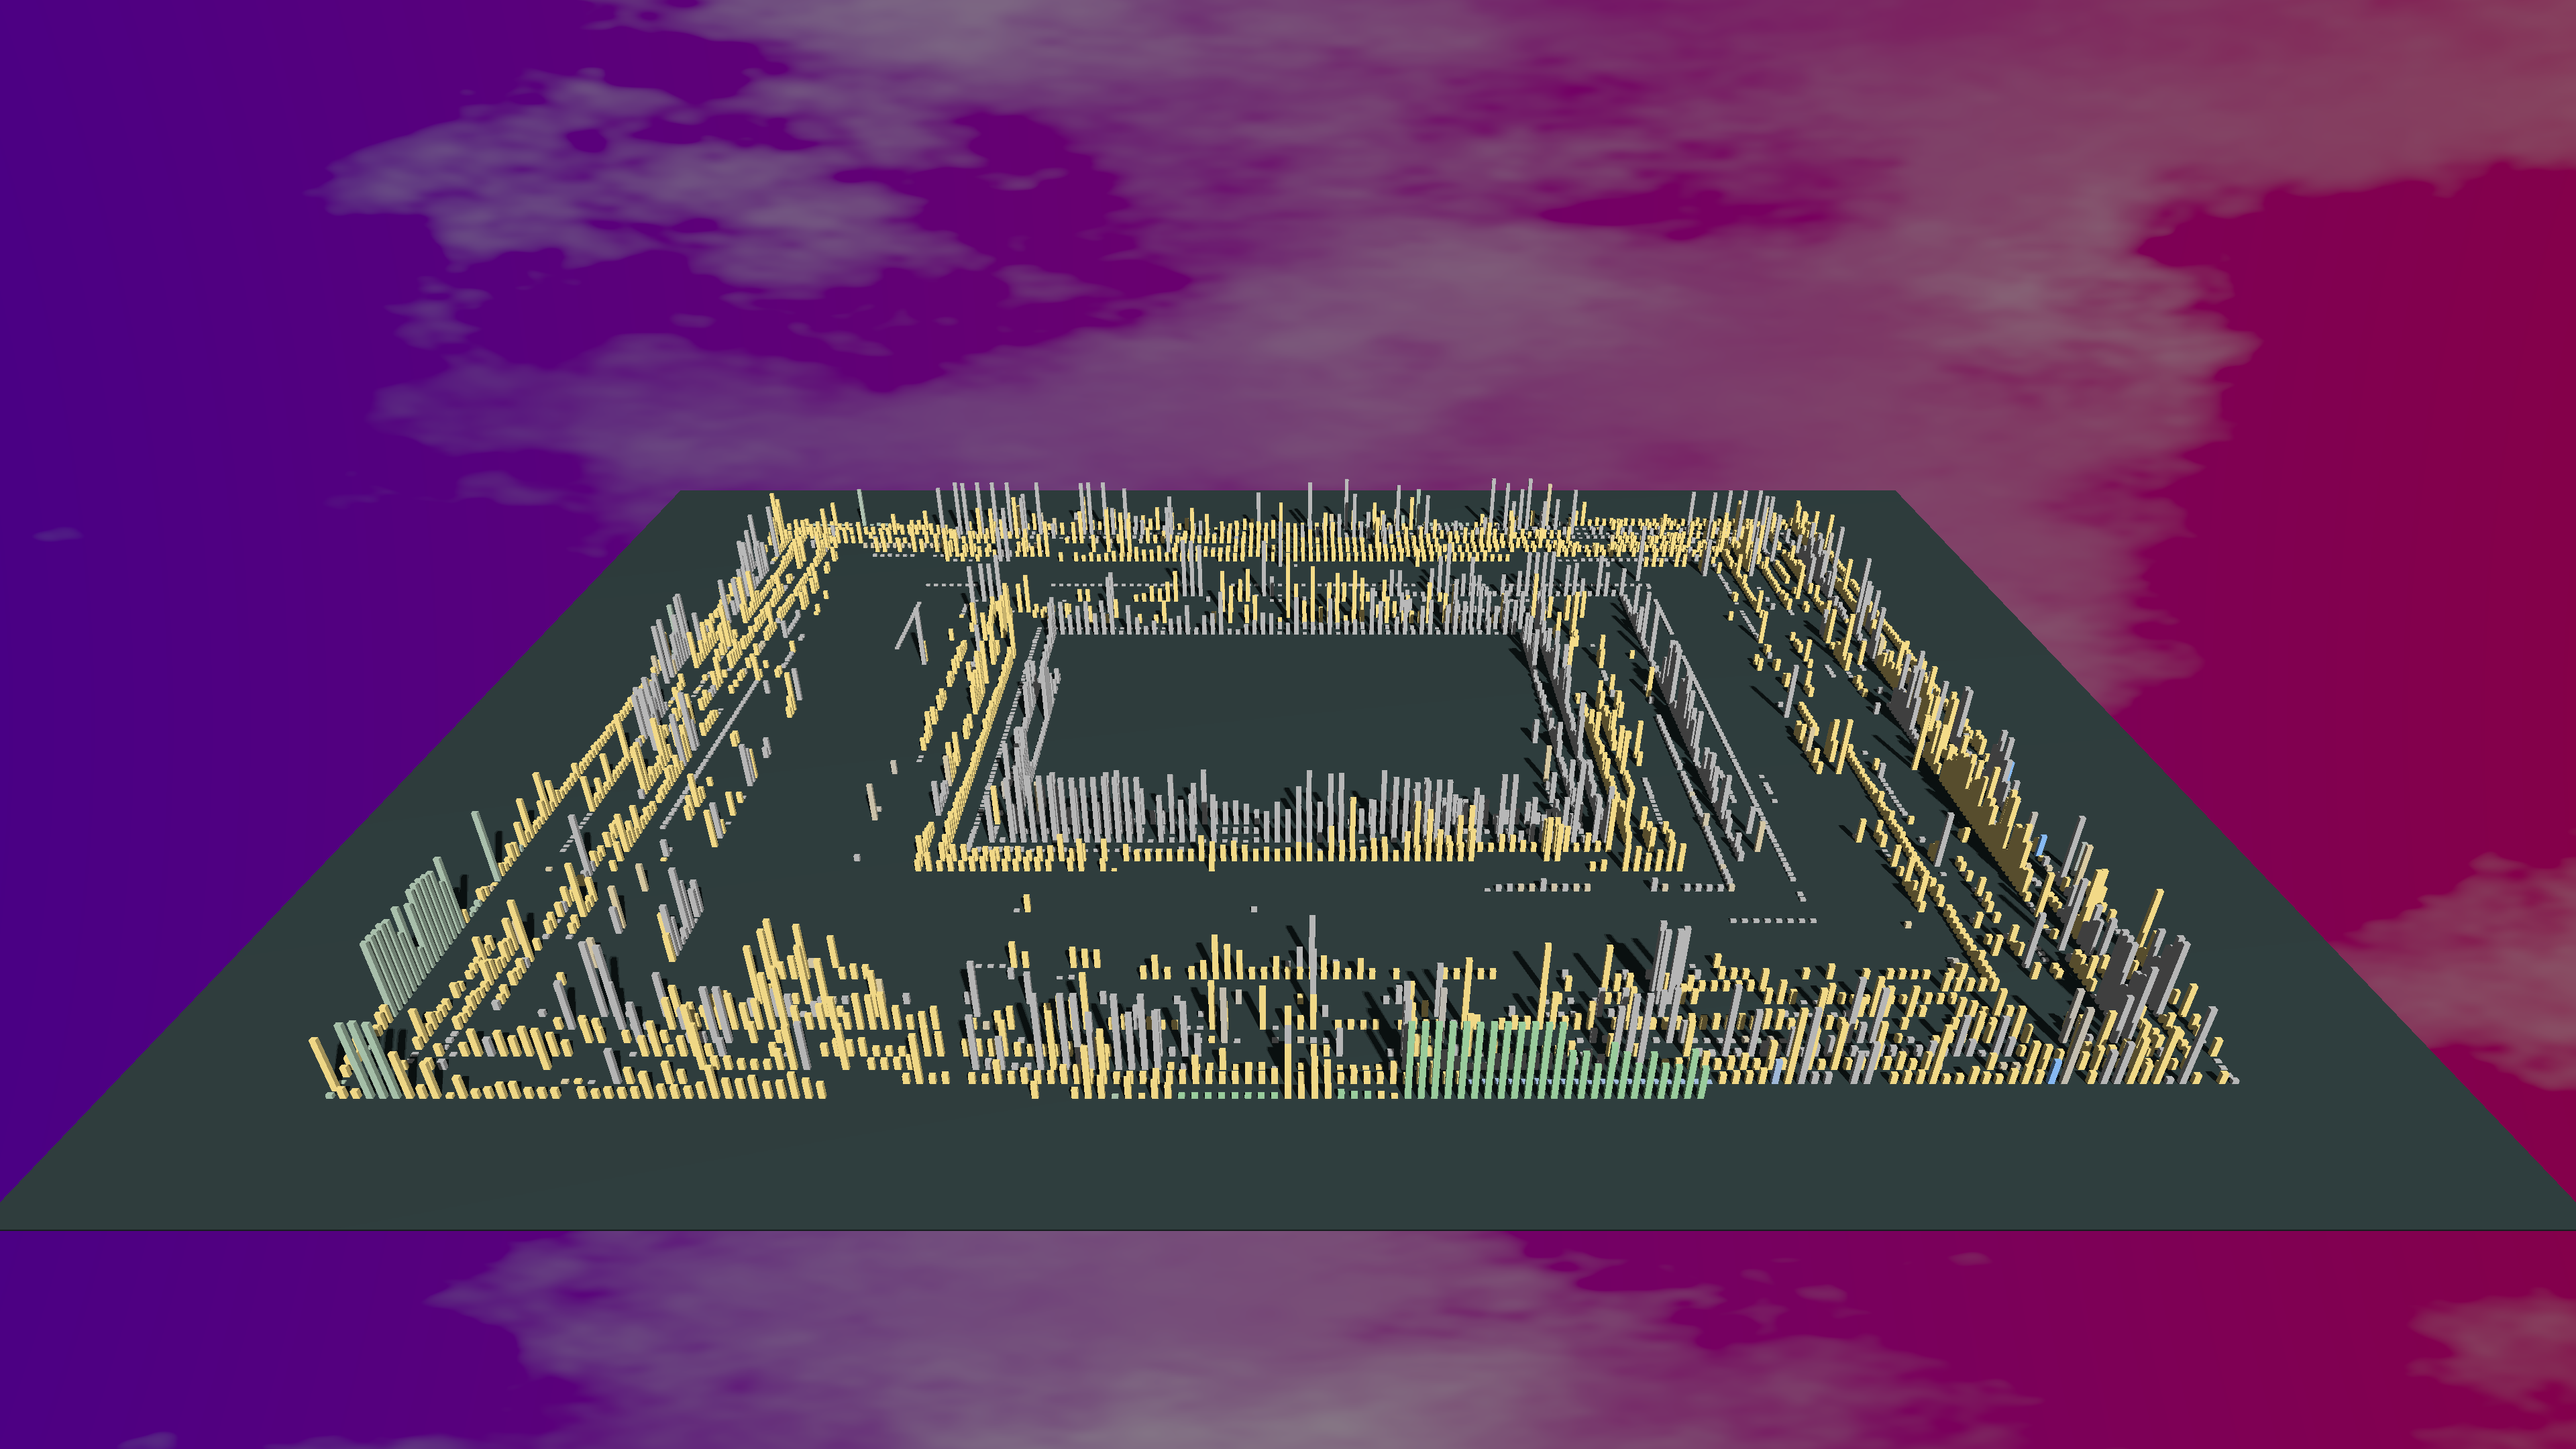
\includegraphics[width=\linewidth]{ArgoUML/Animation012.png}
        \caption{ArgoUML in January 2010 (12 years)} 
        \label{fig:ArgoUML_V3_S5}
    \end{subfigure}\hspace*{\fill}
    \begin{subfigure}{0.48\textwidth}
        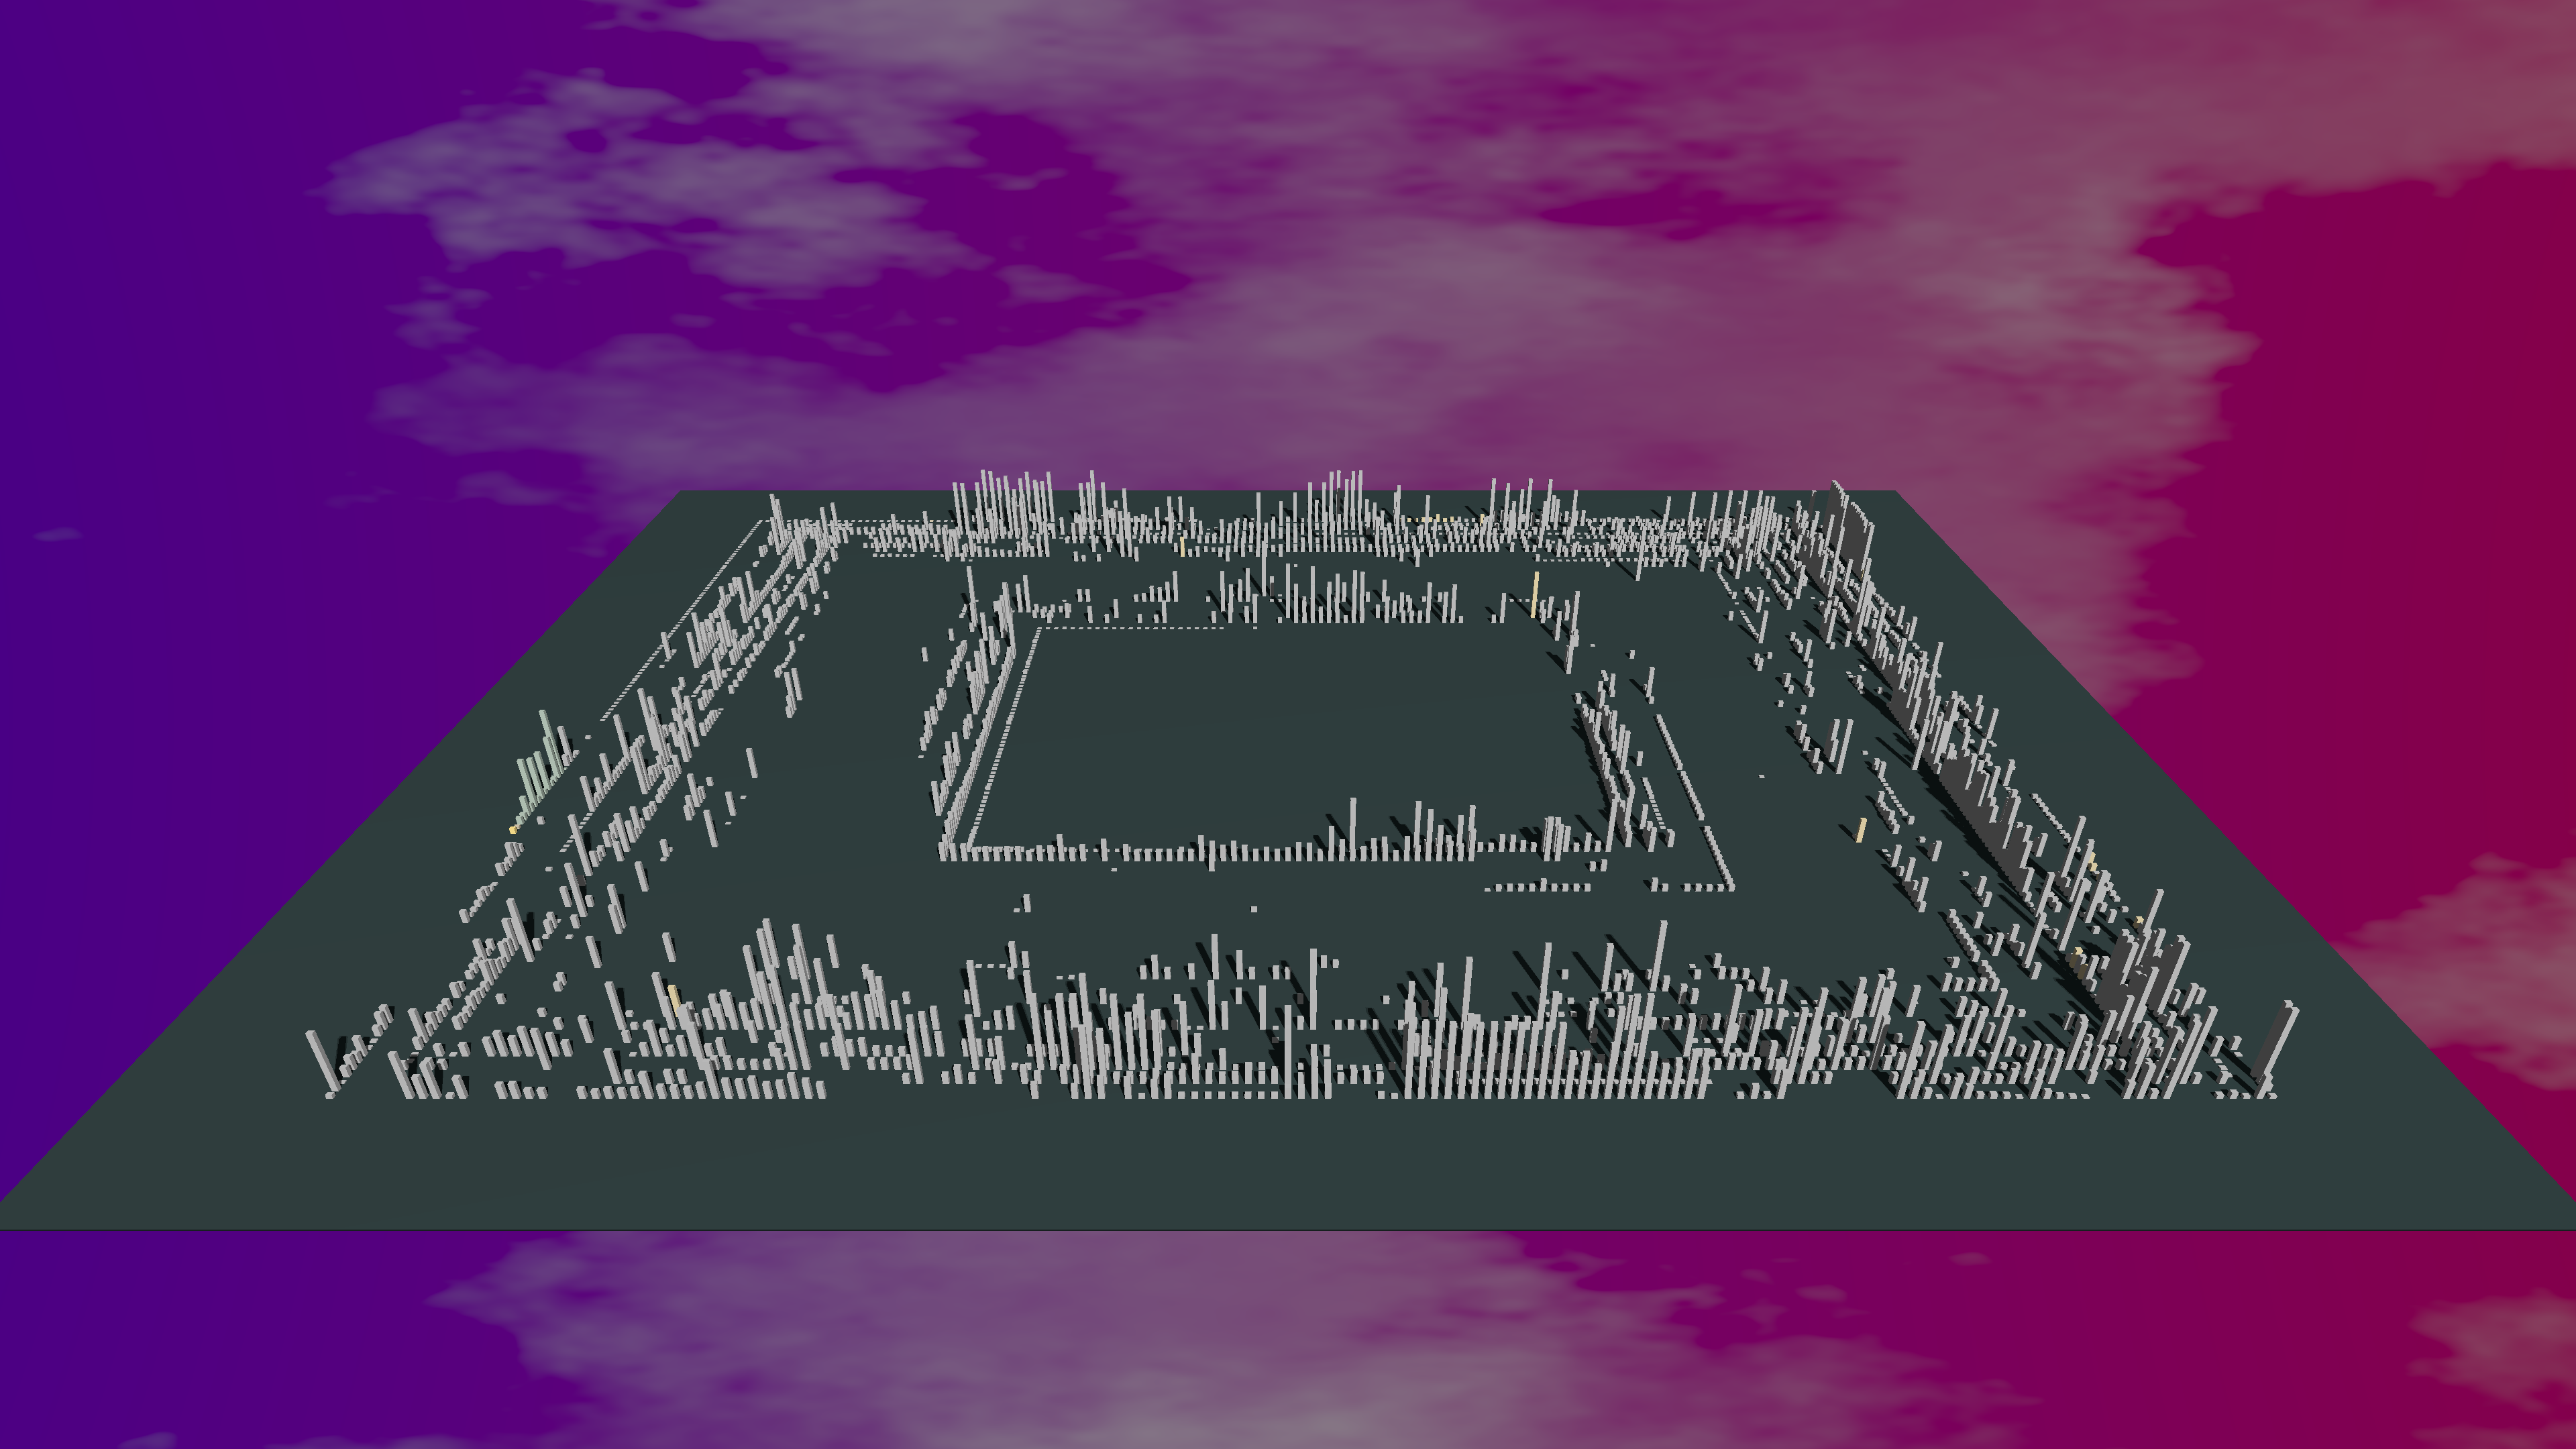
\includegraphics[width=\linewidth]{ArgoUML/Animation022.png}
        \caption{ArgoUML in January 2020 (22 years)} 
        \label{fig:ArgoUML_V3_S6}
    \end{subfigure}
    
    \caption{Hot spots in the evolution of ArgoUML} 
    \label{fig:ArgoUML_V3}
\end{figure}
\clearpage
% -------------------------------------------
% elastic
% FileHistories: 41043 
% ProjectVersions: 34842 
% FileVersions: 326543 
% First Version: 
% 	 hash: 222b36344f0939f12cf54358e7047239cd398463 
% 	 date: Fri Jun 28 09:22:10 CEST 2013 
% Last Version: 
% 	 hash: 2cdffdce2ab35416bd5b1b7ea889cd0dede5b6c8 
% 	 date: Thu Apr 14 14:36:03 CEST 2022 
% Diff: {DAYS=292, HOURS=5, MINUTES=13, SECONDS=53, MILLISECONDS=0, MICROSECONDS=0, NANOSECONDS=0, YEARS=8}
% -------------------------------------------

\section{Elasticsearch – Forty Thousand File Histories}
This section analyzes Elasticsearch, a distributed, RESTful JSON-based search, and analytics engine. 
The project is open-source and hosted on GitHub.\footnote{\url{https://github.com/elastic/elasticsearch}}
The first commit was made in June 2013, even though it was not the real first one because the project started before being migrated to GitHub, in 2009.
Our analysis includes almost nine years of history, in which there are 34,843 ProjectVersions, 41,043 FileHistories, and more than 300K FileVersions. 

\bigbreak
%\subsection{View 5}
\textbf{Visualization goal:}
This visualization aims to see how the repository evolved through its last nine years. We adopt a commit grouping strategy based on a time window of one year and an aging strategy of one month with 12 steps. Hence, grey entities represent files that have not been updated for more than 12 months. 


View specification adopted: 
\begin{itemize}
    \item \texttt{versionGroupingStrategy}: timestamp.
    \item \texttt{versionGroupingChunkSize}: 31,556,926 (1 year). 
    \item \texttt{colorPalette}: default.
    \item \texttt{agingGroupingStrategy}: timestamp.
    \item \texttt{agingStepSize}: 2,629,743 (1 month).
    \item \texttt{agingSteps}: 12 steps.
    \item \texttt{mapperMetricName}: SIZE. 
    \item \texttt{fileTypeShape}: all BOX. 
    \item \texttt{fileTypeOpacity}: all 1. 
\end{itemize}
\bigbreak
\textbf{Results:}
Here we present only the relevant aspects of ArgoUML's evolution that we have found and present its full story in \autoref{app:Elastic_Evolution}. \autoref{fig:Elastic_V5} shows the hot spots during the system's evolution. \autoref{fig:Elastic_V5_S1} shows the initial size of the system when the system became open source and was officially moved on GitHub. After one year of inactivity, the size of the system in June 2016 was almost triple of two years before. In June 2014, it had 2,904 files; in June 2016, it had 9,537 files. However, in \autoref{fig:Elastic_V5_S2}, we notice that only the entities around the center of the system were touched. This means that the initial implementation of Elasticsearch remained untouched and that not many of the files added in 2013 were modified. Perhaps the code was stable enough that it did not require much maintenance, and only new features were added before June 2016. After a one-year break, in June 2018, they had another big increment in the system, as shown in \autoref{fig:Elastic_V5_S3}. It doubled its size again. Interestingly, the core remained untouched, except for very few changes. Moreover, the height of entities present in \autoref{fig:Elastic_V5_S2} became higher. This not only means that they were modified, but it might also mean that new features were added to these classes. We recorded the same growth pattern later until June 2022. As depicted in \autoref{fig:Elastic_V5_S4}, \autoref{fig:Elastic_V5_S5}, \autoref{fig:Elastic_V5_S6} the system incremented the number and size of files gradually. The most important thing is that, except for the center, most of the files are painted with a bright color, meaning they are maintained. 


\bigbreak
\textbf{Conclusion:} This analysis highlighted interesting aspects of Elasticsearch's evolution. The core of the system, once developed, was never touched, except for very few entities. As we can notice in  \autoref{fig:Elastic_V5}, the core is always depicted in gray, even when files around it are modified in the last year of evolution. 

\begin{figure}[ht]
    \begin{subfigure}{0.48\textwidth}
        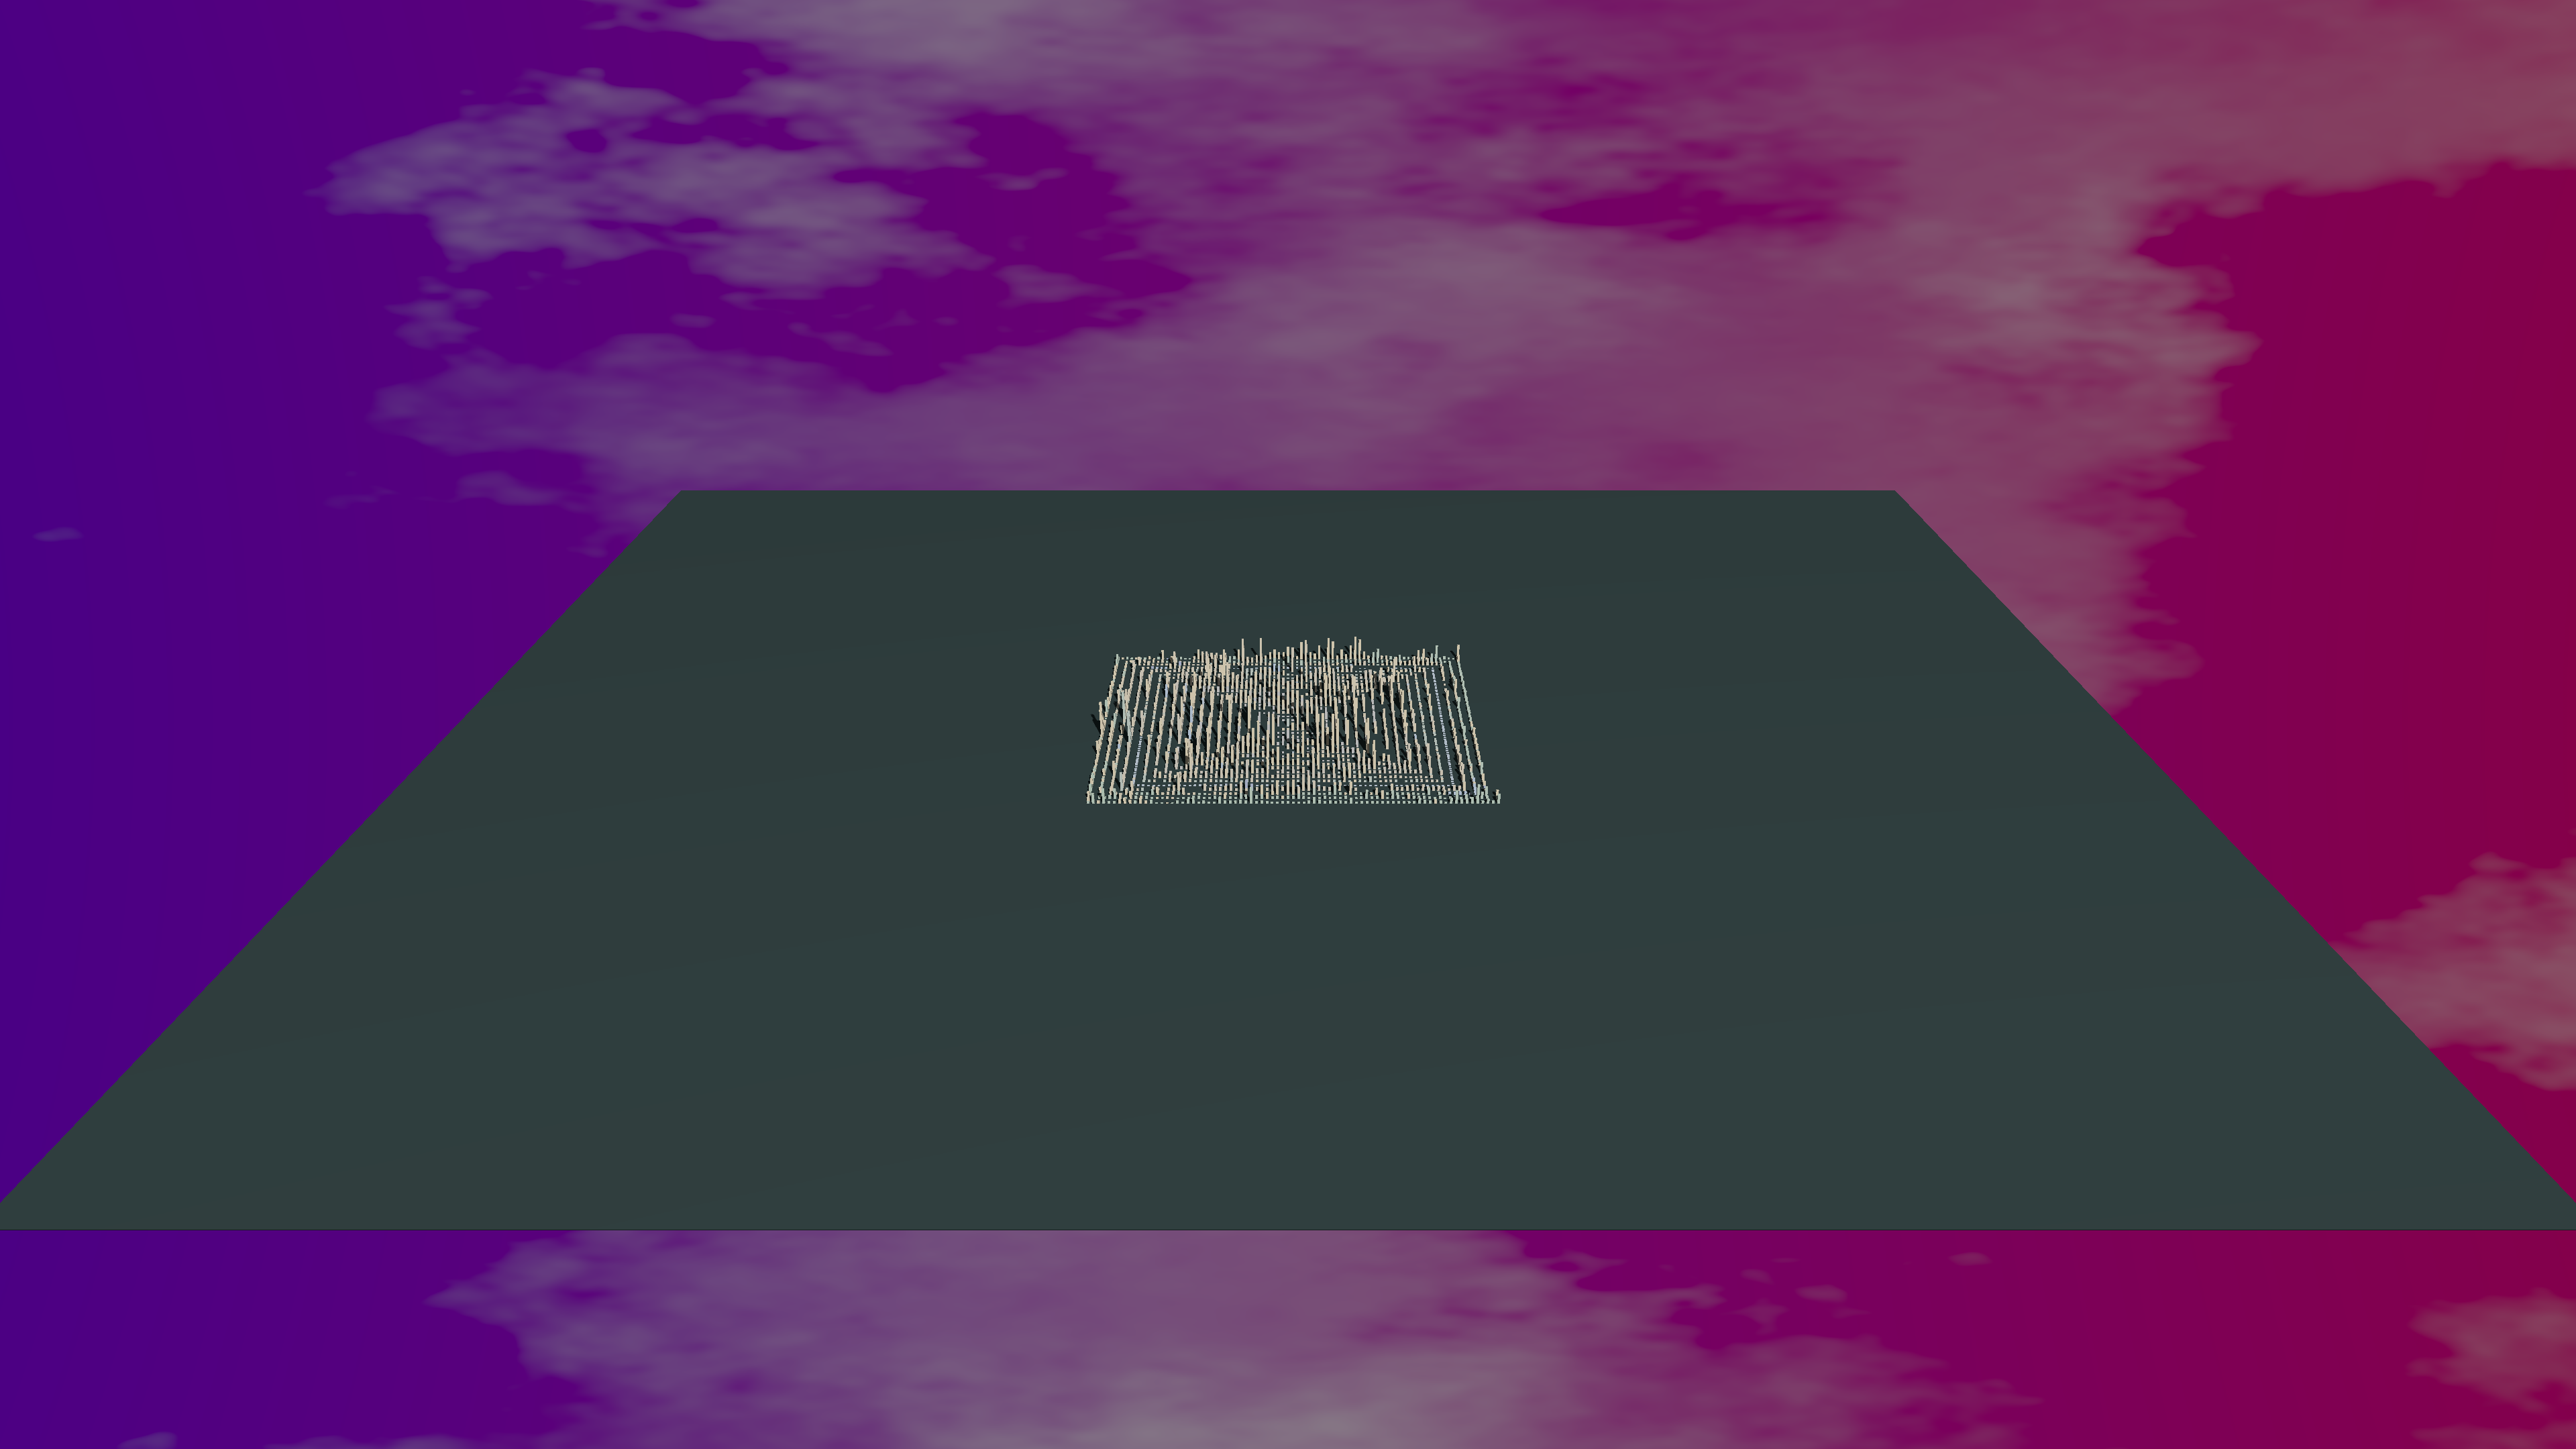
\includegraphics[width=\linewidth]{Elasticsearch/Animation001.png}
        \caption{Elasticsearch in June 2014 (1 year)} 
        \label{fig:Elastic_V5_S1}
    \end{subfigure}\hspace*{\fill}
    \begin{subfigure}{0.48\textwidth}
        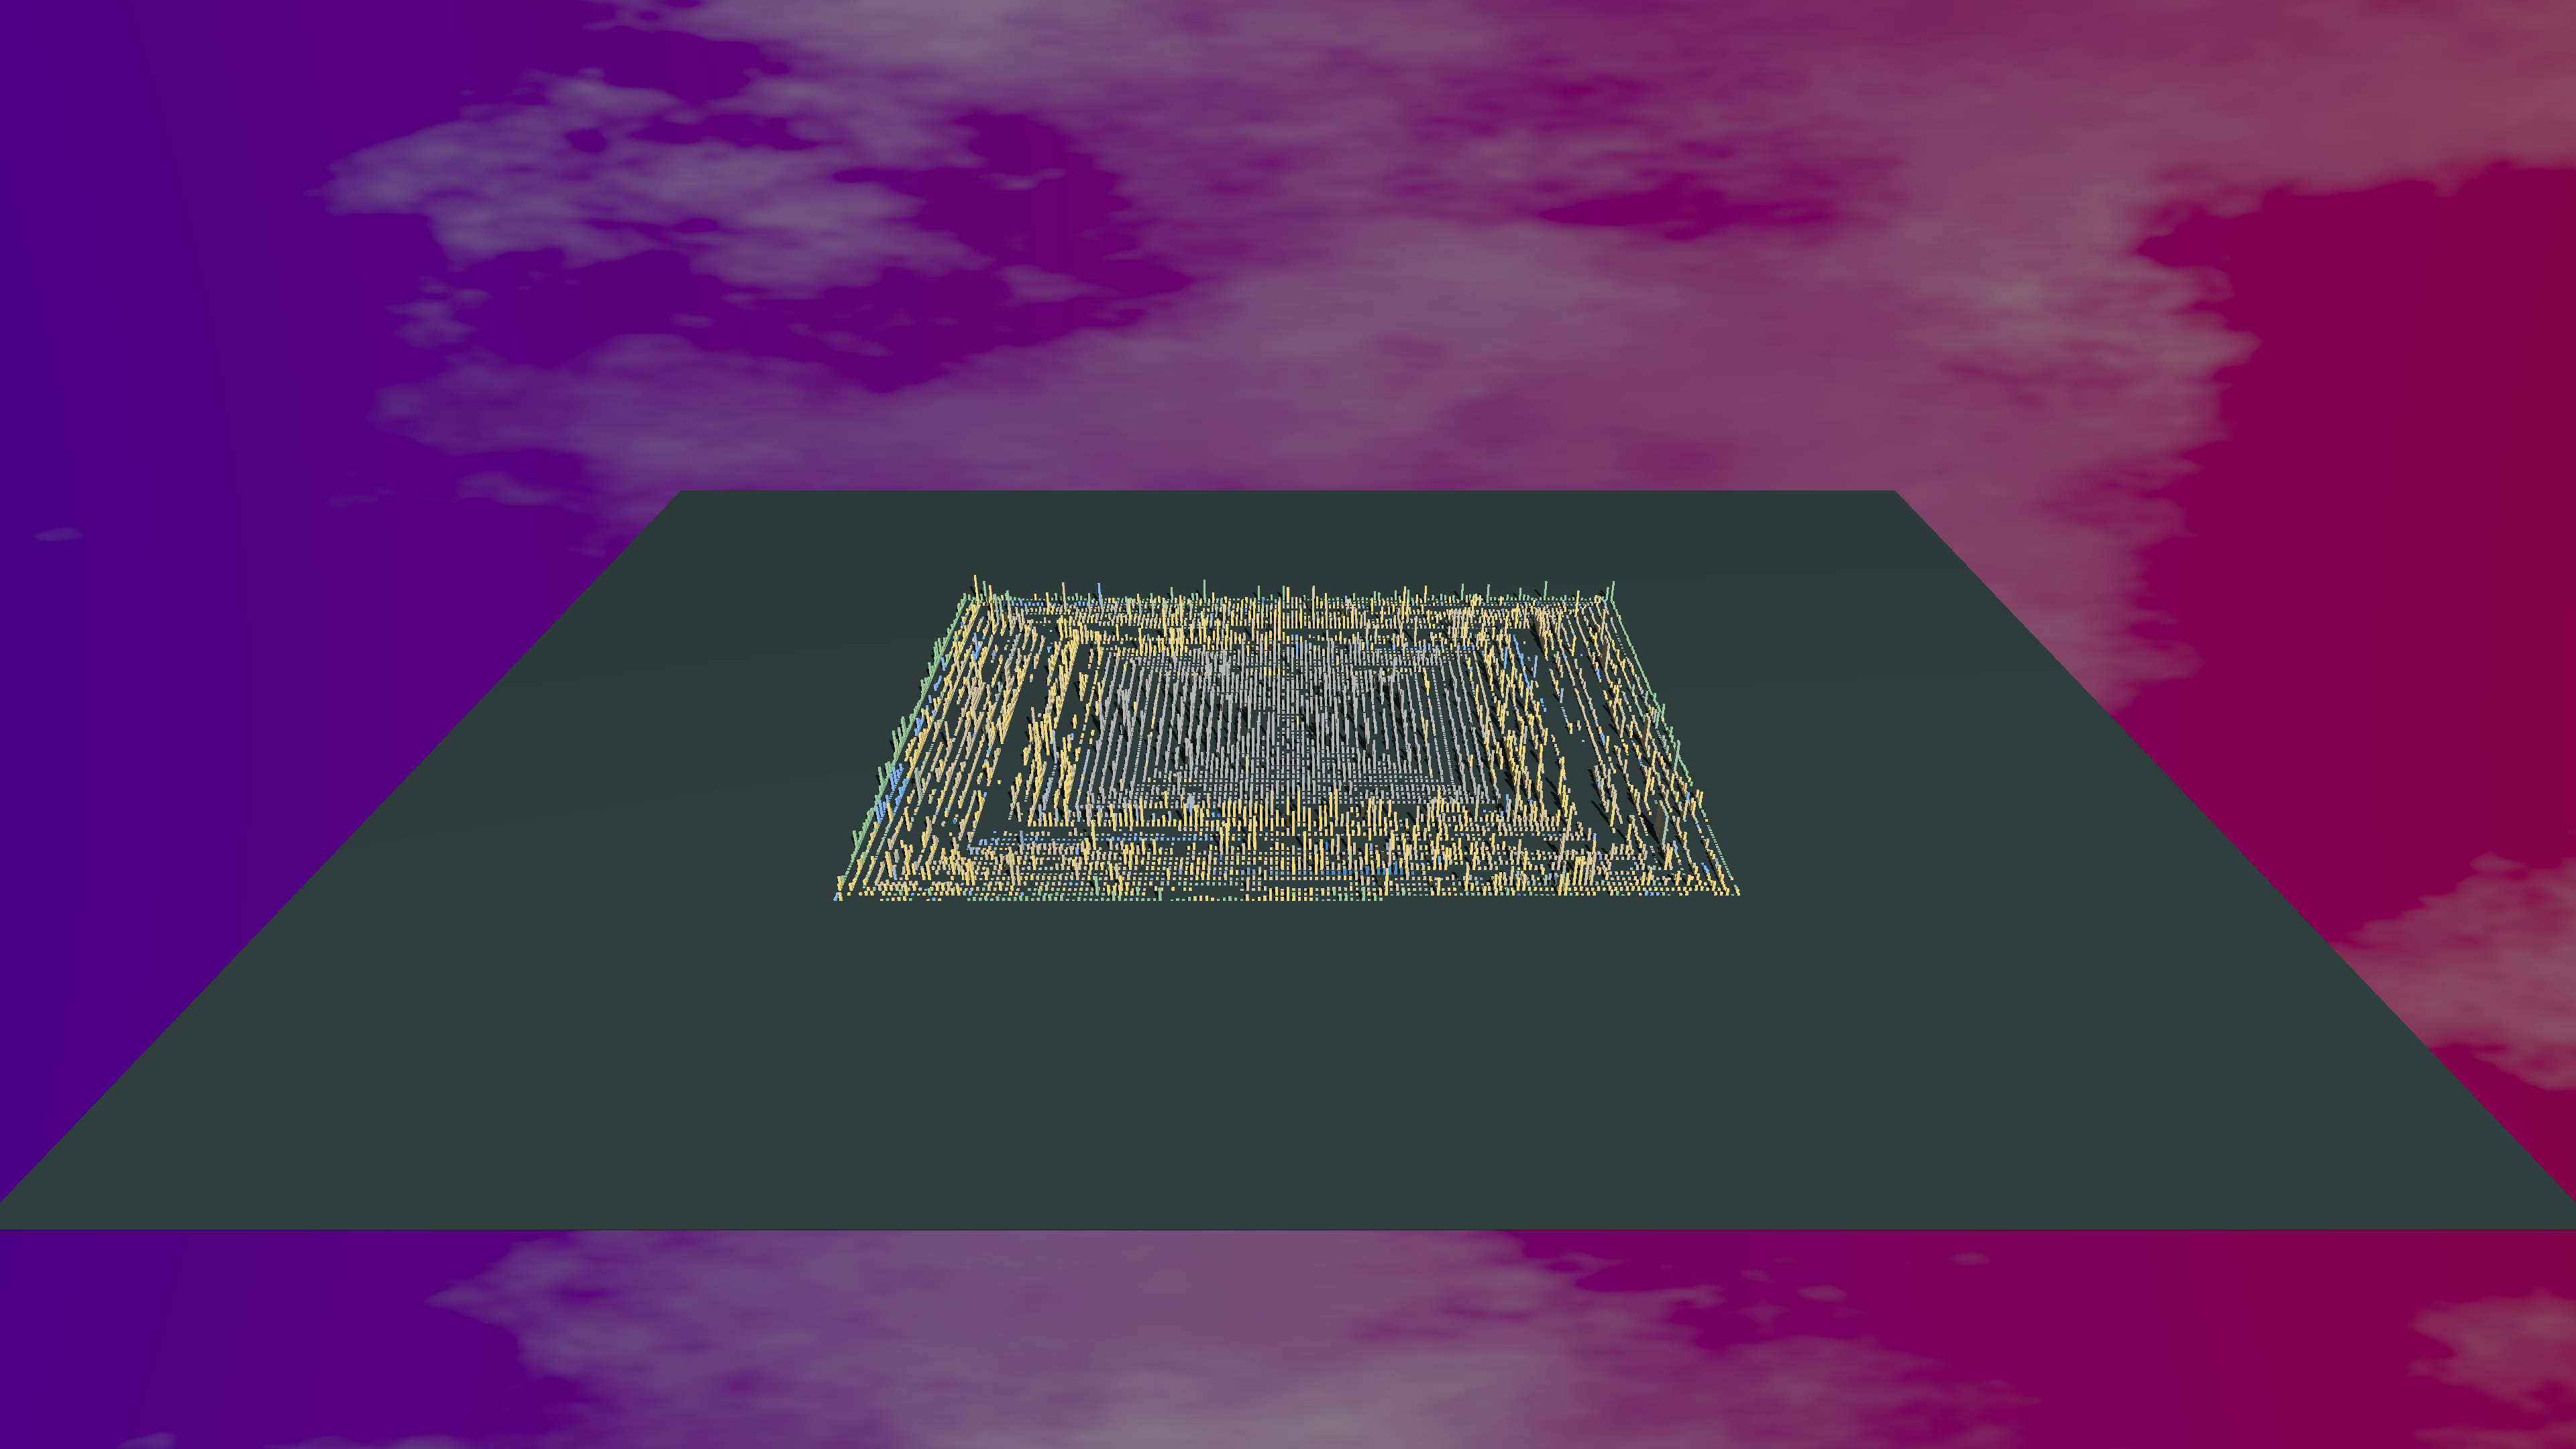
\includegraphics[width=\linewidth]{Elasticsearch/Animation003.png}
        \caption{Elasticsearch in June 2016 (3 year)} 
        \label{fig:Elastic_V5_S2}
    \end{subfigure}
    \medskip
    \begin{subfigure}{0.48\textwidth}
        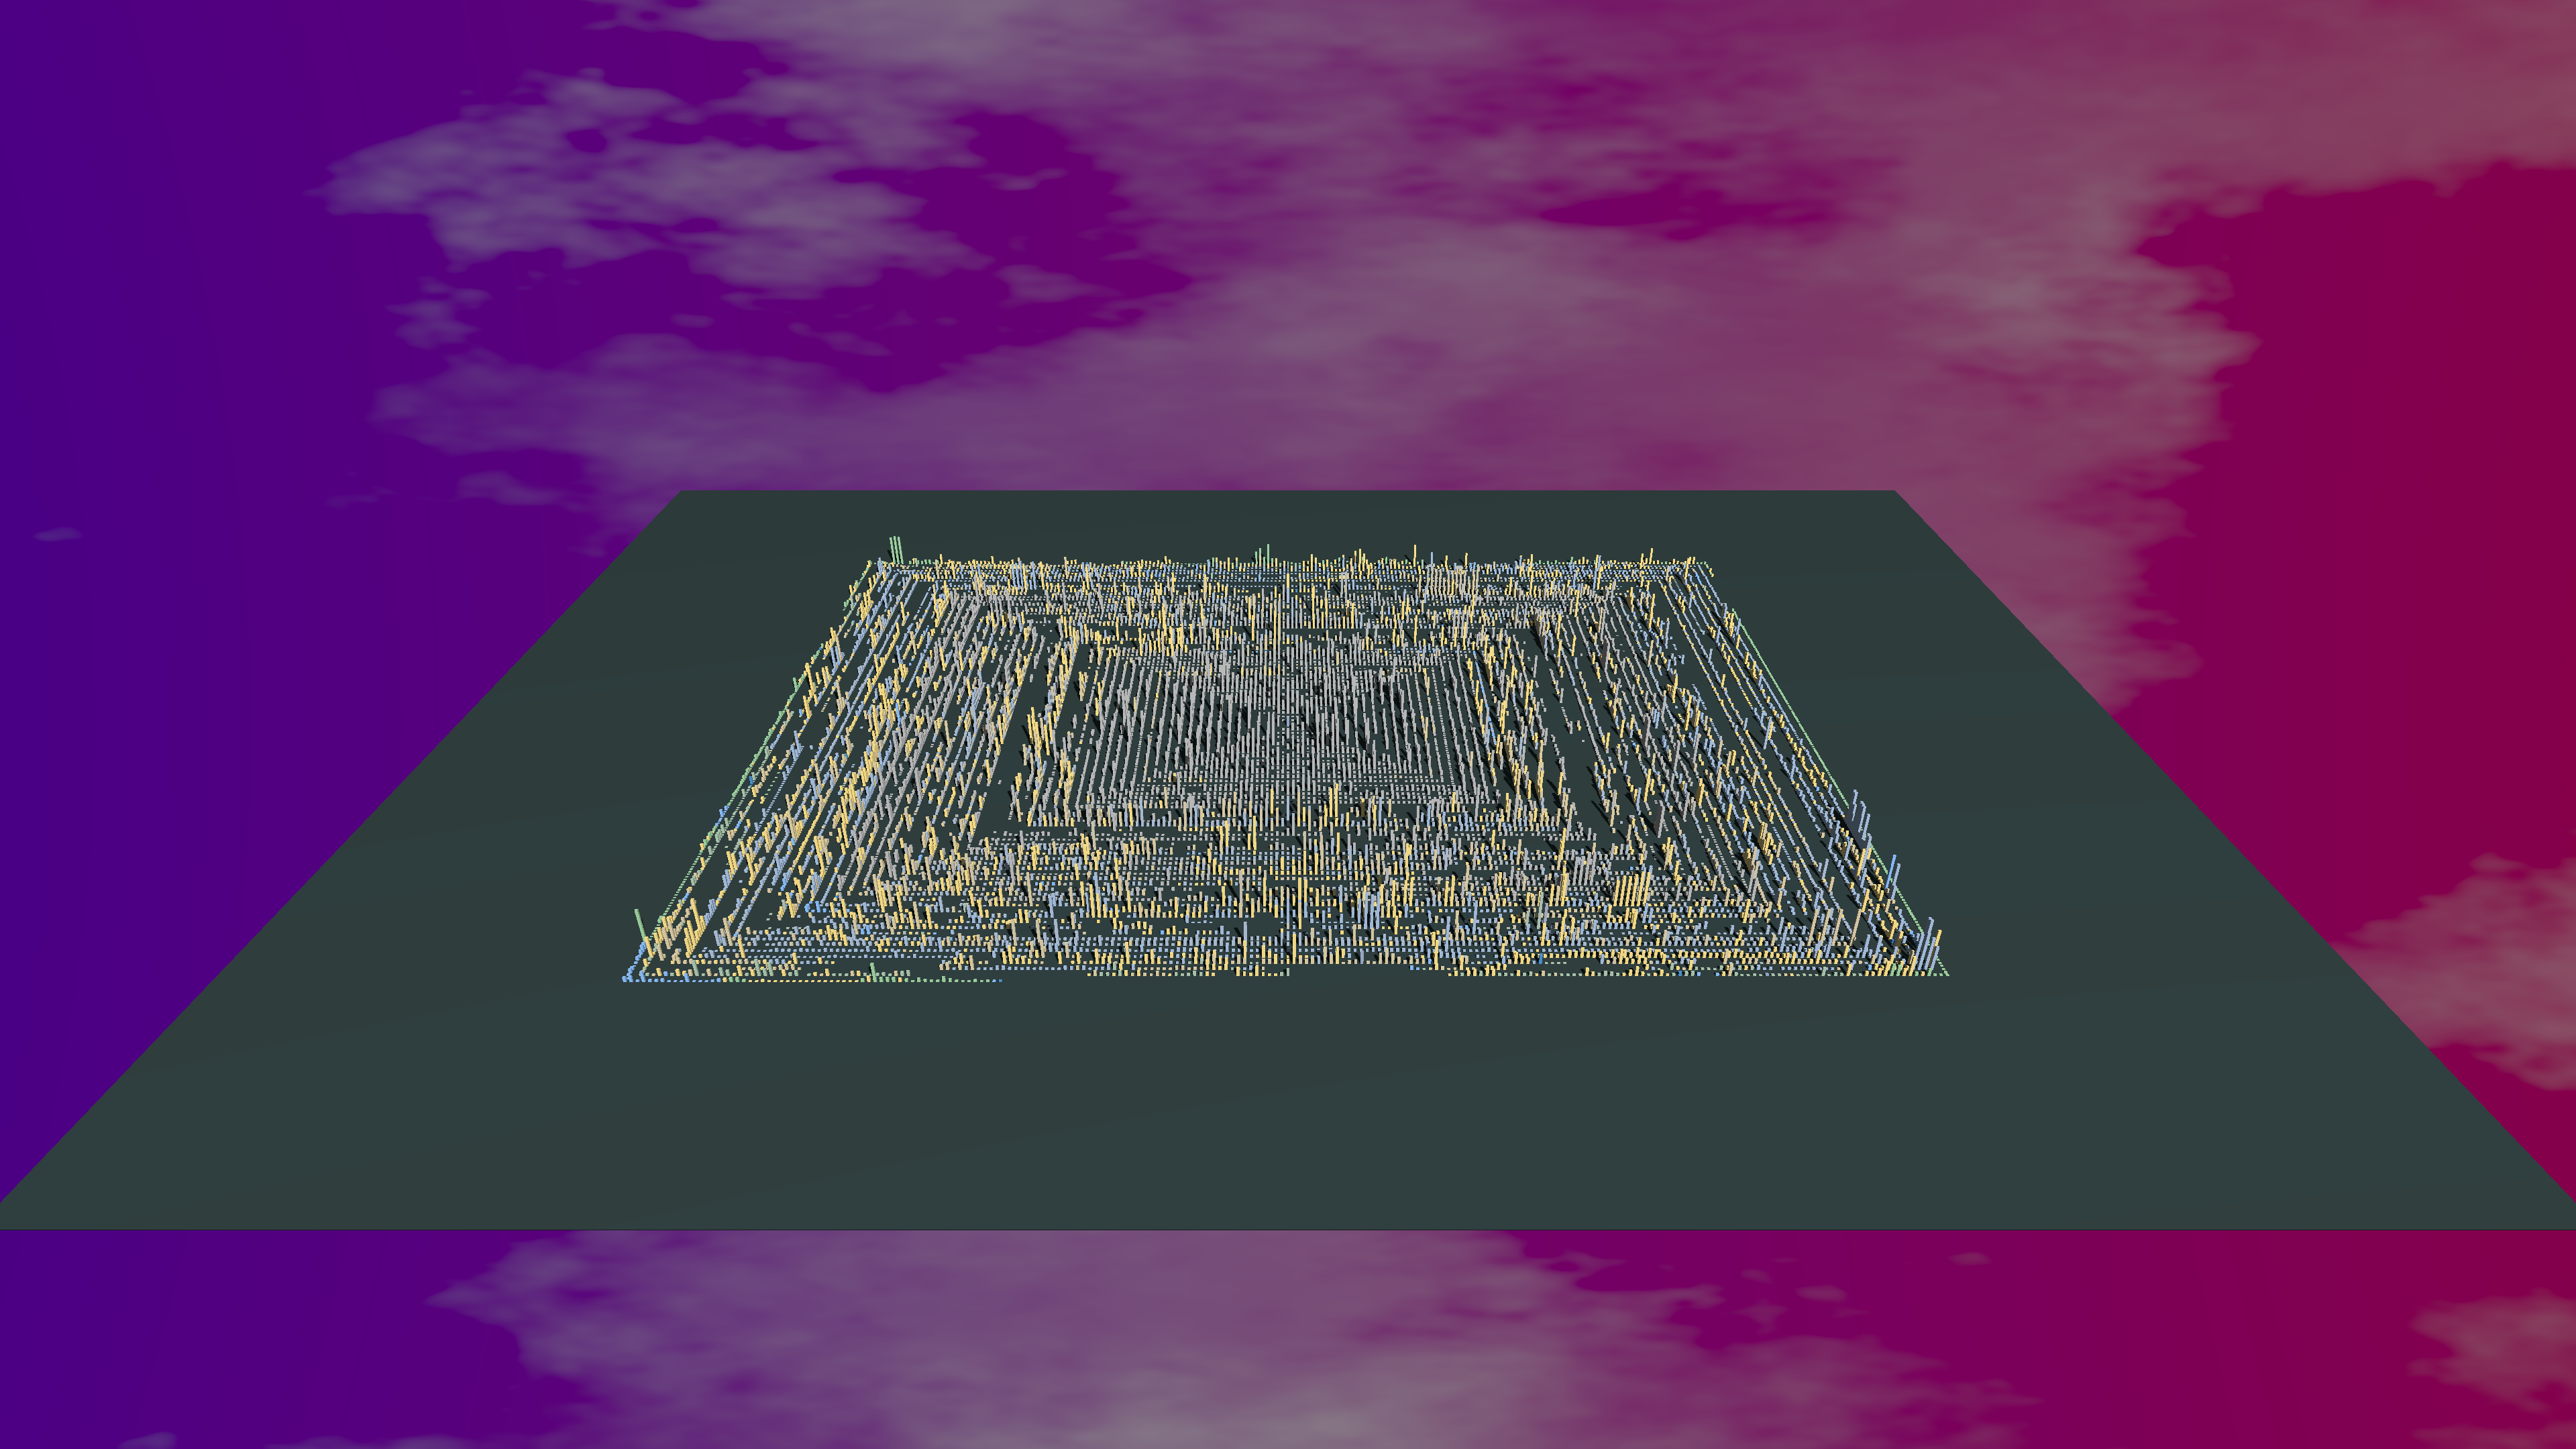
\includegraphics[width=\linewidth]{Elasticsearch/Animation005.png}
        \caption{Elasticsearch in June 2018 (5 year)} 
        \label{fig:Elastic_V5_S3}
    \end{subfigure}\hspace*{\fill}
    \begin{subfigure}{0.48\textwidth}
        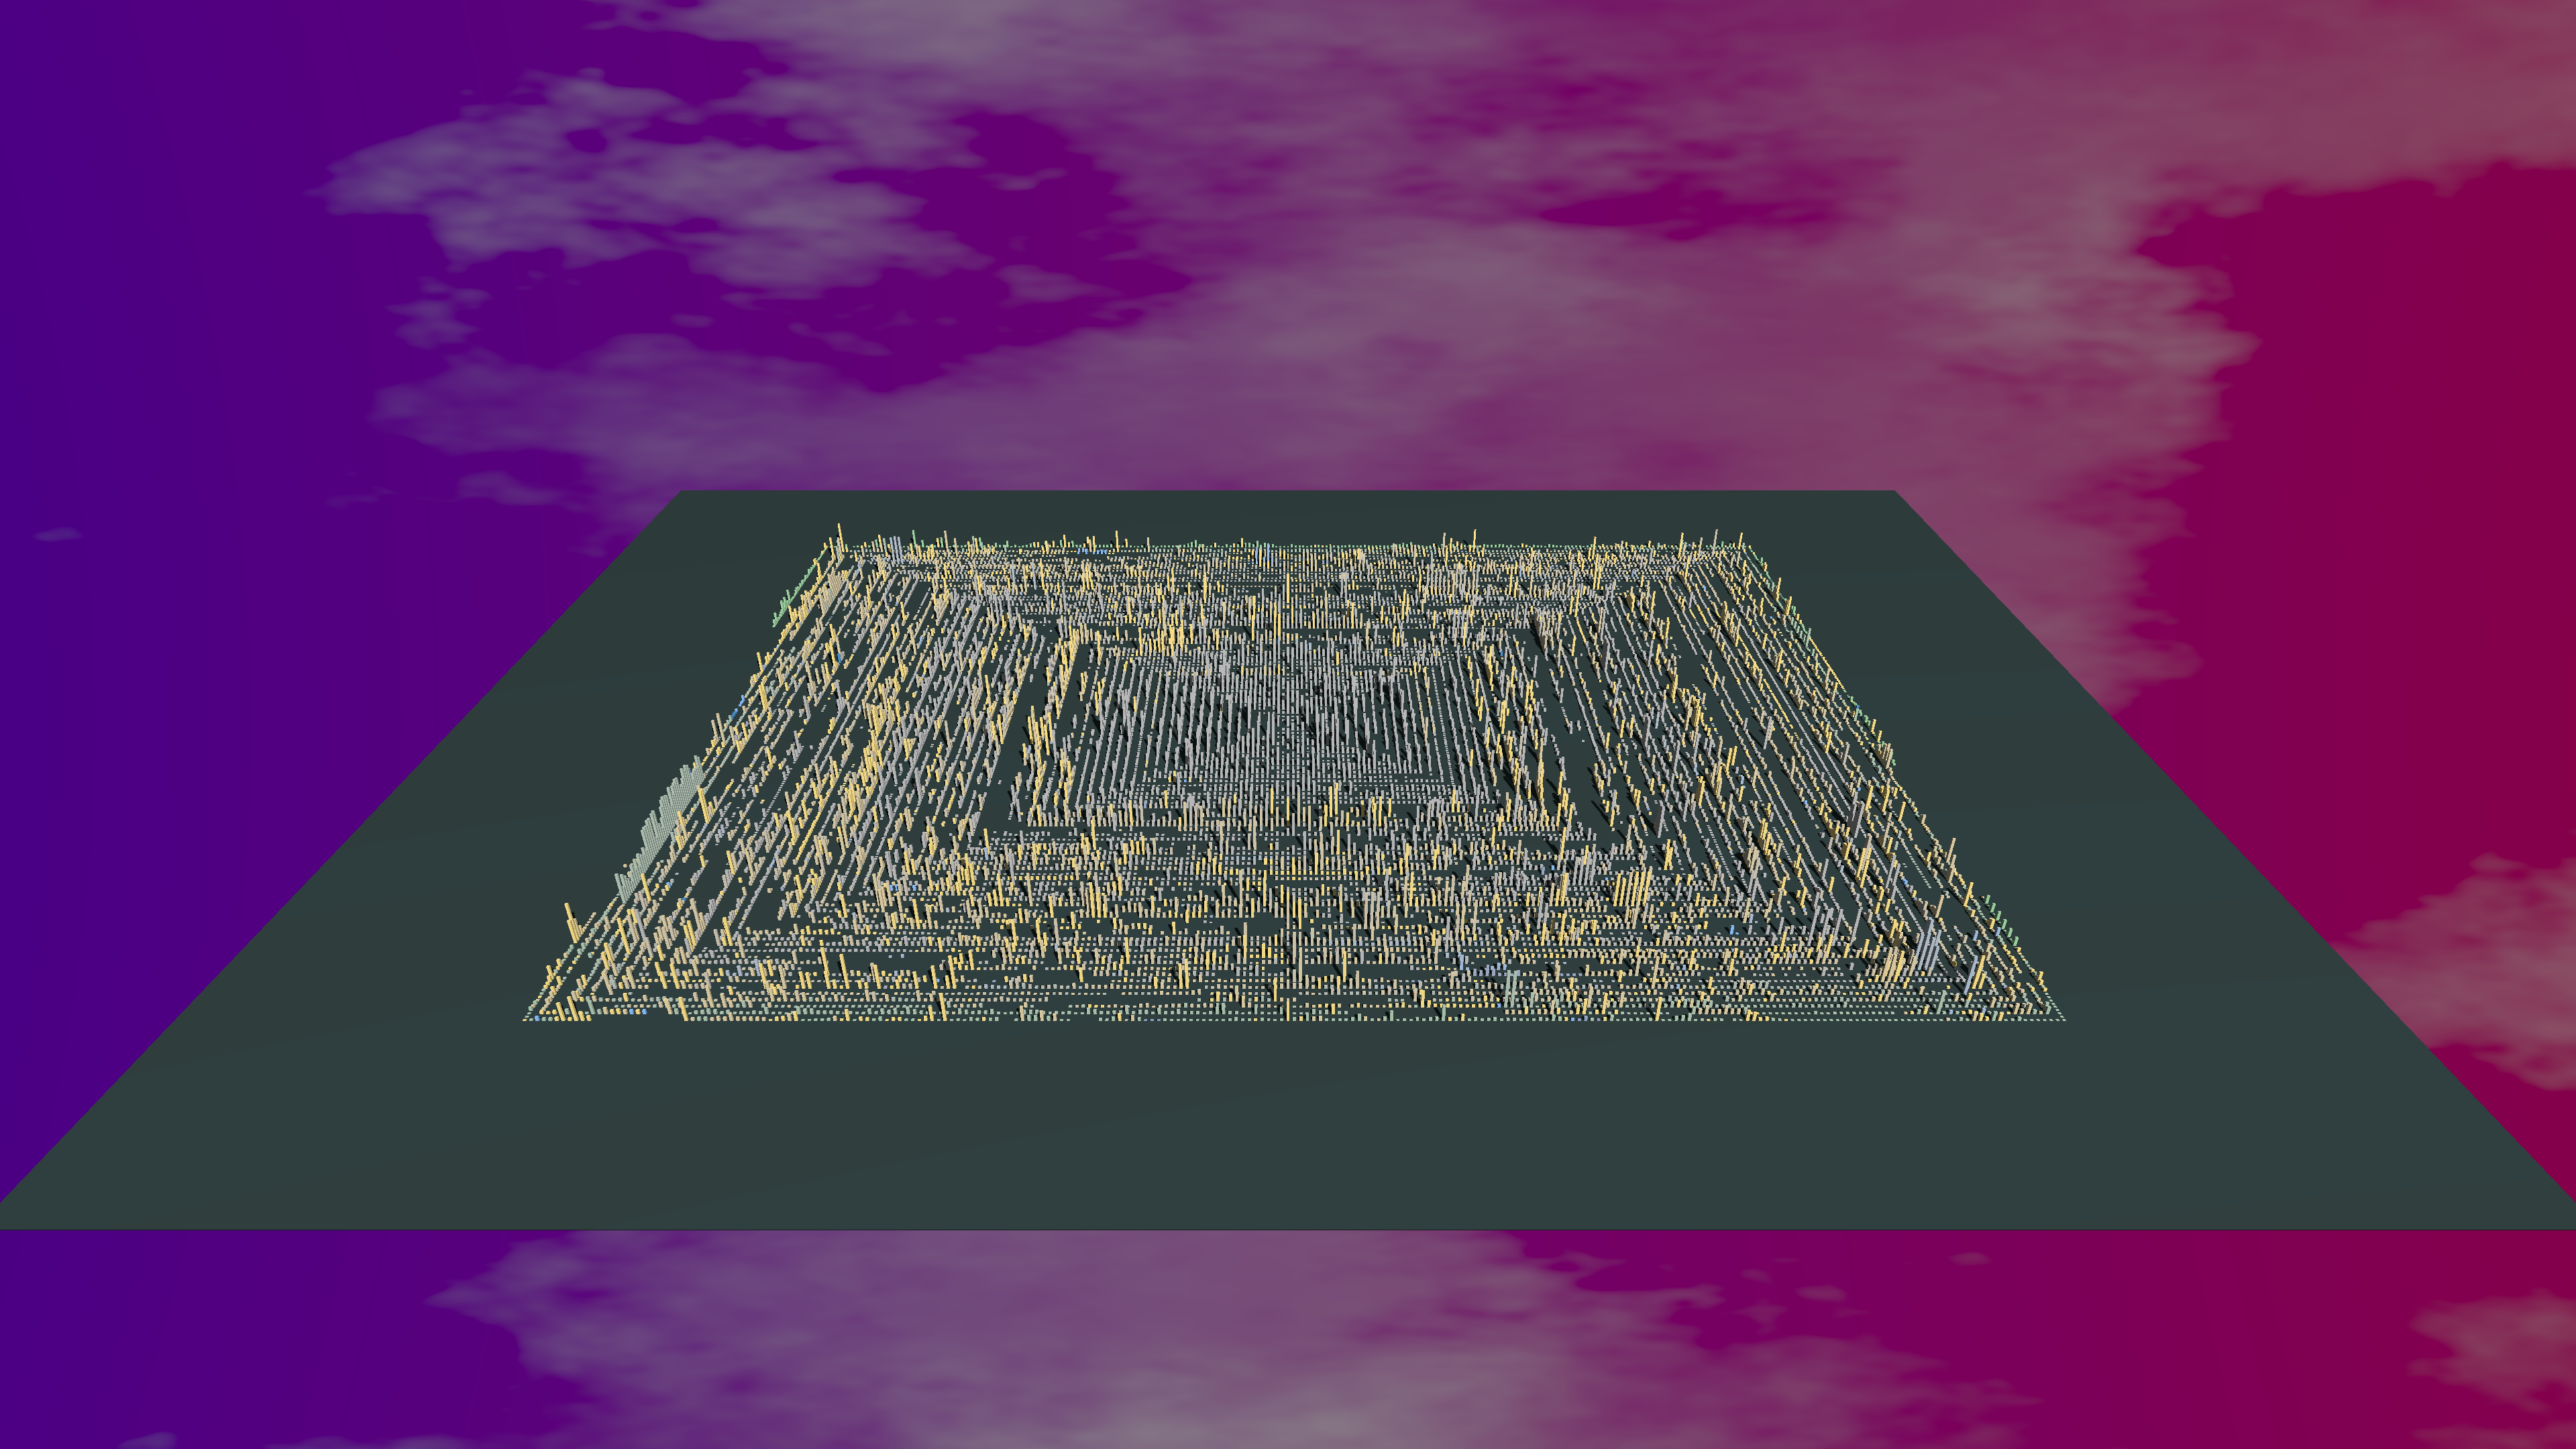
\includegraphics[width=\linewidth]{Elasticsearch/Animation006.png}
        \caption{Elasticsearch in June 2019  (6 year)} 
        \label{fig:Elastic_V5_S4}
    \end{subfigure}
    \medskip
    \begin{subfigure}{0.48\textwidth}
        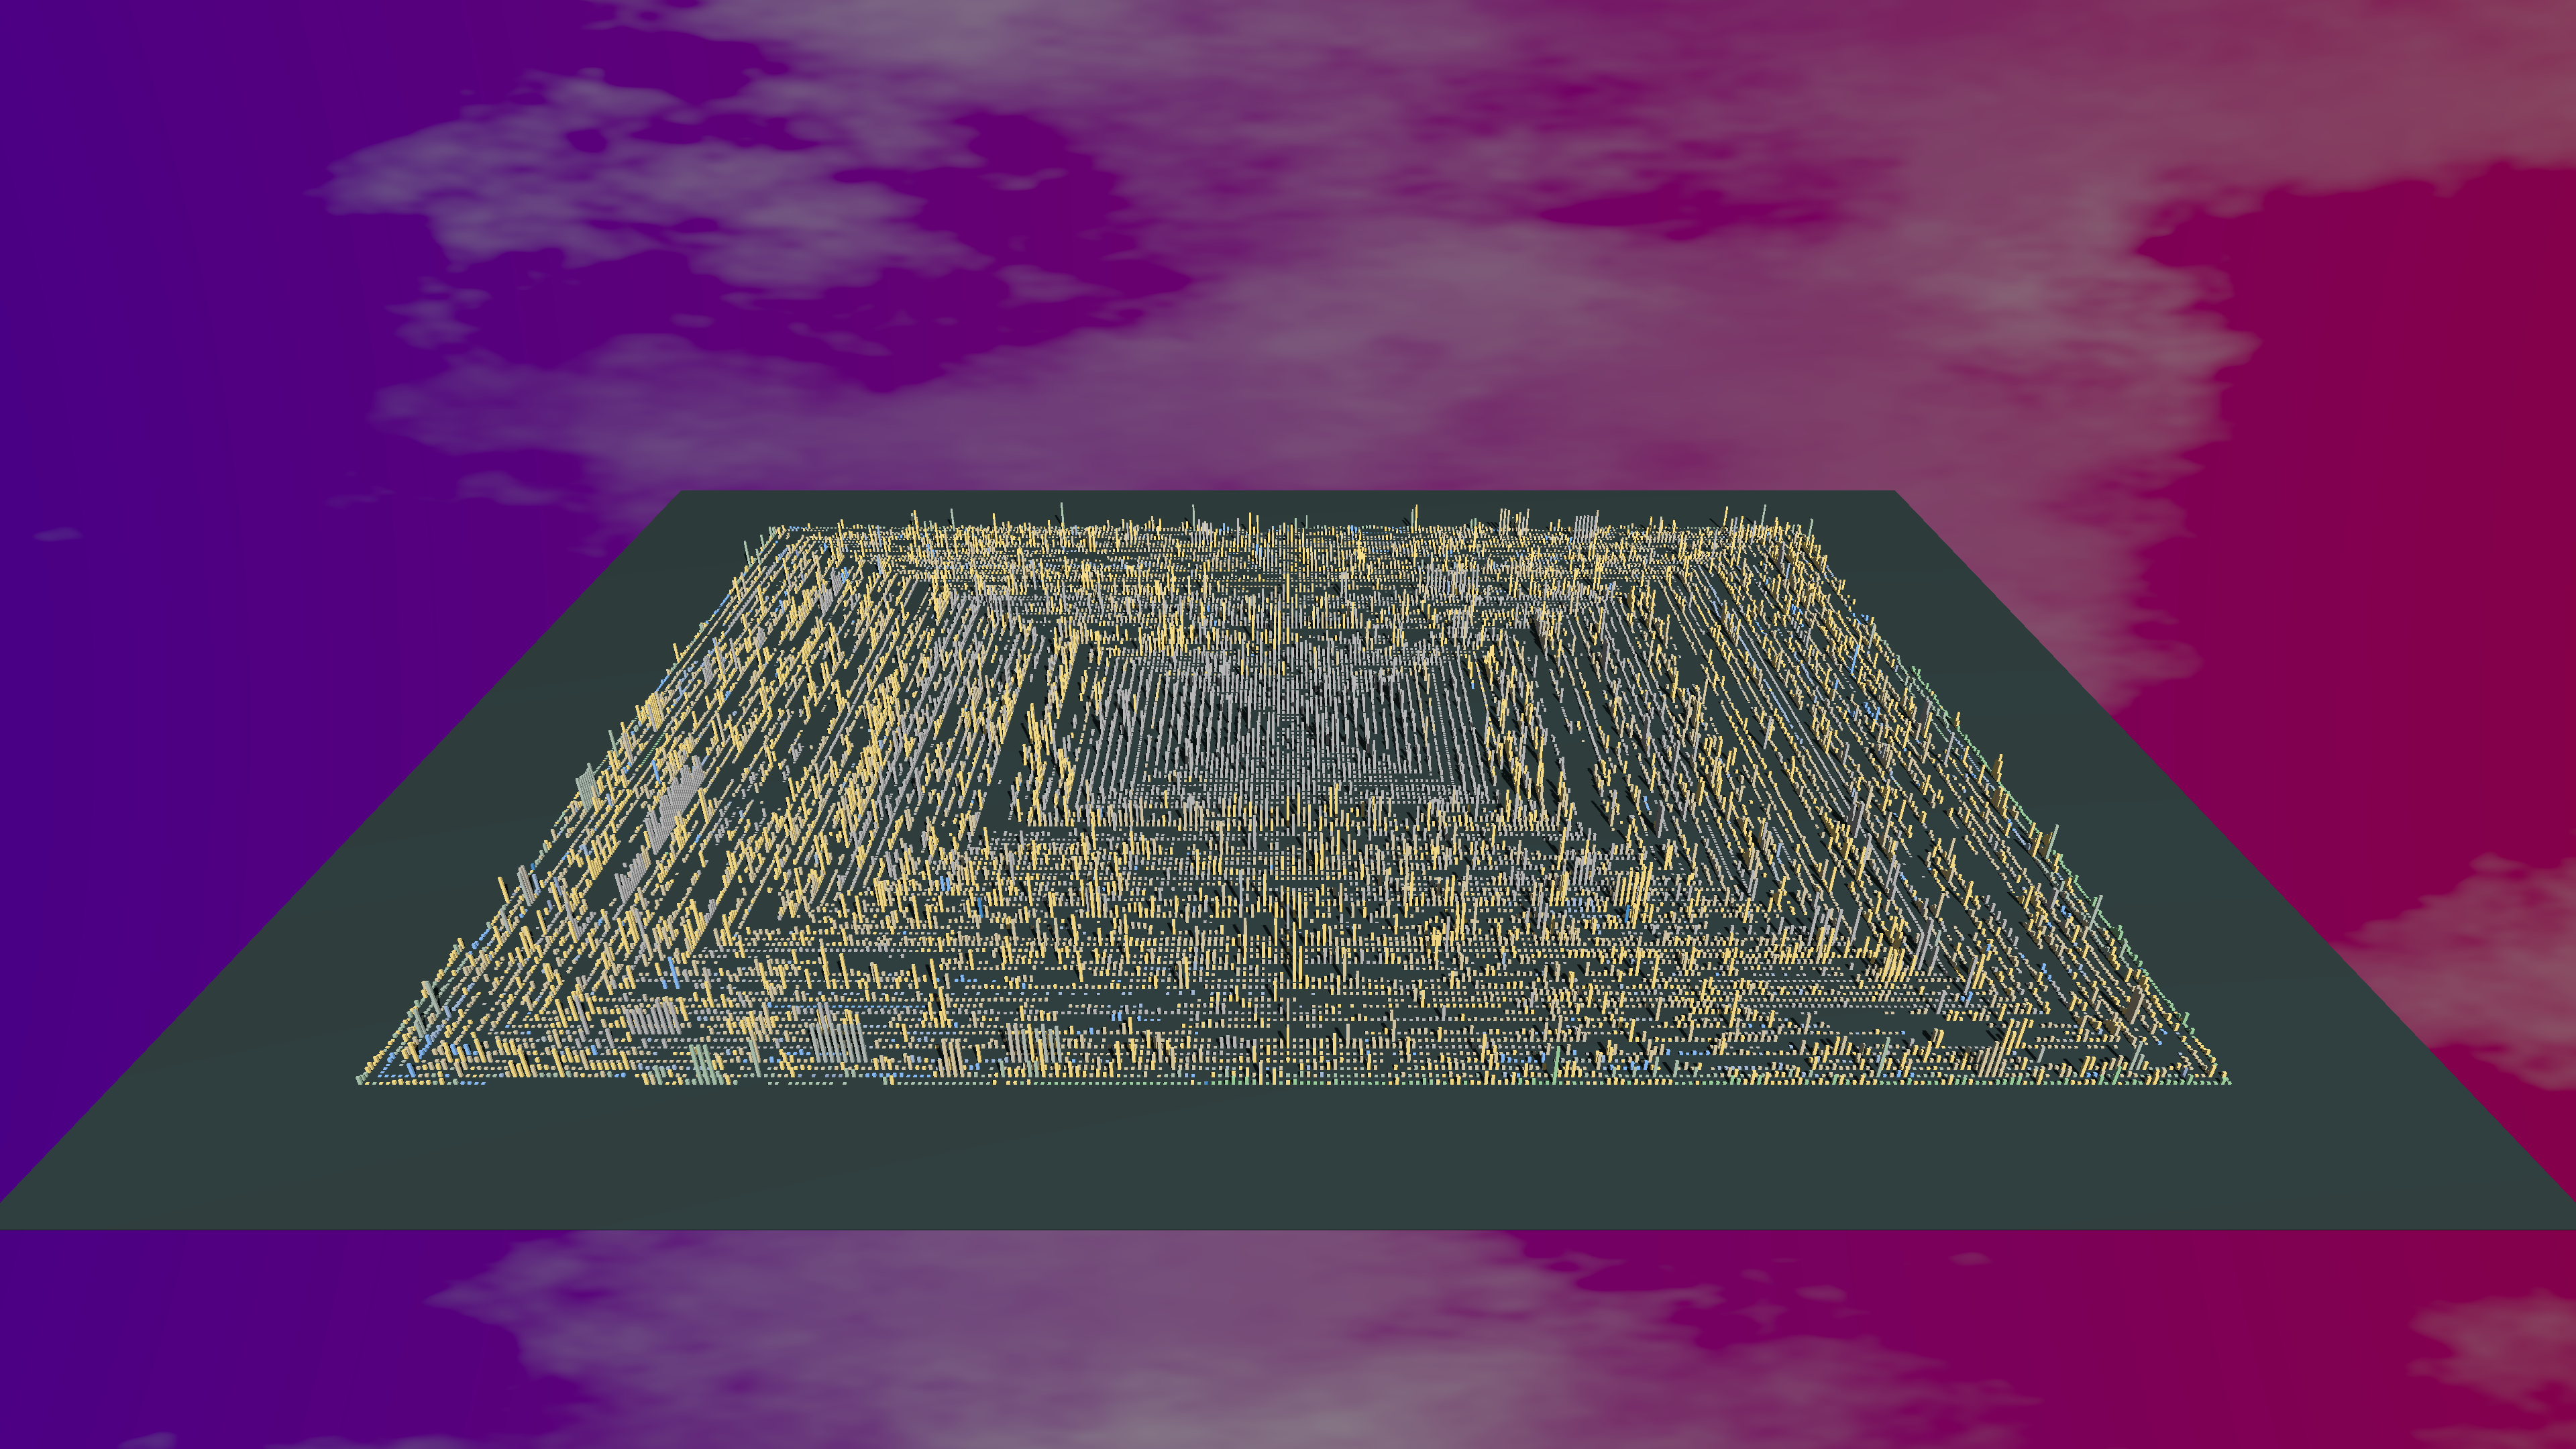
\includegraphics[width=\linewidth]{Elasticsearch/Animation008.png}
        \caption{Elasticsearch in June 2021 (8 year)} 
        \label{fig:Elastic_V5_S5}
    \end{subfigure}\hspace*{\fill}
    \begin{subfigure}{0.48\textwidth}
        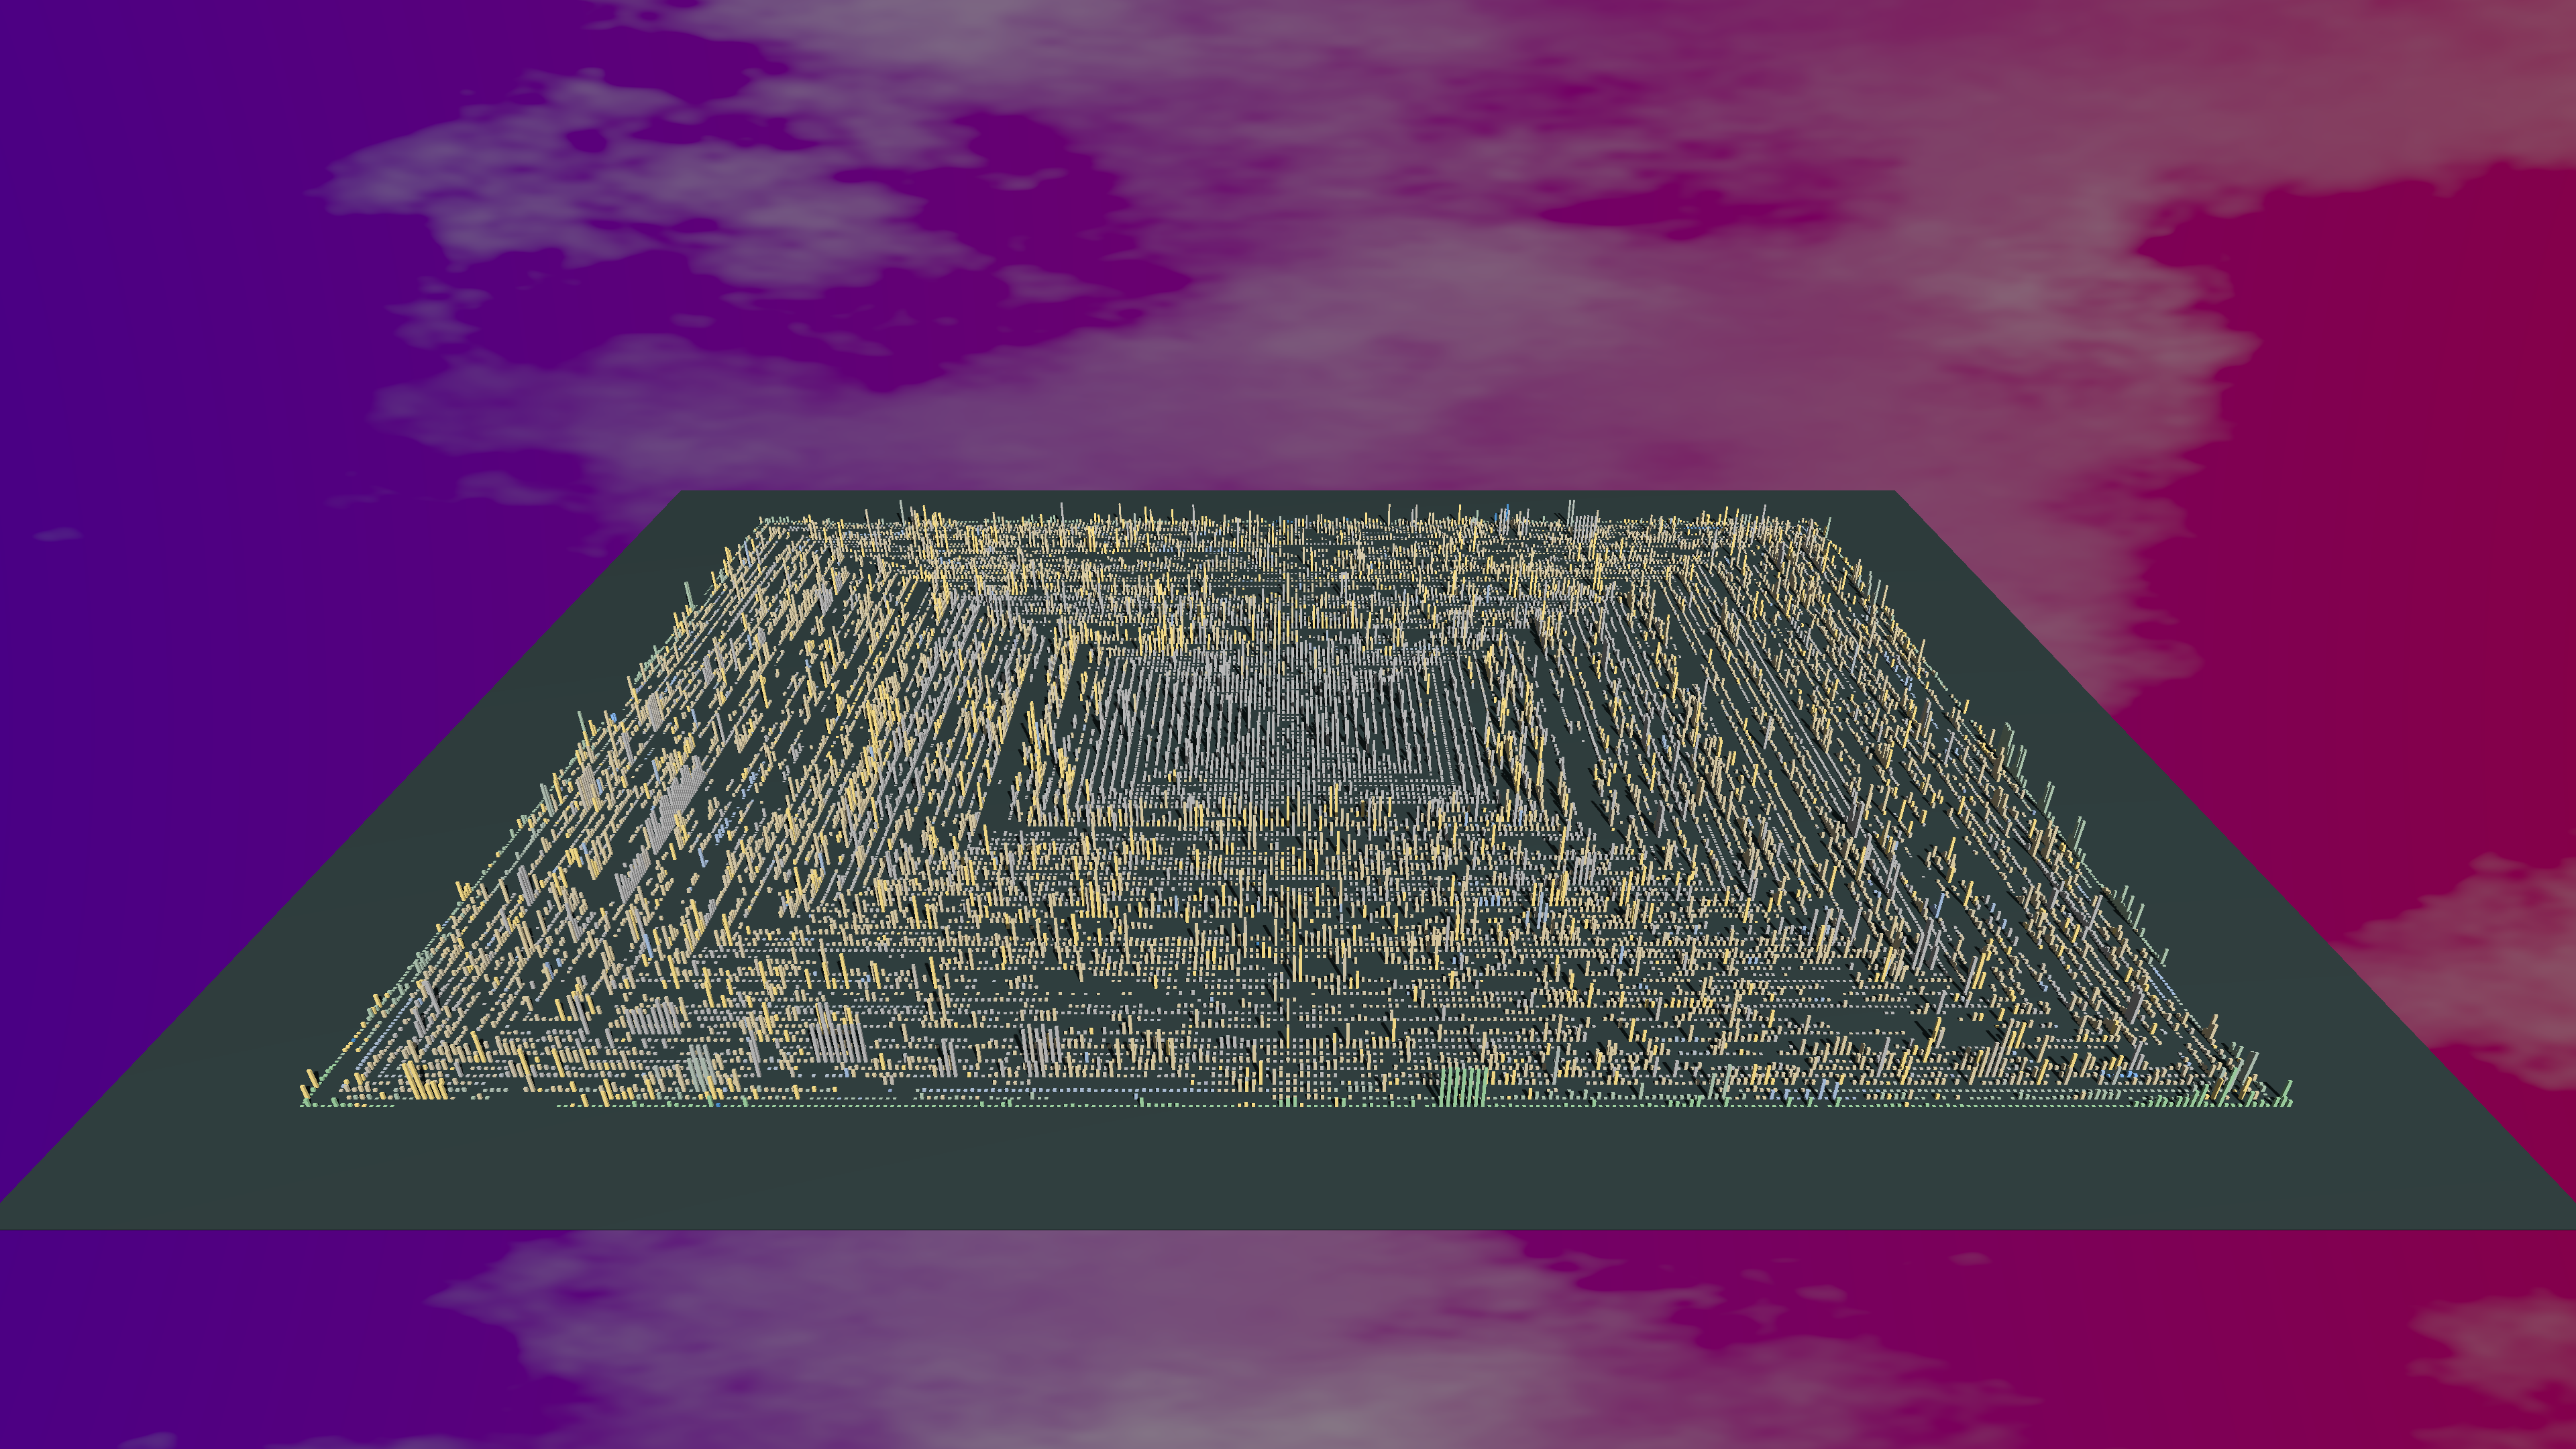
\includegraphics[width=\linewidth]{Elasticsearch/Animation009.png}
        \caption{Elasticsearch in June 2022 (9 year)} 
        \label{fig:Elastic_V5_S6}
    \end{subfigure}
    
    \caption{Hot spots during the evolution of Elasticsearch} 
    \label{fig:Elastic_V5}
\end{figure}


% -------------------------------------------
% libreoffice
% FileHistories: 213791 
% ProjectVersions: 367996 
% FileVersions: 1924183 
% First Version: 
% 	 hash: 5acbb755f3f8dedf51904b711ff78f5e1aa498cf 
% 	 date: Thu Mar 07 16:45:23 CET 2002 
% Last Version: 
% 	 hash: 634f13a722dc68b7a2df7518880ce4f9d5d89f19 
% 	 date: Sat Jun 18 16:10:53 CEST 2022 
% Diff: {DAYS=107, HOURS=22, MINUTES=25, SECONDS=30, MILLISECONDS=0, MICROSECONDS=0, NANOSECONDS=0, YEARS=20}
% -------------------------------------------
\clearpage
\section{LibreOffice – 200K Files in 20 Years}
LibreOffice is an integrated office suite compatible with most document formats and standards. Its first commit,\footnote{\url{https://github.com/LibreOffice/core/commit/5acbb755f3f8dedf51904b711ff78f5e1aa498cf}} made on March 7, 2002, was an import of the original codebase developed by Sun Microsystems. The repository's history is 20 years long, with 327,996 commits, 213,791 FileHistories, and almost 2M FileVersions. 

\bigbreak
%\subsection{View 6}
\textbf{Visualization goal:}
This visualization aims to see how the repository evolved through its last 20 years. We adopt a commit grouping strategy based on a time window of one year and an aging strategy of one month with 12 steps. Hence, grey entities represent files that have not been updated for more than 12 months. 


View specification adopted: 
\begin{itemize}
    \item \texttt{versionGroupingStrategy}: timestamp.
    \item \texttt{versionGroupingChunkSize}: 31,556,926 (1 year). 
    \item \texttt{colorPalette}: default.
    \item \texttt{agingGroupingStrategy}: timestamp.
    \item \texttt{agingStepSize}: 2,629,743 (1 month).
    \item \texttt{agingSteps}: 12 steps.
    \item \texttt{mapperMetricName}: SIZE. 
    \item \texttt{fileTypeShape}: all BOX. 
    \item \texttt{fileTypeOpacity}: all 1. 
\end{itemize}

\textbf{Results:}
We present only the relevant aspects of the evolution that we have found. The full evolution is depicted in \autoref{app:Libre_Evolution}. \autoref{fig:Libre_V6} shows the hot spots during the system's evolution. The initial composition of the system is shown in \autoref{fig:Libre_V6_S1}. Between 2003 and 2011, the system 
grew substantially. In March 2003, it had 13,500 files, and in March 2011, it had 57,520 files with an increment of over 40K files. \autoref{fig:Libre_V6_S2} shows the state of the repository in March 2011. Few entities are painted with a color, meaning that only a few parts of the codebase were touched. \autoref{fig:Libre_V6_S3} shows the state in March 2012. Closely to that date, the repository undergoes a big refactoring where most of the recently added files were moved. In this picture, we initially start to see empty rings like in the analysis of ArgoUML. Another important aspect of this picture is that the core was entirely modified. As we can see, it is yellow, and the entities are taller than the year before. The work on the repository was constant until June 2022. In all the AnimationFrames, the center was always painted with yellow colors. This could mean that the core still needs maintenance after 20 years, recently developed features heavily rely on the core implementation. In the last 12 years, as can be seen in \autoref{fig:Libre_V6_S4}, \autoref{fig:Libre_V6_S5} and \autoref{fig:Libre_V6_S6} the system doubled its size. In June 2022, it counted 135,793 files. Empty rings around the core became thicker, suggesting the deletion of a significant part of the system which they probably reimplemented later.

\bigbreak
\textbf{Conclusion:} The evolution of LibreOffice was constant throughout its 20 years of history. 
Thanks to the aging concept of SYN, we understood that they heavily rely on code that was added 20 years ago. The core of the system was constantly updated, and the overall height of entities grew, especially in the middle. The empty rings around the core represent a pattern that we have already recognized in ArgoUML. It means that a set of files were removed one after another. Perhaps these files might be in an entire folder that contained a feature that was later readded. One issue that this visualization raised is regarding the size of the system. It is a limitation of this static approach because it is hard to infer the color of some entities since they are too small to be individually identified. An interactive tool like the Debugger module (\autoref{s:SYNDebugger}) would not have this limitation because it allows zooming. 


\begin{figure}[ht]
    \begin{subfigure}{0.48\textwidth}
        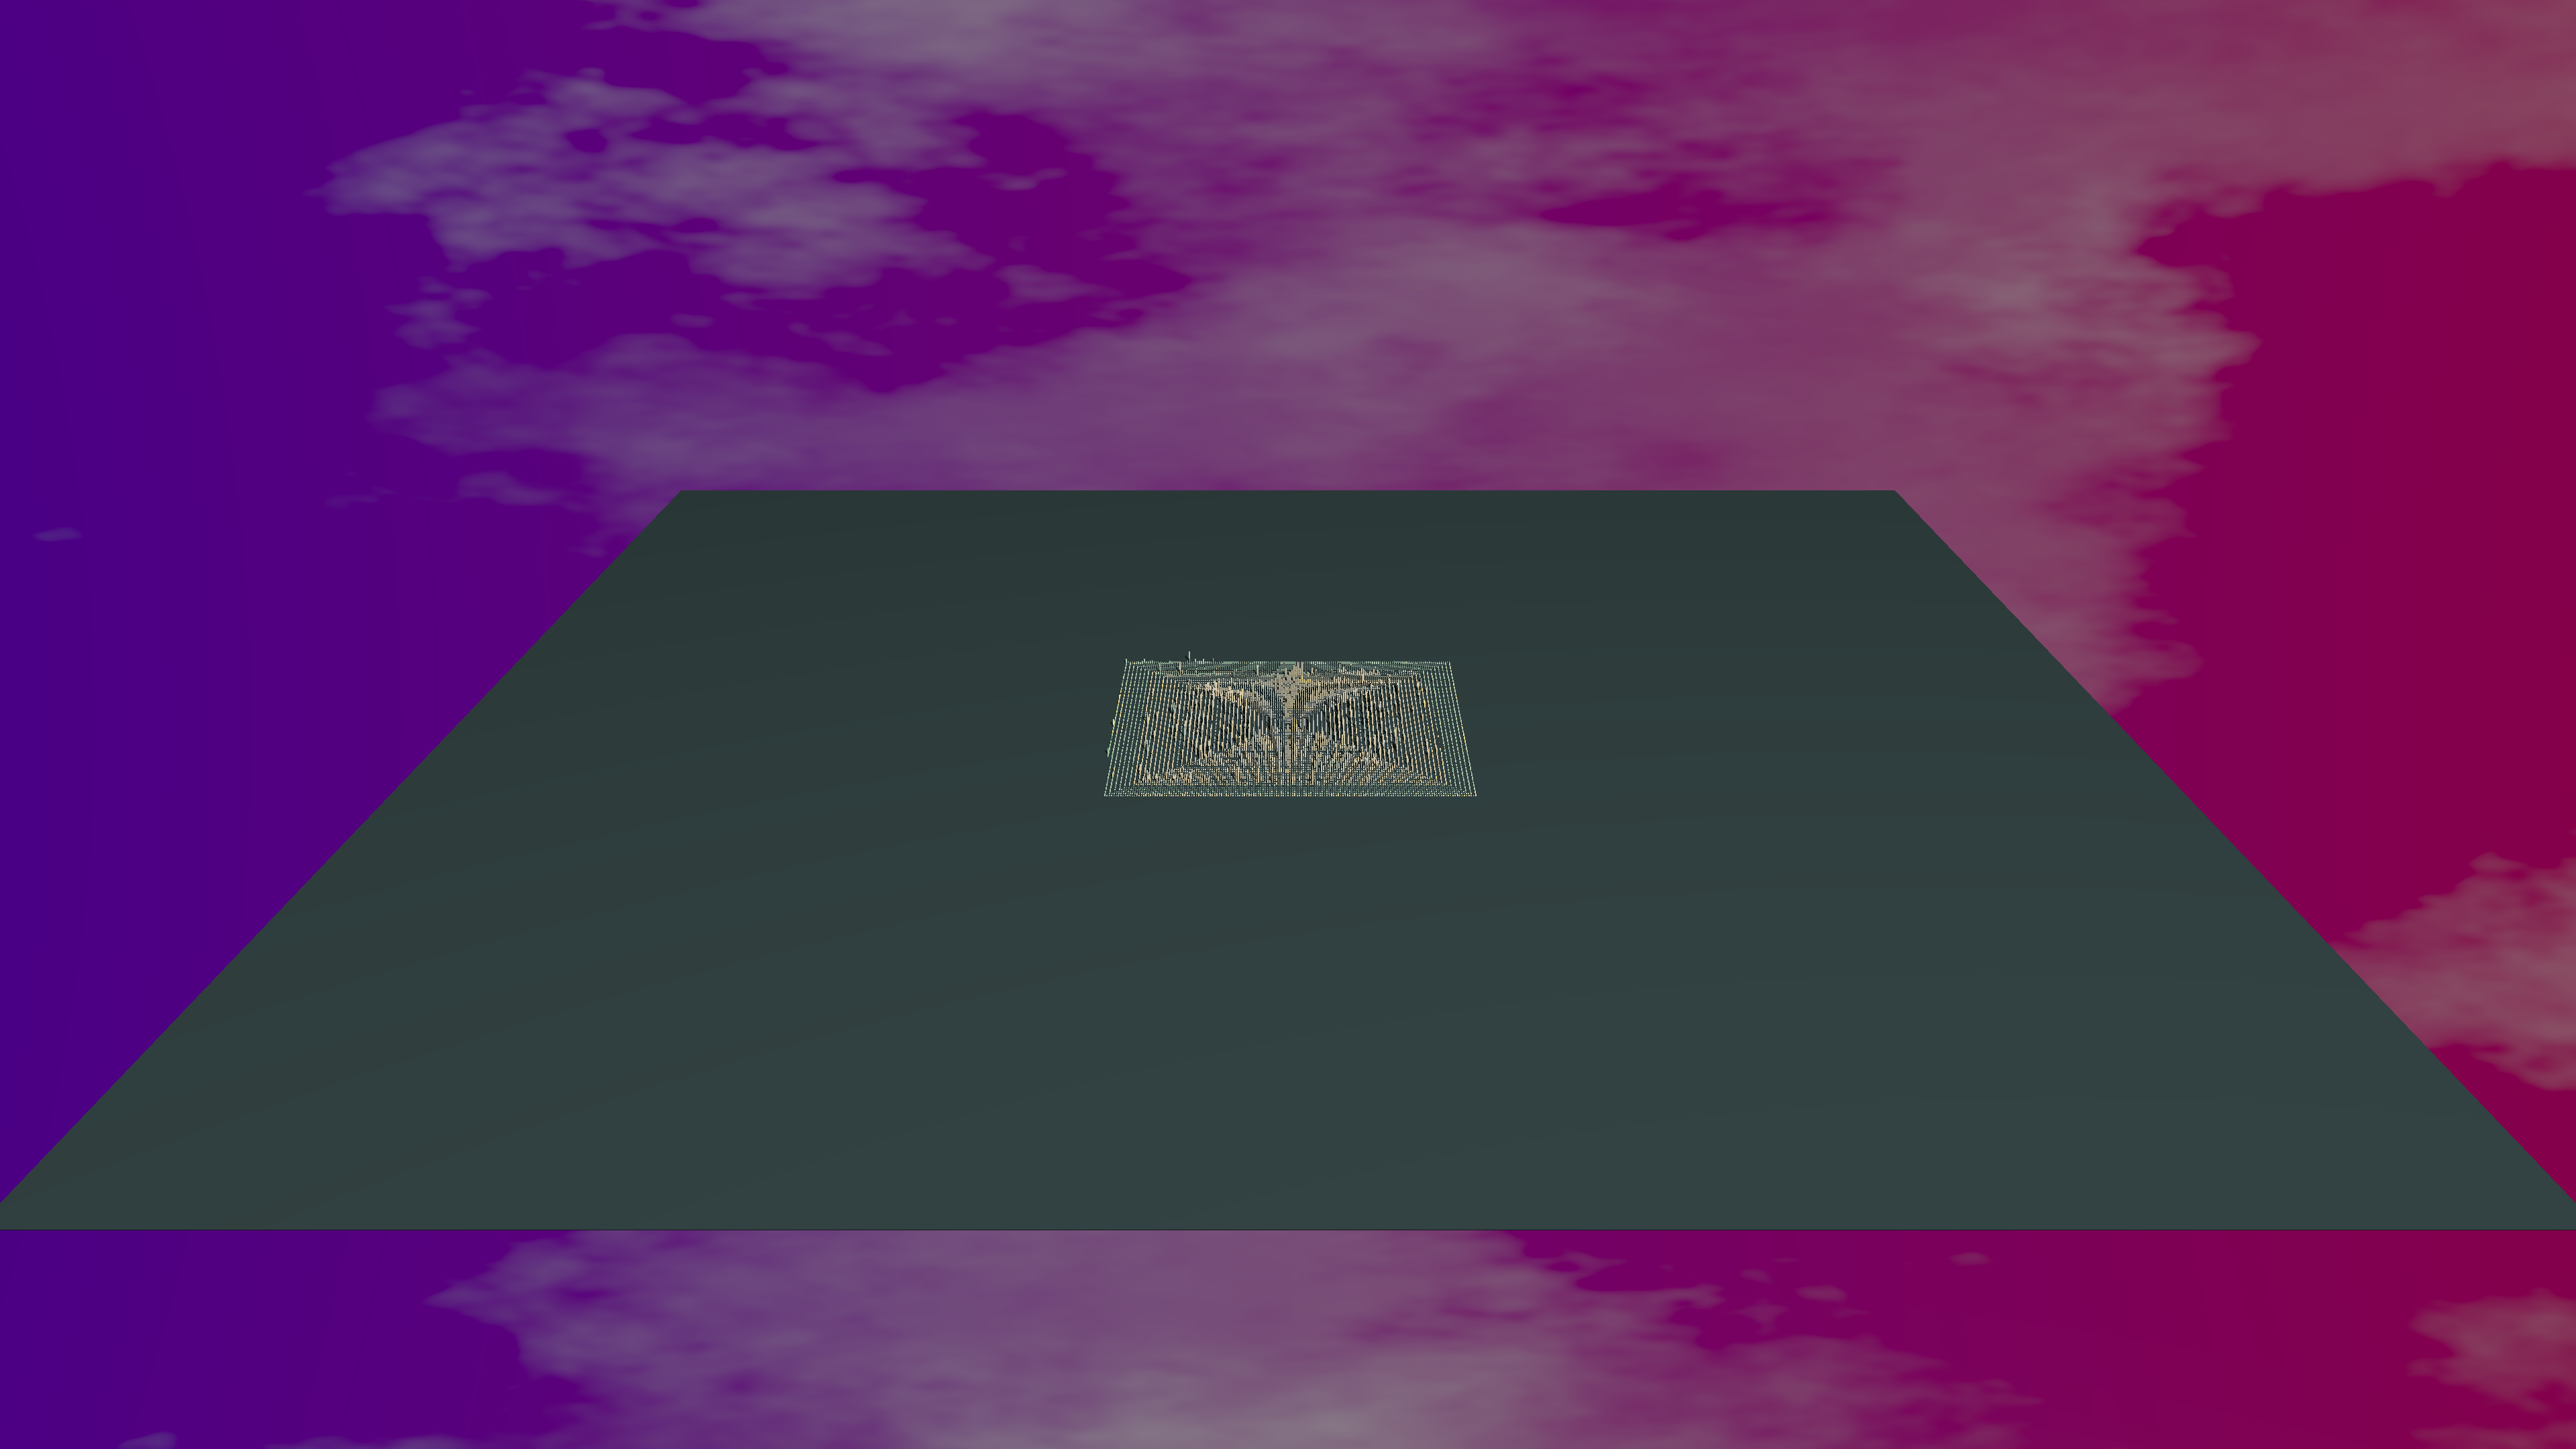
\includegraphics[width=\linewidth]{Libreoffice/Animation001.png}
        \caption{LibreOffice in March 2003 (1 year)} 
        \label{fig:Libre_V6_S1}
    \end{subfigure}\hspace*{\fill}
    \begin{subfigure}{0.48\textwidth}
        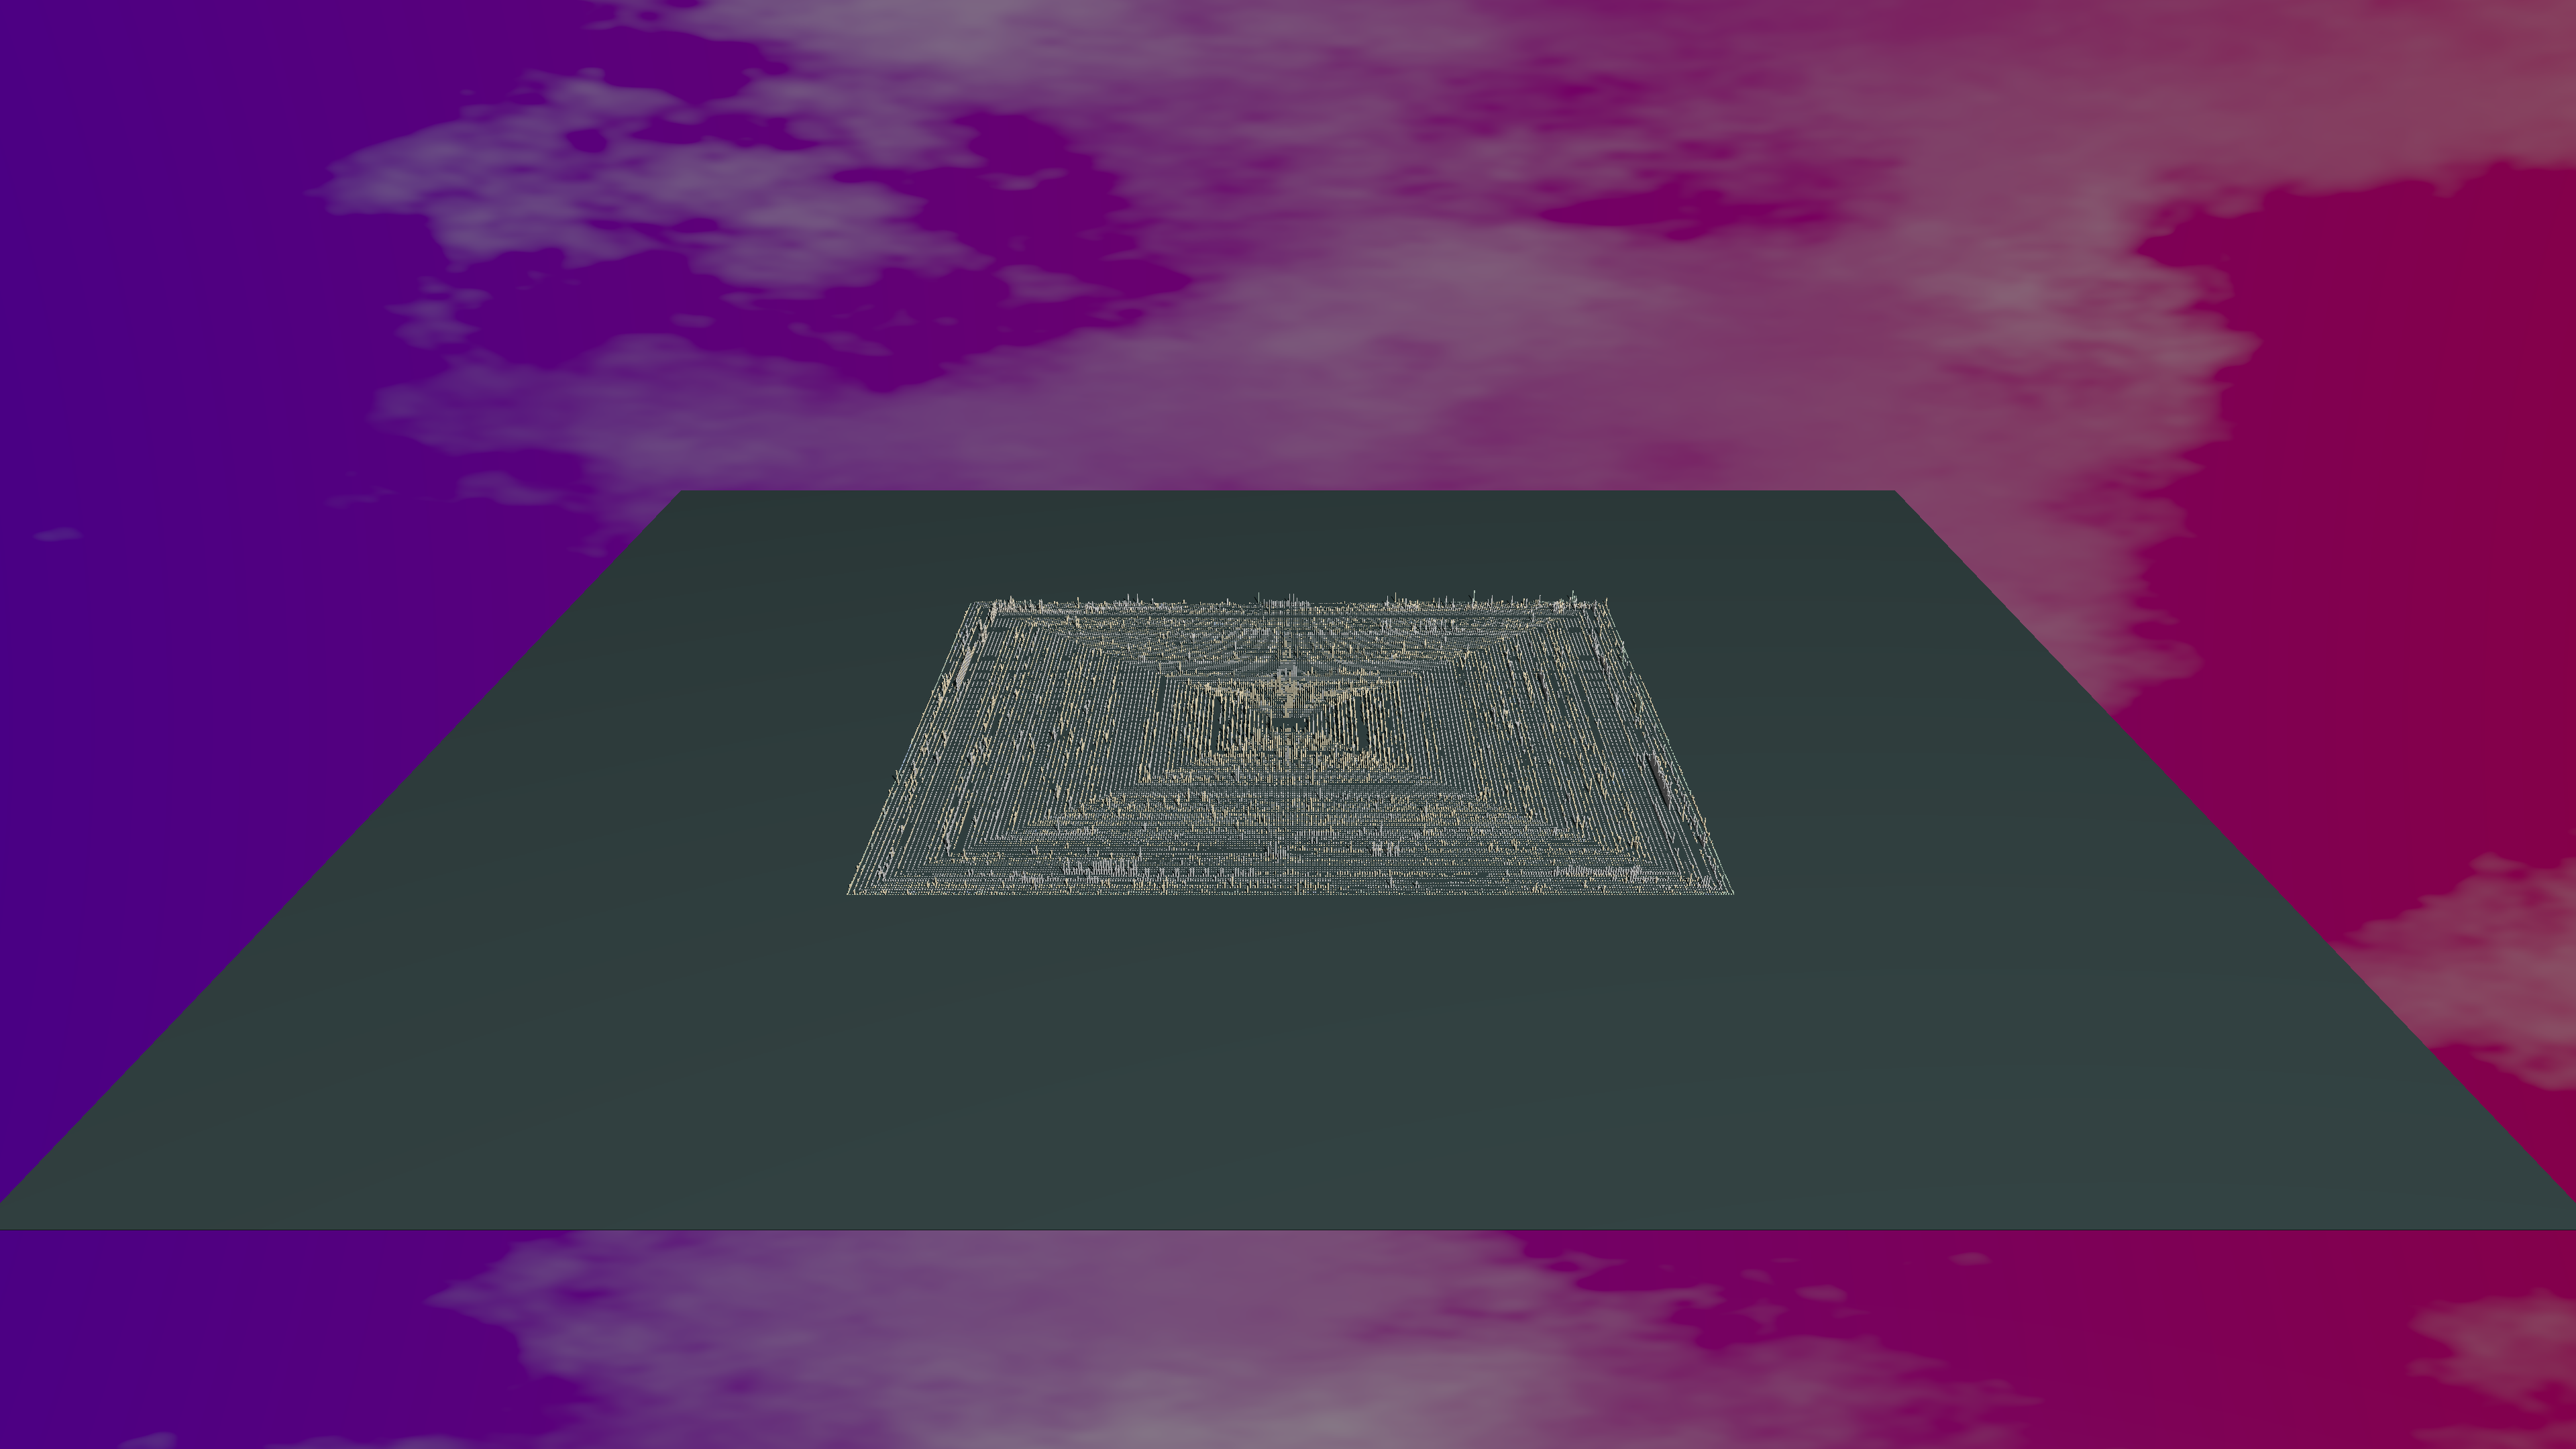
\includegraphics[width=\linewidth]{Libreoffice/Animation009.png}
        \caption{LibreOffice in March 2011 (9 year)} 
        \label{fig:Libre_V6_S2}
    \end{subfigure}
    \medskip
    \begin{subfigure}{0.48\textwidth}
        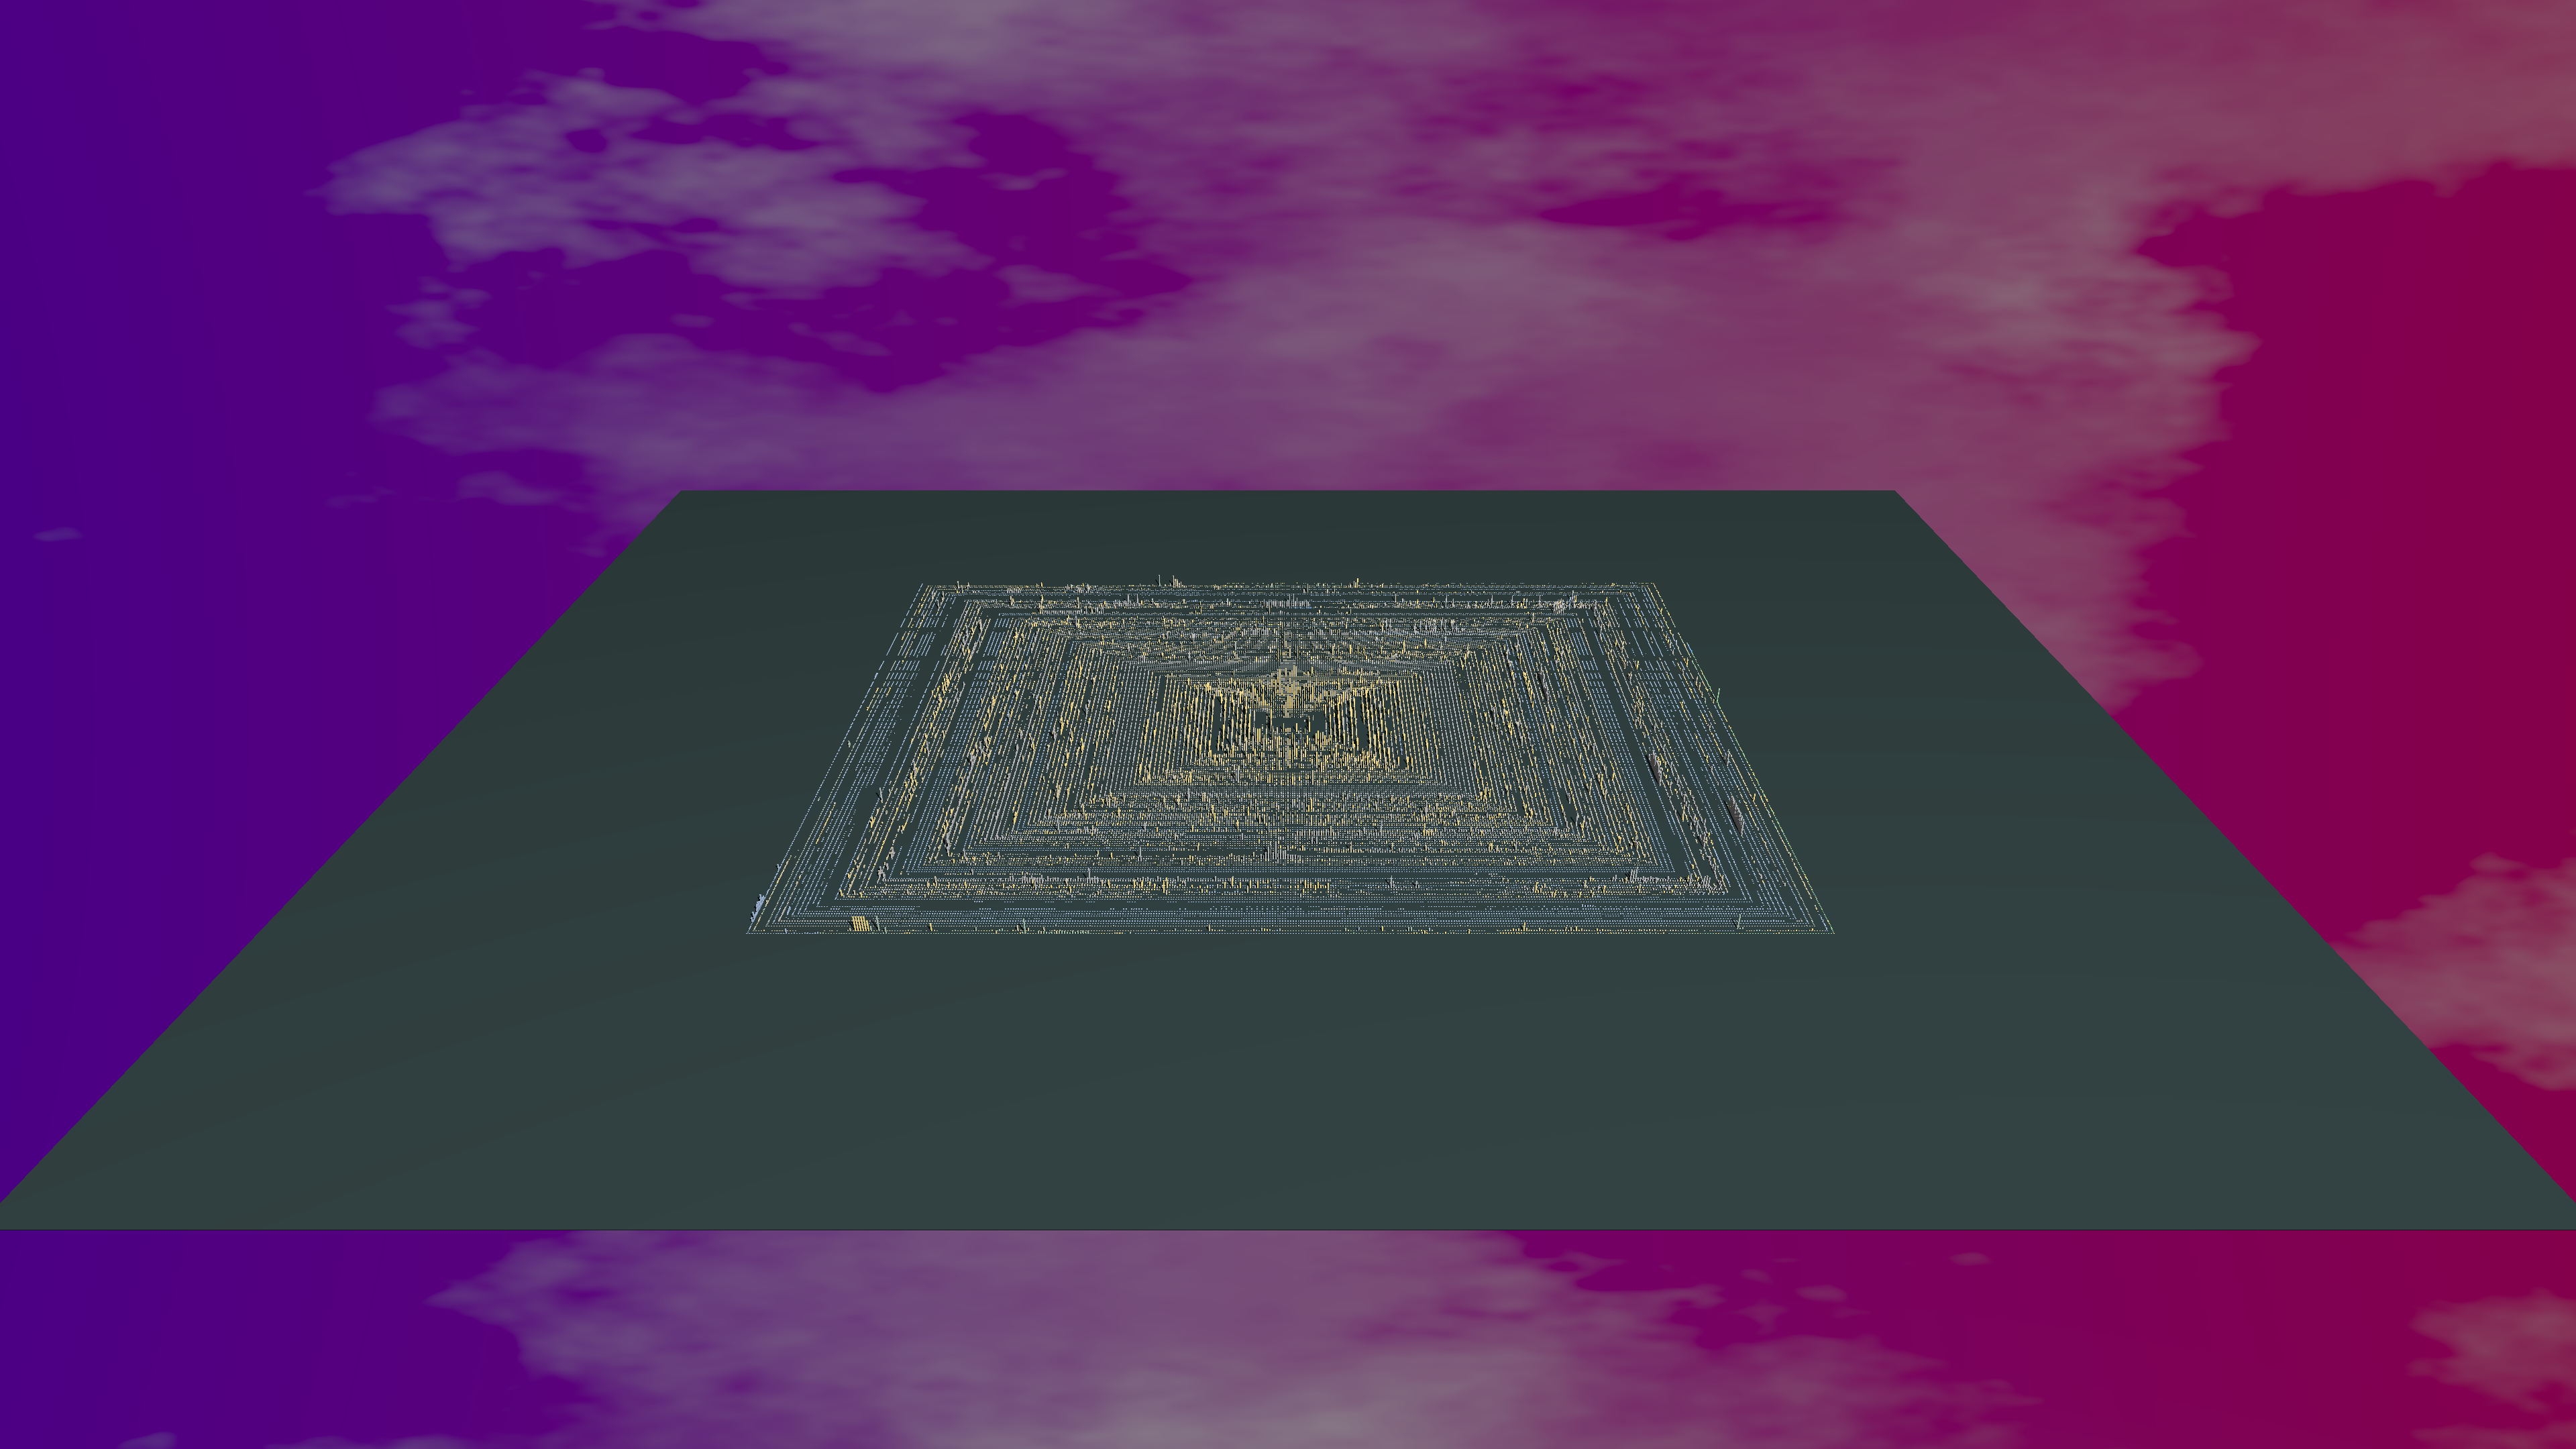
\includegraphics[width=\linewidth]{Libreoffice/Animation010.png}
        \caption{LibreOffice in March 2012 (10 year)} 
        \label{fig:Libre_V6_S3}
    \end{subfigure}\hspace*{\fill}
    \begin{subfigure}{0.48\textwidth}
        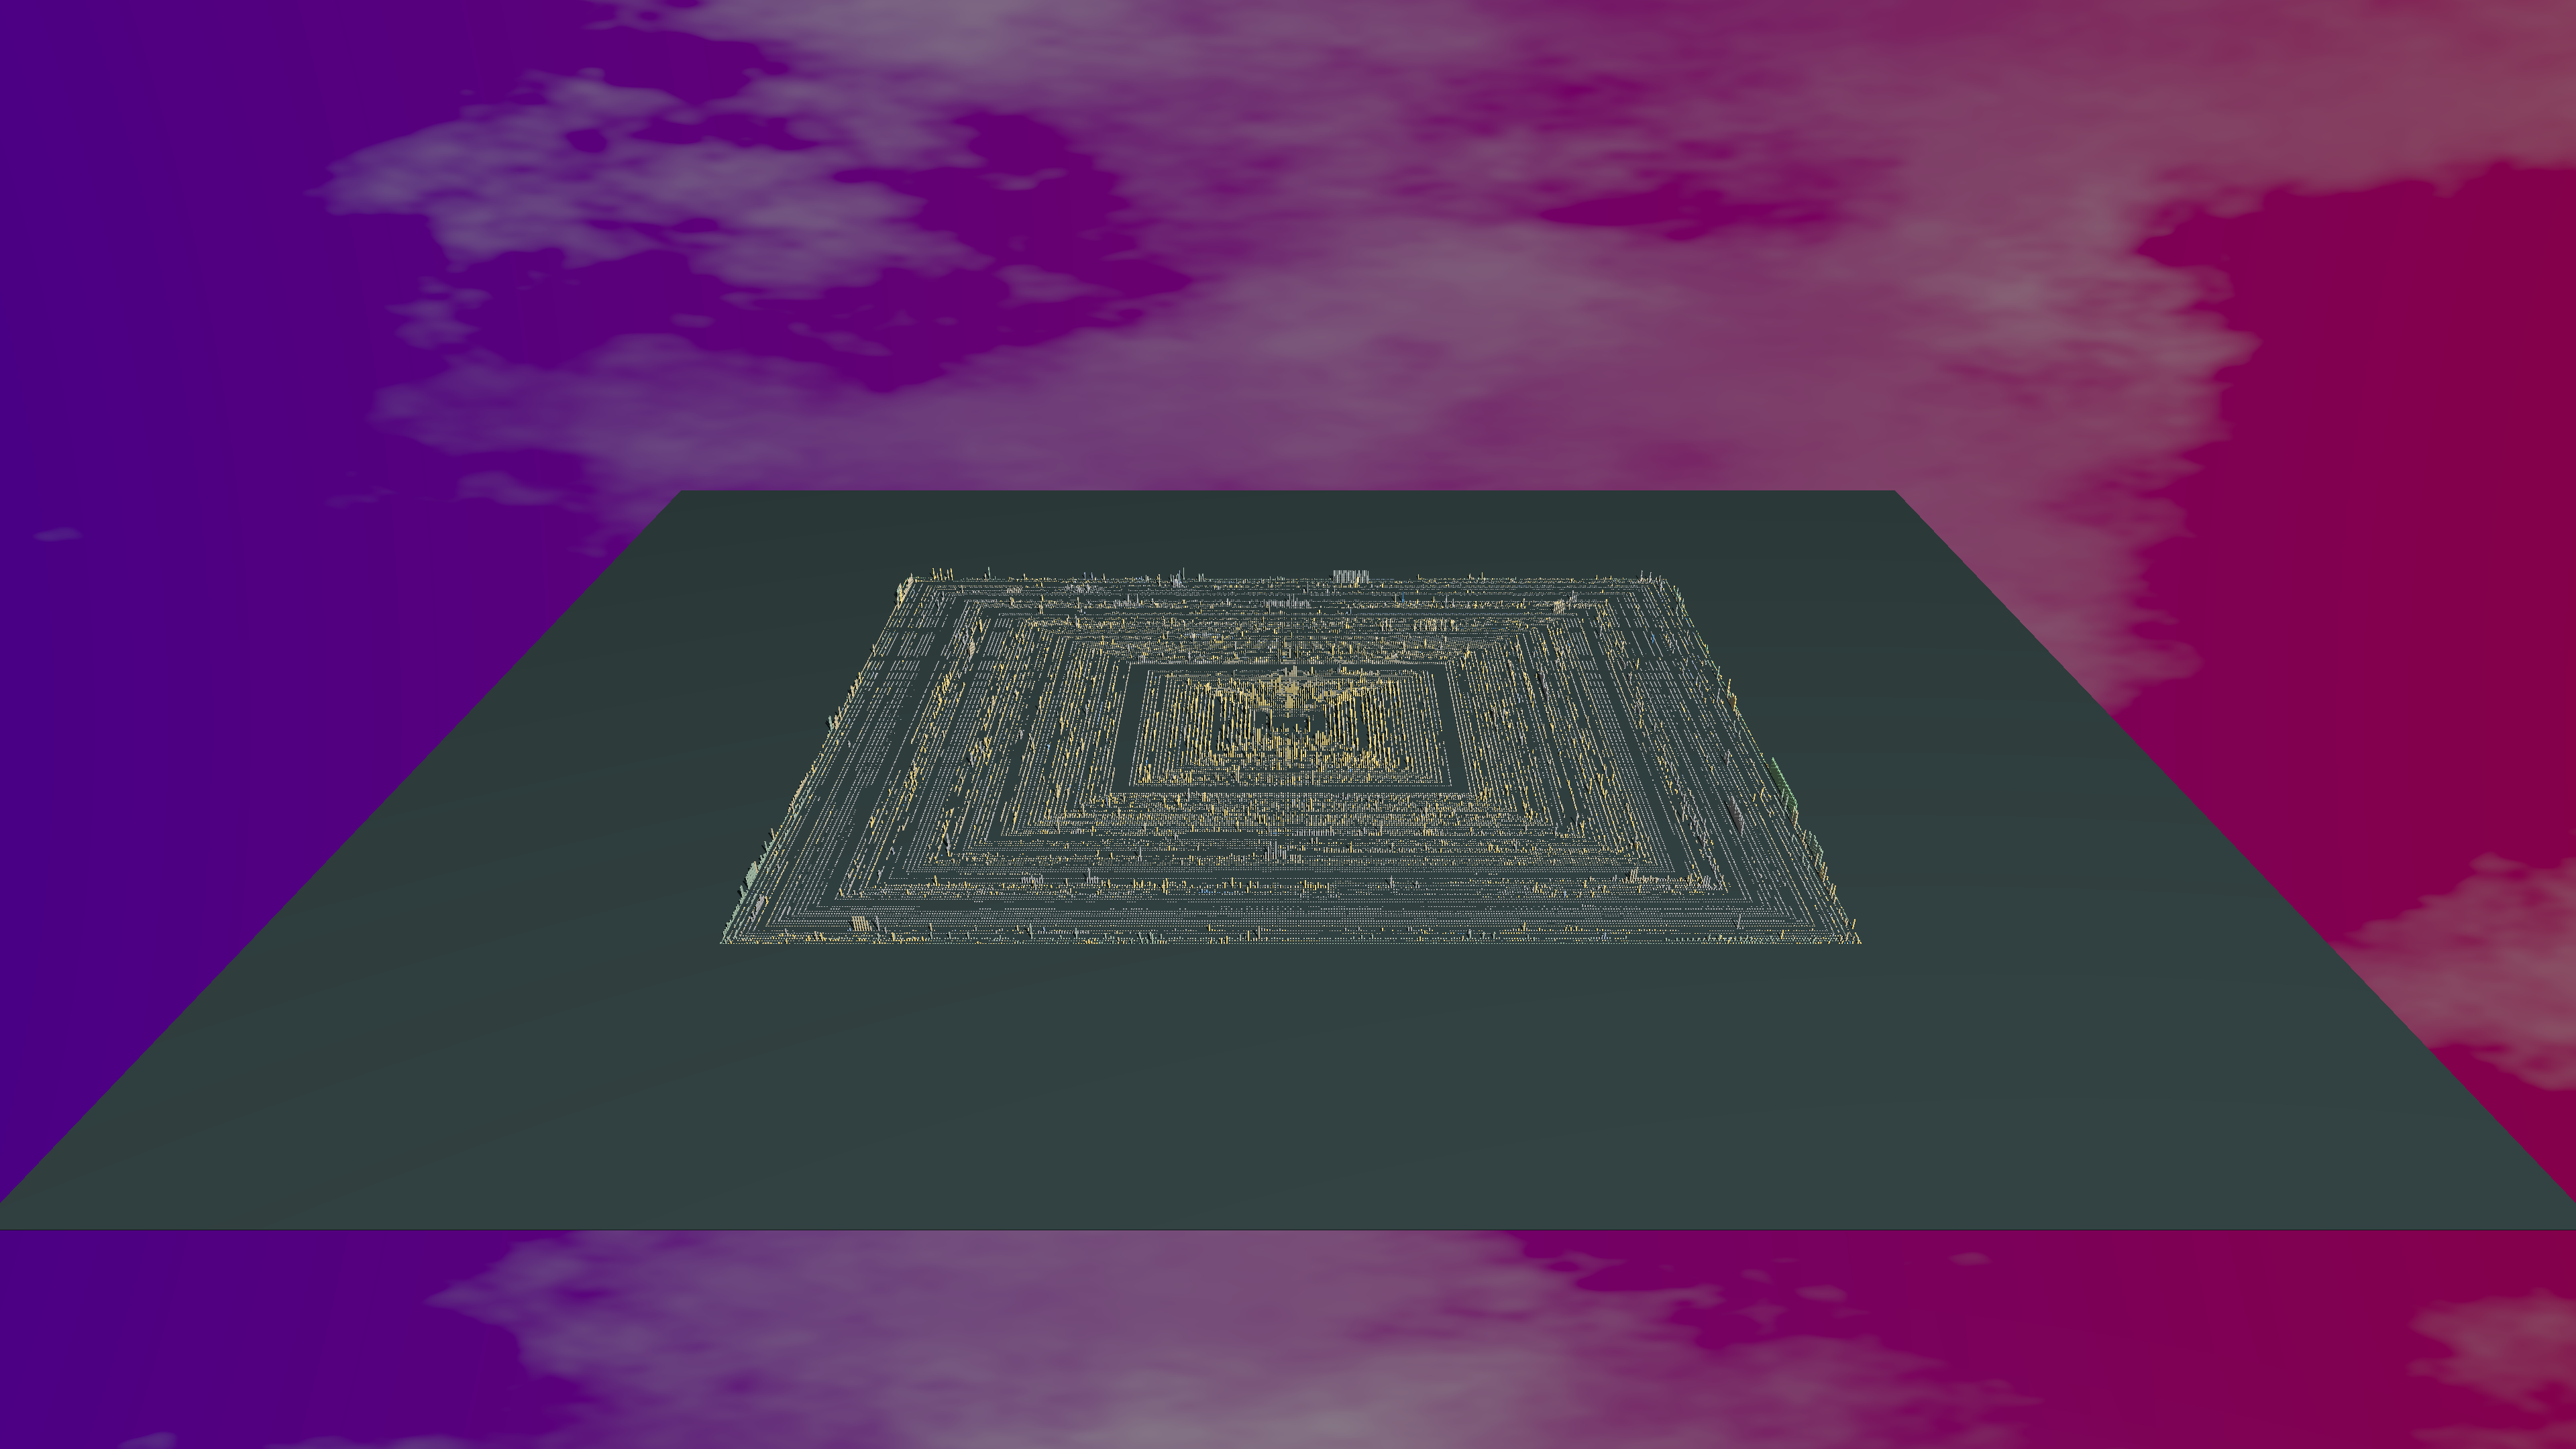
\includegraphics[width=\linewidth]{Libreoffice/Animation011.png}
        \caption{LibreOffice in March 2013 (11 year)} 
        \label{fig:Libre_V6_S4}
    \end{subfigure}
    \medskip
    \begin{subfigure}{0.48\textwidth}
        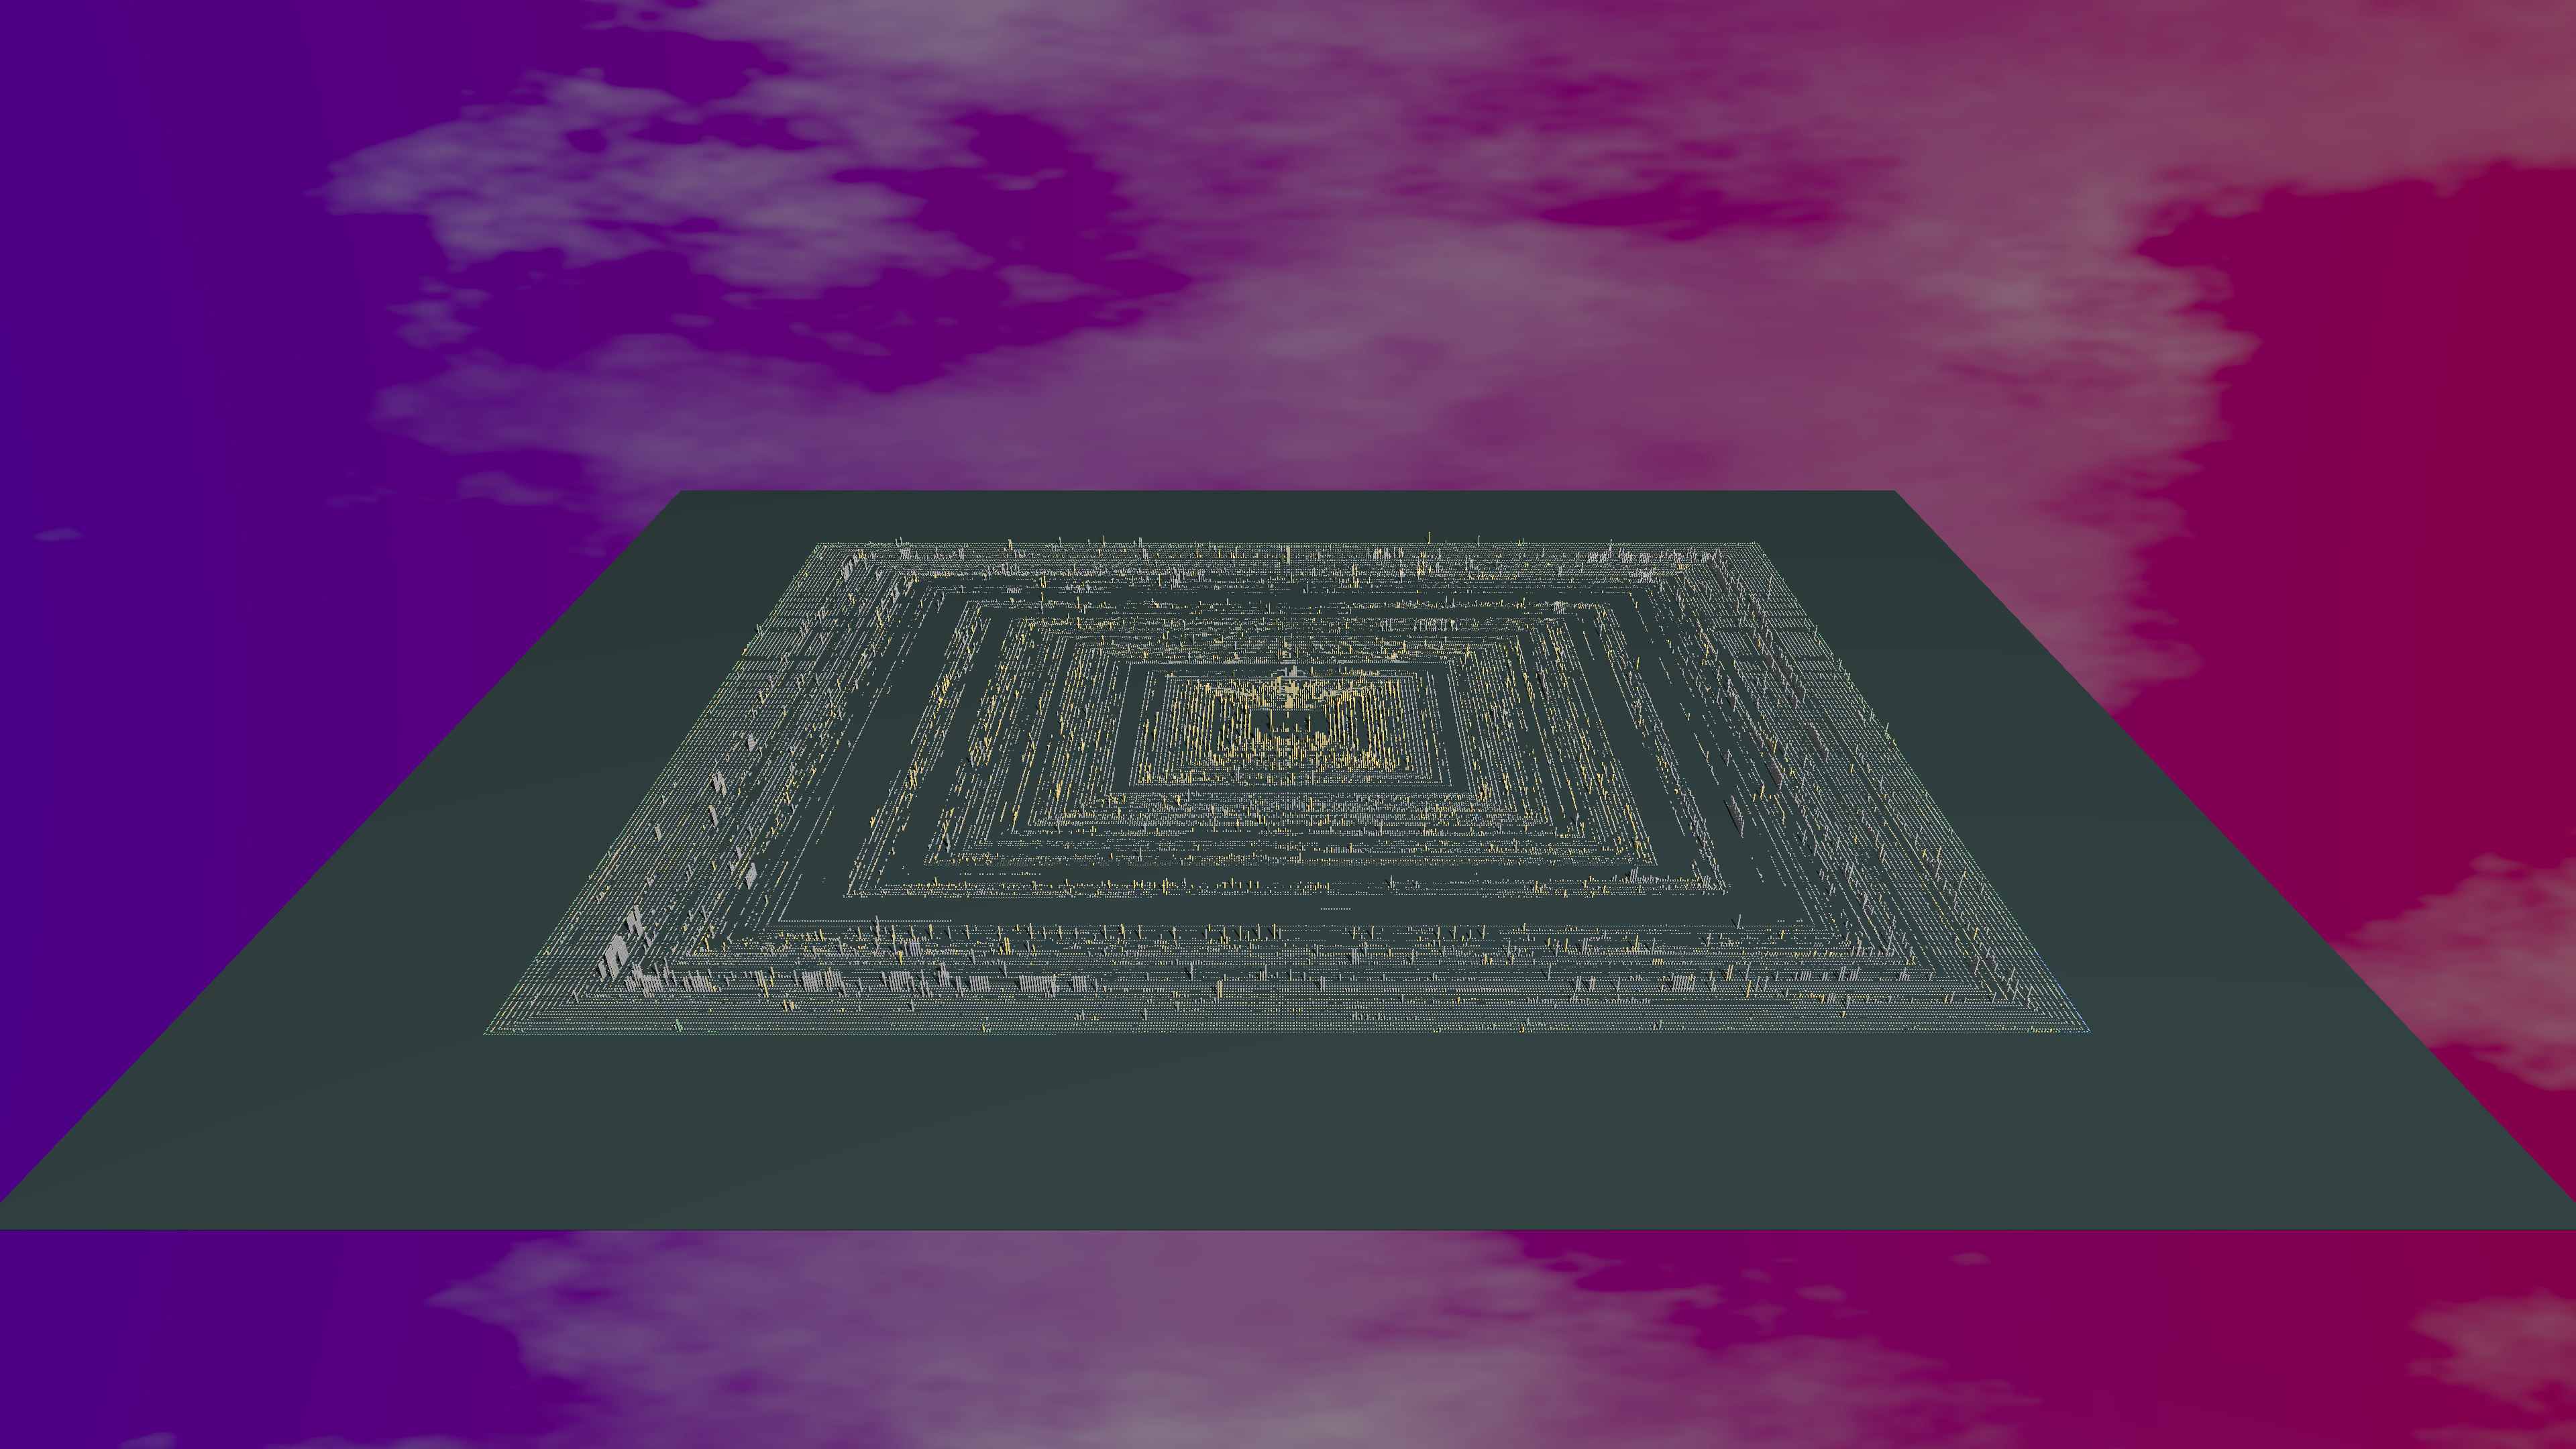
\includegraphics[width=\linewidth]{Libreoffice/Animation017.png}
        \caption{LibreOffice in March 2019 (17 year)} 
        \label{fig:Libre_V6_S5}
    \end{subfigure}\hspace*{\fill}
    \begin{subfigure}{0.48\textwidth}
        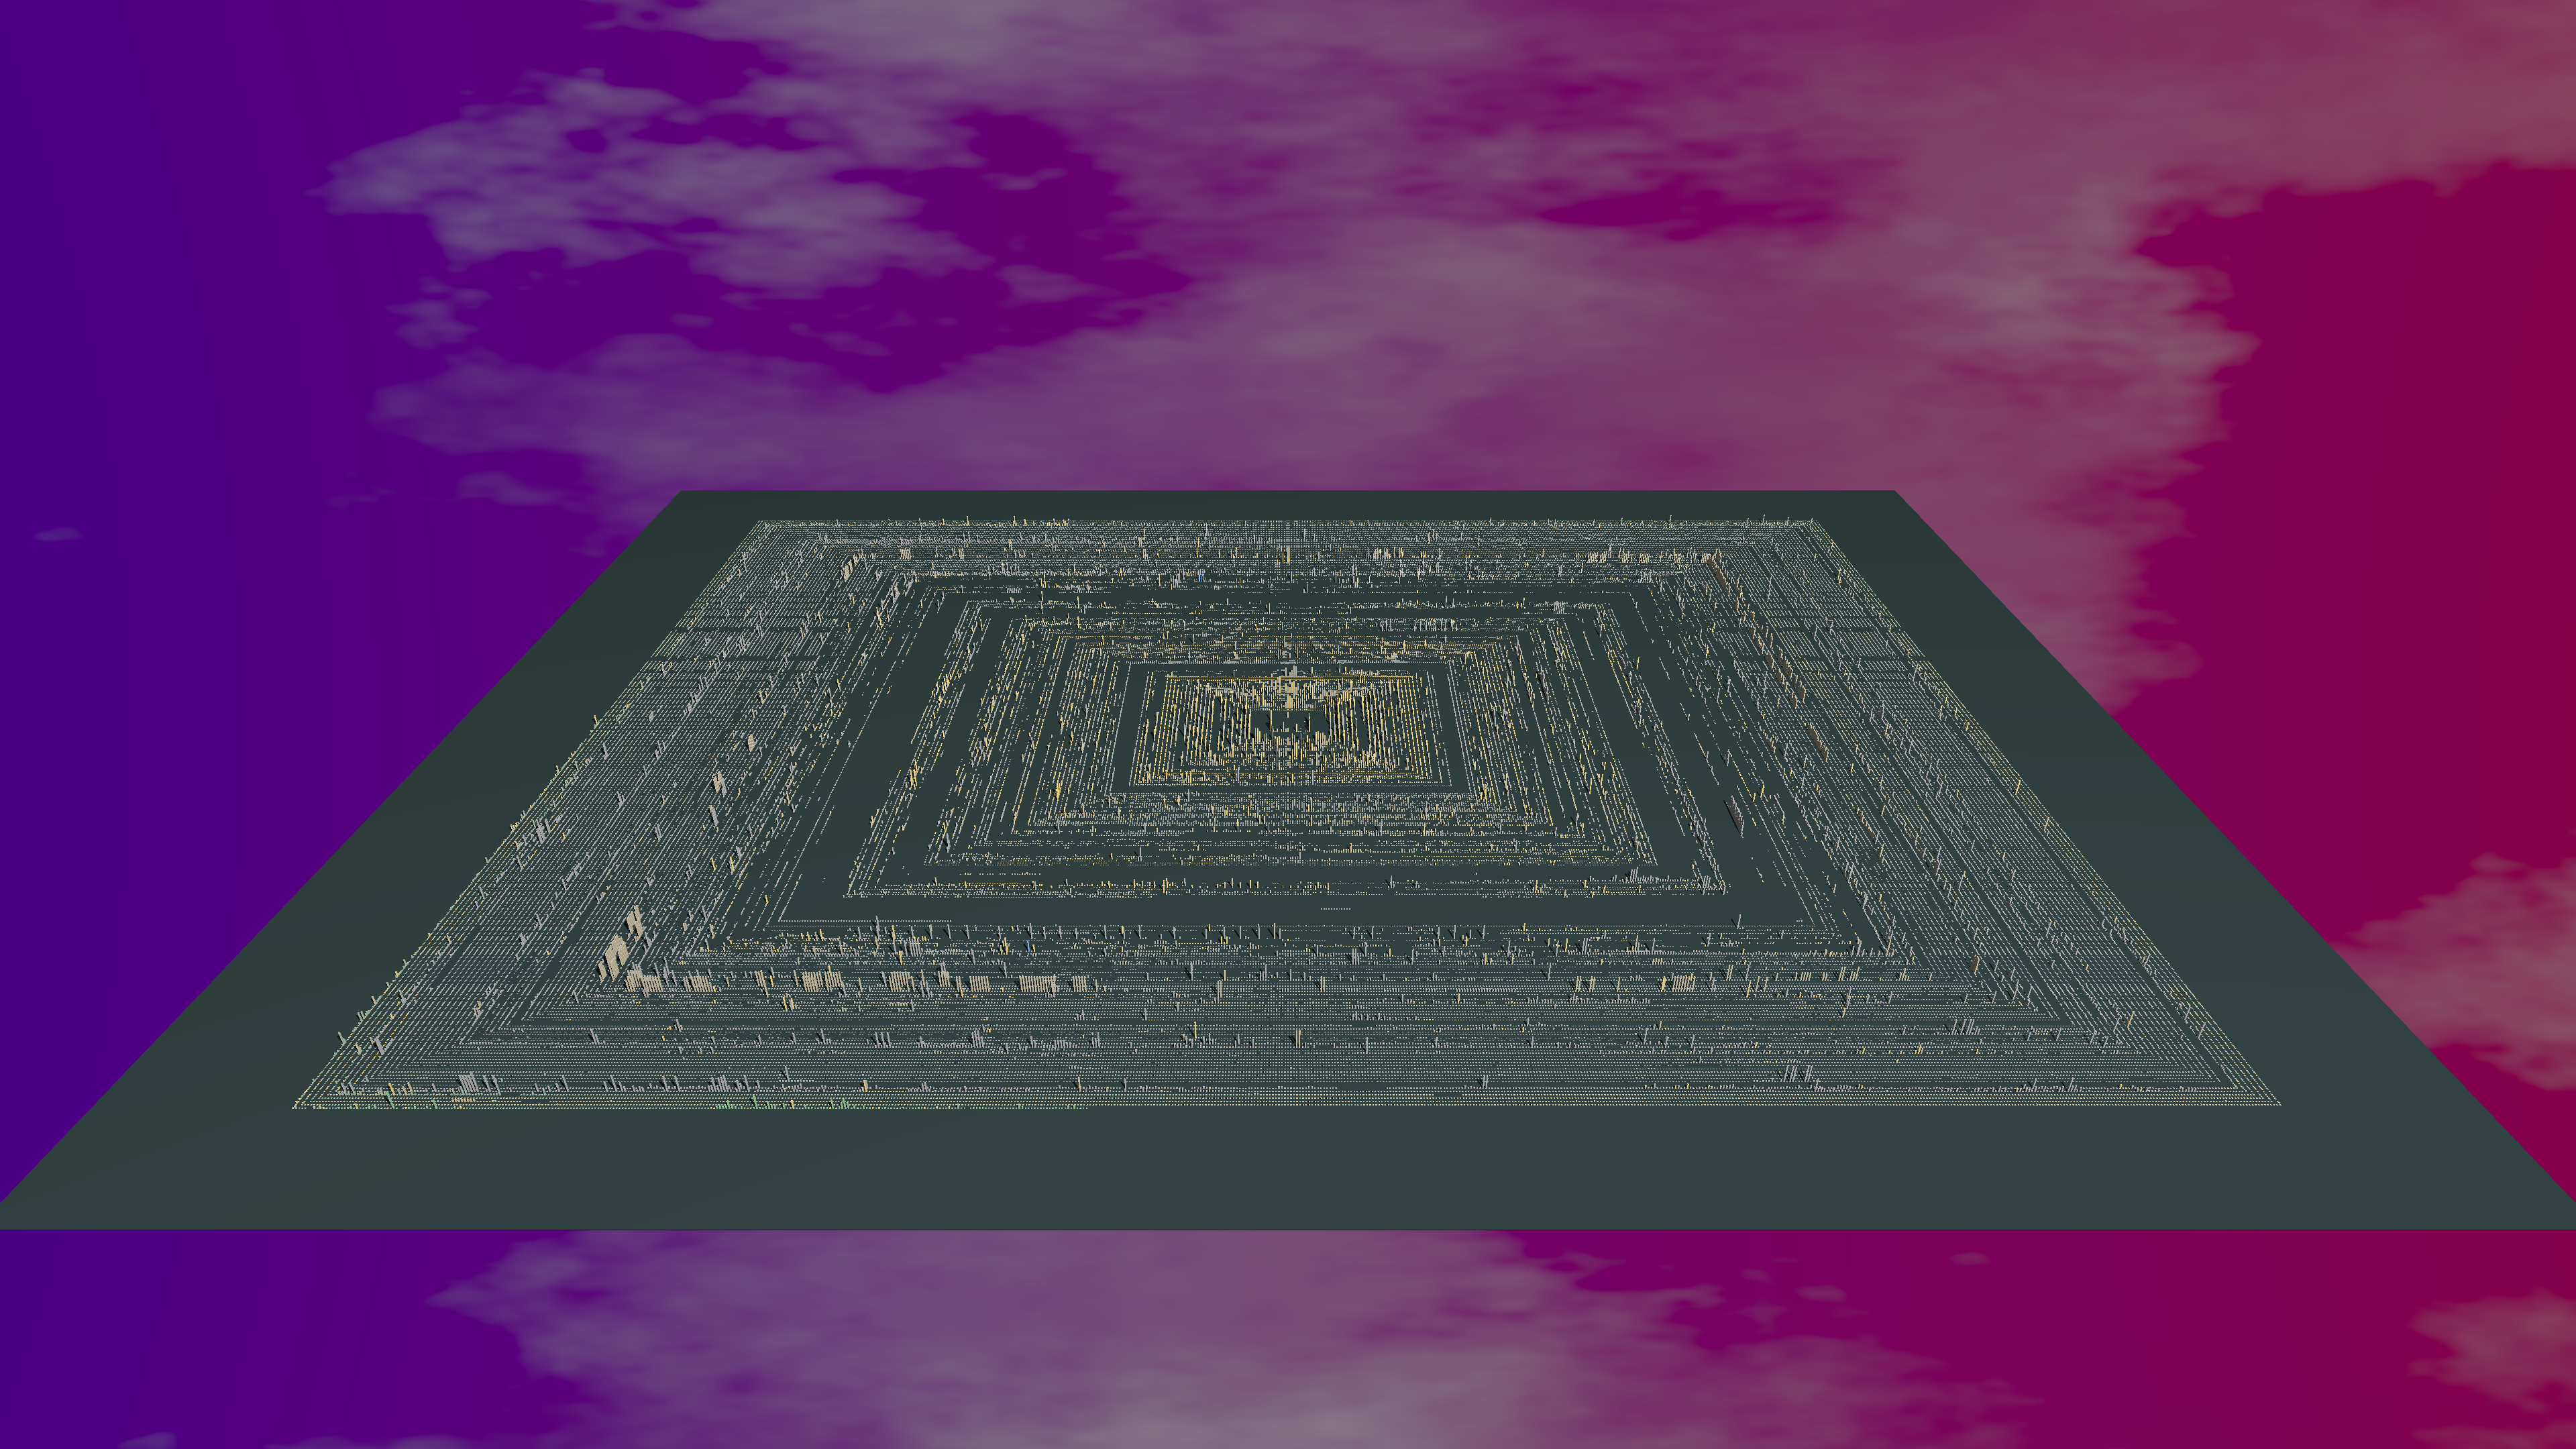
\includegraphics[width=\linewidth]{Libreoffice/Animation021.png}
        \caption{LibreOffice in June 2022 (21 year)} 
        \label{fig:Libre_V6_S6}
    \end{subfigure}
    
    \caption{Hot spots during the evolution of LibreOffice} 
    \label{fig:Libre_V6}
\end{figure}


% -------------------------------------------
% linux
% FileHistories: 109829 
% ProjectVersions: 997486 
% FileVersions: 2335535 
% First Version: 
% 	 hash: 1da177e4c3f41524e886b7f1b8a0c1fc7321cac2 
% 	 date: Sun Apr 17 00:20:36 CEST 2005 
% Last Version: 
% 	 hash: 705191b03d507744c7e097f78d583621c14988ac 
% 	 date: Tue Apr 19 19:19:02 CEST 2022 
% Diff: {DAYS=6, HOURS=18, MINUTES=58, SECONDS=26, MILLISECONDS=0, MICROSECONDS=0, NANOSECONDS=0, YEARS=17}
% -------------------------------------------
\clearpage
\section{Linux – Over a Million Commits}
Linux is an open-source kernel widely used and known for its efficiency and reliability. Its code is published on GitHub. \footnote{\url{https://github.com/torvalds/linux}}Its development was started in 1991 by Linus Torvalds. The first commit pushed in its git repository is dated 17 April 2005. The reason is explained is the message of the first commit: \footnote{\url{https://github.com/torvalds/linux/commit/1da177e4c3f41524e886b7f1b8a0c1fc7321cac2}}
\begin{displayquote}
    \quotes{\textit{Initial git repository build. I'm not bothering with the full history,
    even though we have it. We can create a separate "historical" git
    archive of that later if we want to, and in the meantime it's about
    3.2GB when imported into git - space that would just make the early
    git days unnecessarily complicated, when we don't have a lot of good
    infrastructure for it.}}
\end{displayquote}
He never created a repository containing the full history of Linux. The analysis of this repository detected almost 1M commits, with 109,829 FileHistories and more than 2M FileVersions. 
%\subsection{View 7}
\newline
\textbf{Visualization goal:}
This visualization aims to see how the repository evolved through its last 17 years. We decided to adopt a commit grouping strategy based on a time window of one year and an aging strategy of one month with 12 steps. Hence, grey entities represent files that have not been updated for more than 12 months. 


View specification adopted: 
\begin{itemize}
    \item \texttt{versionGroupingStrategy}: timestamp.
    \item \texttt{versionGroupingChunkSize}: 31,556,926 (1 year). 
    \item \texttt{colorPalette}: default.
    \item \texttt{agingGroupingStrategy}: timestamp.
    \item \texttt{agingStepSize}: 2,629,743 (1 month).
    \item \texttt{agingSteps}: 12 steps.
    \item \texttt{mapperMetricName}: SIZE. 
    \item \texttt{fileTypeShape}: all BOX. 
    \item \texttt{fileTypeOpacity}: all 1. 
\end{itemize}

\textbf{Results:}
We present only a subset of Linux's significant evolution aspects. The full depiction is shown in\autoref{app:Linux_Evolution}. \autoref{fig:Linux_V7}. \autoref{fig:Linux_V7_S1} shows the system's state in April 2006, after its first year on GitHub. At that time, the repository had 19,709 files. The development of the repository was active for the next four years. In April 2009, shown in \autoref{fig:Linux_V7_S2}, almost all the files were touched. Moreover, we can start to see a ring around the core. 
12 years after the first commit, the system has grown to three times its initial size. \autoref{fig:Linux_V7_S3} shows its state at that time. We can start to notice that the spiral's center has fewer files than the edge. This is a good thing it means that old files are rewritten into newer ones. Intense development activity on Linux continued uninterruptedly until April 2022. As we can see from \autoref{fig:Linux_V7_S4}, \autoref{fig:Linux_V7_S5} and \autoref{fig:Linux_V7_S6} during its recent growing process, the center slowly became less dense. This is a sign that older files are now rewritten into newer ones. 

\bigbreak
\textbf{Auralization:}
\begin{landscape}
    \Huge 
    \begin{figure}[ht]
    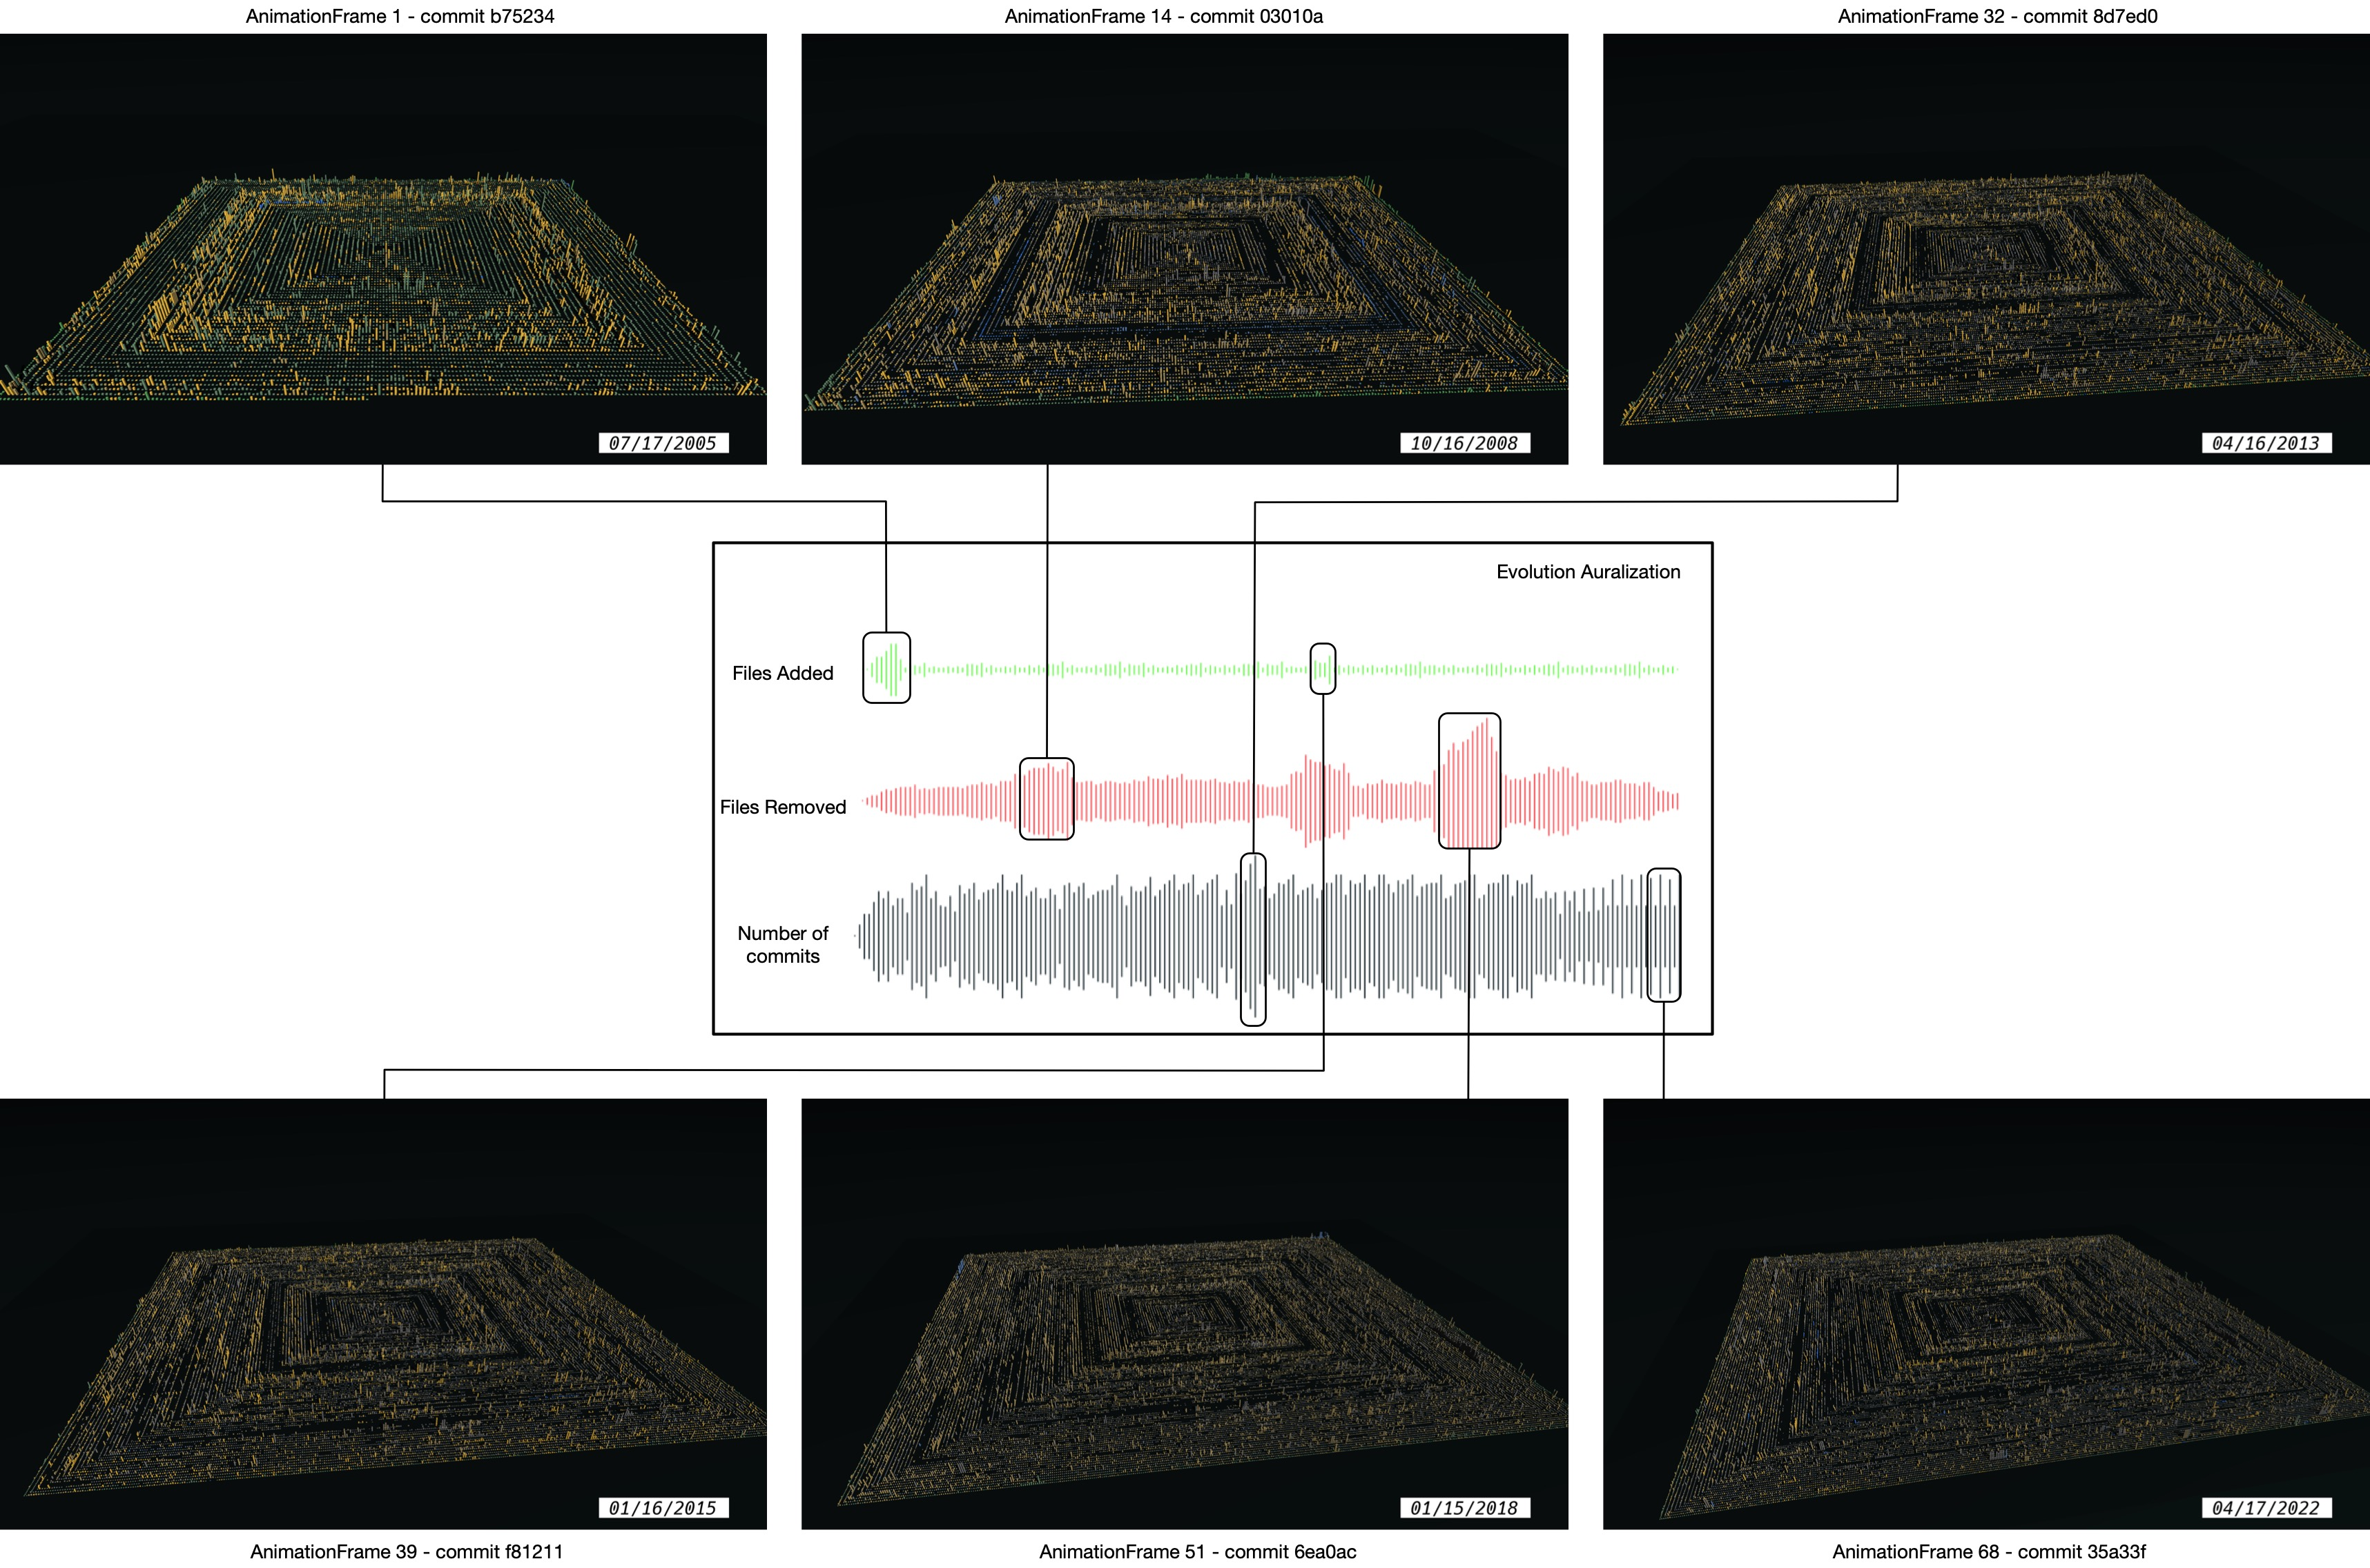
\includegraphics[width=\linewidth]{LinuxAuralization.jpg}
    \caption{Frames of Linux's Evoltution} 
    \label{fig:Linux_V7}
\end{figure}
\end{landscape}
We combined our visualization and auralization approach in a video depicting the evolution of Linux.\footnote{\url{https://www.youtube.com/watch?v=iXGQoO7WAA0}} The video shows how the Linux repository evolved in 17 years between April 2005 and April 2022. 

\autoref{fig:Linux_V7} shows a visual representation of sounds generated from Linux, with some frames of its evolution. The video starts with a peak on the number of files added. As we can see from AnimationFrame 1, the size of the system became massive in the first three months of evolution. Linus Torvalds, the author of Linux and the maintainer of the repository in April 2005, created a new repository to host the Linux codebase instead of converting the existing one to Git. He explained the reasons for this choice in the first commit.\footnote{\url{https://github.com/torvalds/linux/commit/1da177e4}}

In October 2008, as shown in AnimationFrame 14, there was a peak in the number of removed files. Consequently, the prevalence of the sound representing deleted files is high. In this video frame, the center of the spiral starts to become sparse. As highlighted in AnimationFrame 32, the development activity was constant and very high during this 
seventeen-year interval. This frame has many files painted with a bright color, meaning they were updated slightly before the frame's date. 
In the end, from AnimationFrame 68, we can understand the actual size of the system.



\textbf{Conclusion:}
 We saw how the codebase of Linux evolved since their move to git. The development activity was constant throughout these 17 years. The codebase started with 19,705 files and reached 77,183 in April 2022, almost four times its original size. During this time, they evolved the kernel to develop new features and started a process to slowly remove the files that were added 17 years ago. As we can see, the center of the spiral began to become sparse. Nonetheless, it still holds many files, which means that the current version of Linux relies on files written more than 17 years ago. 

\bigbreak



\begin{figure}[ht]
    \begin{subfigure}{0.48\textwidth}
        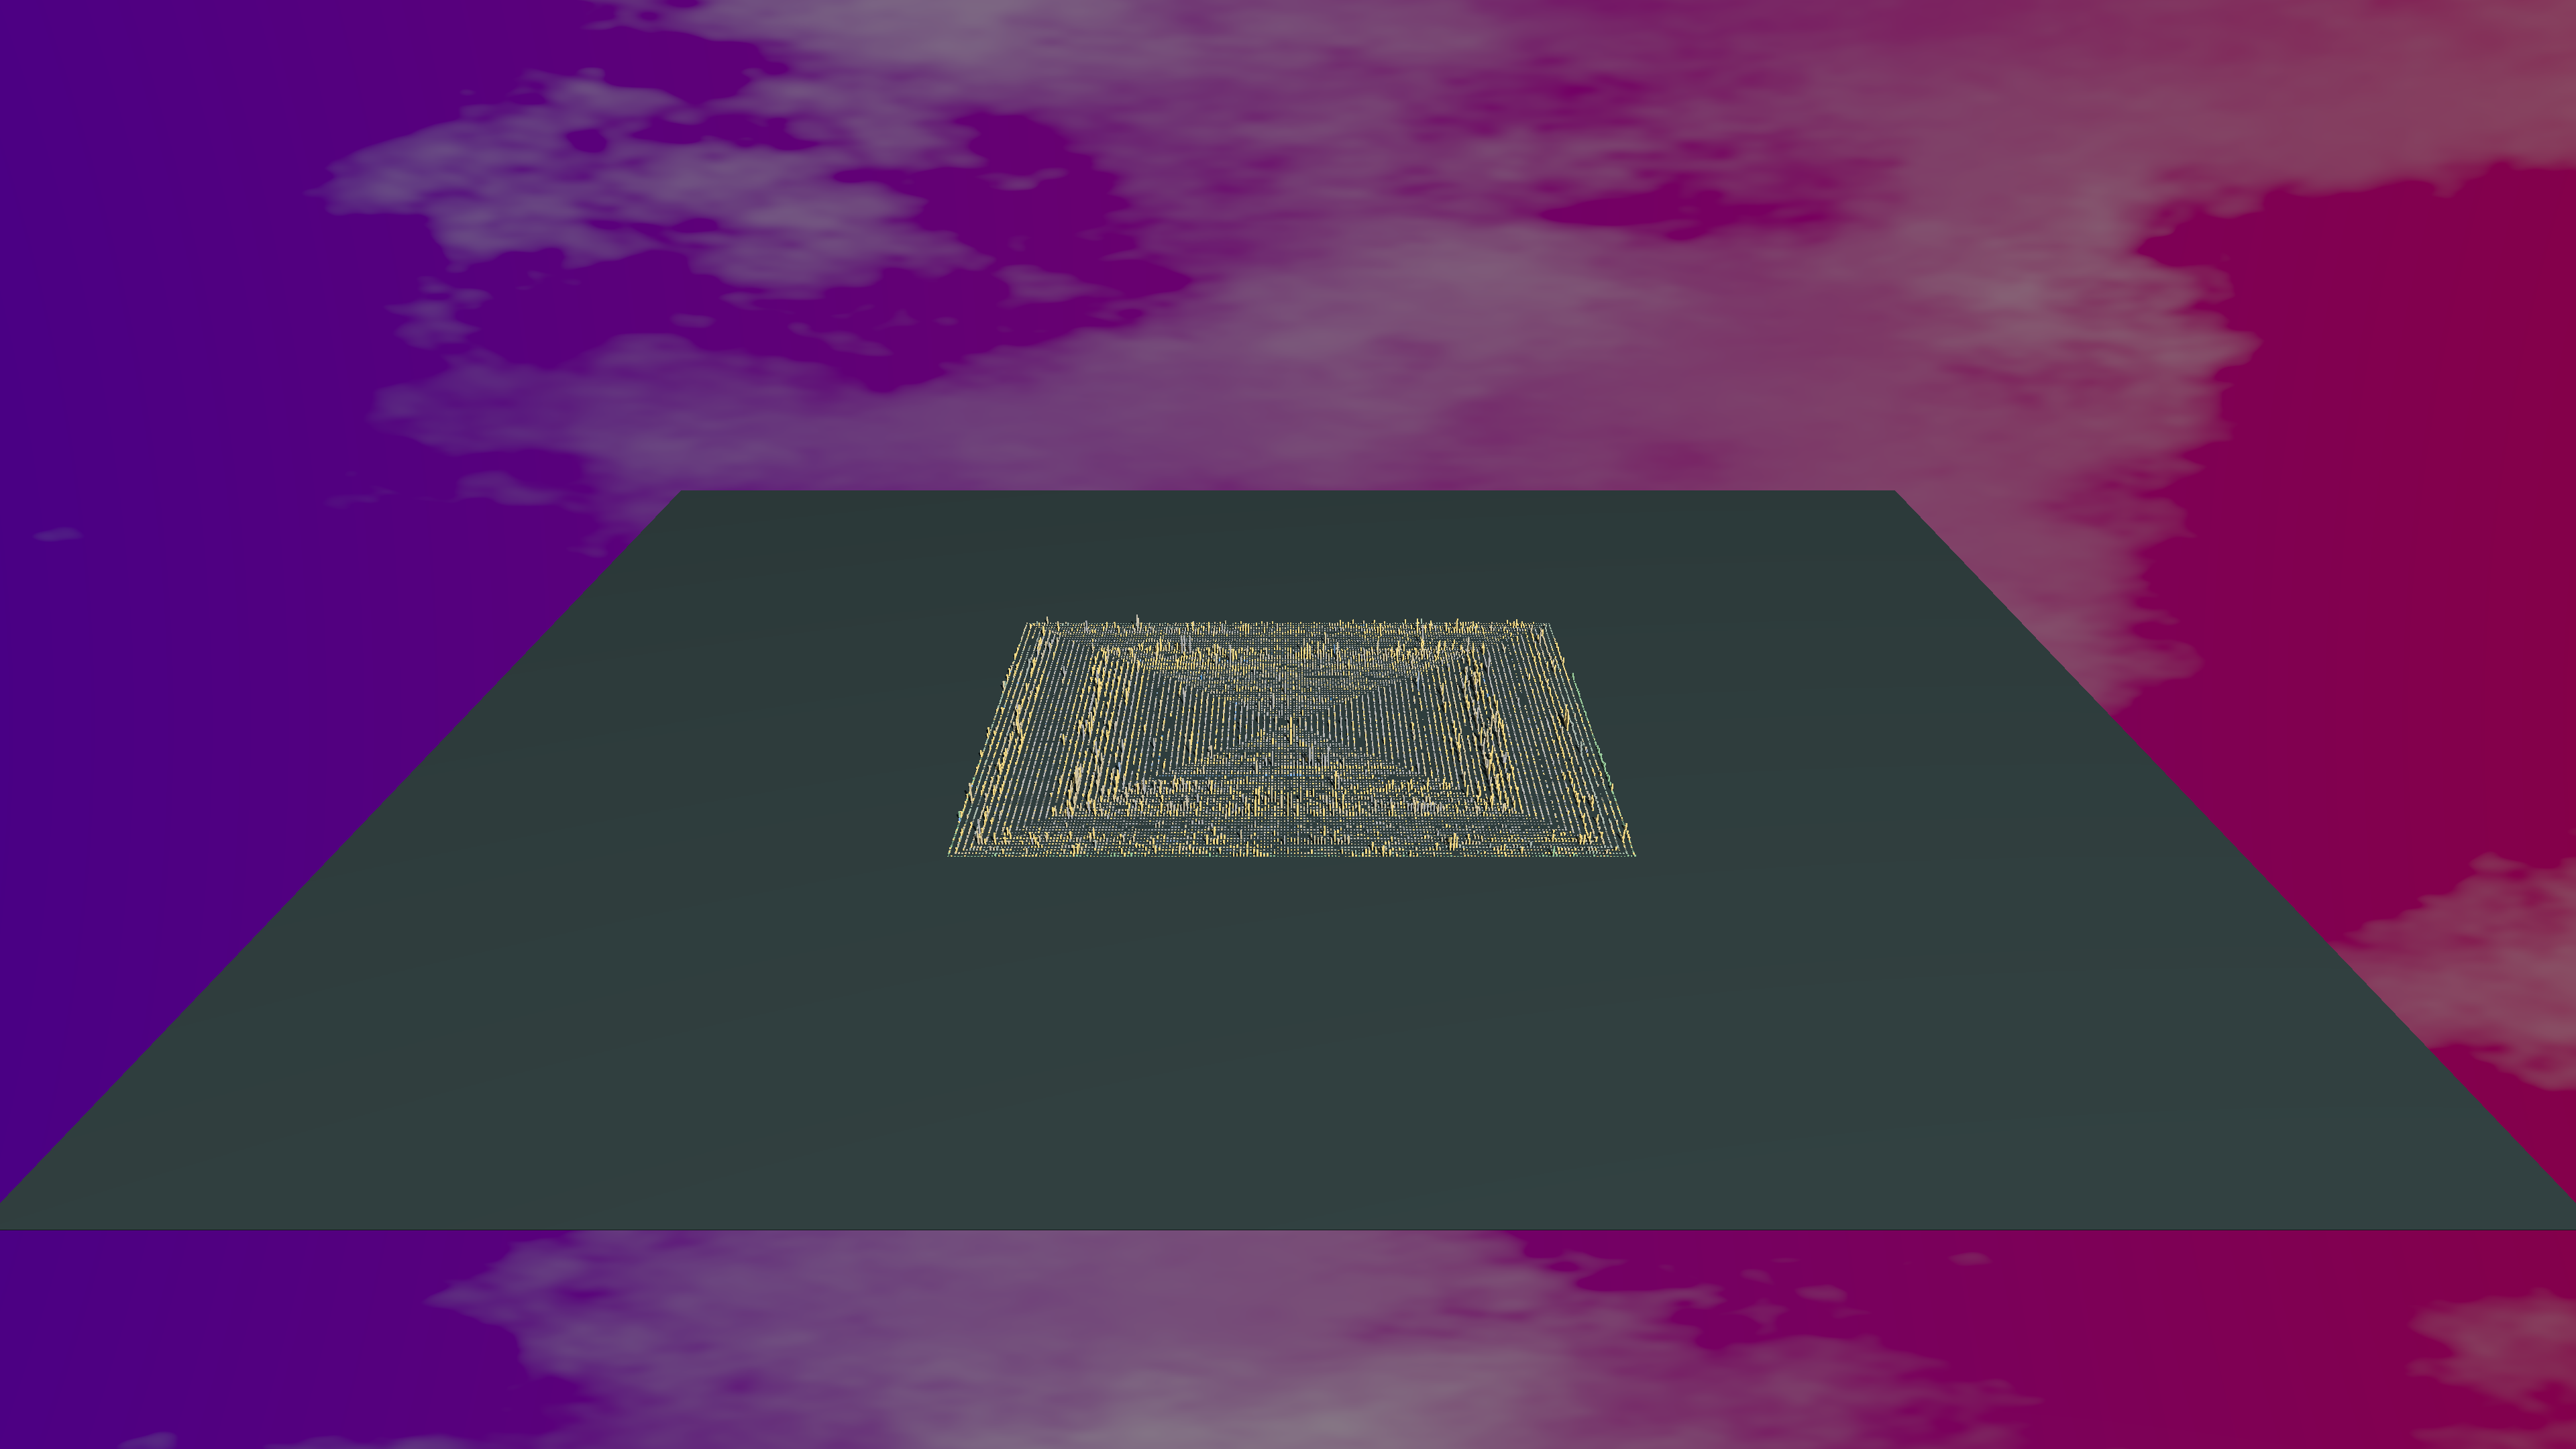
\includegraphics[width=\linewidth]{Linux/Animation001.png}
        \caption{Linux in April 2006 (1 year)} 
        \label{fig:Linux_V7_S1}
    \end{subfigure}\hspace*{\fill}
    \begin{subfigure}{0.48\textwidth}
        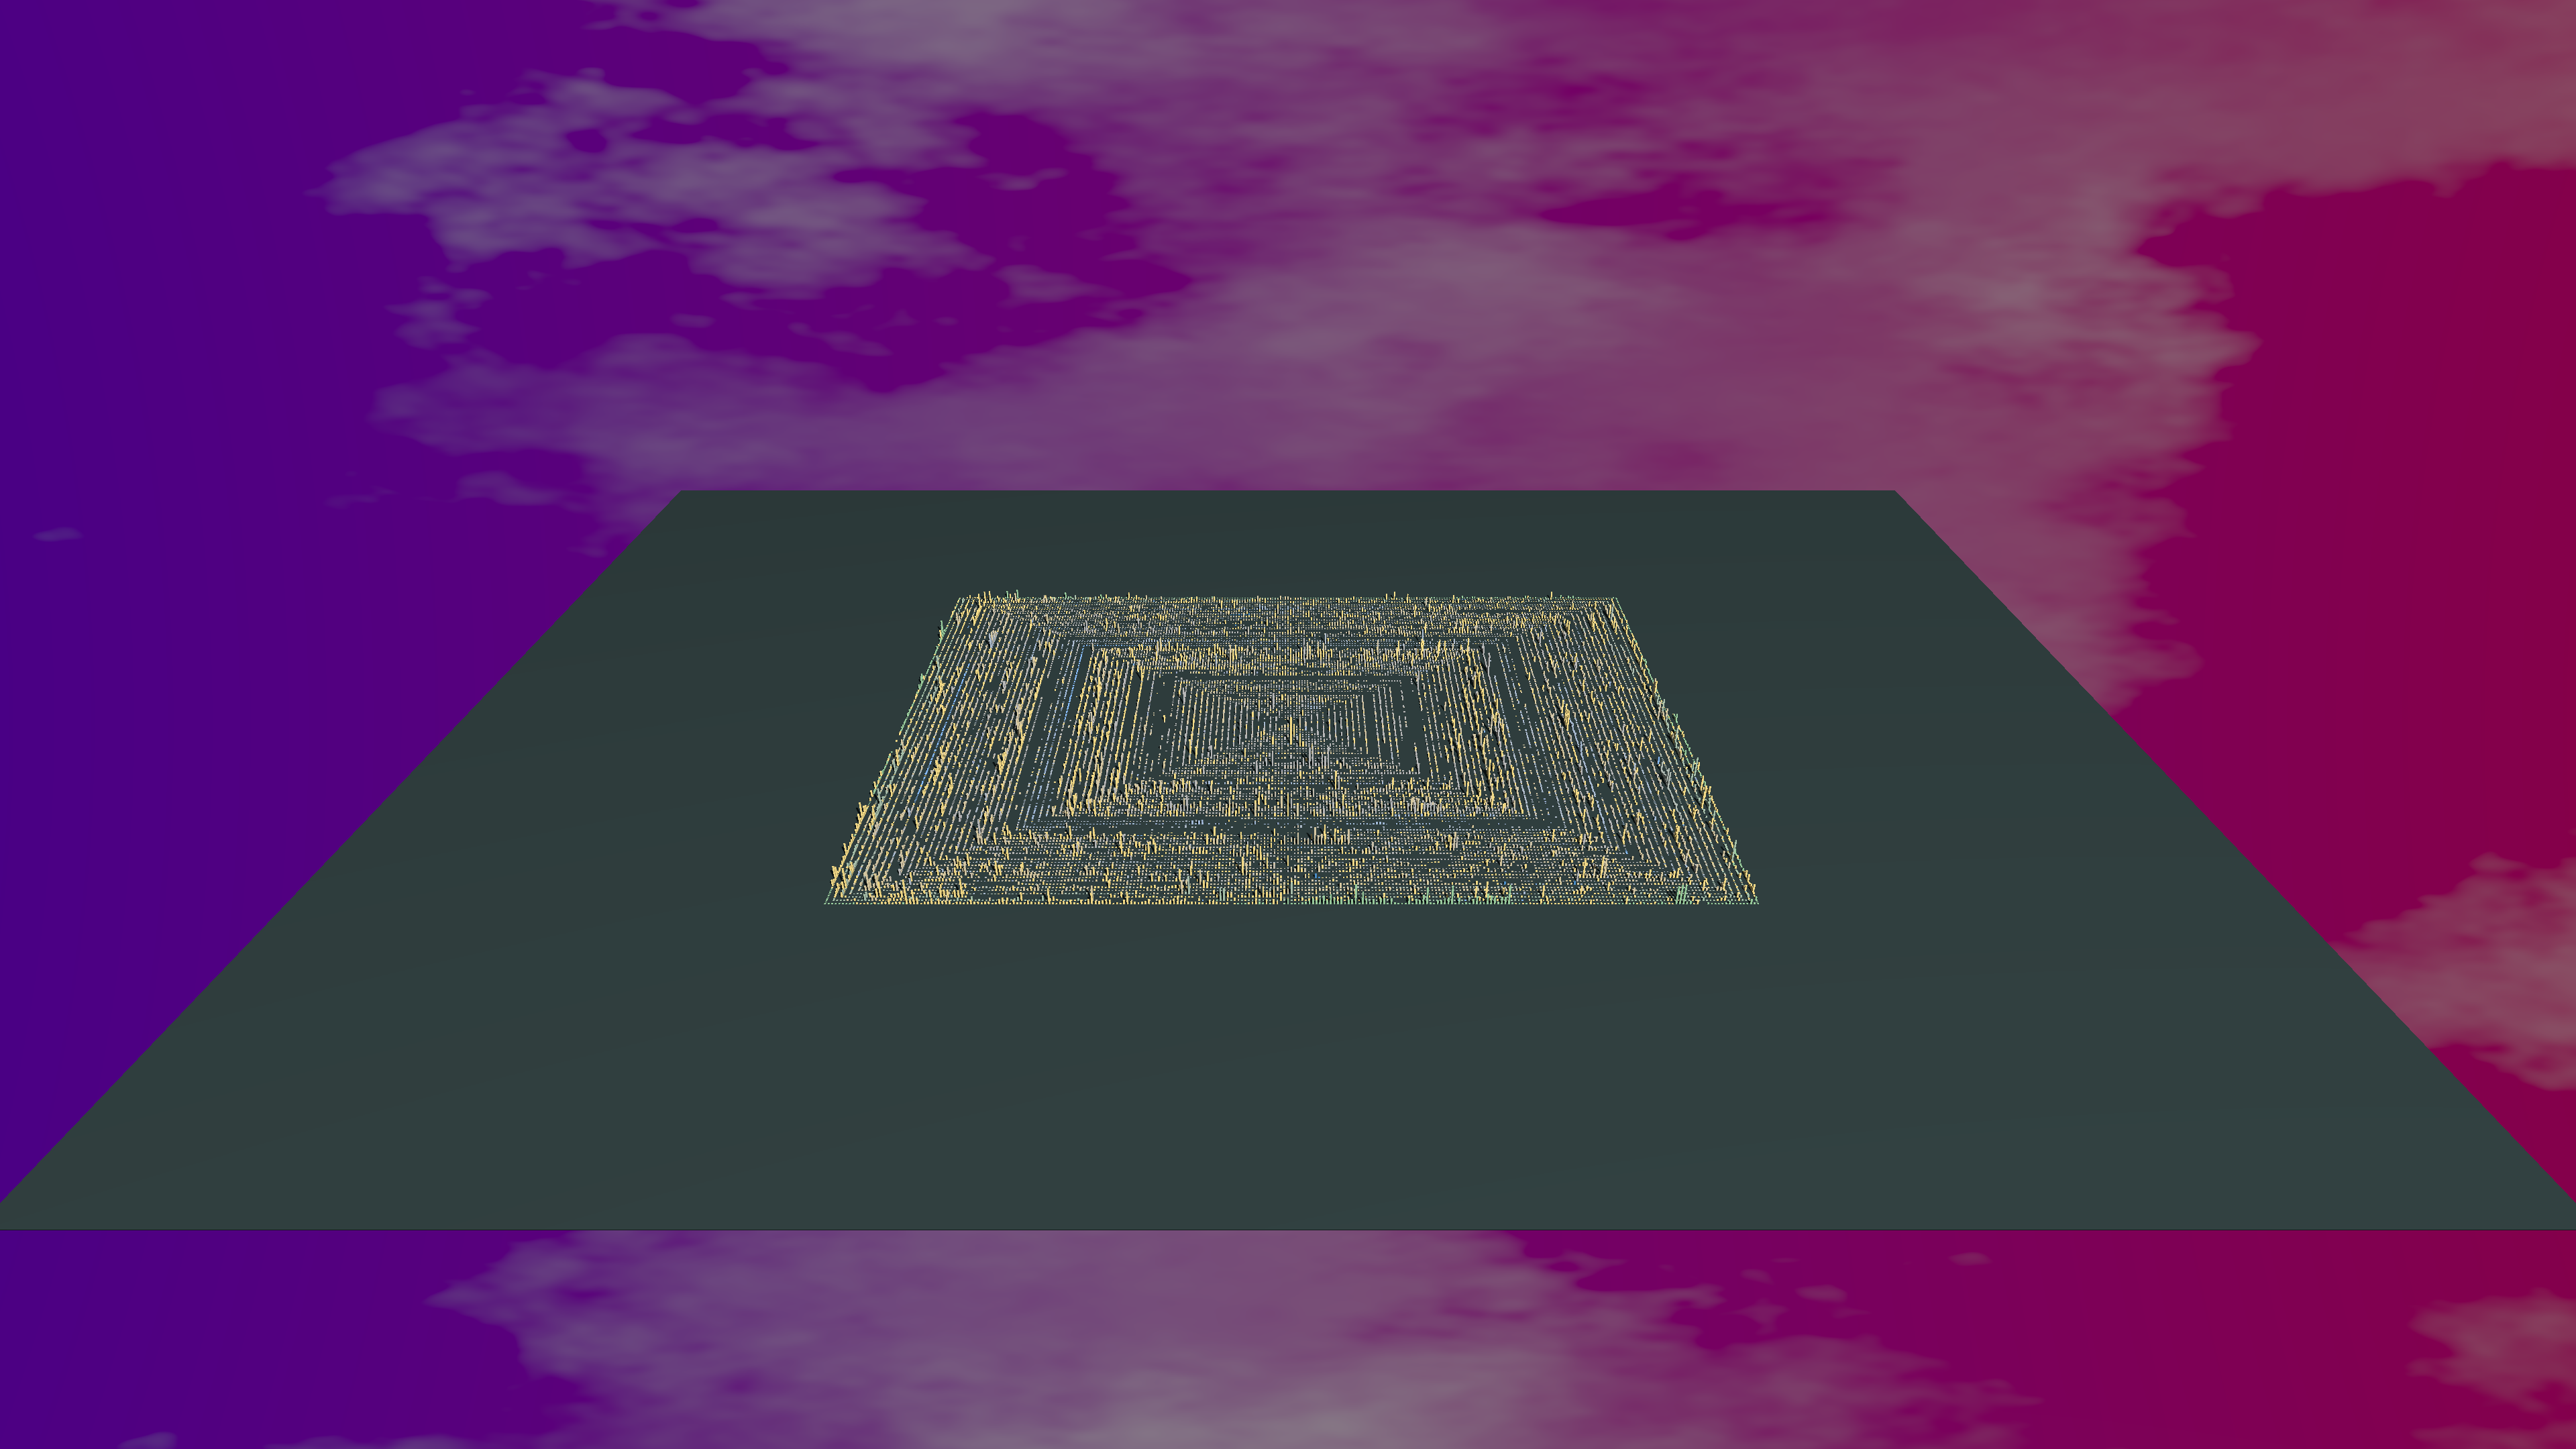
\includegraphics[width=\linewidth]{Linux/Animation004.png}
        \caption{Linux in April 2009 (4 year)} 
        \label{fig:Linux_V7_S2}
    \end{subfigure}
    \medskip
    \begin{subfigure}{0.48\textwidth}
        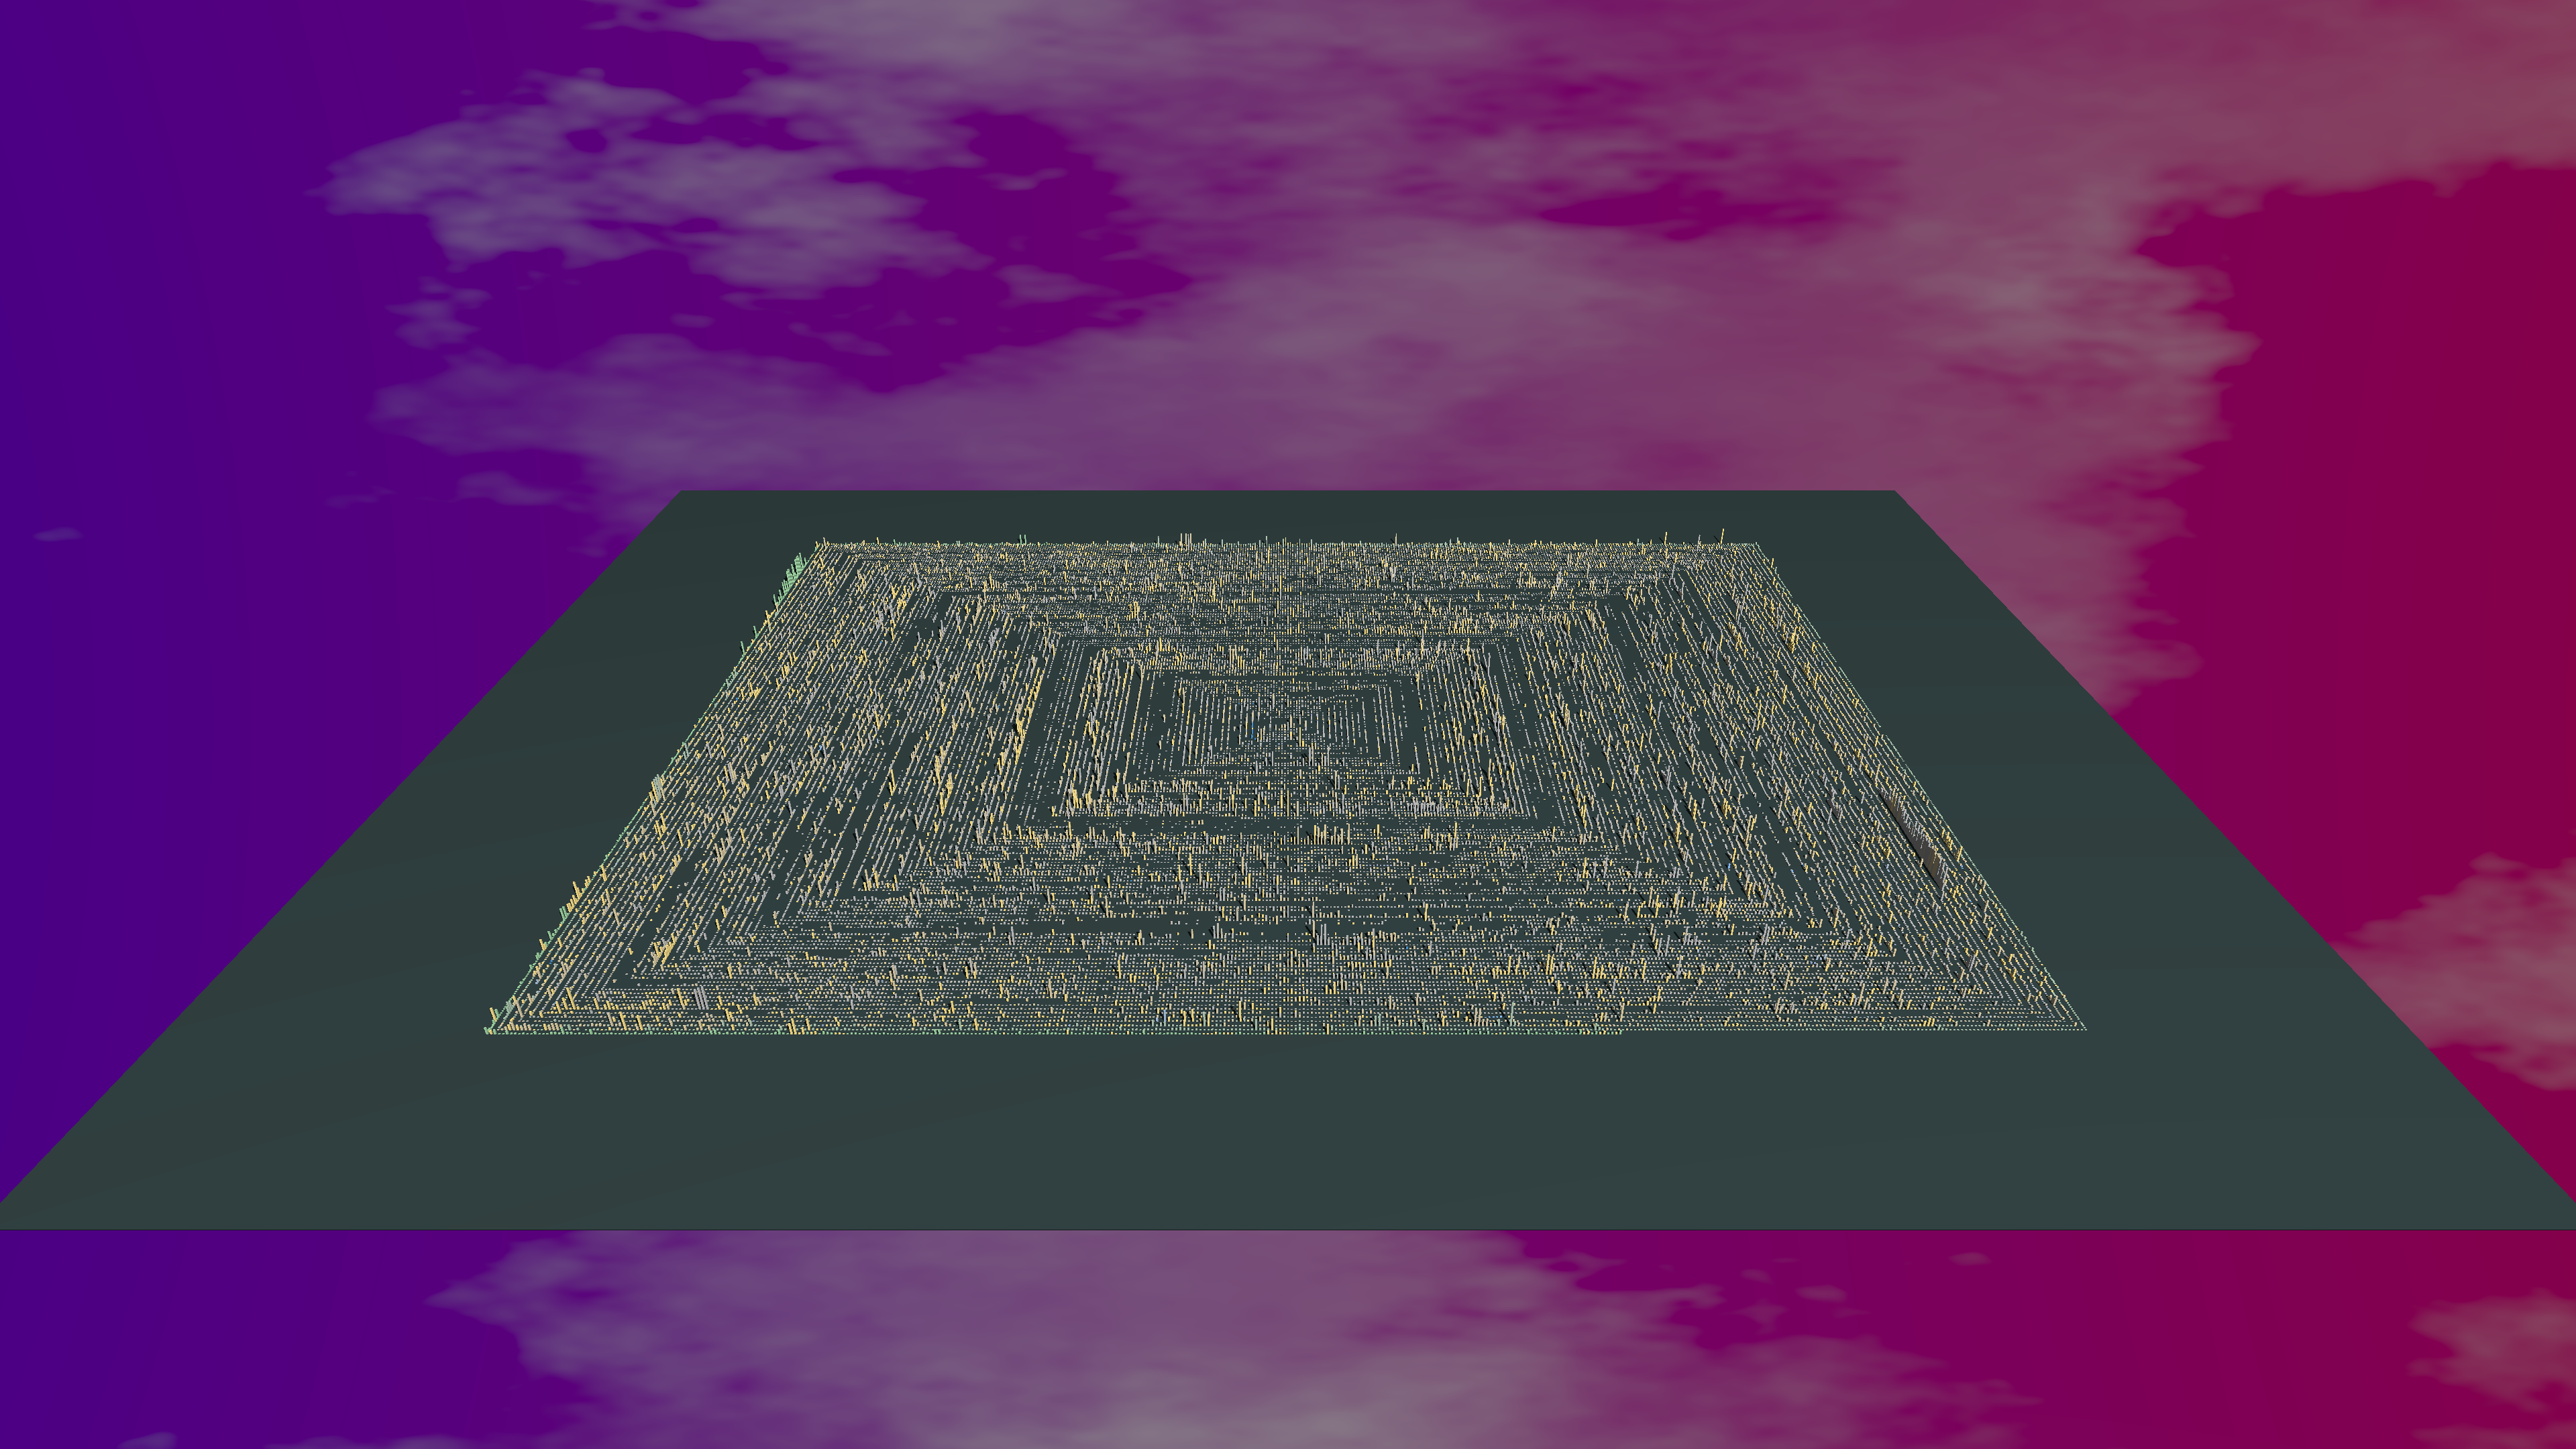
\includegraphics[width=\linewidth]{Linux/Animation012.png}
        \caption{Linux in April 2017 (12 year)} 
        \label{fig:Linux_V7_S3}
    \end{subfigure}\hspace*{\fill}
    \begin{subfigure}{0.48\textwidth}
        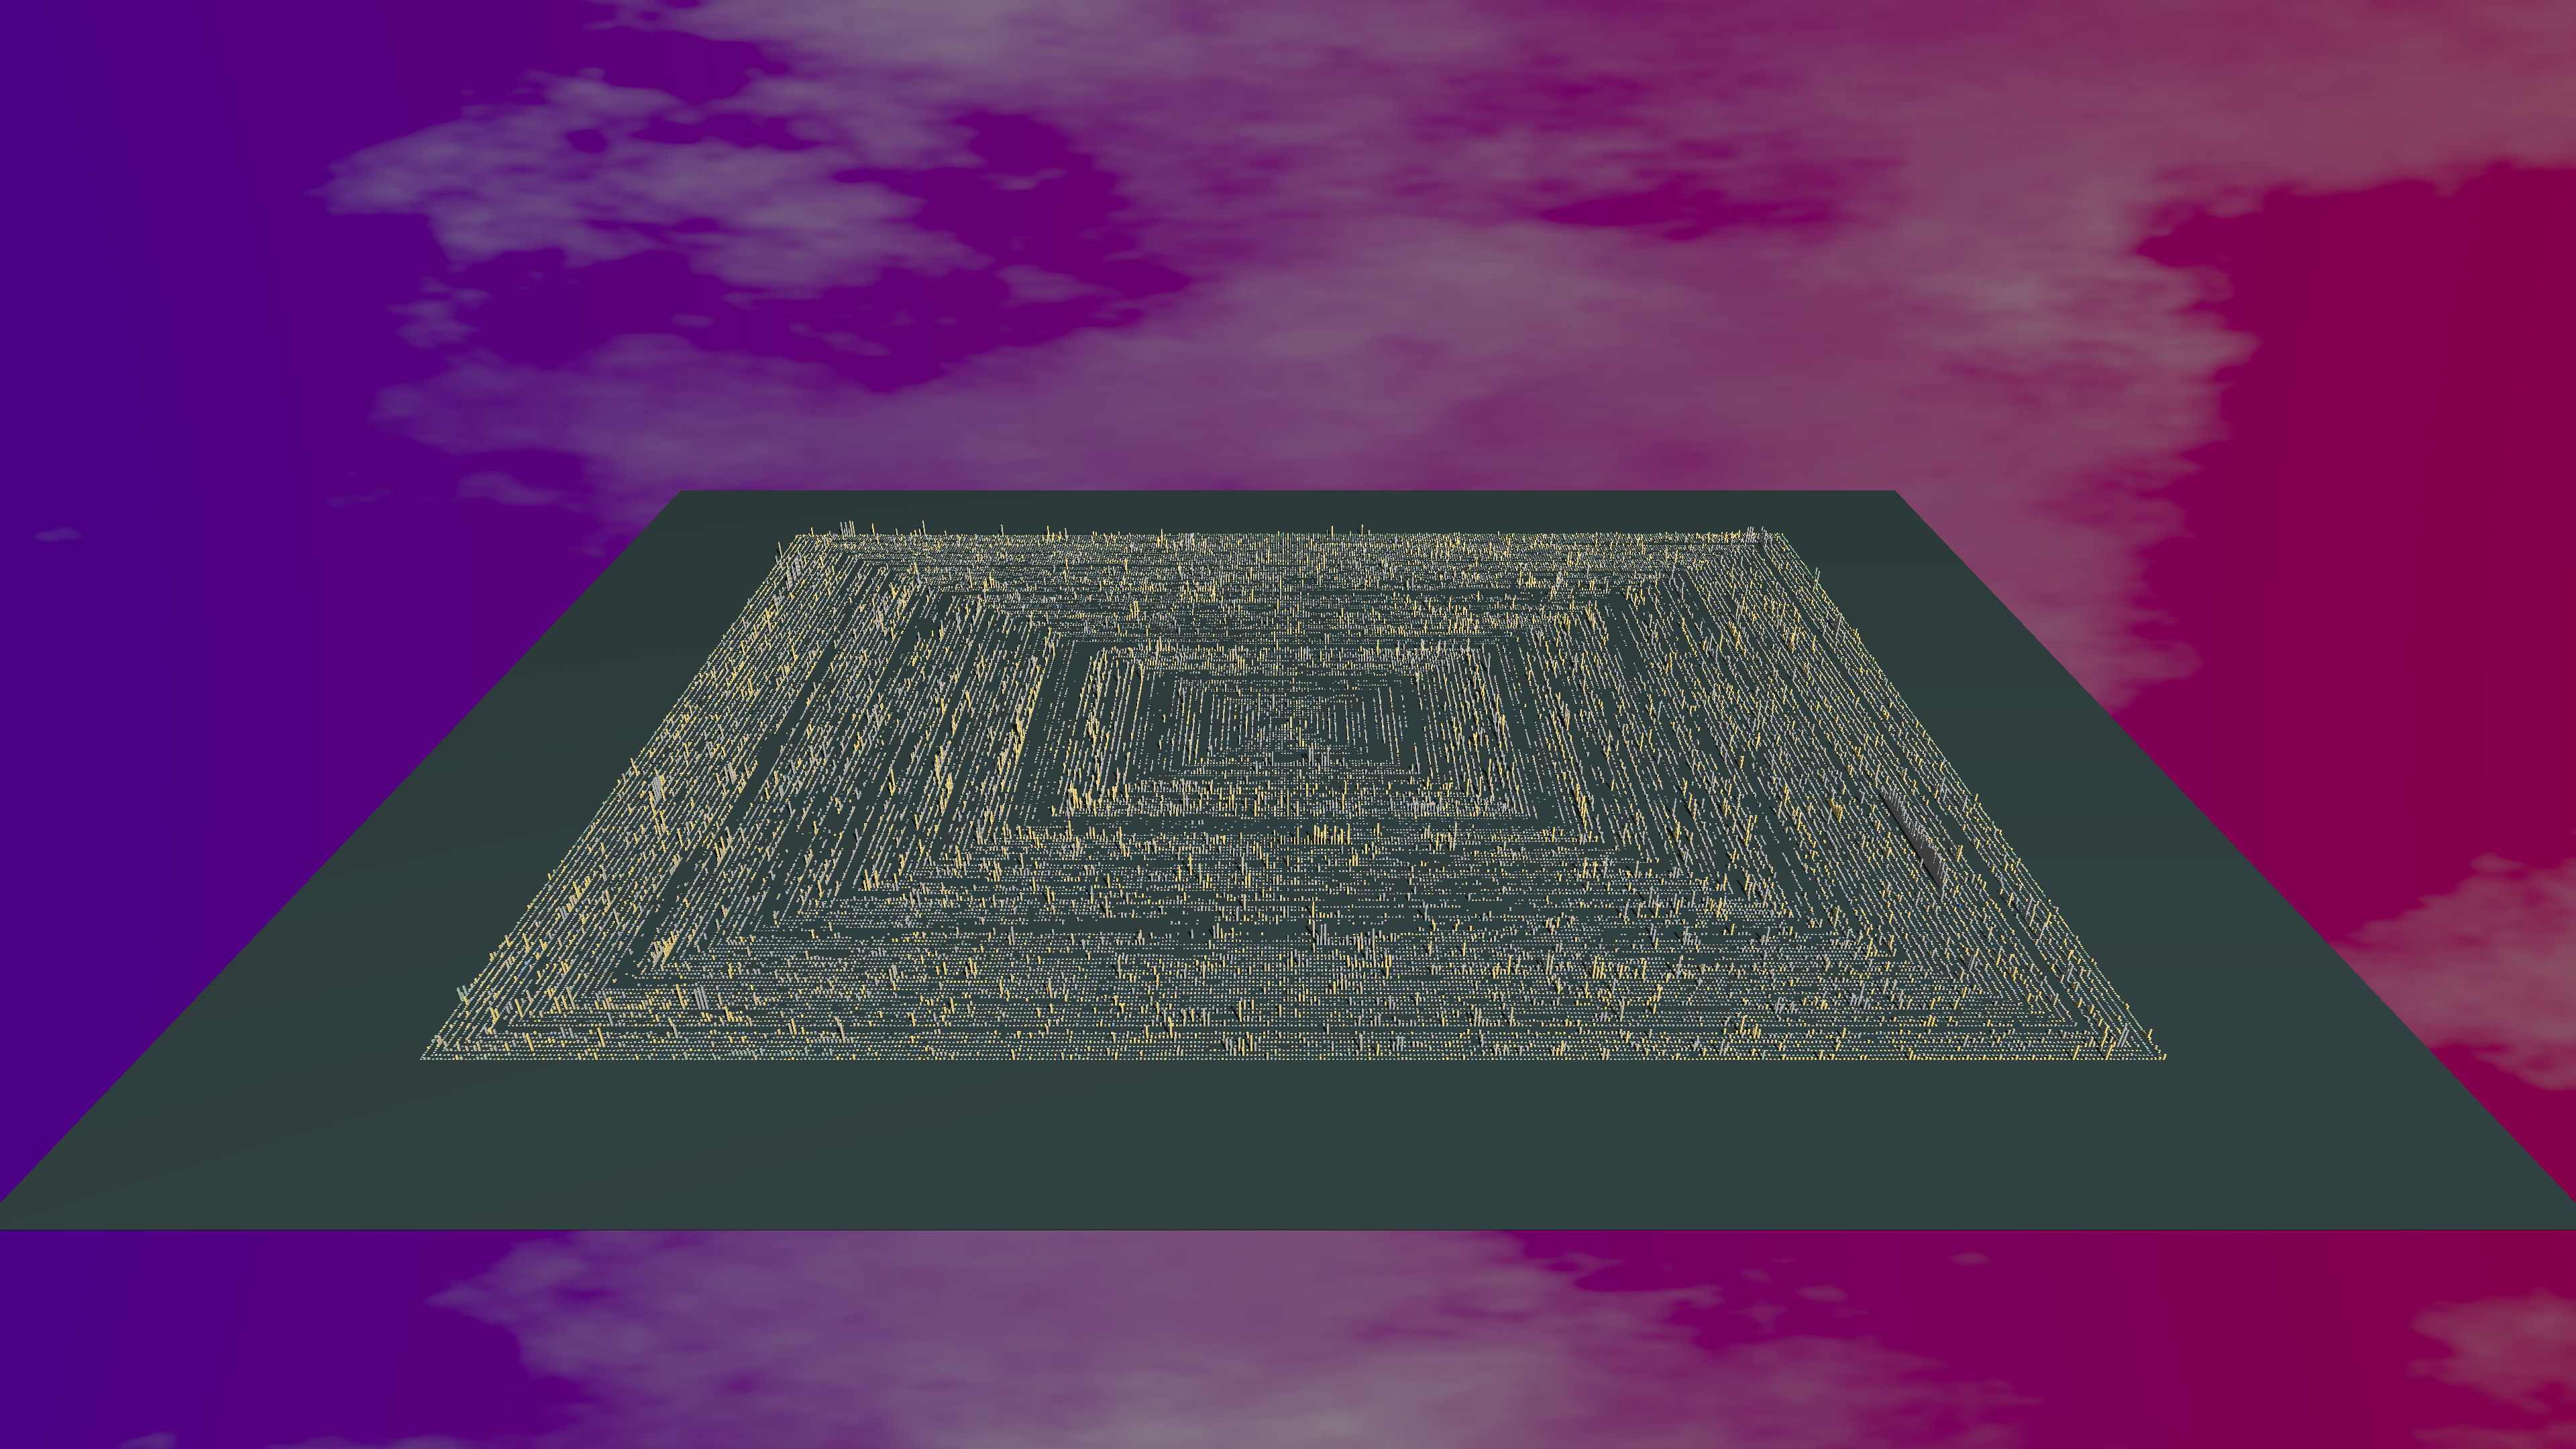
\includegraphics[width=\linewidth]{Linux/Animation014.png}
        \caption{Linux in April 2019  (14 year)} 
        \label{fig:Linux_V7_S4}
    \end{subfigure}
    \medskip
    \begin{subfigure}{0.48\textwidth}
        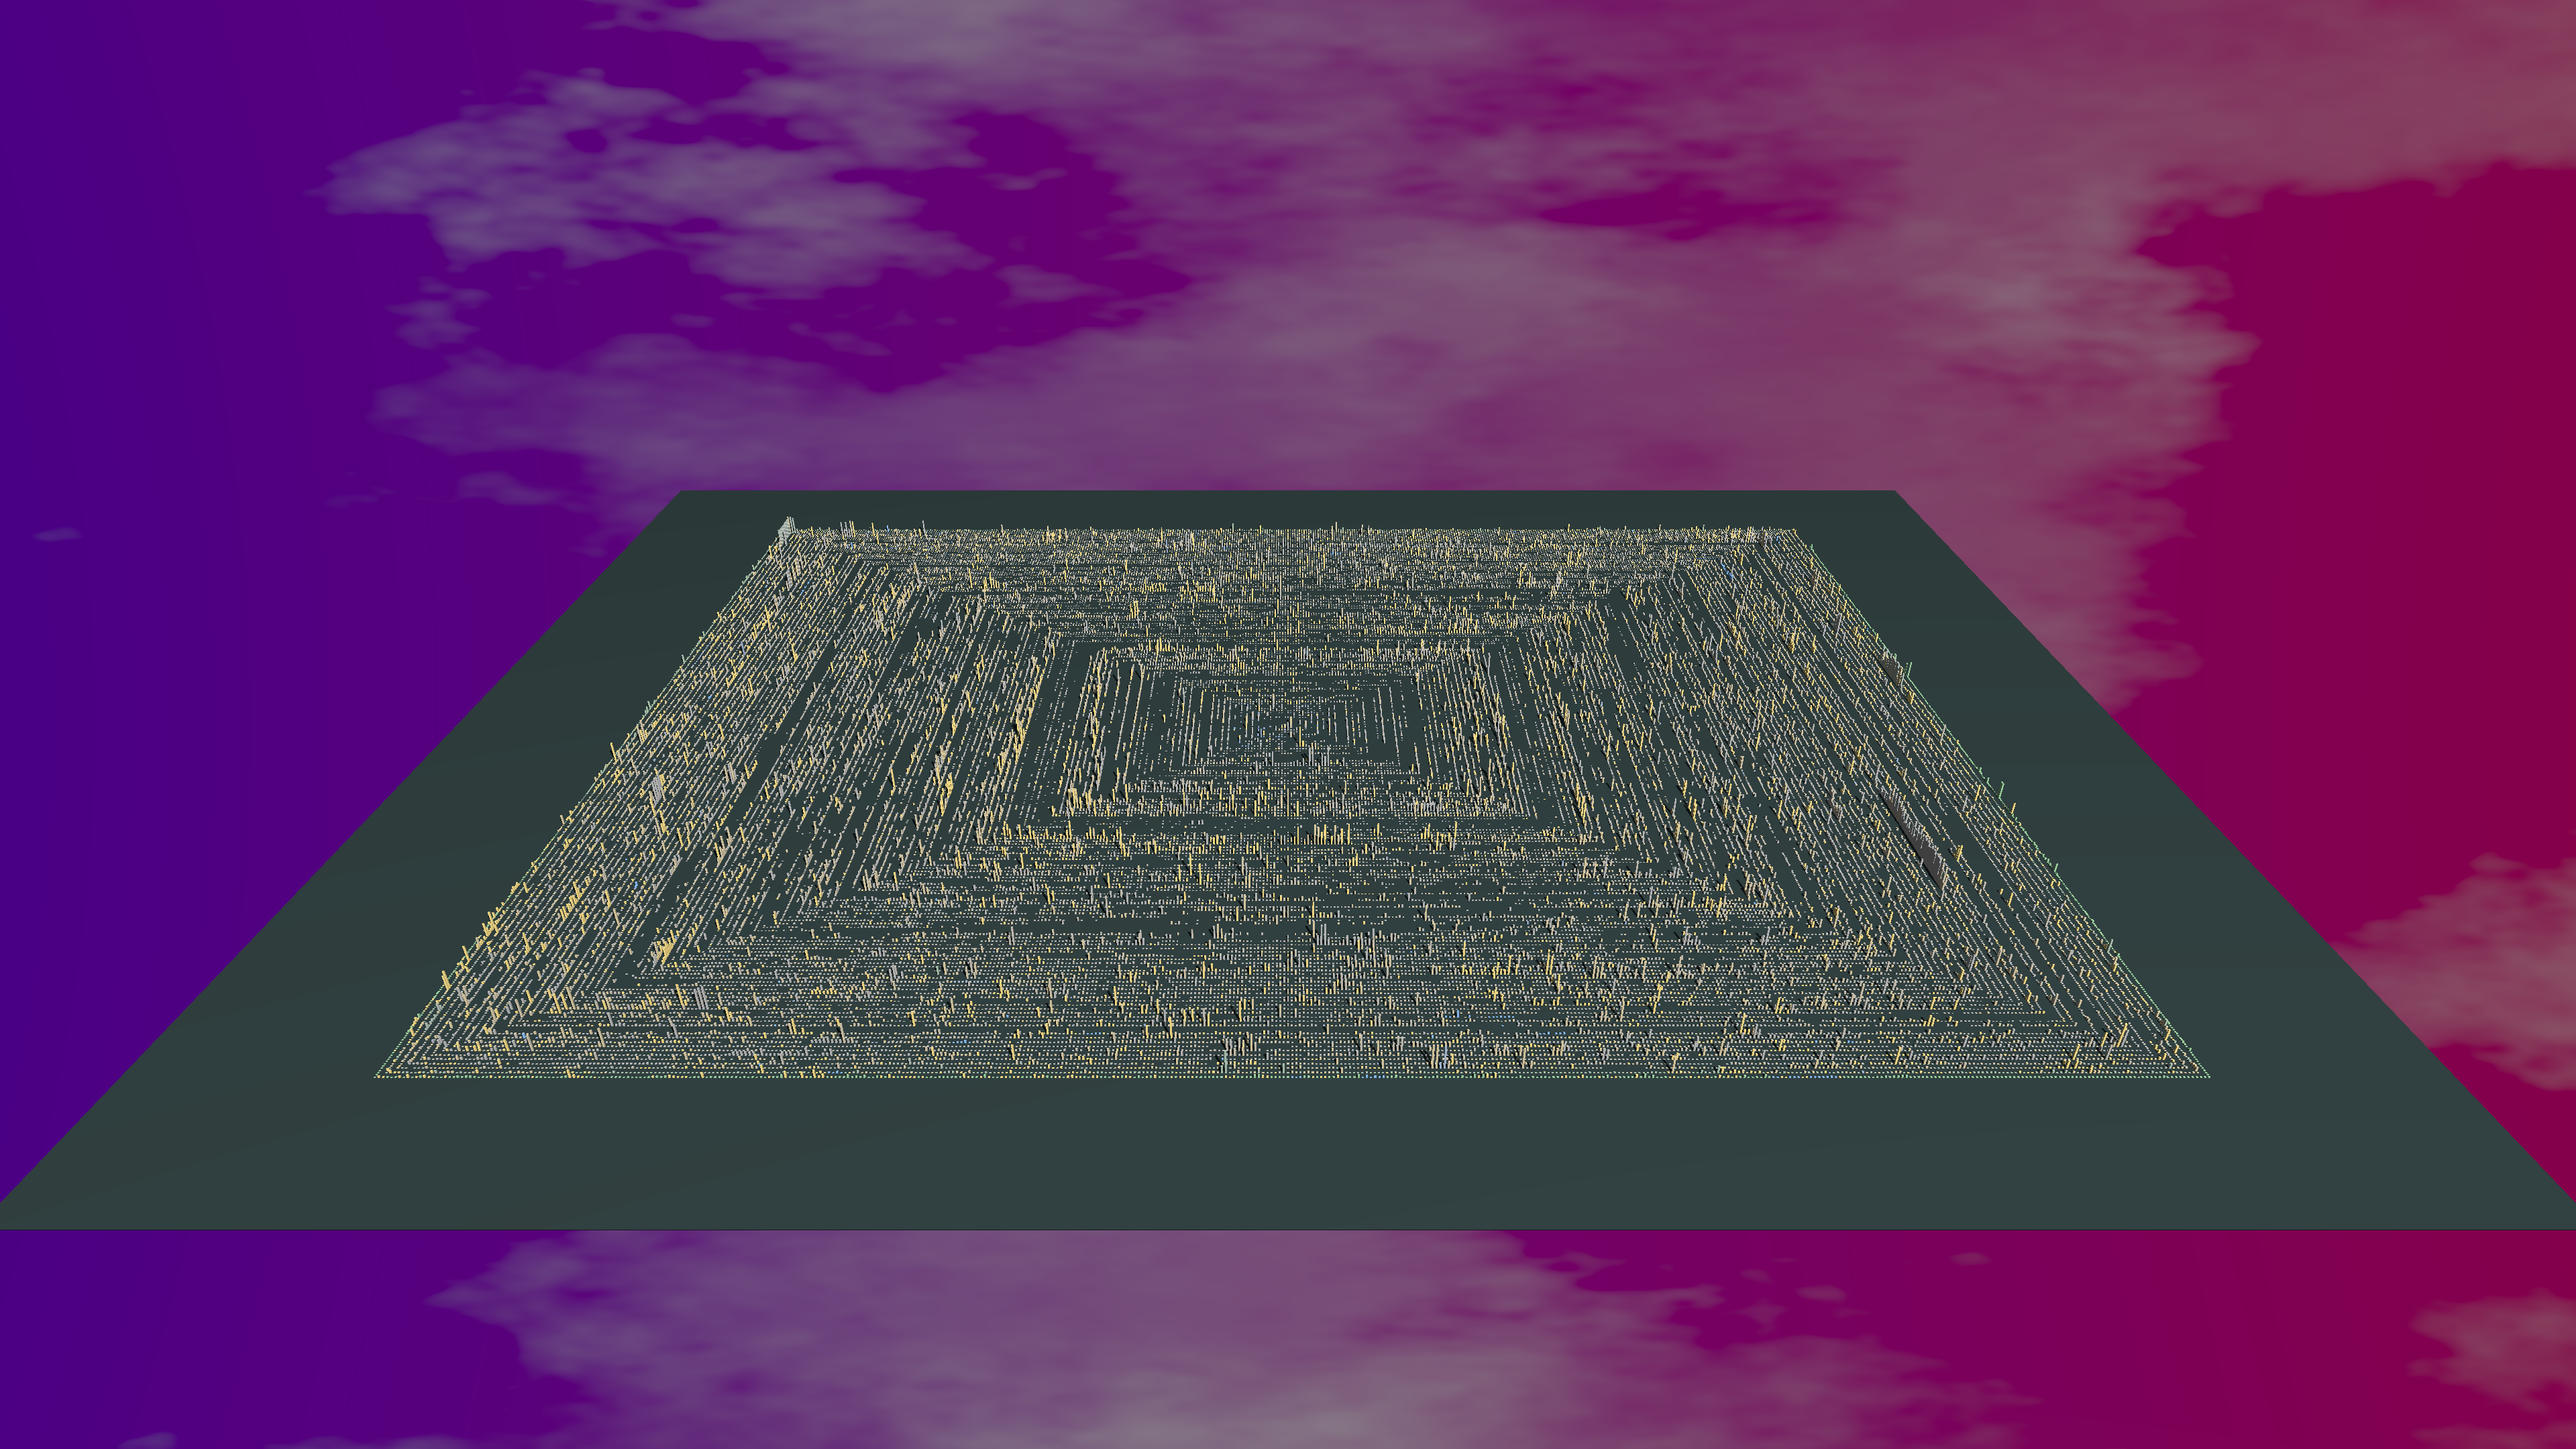
\includegraphics[width=\linewidth]{Linux/Animation015.png}
        \caption{Linux in April 2020 (15 year)} 
        \label{fig:Linux_V7_S5}
    \end{subfigure}\hspace*{\fill}
    \begin{subfigure}{0.48\textwidth}
        \includegraphics[width=\linewidth]{Linux/Animation017.png}
        \caption{Linux in April 2022 (17 year)} 
        \label{fig:Linux_V7_S6}
    \end{subfigure}
    
    \caption{Hot spots during the evolution of Linux} 
    \label{fig:Linux_V7}
\end{figure}

\clearpage
\section{Summary}

To give the reader an idea about the size of the systems, we took the last AnimationFrame of each project and put them next to each other in \autoref{fig:SizeComparison}. Even though Linux was initially bigger than LibreOffice, the latter grew sharply in the last year, overtaking the biggest repository on GitHub. Furthermore, we can observe each system's different development paths. ArgoUML is the only repository that removed all the old files. Elasticsearch seems to rely on its core heavily. As we can see, it is dense, and we also saw during its evolution that it was updated frequently. Of course, these two projects have different histories. ArgoUML has commits dated 1998, and the first commit of Elasticsearch was made in 2013. Equally important is the state of Linux and LibreOffice. Both of them started to move some files from the core to the edges. However, both work with files older than 17 years. 

\begin{figure}[ht]
    \centering
    \includegraphics[width=\linewidth]{SizeComparison.png}
    \caption{Comparison of the projects' state in June 2022.} 
    \label{fig:SizeComparison}
\end{figure}
